\documentclass[12pt,a4paper]{article}
% !TeX root = ../main.tex
\usepackage[utf8]{vntex}
\usepackage[dvipsnames]{xcolor}
\usepackage{colortbl}
%\usepackage[english,vietnam]{babel}
%\usepackage[utf8]{inputenc}
%\usepackage[colorlinks=true, linkcolor=red, urlcolor=red]{hyperref}
%\usepackage[utf8]{inputenc}
%\usepackage[francais]{babel}
\usepackage{a4wide,amssymb,epsfig,latexsym,array,hhline,fancyhdr}
\usepackage[normalem]{ulem}
\usepackage{lipsum}
%\usepackage{soul}
\usepackage{caption}
\usepackage{float}
\renewcommand{\figurename}{}
\usepackage[nointegrals]{wasysym}
\usepackage{enumitem}
\usepackage[makeroom]{cancel}
\usepackage{amsmath}
\usepackage{amsfonts}
\usepackage{amssymb}
\usepackage{amsthm}
\usepackage{multicol,longtable,amscd}
\usepackage{diagbox}%Make diagonal lines in tables
\usepackage{booktabs}
\usepackage{alltt}
\usepackage[framemethod=tikz]{mdframed}% For highlighting paragraph backgrounds
\usepackage{caption,subcaption}
\usepackage{listings}
\usepackage{color}
\usepackage{lastpage}
\usepackage{algorithm}
\usepackage{algpseudocode}
\usepackage{color}
\usepackage{graphicx}							% Standard graphics package
\usepackage{array}
\usepackage{tabularx, caption}
\usepackage{multirow}
\usepackage{multicol}
\usepackage{rotating}
\usepackage{graphics}
\usepackage{geometry}
\usepackage{setspace}
\usepackage{epsfig}
\usepackage{tikz}
\usepackage{placeins} 
\usepackage{matlab-prettifier}  % Nếu cài gói này (rất đẹp cho MATLAB)
% \usepackage{listings}
% \usepackage{xcolor}
\lstdefinestyle{PythonStyle}{
    language=Python,
    basicstyle=\ttfamily\small,
    keywordstyle=\color{blue}\bfseries,
    stringstyle=\color{red},
    commentstyle=\color{green!50!black}\itshape,
    numberstyle=\tiny\color{gray},
    numbers=left,
    numbersep=5pt,
    backgroundcolor=\color{yellow!10},
    frame=single,
    breaklines=true,
    showstringspaces=false,
    tabsize=4,
}
\lstdefinestyle{SQLStyle}{
    language=SQL,
    basicstyle=\ttfamily\footnotesize,
    keywordstyle=\color{blue}\bfseries,
    stringstyle=\color{red},
    commentstyle=\color{green!50!black}\itshape,
    backgroundcolor=\color{yellow!10},
    frame=single,
    breaklines=true,
    showstringspaces=false,
    columns=fullflexible,
    keepspaces=true,
    morekeywords={ROLLUP,CUBE,FILTER,OVER,PARTITION,ROW_NUMBER,COALESCE,TO_CHAR,EXTRACT,EPOCH,INTERVAL},
}

\lstdefinestyle{mat}{language=Matlab,basicstyle=\ttfamily\footnotesize,
  commentstyle=\color{gray},keywordstyle=\color{blue},numbers=left,
  numberstyle=\tiny,breaklines=true,frame=single,columns=fixed,
  keepspaces=true,showstringspaces=false}

\usetikzlibrary{arrows,arrows.meta,backgrounds,positioning,calc,fit,shapes.multipart,shapes.geometric,decorations.pathreplacing}

% ---------- Bộ màu và style dùng chung cho mọi sơ đồ (trùng với biểu đồ trong src/report/make_figures.py)
\definecolor{dwBlue}{HTML}{2A78D6}
\definecolor{dwBlueDark}{HTML}{184F95}
\definecolor{dwOrange}{HTML}{EB6834}
\definecolor{dwAqua}{HTML}{1BAF7A}
\definecolor{dwYellow}{HTML}{EDA100}
\definecolor{dwViolet}{HTML}{6250D6}
\definecolor{dwInk}{HTML}{0B0B0B}
\definecolor{dwInkTwo}{HTML}{52514E}
\definecolor{dwMuted}{HTML}{898781}
\definecolor{dwLine}{HTML}{C3C2B7}
\definecolor{dwPaper}{HTML}{F7F6F2}
\tikzset{
  dwbox/.style={draw=#1!70!black, line width=0.5pt, fill=#1!7, rounded corners=3pt, align=center,
                font=\footnotesize, inner sep=4pt},
  dwbox/.default=dwBlue,
  dwhead/.style={draw=#1!80!black, line width=0.5pt, fill=#1, text=white, font=\footnotesize\bfseries,
                 rounded corners=0pt, inner sep=3pt, align=center},
  dwhead/.default=dwBlue,
  dwfield/.style={draw=dwLine, line width=0.4pt, fill=white, font=\scriptsize\ttfamily, inner sep=2pt,
                  anchor=north, align=left},
  dwarrow/.style={-{Stealth[length=2.2mm,width=1.6mm]}, line width=0.6pt, draw=dwInkTwo},
  dwdash/.style={-{Stealth[length=2mm,width=1.5mm]}, line width=0.5pt, draw=dwMuted, dashed},
  dwlabel/.style={font=\scriptsize, text=dwInkTwo, fill=white, inner sep=1.2pt},
  dwnote/.style={font=\scriptsize, text=dwMuted, align=center},
  dwdb/.style={cylinder, shape border rotate=90, aspect=0.18, draw=#1!70!black, line width=0.5pt, fill=#1!10,
               align=center, font=\footnotesize, inner sep=3pt},
  dwdb/.default=dwBlue,
}
% \dwtable{tên node}{vị trí}{tiêu đề}{màu}{bề rộng}{danh sách cột, cách nhau bởi dấu phẩy}
% Tạo node <tên> (tiêu đề) và <tên>-1, <tên>-2, ... cho từng cột để vẽ liên kết tới đúng cột.
\newcommand{\dwtable}[6]{%
  \node[dwhead=#4, text width=#5, inner sep=2.5pt] (#1) at (#2) {#3};
  \xdef\dwprev{#1}%
  \foreach \dwf [count=\dwi] in {#6} {%
    \node[dwfield, text width=#5, inner sep=2.5pt] (#1-\dwi) at (\dwprev.south) {\dwf};
    \xdef\dwprev{#1-\dwi}%
  }%
}

%\usepackage{pstcol} % PSTricks with the standard color package
\usepackage[normalem]{ulem}

\newtheorem{theorem}{{\bf Định lý}}

\newtheorem{property}{{\bf Tính chất}}
\newtheorem{proposition}{{\bf Mệnh đề}}[section]
\floatname{algorithm}{Thuật toán}
\algrenewcommand\algorithmicrequire{\textbf{Đầu vào:}}
\algrenewcommand\algorithmicensure{\textbf{Đầu ra:}}
\newcommand{\TODO}[1]{\textcolor{red}{\textbf{[#1]}}}
\newcommand{\safeimg}[2]{\IfFileExists{#2}{\includegraphics[#1]{#2}}{\fbox{\TODO{chưa có hình: \detokenize{#2}}}}}
\newcommand{\norm}[1]{\left\lVert #1\right\rVert}
\newcommand{\fro}[1]{\norm{#1}_F}
\newcommand{\inst}{\mathcal{I}}
\newtheorem{corollary}[proposition]{{\bf Hệ quả}}
\newtheorem{lemma}[proposition]{{\bf Bổ đề}}
\theoremstyle{definition}
\newtheorem{exer}{Bài toán}
\def\thesislayout{	% A4: 210 × 297
	\geometry{
		a4paper,
		top=25mm,
		bottom=25mm,
		left=35mm,
		right=20mm,
	}
}
\thesislayout

\makeatletter
\renewcommand\paragraph{\@startsection{paragraph}{4}{\z@}%
  {3.25ex \@plus1ex \@minus.2ex}%
  {1ex \@plus.2ex}%
  {\normalfont\normalsize\bfseries}}
\makeatother

\renewcommand{\baselinestretch}{1.5} % Giãn dòng 1.5
% \setlength{\parskip}{6pt} % Spacing after
\usepackage{indentfirst}
\setlength{\parindent}{1cm}

%\usepackage{fancyhdr}
\setlength{\headheight}{40pt}
\pagestyle{fancy}
\fancyhead{} % clear all header fields
\fancyhead[L]{
 \begin{tabular}{rl}
    \begin{picture}(25,15)(0,0)
    \put(0,-8){
\includegraphics[width=8mm, height=8mm]{./Pictures/hcmut.png}}
    %\put(0,-8){\epsfig{width=10mm,figure=hcmut.eps}}
   \end{picture}&
	%\includegraphics[width=8mm, height=8mm]{hcmut.png} & %
	\begin{tabular}{l}
		\textbf{\bf \ttfamily Trường Đại học Bách khoa -- ĐHQG-HCM}\\
		\textbf{\bf \ttfamily Khoa Khoa học và Kỹ thuật Máy tính}
	\end{tabular} 	
 \end{tabular}
}
\fancyhead[R]{
	\begin{tabular}{l}
		\tiny \bf \\
		\tiny \bf 
	\end{tabular}  }
\fancyfoot{} % clear all footer fields
\fancyfoot[L]{\scriptsize \ttfamily Báo cáo bài tập lớn Kho dữ liệu và hệ hỗ trợ quyết định -- CO4031 \\ Năm học 2026 -- 2027}
\fancyfoot[R]{\scriptsize \ttfamily Trang {\thepage}/\pageref{LastPage}}
\renewcommand{\headrulewidth}{0.3pt}
\renewcommand{\footrulewidth}{0.3pt}
%%%
\setcounter{secnumdepth}{4}
\setcounter{tocdepth}{3}
\makeatletter
\newcounter {subsubsubsection}[subsubsection]
\renewcommand\thesubsubsubsection{\thesubsubsection .\@arabic\c@subsubsubsection}
\newcommand\subsubsubsection{\@startsection{subsubsubsection}{4}{\z@}%
                                     {-3.25ex\@plus -1ex \@minus -.2ex}%
                                     {1.5ex \@plus .2ex}%
                                     {\normalfont\normalsize\bfseries}}
\newcommand*\l@subsubsubsection{\@dottedtocline{3}{7.0em}{3.5em}}
\newcommand*{\subsubsubsectionmark}[1]{}
\makeatother

\everymath{\color{black}}%make in-line maths symbols blue to read/check easily

\sloppy
\captionsetup[figure]{labelfont={small,bf},textfont={small,it},aboveskip=3pt,belowskip=6pt}
%space remove between caption, figure, and text
%\captionsetup[table]{labelfont={small,bf},textfont={small,it},aboveskip=3pt,belowskip=6pt}
\captionsetup[table]{labelfont={small,bf},textfont={small,it},belowskip=-1pt,aboveskip=7pt}
%space remove between caption, table, and text

%\floatplacement{figure}{H}%forced here float placement automatically for figures
%\floatplacement{table}{H}%forced here float placement automatically for table
%the following settings (11 lines) are to remove white space before or after the figures and tables
%\setcounter{topnumber}{2}
%\setcounter{bottomnumber}{2}
%\setcounter{totalnumber}{4}
%\renewcommand{\topfraction}{0.85}
%\renewcommand{\bottomfraction}{0.85}
%\renewcommand{\textfraction}{0.15}
%\renewcommand{\floatpagefraction}{0.8}
%\renewcommand{\textfraction}{0.1}
\setlength{\floatsep}{5pt plus 2pt minus 2pt}
\setlength{\textfloatsep}{5pt plus 2pt minus 2pt}
\setlength{\intextsep}{10pt plus 2pt minus 2pt}

\thesislayout
%\lstset{
%    language=C,
%    aboveskip=6mm,
%    belowskip=-6mm,
%    backgroundcolor=\color{white},   
%    commentstyle=\color{codegreen},
%    keywordstyle=\color{blue},
%    numberstyle=\tiny\color{codegray},
%    stringstyle=\color{codepurple},
%    basicstyle=\ttfamily,
%    breakatwhitespace=false,         
%    breaklines=true,                 
%    captionpos=b,                    
%    keepspaces=true,                 
%    numbers=left,                    
%    numbersep=5pt,                  
%    showspaces=false,                
%    showstringspaces=false,
%    showtabs=false,                  
%    tabsize=2,
%    frame=tb,
%    framesep=8pt,
%    rulecolor=\color{black},
%    title=\lstname,
%}

\usepackage{listings}
\usepackage{makecell}
\usepackage{xcolor}

%New colors defined below
\definecolor{codegreen}{rgb}{0,0.6,0}
\definecolor{codegray}{rgb}{0.5,0.5,0.5}
\definecolor{codepurple}{rgb}{0.58,0,0.82}
\definecolor{backcolour}{rgb}{0.95,0.95,0.92}

%Code makecel style named "mystyle"
%\lstdefinestyle{mystyle}{
%  backgroundcolor=\color{backcolour}, commentstyle=\color{codegreen},
%  keywordstyle=\color{magenta},
%  numberstyle=\tiny\color{codegray},
%  stringstyle=\color{codepurple},
%  basicstyle=\ttfamily\footnotesize,
%  breakatwhitespace=false,         
%  breaklines=true,                 
%  captionpos=b,                    
%  keepspaces=true,                 
%  numbers=left,                    
%  numbersep=5pt,                  
%  showspaces=false,                
%  showstringspaces=false,
%  showtabs=false,                  
%  tabsize=2
%}

\DeclareMathOperator{\arccot}{arccot}
\renewcommand{\figurename}{\selectfont \bfseries Hình}
\renewcommand{\tablename}{\selectfont \bfseries Bảng}
\newenvironment{Description}{\list{}{%
    \let\makelabel\descriptionlabel    % this comes from the original description environment
    \setlength{\rightmargin}{\leftmargin}% this comes from the original quote environment
    \setlength{\labelwidth}{0pt}%          this is new
    }}{\endlist}
% \addbibresource{citations.bib}

\usepackage[unicode]{hyperref}
\usepackage{xurl}
\AtBeginDocument{
    \renewcommand{\listfigurename}{Danh mục hình}
    \renewcommand{\listtablename}{Danh mục bảng}
}
\newcolumntype{P}[1]{>{\raggedright\arraybackslash}p{#1}}
\hypersetup{urlcolor=blue,linkcolor=black,citecolor=black,colorlinks=true} 
% \usetikzlibrary{arrows,backgrounds}
\definecolor{mathblue}{RGB}{0,114,188}
\definecolor{mGreen}{rgb}{0,0.6,0}
\definecolor{mGray}{rgb}{0.5,0.5,0.5}
\definecolor{mPurple}{rgb}{0.58,0,0.82}
\definecolor{backgroundColour}{rgb}{250,245,239}
\definecolor{lightbg}{rgb}{0.98,0.96,0.94}
\definecolor{cadmiumgreen}{rgb}{0.0, 0.42, 0.24}
\definecolor{ceruleanblue}{rgb}{0.16, 0.32, 0.75}

\lstdefinestyle{CStyle}{
  backgroundcolor=\color{magenta!10},
  commentstyle=\color{mGreen},
  keywordstyle=\color{blue},
  numberstyle=\tiny\color{mGray},
  stringstyle=\color{mPurple},
  basicstyle=\ttfamily\footnotesize,
  breakatwhitespace=true,         
  breaklines=true,                 
  captionpos=b,                    
  keepspaces=true,                 
  numbers=left,                    
  numbersep=5pt,                  
  showspaces=false,                
  showstringspaces=false,
  showtabs=false,                  
  tabsize=2,
  framerule=1pt,
  framesep=5pt,
  aboveskip=12pt,   % Custom top margin
  belowskip=12pt,    % Custom bottom margin
  xleftmargin=12pt,     % <-- Left margin here
  framexleftmargin=12pt, 
  frame=single,
}

%"mystyle" code listing set
%\lstset{style=mystyle}
\lstset{
        literate=%
% Vần a
	{á}{{\'a}}1
	{à}{{\`a}}1
	{ạ}{{\d a}}1
	{ả}{{\h a}}1
	{ã}{{\~ a}}1
	%
	{Á}{{\'A}}1
	{À}{{\`A}}1
	{Ạ}{{\d A}}1
	{Ả}{{\h A}}1
	{Ã}{{\~ A}}1
%
% Vần ă
	{ă}{{\u a}}1
	{ắ}{{\'\abreve }}1
	{ằ}{{\`\abreve }}1
	{ặ}{{\d \abreve }}1
	{ẳ}{{\h \abreve }}1
	{ẵ}{{\~\abreve }}1
	%
	{Ă}{{\u A}}1
	{Ắ}{{\'\ABREVE }}1
	{Ằ}{{\`\ABREVE }}1
	{Ặ}{{\d \ABREVE }}1
	{Ẳ}{{\h \ABREVE }}1
	{Ẵ}{{\~\ABREVE }}1
%
% Vần â
	{â}{{\^ a}}1
	{ấ}{{\'\acircumflex }}1
	{ầ}{{\`\acircumflex }}1
	{ậ}{{\d \acircumflex }}1
	{ẩ}{{\h \acircumflex }}1
	{ẫ}{{\~\acircumflex }}1
	 %
	{Â}{{\^ A}}1
	{Ấ}{{\'\ACIRCUMFLEX }}1
	{Ầ}{{\`\ACIRCUMFLEX }}1
	{Ậ}{{\d \ACIRCUMFLEX }}1
	{Ẩ}{{\h \ACIRCUMFLEX }}1
	{Ẫ}{{\~\ACIRCUMFLEX }}1
%
% Vần đ
	{đ}{{\dj }}1
	{Đ}{{\DJ }}1
%
% Vần e
	{é}{{\'e}}1
	{è}{{\`e}}1
	{ẹ}{{\d e}}1
	{ẻ}{{\h e}}1
	{ẽ}{{\~ e}}1
	%
	{É}{{\'E}}1
	{È}{{\`E}}1
	{Ẹ}{{\d E}}1
	{Ẻ}{{\h E}}1
	{Ẽ}{{\~ E}}1
%
% Vần ê
	{ê}{{\^e}}1
	{ế}{{\'\ecircumflex }}1
	{ề}{{\`\ecircumflex }}1
	{ệ}{{\d \ecircumflex }}1
	{ể}{{\h \ecircumflex }}1
	{ễ}{{\~\ecircumflex }}1
	%
	{Ê}{{\^E}}1
	{Ế}{{\'\ECIRCUMFLEX }}1
	{Ề}{{\`\ECIRCUMFLEX }}1
	{Ệ}{{\d \ECIRCUMFLEX }}1
	{Ể}{{\h \ECIRCUMFLEX }}1
	{Ễ}{{\~\ECIRCUMFLEX }}1
%
% Vần i
	{í}{{\'i}}1
	{ì}{{\`\i }}1
	{ị}{{\d i}}1
	{ỉ}{{\h i}}1
	{ĩ}{{\~\i }}1
	%
	{Í}{{\'I}}1
	{Ì}{{\`I}}1
	{Ị}{{\d I}}1
	{Ỉ}{{\h I}}1
	{Ĩ}{{\~I}}1
%
% Vần o
	{ó}{{\'o}}1
	{ò}{{\`o}}1
	{ọ}{{\d o}}1
	{ỏ}{{\h o}}1
	{õ}{{\~o}}1
	%
	{Ó}{{\'O}}1
	{Ò}{{\`O}}1
	{Ọ}{{\d O}}1
	{Ỏ}{{\h O}}1
	{Õ}{{\~O}}1
%
% Vần ô
	{ô}{{\^o}}1
	{ố}{{\'\ocircumflex }}1
	{ồ}{{\`\ocircumflex }}1
	{ộ}{{\d \ocircumflex }}1
	{ổ}{{\h \ocircumflex }}1
	{ỗ}{{\~\ocircumflex }}1
	%
	{Ô}{{\^O}}1
	{Ố}{{\'\OCIRCUMFLEX }}1
	{Ồ}{{\`\OCIRCUMFLEX }}1
	{Ộ}{{\d \OCIRCUMFLEX }}1
	{Ổ}{{\h \OCIRCUMFLEX }}1
	{Ỗ}{{\~\OCIRCUMFLEX }}1
%
% Vần ơ
	{ơ}{{\ohorn }}1
	{ớ}{{\'\ohorn }}1
	{ờ}{{\`\ohorn }}1
	{ợ}{{\d \ohorn }}1
	{ở}{{\h \ohorn }}1
	{ỡ}{{\~\ohorn }}1
	%
	{Ơ}{{\OHORN }}1
	{Ớ}{{\'\OHORN }}1
	{Ờ}{{\`\OHORN }}1
	{Ợ}{{\d \OHORN }}1
	{Ở}{{\h \OHORN }}1
	{Ỡ}{{\~\OHORN }}1
%
% Vần u
	{ú}{{\'u}}1
	{ù}{{\`u}}1
	{ụ}{{\d u}}1
	{ủ}{{\h u}}1
	{ũ}{{\~u}}1
	%
	{Ú}{{\'U}}1
	{Ù}{{\`U}}1
	{Ụ}{{\d U}}1
	{Ủ}{{\h U}}1
	{Ũ}{{\~U}}1
%
% Vần ư
	{ư}{{\uhorn }}1
	{ứ}{{\'\uhorn }}1
	{ừ}{{\`\uhorn }}1
	{ự}{{\d \uhorn }}1
	{ử}{{\h \uhorn }}1
	{ữ}{{\~\uhorn }}1
	%
	{Ư}{{\UHORN }}1
	{Ứ}{{\'\UHORN }}1
	{Ừ}{{\`\UHORN }}1
	{Ự}{{\d \UHORN }}1
	{Ử}{{\h \UHORN }}1
	{Ữ}{{\~\UHORN }}1
%
% Vần y
	{ý}{{\'y}}1
	{ỳ}{{\`y}}1
	{ỵ}{{\d y}}1
	{ỷ}{{\h y}}1
	{ỹ}{{\~y}}1
	%
	{Ý}{{\'Y}}1
	{Ỳ}{{\`Y}}1
	{Ỵ}{{\d Y}}1
	{Ỷ}{{\h Y}}1
	{Ỹ}{{\~Y}}1
}

% Lệnh dùng cho báo cáo CO4031
\newcommand{\code}[1]{\texttt{#1}}
\newcommand{\TaiLieu}[1]{\par\noindent\textbf{Tài liệu tham khảo:} #1\par}
\newcommand{\KetQua}[1]{\par\noindent\textbf{Kết quả cần có:} #1\par}
\newcommand{\CacBuoc}{\par\nopagebreak\noindent\textbf{Các bước thực hiện:}\par\nopagebreak}
\newcommand{\PhanNhom}[1]{\par\vspace{0.3em}\noindent\fbox{\parbox{\dimexpr\linewidth-2\fboxsep-2\fboxrule}{\centering\TODO{Nhóm trình bày: #1}}}\par}
\newcommand{\HinhCho}[2]{\begin{figure}[H]\centering
  \fbox{\parbox[c][4.5cm][c]{0.9\linewidth}{\centering\TODO{Chèn hình: #1}}}
  \caption{#1}\label{#2}\end{figure}}


\begin{document}
\fontsize{13pt}{19.5pt}\selectfont
\setstretch{1.5}
\hypersetup{pageanchor=false}
\begin{titlepage}
 \begin{tikzpicture}[remember picture,overlay,inner sep=0,outer sep=0]
     \draw[blue!70!black,line width=4pt] ([xshift=-1.5cm,yshift=-2cm]current page.north east) coordinate (A)--([xshift=2.4cm,yshift=-2cm]current page.north west) coordinate(B)--([xshift=2.4cm,yshift=2cm]current page.south west) coordinate (C)--([xshift=-1.5cm,yshift=2cm]current page.south east) coordinate(D)--cycle;

     \draw ([yshift=0.5cm,xshift=-0.5cm]A)-- ([yshift=0.5cm,xshift=0.5cm]B)--
     ([yshift=-0.5cm,xshift=0.5cm]B) --([yshift=-0.5cm,xshift=-0.5cm]B)--([yshift=0.5cm,xshift=-0.5cm]C)--([yshift=0.5cm,xshift=0.5cm]C)--([yshift=-0.5cm,xshift=0.5cm]C)-- ([yshift=-0.5cm,xshift=-0.5cm]D)--([yshift=0.5cm,xshift=-0.5cm]D)--([yshift=0.5cm,xshift=0.5cm]D)--([yshift=-0.5cm,xshift=0.5cm]A)--([yshift=-0.5cm,xshift=-0.5cm]A)--([yshift=0.5cm,xshift=-0.5cm]A);


     \draw ([yshift=-0.3cm,xshift=0.3cm]A)-- ([yshift=-0.3cm,xshift=-0.3cm]B)--
     ([yshift=0.3cm,xshift=-0.3cm]B) --([yshift=0.3cm,xshift=0.3cm]B)--
     ([yshift=-0.3cm,xshift=0.3cm]C)--([yshift=-0.3cm,xshift=-0.3cm]C)--([yshift=0.3cm,xshift=-0.3cm]C)-- ([yshift=0.3cm,xshift=0.3cm]D)--([yshift=-0.3cm,xshift=0.3cm]D)--([yshift=-0.3cm,xshift=-0.3cm]D)--([yshift=0.3cm,xshift=-0.3cm]A)--([yshift=0.3cm,xshift=0.3cm]A)--([yshift=-0.3cm,xshift=0.3cm]A);
   \end{tikzpicture}
\begin{center}

{\Large ĐẠI HỌC QUỐC GIA THÀNH PHỐ HỒ CHÍ MINH} \\
{\Large TRƯỜNG ĐẠI HỌC BÁCH KHOA} \\
\textbf{\Large KHOA KHOA HỌC VÀ KỸ THUẬT MÁY TÍNH}\par

\vspace{0.9cm}

\includegraphics[scale=0.7]{Pictures/hcmut.png}\par
\vspace{0.6cm}

{\setstretch{1.15}
\Large\bfseries
BÁO CÁO BÀI TẬP LỚN\par
\vspace{0.25cm}
MÔN HỌC: KHO DỮ LIỆU VÀ HỆ HỖ TRỢ QUYẾT ĐỊNH\par}
\vspace{0.6cm}
\color{blue}
\hrule

\vspace{0.65cm}
{\setstretch{1.3}
\Large\bfseries
Xây dựng kho dữ liệu phân tích hiệu quả kinh doanh sàn thương mại điện tử\par}
\vspace{0.45cm}

\hrule
\vspace{0.75cm}

{\fontsize{11pt}{12pt}\selectfont\color{black}
    \begin{tabular}{@{}r@{\hspace{1cm}}l@{}}
        Giảng viên hướng dẫn: & ThS. Đỗ Thanh Thái \\
        Lớp: & L01 \\
        Nhóm: & 10 \\
        Sinh viên thực hiện: & Ôn Hà Ngọc Như -- 2312538 \\
        & Nguyễn Duy Thịnh -- 2313280 \\
        & Đặng Nguyên Bảo -- 2310211 \\
        GitHub: & \href{https://github.com/onhangocnhu/data-warehouse-assignment}{onhangocnhu/data-warehouse} \\
        Link video: & \href{https://drive.google.com/drive/folders/1U7ONwhEVuUqJkst1z5X8fvamymiwy6j7?usp=drive_link}{Google Drive (video demo)}
    \end{tabular}
}

\end{center}

\vfill
\centerline{\normalsize THÀNH PHỐ HỒ CHÍ MINH -- 11/2026}
\end{titlepage}
\hypersetup{pageanchor=true}
\newpage
\setstretch{1.5}
\renewcommand{\listtablename}{Danh mục bảng biểu}
\renewcommand{\listfigurename}{Danh mục hình ảnh}
\tableofcontents
\clearpage
\section*{Danh sách thành viên}
\begin{table}[h]
\caption{\label{table1}Danh sách thành viên}
\renewcommand{\arraystretch}{1.5}
\begin{tabularx}{\textwidth}{|c|l|c|>{\raggedright\arraybackslash}X|c|}
\hline
\textbf{STT} & \textbf{Họ và tên} & \textbf{MSSV} & \textbf{Công việc} & \textbf{Hoàn thành} \\
\hline 
1 & Ôn Hà Ngọc Như & 2312538 & - Phân tích yêu cầu nghiệp vụ và xác định bài toán cần giải quyết.\newline - Thiết kế kho dữ liệu theo mô hình đa chiều, bao gồm cả quy trình ETL. & 100\% \\
\hline
2 & Nguyễn Duy Thịnh & 2313280 & - Hiện thực backend: cơ sở dữ liệu, quy trình ETL và các truy vấn OLAP.\newline - Phát triển thành phần hệ hỗ trợ quyết định (DSS) dựa trên kho dữ liệu đã xây dựng. & 100\% \\
\hline
3 & Đặng Nguyên Bảo & 2310211 & Hiện thực frontend: dashboard và giao diện truy vấn trên kho dữ liệu. & 100\% \\
\hline
\end{tabularx}
\end{table}
\clearpage
\listoftables
\clearpage
\listoffigures
\clearpage
% !TeX root = ../main.tex
\section{Phân tích yêu cầu nghiệp vụ và xác định bài toán}\label{sec:phantich}

% !TeX root = ../../main.tex
\subsection{Động lực, mục tiêu và phạm vi của đề tài}

\subsubsection{Động lực của đề tài}

Trên một sàn thương mại điện tử, một đơn hàng không dừng lại ở thao tác mua và trả tiền. Sau khi khách đặt hàng, sàn phải duyệt thanh toán, người bán phải chuẩn bị hàng và giao cho đơn vị vận chuyển, đơn vị vận chuyển đưa hàng tới khách, và cuối cùng khách để lại đánh giá. Mỗi bước được ghi lại ở một nơi khác nhau, do một bên khác nhau phụ trách.

Quy mô của các sàn thương mại điện tử như Shopee, Amazon, Olist\dots đủ lớn để việc theo dõi hoạt động bằng các báo cáo rời rạc không còn phù hợp. Tuy nhiên trong thực tế, việc khai thác dữ liệu để phục vụ công tác quản lý sàn vẫn còn tồn tại nhiều hạn chế. Chẳng hạn, để biết ngành hàng nào vừa hay giao trễ vừa bị đánh giá thấp, người phân tích phải tự nối ít nhất năm bảng: đơn hàng, dòng sản phẩm, sản phẩm, bảng dịch ngành hàng và đánh giá, đồng thời phải tự xử lý trường hợp một đơn có nhiều sản phẩm hoặc nhiều đánh giá. Nếu mỗi người tự viết truy vấn theo cách của mình, cùng một chỉ số có thể ra hai con số khác nhau.

Một khó khăn khác là các chỉ số thường được xem tách rời. Doanh thu nằm ở báo cáo kinh doanh, thời gian giao hàng nằm ở báo cáo vận hành, còn điểm đánh giá nằm ở bộ phận chăm sóc khách hàng. Một vấn đề vận hành ở một tuyến giao hàng có thể kéo theo đánh giá xấu và mất khách ở cả một khu vực, nhưng nếu không đặt các chỉ số cạnh nhau thì rất khó nhìn ra.

Hệ thống giao dịch của sàn lại được thiết kế để ghi nhận trạng thái hiện tại của đơn hàng, không phải để so sánh xu hướng theo tháng, quý hay năm. Dữ liệu nguồn cũng chưa sạch: có giá trị thiếu, dòng trùng, tên thành phố viết nhiều kiểu và mốc thời gian sai thứ tự (Bảng~\ref{tab:chatluong}). Vì vậy cần một kho dữ liệu để gom dữ liệu về một nơi, làm sạch một lần và dùng chung một cách tính chỉ số cho mọi bộ phận.

\subsubsection{Mục tiêu của đề tài}

Mục tiêu chung của đề tài là giúp nhà quản lý sàn theo dõi doanh thu, thời gian giao hàng, mức độ hài lòng của khách hàng và hiệu quả của người bán theo vùng và theo ngành hàng. Các mục tiêu cụ thể gồm:

\begin{enumerate}
\item Tích hợp dữ liệu đơn hàng, sản phẩm, khách hàng, người bán, đánh giá và địa lý vào một kho dữ liệu duy nhất, với cách tính chỉ số thống nhất.
\item Cho phép phân tích doanh thu theo thời gian, khu vực và ngành hàng để thấy được xu hướng tăng trưởng, mùa cao điểm và các ngành hàng chủ lực.
\item Đo được thời gian của từng công đoạn giao hàng và tỷ lệ giao trễ, chi tiết đến bang, tuyến giao hàng và người bán.
\item Theo dõi điểm đánh giá và làm rõ mức độ ảnh hưởng của chất lượng giao hàng lên điểm đánh giá.
\item Xếp hạng người bán bằng một bộ chỉ số chung về doanh thu, giao hàng và đánh giá.
\item Tạo nền tảng dữ liệu cho dashboard và cho thành phần hệ hỗ trợ quyết định (DSS).
\end{enumerate}

\subsubsection{Phạm vi của đề tài}\label{sec:phamvi}
Đề tài tập trung vào hoạt động phân tích sau bán hàng trên một sàn thương mại điện tử, sử dụng bộ dữ liệu có sẵn làm nguồn phân tích. Trong phạm vi này, kho dữ liệu phục vụ bốn mảng phân tích: doanh thu (doanh thu, phí vận chuyển, số đơn và giá trị đơn theo thời gian, khu vực, ngành hàng), giao hàng (thời gian từng công đoạn và tình trạng giao đúng hạn), mức độ hài lòng (điểm đánh giá theo ngành hàng, người bán, khu vực và tình trạng giao hàng) và hiệu quả người bán.

\subsubsection{Các bên liên quan}
Kho dữ liệu không chỉ phục vụ nhu cầu báo cáo của một bộ phận mà còn mang lại giá trị cho nhiều bên liên quan (stakeholder). Mỗi nhóm stakeholder đều nhận được những lợi ích cụ thể từ việc triển khai và sử dụng hệ thống.

Ban điều hành cần một nguồn số liệu thống nhất để theo dõi tình hình kinh doanh và chọn thị trường, ngành hàng trọng điểm. Bộ phận vận hành cần biết tuyến nào, khu vực nào và người bán nào hay giao trễ để điều chỉnh cam kết giao hàng. Bộ phận quản lý ngành hàng và người bán cần căn cứ để hỗ trợ, khuyến khích hoặc cảnh báo người bán. Bộ phận chăm sóc khách hàng cần biết đánh giá thấp tập trung ở đâu để ưu tiên xử lý.

Người bán và khách hàng không trực tiếp dùng hệ thống nhưng vẫn hưởng lợi. Người bán được đánh giá theo tiêu chí rõ ràng và được hỗ trợ khi chất lượng giảm, còn khách hàng nhận được dịch vụ giao hàng tốt hơn khi sàn xử lý được các điểm nghẽn.

% !TeX root = ../../main.tex
\subsection{Mô tả nghiệp vụ và xác định bài toán}

\subsubsection{Quy trình nghiệp vụ chính}

Sàn thương mại điện tử đóng vai trò trung gian kết nối khách hàng với nhiều người bán độc lập. Khách đặt mua trên sàn, người bán tự chuẩn bị hàng rồi giao cho đơn vị vận chuyển, đơn vị vận chuyển đưa hàng tới khách và sau khi nhận hàng khách có thể chấm điểm từ 1 đến 5 sao. Bảng~\ref{tab:quytrinh} tóm tắt các giai đoạn này cùng dữ liệu phát sinh ở mỗi giai đoạn. Đây cũng là cơ sở để xác định các đối tượng cần phân tích ở phần thiết kế.

\begin{table}[H]
\centering
\small\setstretch{1.1}
\caption{Các giai đoạn trong quy trình nghiệp vụ của đơn hàng}
\label{tab:quytrinh}
\begin{tabularx}{\linewidth}{|c|p{3cm}|X|p{5.1cm}|}
\hline
\textbf{Bước} & \textbf{Giai đoạn} & \textbf{Mô tả nghiệp vụ} & \textbf{Dữ liệu ghi nhận}\\ \hline
1 & Đặt hàng & Khách hàng chọn sản phẩm và tạo đơn hàng. & Thời điểm mua, khách hàng, sản phẩm, người bán, giá, phí vận chuyển.\\ \hline
2 & Thanh toán và duyệt đơn & Khách hàng thanh toán bằng một hoặc nhiều phương thức, đơn hàng được duyệt. & Phương thức, số kỳ trả góp (nếu có), giá trị thanh toán, thời điểm duyệt.\\ \hline
3 & Bàn giao vận chuyển & Người bán chuẩn bị hàng và bàn giao cho đơn vị vận chuyển. & Hạn bàn giao, thời điểm bàn giao.\\ \hline
4 & Giao hàng & Đơn vị vận chuyển giao hàng đến khách hàng. & Thời điểm nhận hàng, ngày giao dự kiến, trạng thái đơn hàng.\\ \hline
5 & Đánh giá & Khách hàng chấm điểm từ 1 đến 5 sao và có thể để lại bình luận. & Điểm đánh giá, bình luận, thời điểm tạo và phản hồi đánh giá.\\ \hline
\end{tabularx}
\end{table}

Điểm cần lưu ý là mỗi giai đoạn để lại một mốc thời gian riêng trong dữ liệu (Hình~\ref{fig:vongdoi}). Hiệu giữa các mốc cho biết đơn hàng mất bao lâu ở từng khâu: sàn duyệt đơn, người bán chuẩn bị hàng, đơn vị vận chuyển giao hàng. Ngày giao dự kiến được sàn hứa với khách ngay khi đặt hàng, nên so sánh ngày nhận thực tế với ngày này sẽ biết đơn có bị trễ hay không. Một đơn hàng có thể gồm nhiều sản phẩm của nhiều người bán.

% !TeX root = ../../main.tex
% Vòng đời đơn hàng: các mốc thời gian được ghi nhận và các khoảng thời gian được tính trong kho dữ liệu
\begin{figure}[H]
\centering
\resizebox{\linewidth}{!}{%
\begin{tikzpicture}[x=1cm, y=1cm,
    milestone/.style={circle, fill=dwBlue, text=white, font=\footnotesize\bfseries, inner sep=0pt, minimum size=17pt},
    title/.style={font=\footnotesize\bfseries, text=dwInk, align=center, text width=2.8cm},
    stamp/.style={font=\scriptsize\ttfamily, text=dwInkTwo, align=center, text width=2.9cm},
    band/.style={rounded corners=2pt, minimum height=14pt, font=\scriptsize\ttfamily, text=white, inner sep=0pt}]
\def\xs{{0.8,4.0,7.2,10.4,13.6}}
\draw[line width=1.6pt, dwLine, -{Stealth[length=3mm]}] (0,0) -- (14.9,0);
\foreach \i/\t/\s in {1/{Đặt hàng}/{order\_purchase\\\_timestamp},
                      2/{Thanh toán,\\duyệt đơn}/{order\_approved\_at},
                      3/{Người bán bàn giao\\vận chuyển}/{order\_delivered\\\_carrier\_date},
                      4/{Khách hàng\\nhận hàng}/{order\_delivered\\\_customer\_date},
                      5/{Khách hàng\\đánh giá}/{review\_creation\\\_date}} {
  \pgfmathsetmacro{\x}{\xs[\i-1]}
  \node[milestone] (s\i) at (\x,0) {\i};
  \node[title, anchor=south] at (\x,0.35) {\t};
  \node[stamp, anchor=north] at (\x,-0.35) {\s};
}
% estimated delivery date
\draw[dwOrange, line width=0.8pt, dashed] (12.0,1.95) -- (12.0,-0.2);
\node[font=\scriptsize, text=dwOrange, align=center, fill=white, inner sep=1pt, anchor=south] at (12.0,1.95)
  {ngày giao dự kiến\\[-1pt]\texttt{order\_estimated\_delivery\_date}};
\node[font=\scriptsize, text=dwOrange, align=left, anchor=west] at (10.6,-1.75) {nhận hàng sau ngày dự kiến\\[-1pt]$\Rightarrow$ \texttt{is\_late = 1}};
% durations
\node[band, fill=dwInkTwo, minimum width=3.15cm, anchor=west] at (0.82,-1.75) {approval\_days};
\node[band, fill=dwAqua, minimum width=3.15cm, anchor=west] at (4.02,-1.75) {handling\_days};
\node[band, fill=dwBlue, minimum width=3.15cm, anchor=west] at (7.22,-1.75) {shipping\_days};
\node[band, fill=dwOrange, minimum width=9.55cm, anchor=west] at (0.82,-2.3) {delivery\_days};
\node[font=\scriptsize, text=dwMuted, anchor=west] at (10.6,-2.45) {(các khoảng thời gian tính bằng ngày)};
\end{tikzpicture}}
\caption{Vòng đời của một đơn hàng, các mốc thời gian được ghi nhận và các khoảng thời gian được tính trong kho dữ liệu}
\label{fig:vongdoi}
\end{figure}


\subsubsection{Phát biểu bài toán}

Từ quy trình trên, bài toán được phát biểu như sau: \textit{Tích hợp dữ liệu rời rạc của sàn thương mại điện tử vào một kho dữ liệu thống nhất, để nhà quản lý phân tích được doanh thu, giao hàng, mức độ hài lòng và hiệu quả người bán theo nhiều chiều, từ đó có căn cứ cho các quyết định kinh doanh và vận hành.}

Các hệ thống xử lý giao dịch trực tuyến (OLTP) được thiết kế để ghi nhận nhanh các giao dịch hằng ngày, không tối ưu cho các truy vấn tổng hợp trên dữ liệu lịch sử. Vì vậy, bài toán cần một kho dữ liệu với bốn đặc trưng cơ bản của kho dữ liệu. Bảng~\ref{tab:dactrung} trình bày ý nghĩa của từng đặc trưng trong bài toán này.

\begin{table}[H]
\centering
\small\setstretch{1.1}
\caption{Bốn đặc trưng của kho dữ liệu trong bài toán}
\label{tab:dactrung}
\begin{tabularx}{\linewidth}{|p{3.6cm}|X|}
\hline
\textbf{Đặc trưng} & \textbf{Ý nghĩa trong bài toán}\\ \hline
Hướng chủ đề (Subject-oriented) & Dữ liệu được tổ chức theo các chủ đề doanh thu, giao hàng, đánh giá và người bán, không theo chức năng của từng ứng dụng.\\ \hline
Tích hợp (Integrated) & Tên gọi, định dạng và cách mã hóa được thống nhất, ví dụ mã khách hàng theo đơn được quy về mã khách hàng thật, tên thành phố được chuẩn hóa.\\ \hline
Biến đổi theo thời gian (Time-variant) & Dữ liệu lịch sử được giữ lại để so sánh theo tháng, quý, năm.\\ \hline
Không biến động (Non-volatile) & Dữ liệu sau khi nạp chỉ được đọc, nên các báo cáo chạy lại cho cùng kết quả.\\ \hline
\end{tabularx}
\end{table}

\subsubsection{Các chỉ số đánh giá (KPI)}

Cùng một chỉ số có thể được tính theo nhiều cách. Ví dụ tỷ lệ giao trễ sẽ khác nhau tùy so sánh theo ngày hay theo giờ (6,77\% so với 8,11\%). Vì vậy cách tính của từng chỉ số được chốt trong Bảng~\ref{tab:kpi} và dùng thống nhất trong toàn bộ hệ thống. Tỷ lệ giao trễ được so sánh theo ngày, vì ngày giao dự kiến trong dữ liệu không có giờ cụ thể.

\begingroup\small\setstretch{1.1}
\begin{longtable}{|P{3.4cm}|P{5.3cm}|P{5.3cm}|}
\caption{Danh sách các chỉ số đánh giá}\label{tab:kpi}\\
\hline
\textbf{Chỉ số} & \textbf{Cách tính} & \textbf{Mục đích sử dụng}\\ \hline \endfirsthead
\hline
\textbf{Chỉ số} & \textbf{Cách tính} & \textbf{Mục đích sử dụng}\\ \hline \endhead
Doanh thu hàng hóa & Tổng giá của các dòng sản phẩm đã bán & Theo dõi xu hướng doanh thu theo thời gian, vùng, ngành hàng và người bán.\\ \hline
Tổng phí vận chuyển & Tổng phí vận chuyển của các dòng sản phẩm & So sánh chi phí vận chuyển giữa các vùng.\\ \hline
Số đơn hàng & Số đơn hàng phân biệt & Đo quy mô hoạt động của sàn theo thời gian và khu vực.\\ \hline
Giá trị đơn hàng trung bình & Doanh thu hàng hóa / Số đơn hàng & So sánh sức mua giữa các vùng và ngành hàng.\\ \hline
Tỷ lệ phí vận chuyển & Tổng phí vận chuyển / Doanh thu hàng hóa & Nhận diện các vùng có phí vận chuyển cao so với giá trị hàng hóa.\\ \hline
Thời gian giao hàng & Thời điểm khách nhận hàng $-$ Thời điểm mua & So sánh tốc độ giao hàng theo bang và ngành hàng.\\ \hline
Thời gian duyệt đơn & Thời điểm duyệt $-$ Thời điểm mua & Đánh giá tốc độ xử lý đơn hàng của sàn.\\ \hline
Thời gian chuẩn bị hàng & Thời điểm bàn giao vận chuyển $-$ Thời điểm duyệt & Đánh giá tốc độ chuẩn bị hàng của người bán.\\ \hline
Thời gian vận chuyển & Thời điểm khách nhận hàng $-$ Thời điểm bàn giao vận chuyển & Đánh giá tốc độ vận chuyển theo vùng và tuyến giao hàng.\\ \hline
Tỷ lệ giao trễ & Số đơn có ngày nhận hàng sau ngày dự kiến / Số đơn đã giao & Phát hiện vùng, tuyến và thời điểm thường giao trễ; đánh giá ảnh hưởng của giao trễ đến điểm đánh giá.\\ \hline
Điểm đánh giá trung bình & Trung bình điểm đánh giá & Đo mức độ hài lòng theo ngành hàng, người bán và khu vực.\\ \hline
Tỷ lệ đánh giá thấp & Số đánh giá 1-2 sao / Tổng số đánh giá & Phát hiện ngành hàng và người bán có nhiều phản hồi tiêu cực.\\ \hline
Số người bán hoạt động & Số người bán phân biệt có đơn hàng trong kỳ & So sánh phân bố người bán với nơi tập trung khách hàng.\\ \hline
\end{longtable}
\endgroup

\subsubsection{Các quyết định được hỗ trợ}

Bảng~\ref{tab:quyetdinh} liệt kê các quyết định của từng nhóm người dùng và thông tin họ cần theo dõi để đưa ra quyết định đó. Bảng này được dùng lại ở phần thiết kế để xác định chiều và thước đo và ở phần OLAP để chọn các truy vấn cần xây dựng.

\begin{table}[H]
\centering
\small\setstretch{1.1}
\caption{Các quyết định được hỗ trợ bởi kho dữ liệu}
\label{tab:quyetdinh}
\begin{tabularx}{\linewidth}{|P{3.3cm}|>{\raggedright\arraybackslash}X|P{5.4cm}|}
\hline
\textbf{Người ra quyết định} & \textbf{Quyết định} & \textbf{Thông tin cần theo dõi}\\ \hline
Ban điều hành sàn & Chọn thị trường và ngành hàng cần ưu tiên đầu tư. & Doanh thu, số đơn hàng và giá trị đơn hàng trung bình theo thời gian, vùng và ngành hàng.\\ \hline
Quản lý vận hành & Điều chỉnh ngày giao dự kiến và ưu tiên cải thiện các tuyến giao trễ. & Thời gian giao hàng, thời gian từng công đoạn và tỷ lệ giao trễ theo vùng và tuyến giao hàng.\\ \hline
Quản lý ngành hàng và người bán & Hỗ trợ, khuyến khích hoặc cảnh báo người bán; xác định vùng cần phát triển thêm người bán. & Doanh thu, tỷ lệ giao trễ và điểm đánh giá của từng người bán; phân bố người bán theo vùng.\\ \hline
Chăm sóc khách hàng & Ưu tiên xử lý các nhóm ngành hàng và người bán có nhiều đánh giá thấp. & Điểm đánh giá trung bình, tỷ lệ đánh giá thấp và mức chênh lệch điểm giữa đơn giao đúng hạn và giao trễ.\\ \hline
\end{tabularx}
\end{table}

% !TeX root = ../../main.tex
\subsection{Phân tích dữ liệu nguồn}
\subsubsection{Tổng quan bộ dữ liệu}

Đề tài sử dụng bộ dữ liệu \textit{Brazilian E-Commerce Public Dataset by Olist} được công bố trên Kaggle \cite{olist}. Olist là doanh nghiệp thương mại điện tử của Brazil, giúp các người bán vừa và nhỏ đưa sản phẩm lên các sàn lớn. Bộ dữ liệu là dữ liệu kinh doanh thật đã được ẩn danh, gồm khoảng 100 nghìn đơn hàng đặt trong giai đoạn 2016-2018. Với mỗi đơn hàng, ta biết được trạng thái và các mốc thời gian, giá bán và phí vận chuyển, cách thanh toán, vị trí của khách hàng và người bán, sản phẩm và ngành hàng, cùng đánh giá của khách sau khi nhận hàng. Đi kèm là một tập dữ liệu địa lý ánh xạ tiền tố mã bưu chính sang tọa độ. Do đã ẩn danh nên dữ liệu không có tên khách hàng, tên người bán hay tên sản phẩm.

Toàn bộ dữ liệu gồm 9 tập tin CSV với tổng cộng 1.550.922 dòng (Bảng~\ref{tab:nguon}). Tập lớn nhất là \code{geolocation} với hơn một triệu dòng, nhưng như phần khám phá dữ liệu ở mục~\ref{sec:eda} cho thấy, hơn một phần tư số dòng của tập này bị trùng.

\begin{table}[H]
\centering
\small\setstretch{1.1}
\caption{Tổng quan các tập dữ liệu nguồn}
\label{tab:nguon}
\begin{tabularx}{\linewidth}{|p{7.6cm}|r|X|}
\hline
\textbf{Tập tin} & \textbf{Số dòng} & \textbf{Nội dung}\\ \hline
\code{olist\_orders\_dataset} & 99.441 & Đơn hàng, trạng thái và các mốc thời gian\\ \hline
\code{olist\_order\_items\_dataset} & 112.650 & Từng sản phẩm trong đơn, giá, phí vận chuyển\\ \hline
\code{olist\_order\_payments\_dataset} & 103.886 & Các khoản thanh toán của đơn hàng\\ \hline
\code{olist\_order\_reviews\_dataset} & 99.224 & Đánh giá của khách hàng\\ \hline
\code{olist\_customers\_dataset} & 99.441 & Khách hàng và địa chỉ\\ \hline
\code{olist\_sellers\_dataset} & 3.095 & Người bán và địa chỉ\\ \hline
\code{olist\_products\_dataset} & 32.951 & Sản phẩm, ngành hàng, kích thước\\ \hline
\code{olist\_geolocation\_dataset} & 1.000.163 & Tọa độ theo tiền tố mã bưu chính\\ \hline
\code{product\_category\_name\_translation} & 71 & Bản dịch tên ngành hàng\\ \hline
\end{tabularx}
\end{table}

Đơn hàng không phân bố đều theo thời gian (Hình~\ref{fig:donhangthang}). Năm 2016 chỉ có vài trăm đơn, tháng 11/2016 không có đơn nào, và sau tháng 08/2018 dữ liệu gần như dừng lại. Khoảng ổn định là 01/2017-08/2018 với 99.092 đơn; chỉ 349 đơn nằm ngoài khoảng này. Vì vậy, khi vẽ xu hướng hoặc so sánh theo tháng, nhóm chỉ dùng giai đoạn 01/2017-08/2018, còn kho dữ liệu vẫn nạp đủ toàn bộ. Tháng 11/2017 nổi bật với 7.544 đơn do đợt Black Friday ngày 24/11/2017.

\begin{figure}[H]
\centering
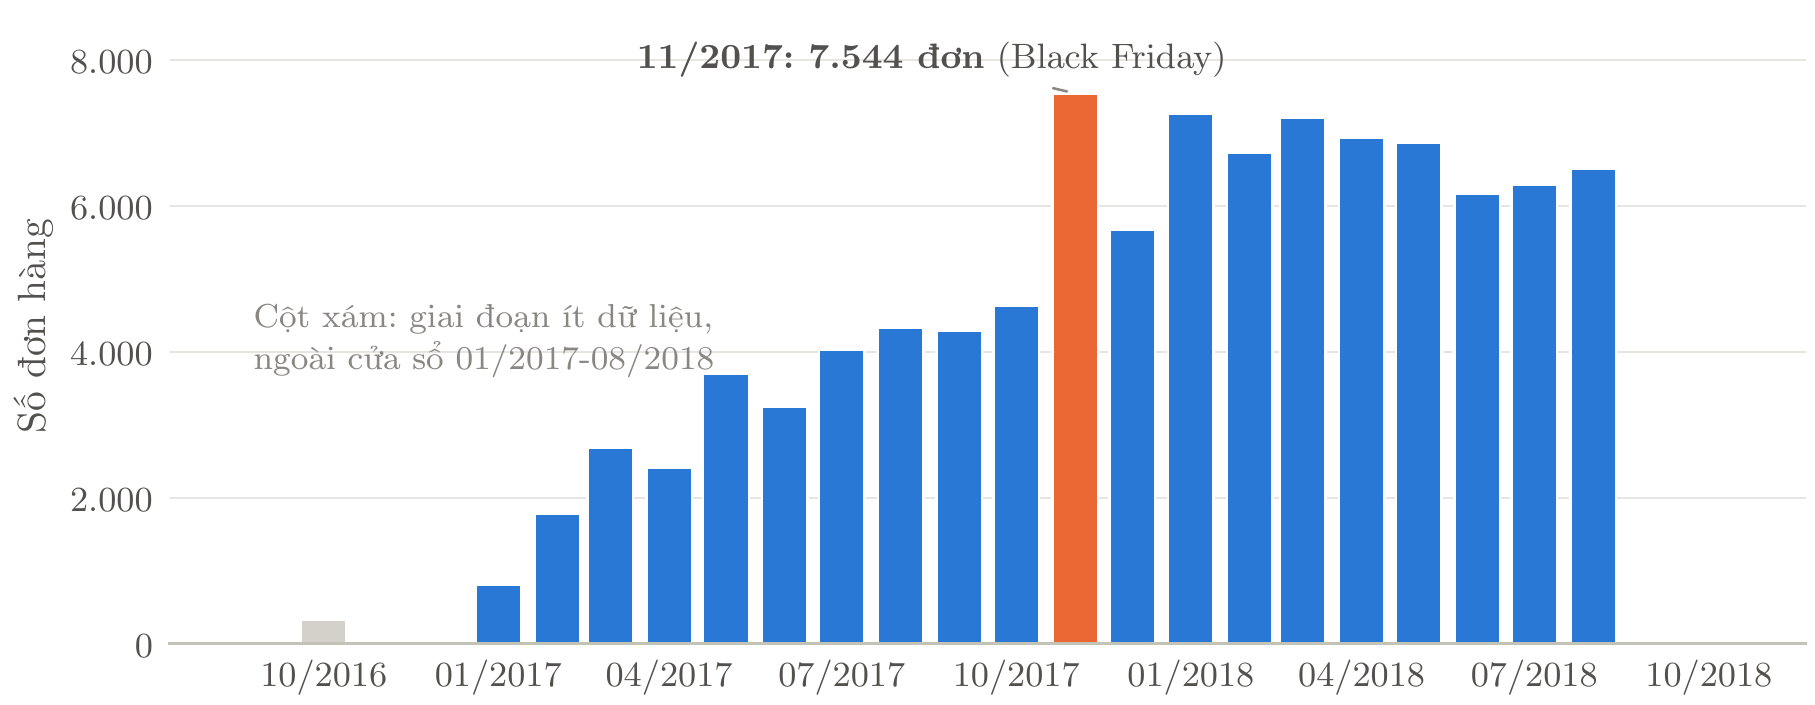
\includegraphics{Pictures/fig-don-hang-theo-thang.png}
\caption{Số đơn hàng theo tháng đặt hàng (tháng 09/2016 đến tháng 10/2018)}
\label{fig:donhangthang}
\end{figure}

\subsubsection{Quan hệ giữa các tập dữ liệu}\label{sec:quanhe}

Các tập dữ liệu liên kết với nhau qua khóa như trong Bảng~\ref{tab:quanhe} và Hình~\ref{fig:quanhe-nguon}. Bảng \code{orders} là trung tâm: mọi tập còn lại đều nối về đơn hàng, trực tiếp hoặc qua \code{order\_items}.

\begingroup\small\setstretch{1.1}
\begin{longtable}{|p{2.8cm}|p{4.1cm}|p{4.3cm}|l|}
\caption{Quan hệ giữa các tập dữ liệu nguồn}\label{tab:quanhe}\\
\hline
\textbf{Tập dữ liệu} & \textbf{Liên kết với} & \textbf{Khóa} & \textbf{Quan hệ}\\ \hline \endfirsthead
\hline
\textbf{Tập dữ liệu} & \textbf{Liên kết với} & \textbf{Khóa} & \textbf{Quan hệ}\\ \hline \endhead
\code{orders} & \code{customers} & \code{customer\_id} & 1 -- 1\\ \hline
\code{orders} & \code{order\_items} & \code{order\_id} & 1 -- nhiều\\ \hline
\code{orders} & \code{order\_payments} & \code{order\_id} & 1 -- nhiều\\ \hline
\code{orders} & \code{order\_reviews} & \code{order\_id} & 1 -- nhiều\\ \hline
\code{order\_items} & \code{products} & \code{product\_id} & nhiều -- 1\\ \hline
\code{order\_items} & \code{sellers} & \code{seller\_id} & nhiều -- 1\\ \hline
\code{customers}, \code{sellers} & \code{geolocation} & tiền tố mã bưu chính & nhiều -- nhiều\\ \hline
\code{products} & \code{category\_translation} & \code{product\_category\_name} & nhiều -- 1\\ \hline
\end{longtable}
\endgroup

% % !TeX root = ../../main.tex
% Quan hệ giữa 9 tập dữ liệu nguồn
\begin{figure}[H]
\centering
\begin{tikzpicture}[rel/.style={line width=0.6pt, draw=dwInkTwo, rounded corners=2pt},
                    geo/.style={line width=0.6pt, draw=dwYellow!80!black, dashed, rounded corners=2pt},
                    card/.style={font=\scriptsize, text=dwInkTwo},
                    end/.style={font=\scriptsize\bfseries, text=dwInk, fill=white, inner sep=1pt}]
\dwtable{orders}{0,0}{orders}{dwOrange}{2.7cm}{99.441 dòng, PK: order\_id}
\dwtable{items}{0,-2.4}{order\_items}{dwOrange}{2.7cm}{112.650 dòng, PK: order\_id + order\_item\_id}
\dwtable{customers}{-5.0,0}{customers}{dwBlue}{2.7cm}{99.441 dòng, PK: customer\_id}
\dwtable{payments}{5.2,0.75}{order\_payments}{dwBlue}{3.1cm}{103.886 dòng}
\dwtable{reviews}{5.2,-1.15}{order\_reviews}{dwBlue}{3.1cm}{99.224 dòng}
\dwtable{products}{-2.6,-4.9}{products}{dwBlue}{2.7cm}{32.951 dòng, PK: product\_id}
\dwtable{sellers}{2.6,-4.9}{sellers}{dwBlue}{2.7cm}{3.095 dòng, PK: seller\_id}
\dwtable{trans}{-2.6,-7.3}{category\_translation}{dwBlue}{3.9cm}{71 dòng}
\dwtable{geo}{-5.0,-2.4}{geolocation}{dwYellow}{2.7cm}{1.000.163 dòng, không có khóa}
% one-to-one / one-to-many
\draw[rel] (customers-1.east) -- node[end, pos=0.12] {1} node[end, pos=0.88] {1}
           node[font=\scriptsize\ttfamily, text=dwMuted, above=2pt, pos=0.5] {customer\_id} (orders-1.west);
\draw[rel] (orders-2.south) -- node[end, pos=0.15] {1} node[end, pos=0.75] {n}
           node[font=\scriptsize\ttfamily, text=dwMuted, right=3pt, pos=0.45] {order\_id} (items.north);
\draw[rel] (orders-1.east) -- ++(0.55,0) |- node[end, pos=0.92] {n} (payments.west);
\draw[rel] (orders-1.east) -- ++(0.55,0) |- node[end, pos=0.92] {n} (reviews.west);
\node[end] at ($(orders-1.east)+(0.25,0)$) {1};
\draw[rel] (items-2.south) -- ++(0,-0.35) -| node[end, pos=0.9] {1} (products.north);
\draw[rel] (items-2.south) -- ++(0,-0.35) -| node[end, pos=0.9] {1} (sellers.north);
\node[end] at ($(items-2.south)+(0,-0.2)$) {n};
\node[font=\scriptsize\ttfamily, text=dwMuted, anchor=south] at ($(items-2.south)+(-1.45,-0.35)$) {product\_id};
\node[font=\scriptsize\ttfamily, text=dwMuted, anchor=south] at ($(items-2.south)+(1.4,-0.35)$) {seller\_id};
\draw[rel] (products-2.south) -- node[end, pos=0.2] {n} node[end, pos=0.8] {1} (trans.north);
% zip prefix links (no unique key)
\draw[geo] (geo.north) -- node[font=\scriptsize, text=dwYellow!70!black, fill=white, inner sep=1pt] {mã bưu chính} (customers-2.south);
\draw[geo] (geo-2.south) -- ++(0,-2.95) -| node[font=\scriptsize, text=dwYellow!70!black, fill=white, inner sep=1pt, pos=0.25] {mã bưu chính} (sellers-2.south);
% legend
\node[font=\scriptsize, text=dwInkTwo, align=left, anchor=north west] at (0.2,-6.75)
  {\textcolor{dwOrange}{\rule{6pt}{6pt}} bảng trung tâm của đơn hàng\\[1pt]
   \textcolor{dwYellow}{\rule{6pt}{6pt}} dữ liệu địa lý, nối qua mã bưu chính\\[1pt]
   \textbf{1}, \textbf{n}: số dòng ở mỗi đầu quan hệ};
\end{tikzpicture}
\caption{Quan hệ giữa các tập dữ liệu nguồn (nét đứt: liên kết qua tiền tố mã bưu chính, không có khóa duy nhất)}
\label{fig:quanhenguon}
\end{figure}


\begin{figure}[H]
\centering
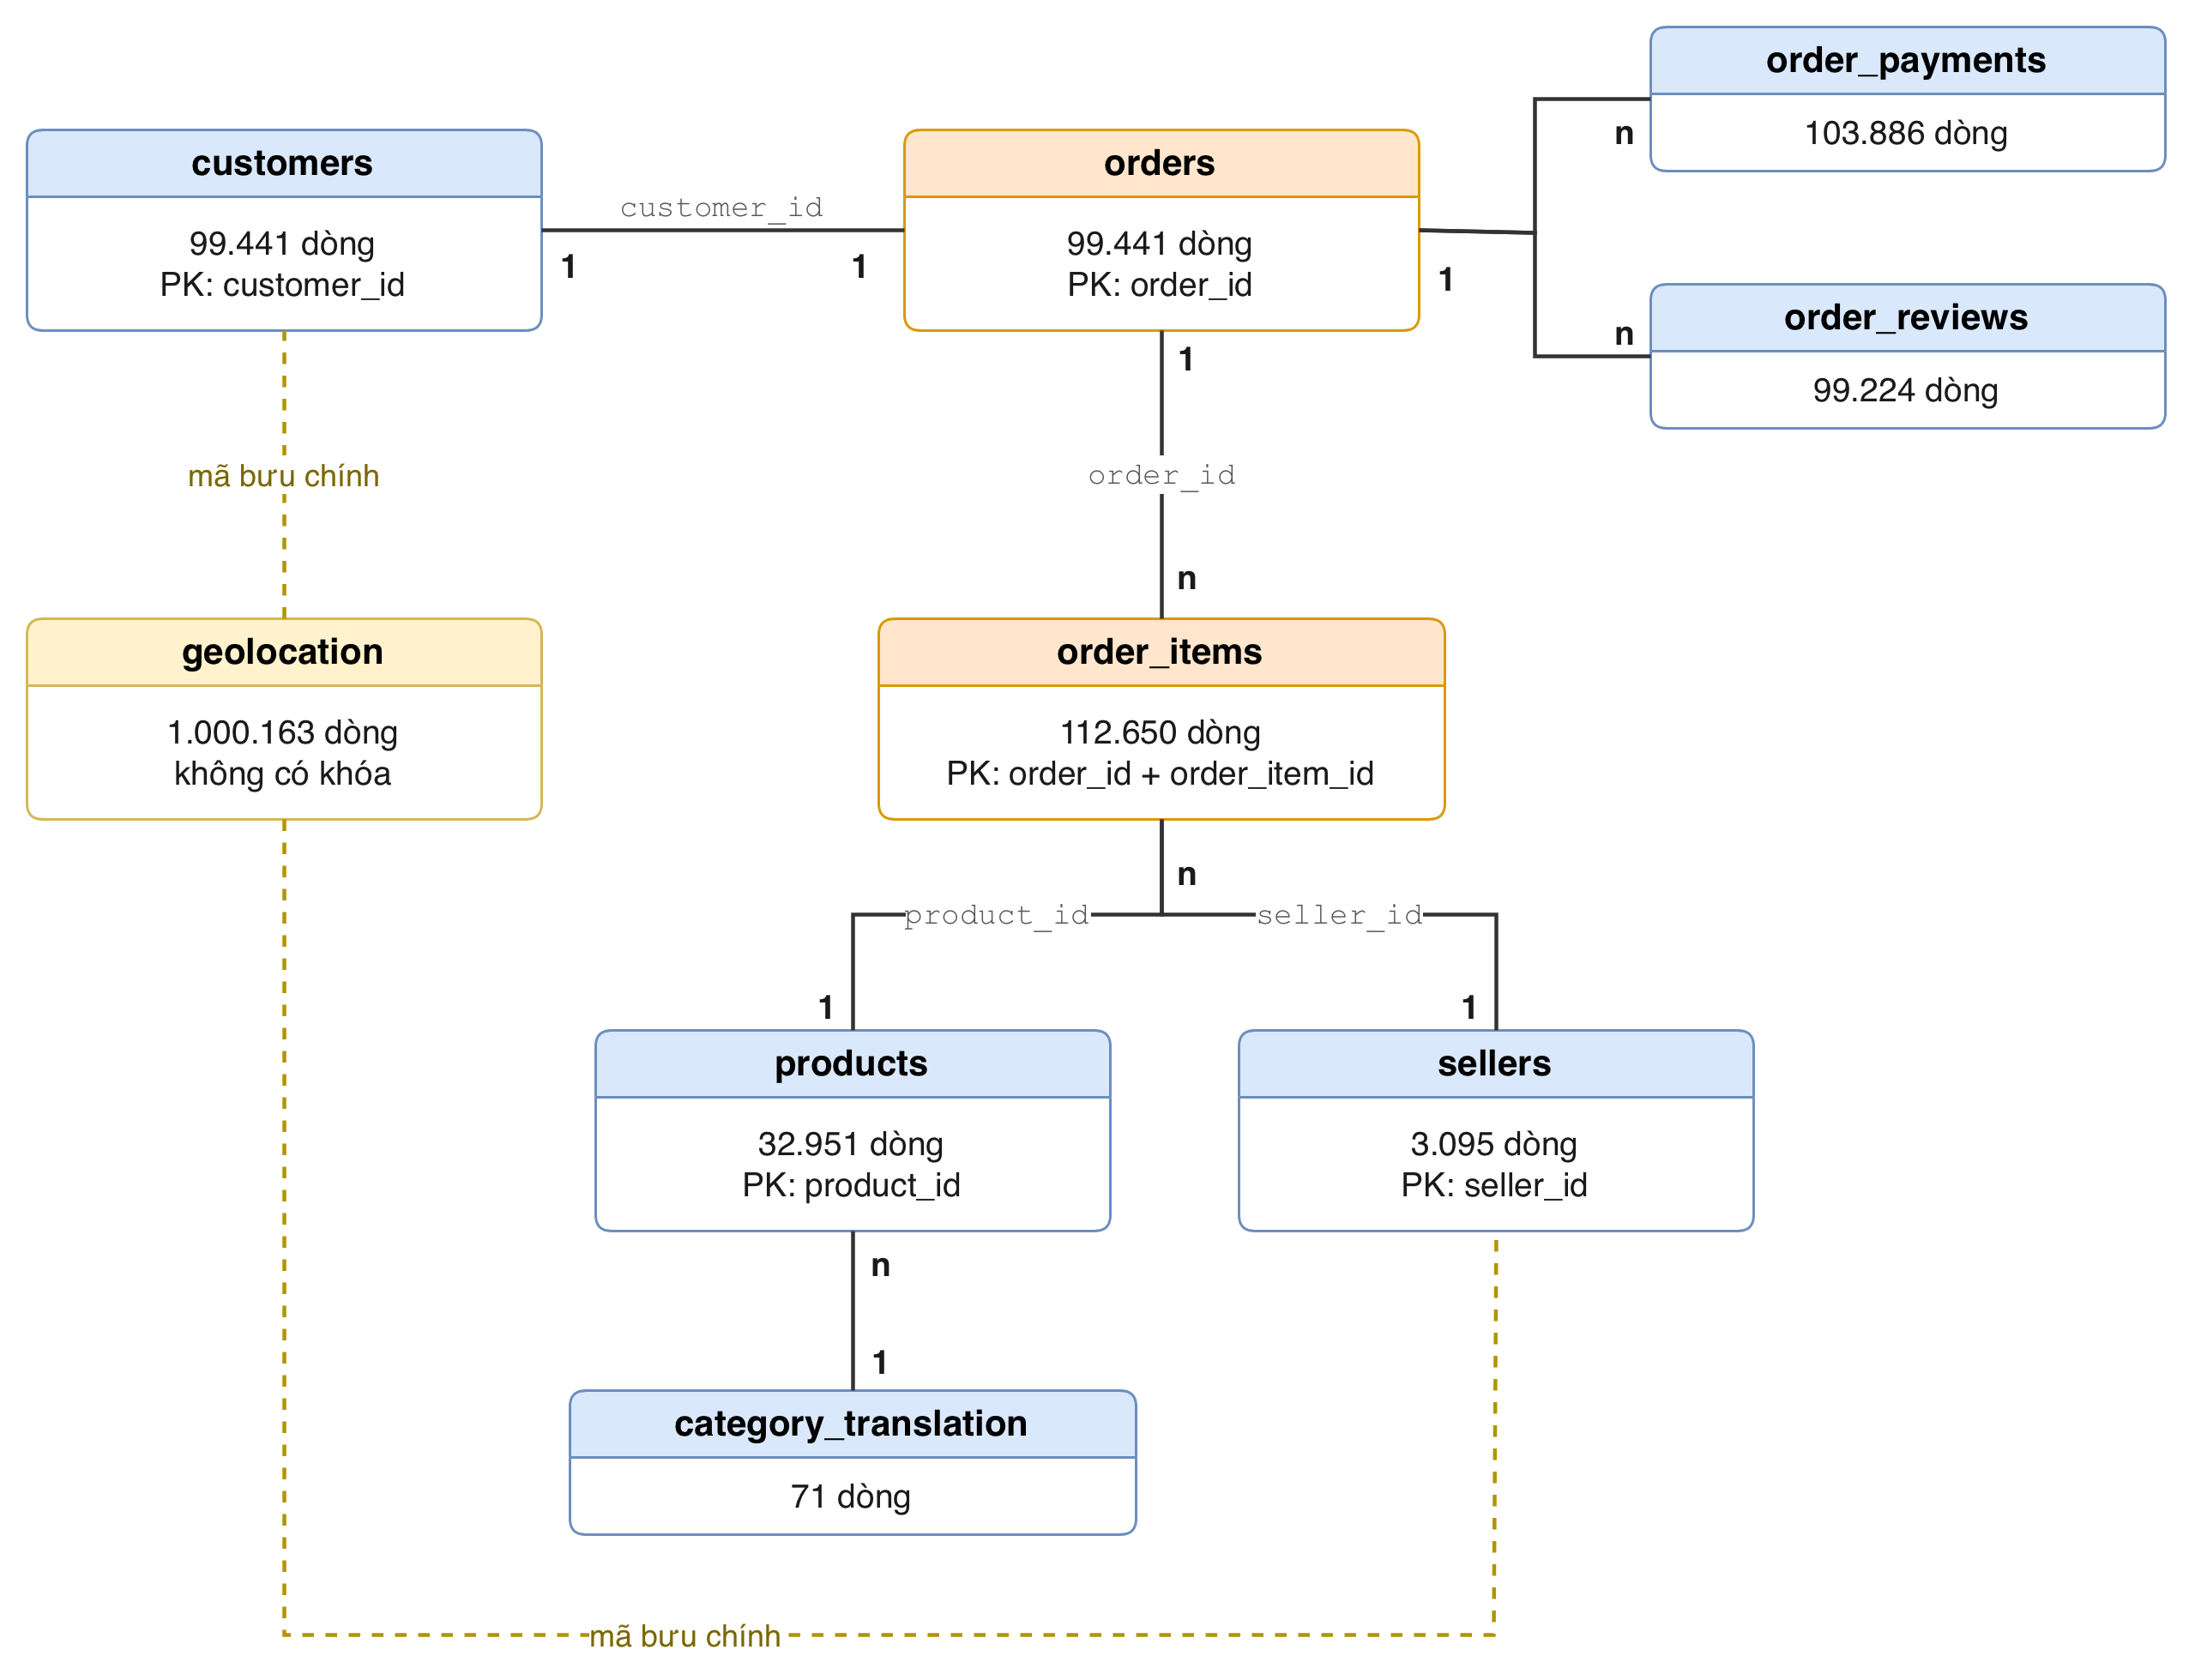
\includegraphics[width=\linewidth]{Pictures/quanhe_nguon.png}
\caption{Sơ đồ quan hệ giữa các tập dữ liệu nguồn}
\label{fig:quanhe-nguon}
\end{figure}


Các quan hệ này có ba đặc điểm ảnh hưởng trực tiếp đến thiết kế kho dữ liệu: 
\begin{enumerate}
    \item Dữ liệu không cùng mức chi tiết: giá, phí vận chuyển và người bán được ghi theo từng dòng sản phẩm, còn thanh toán, đánh giá và các mốc giao hàng được ghi theo đơn hàng.
    \item \code{customer\_id} được sinh mới cho mỗi đơn hàng, nên không thể dùng nó để đếm khách hàng. Mã nhận diện khách hàng thật là \code{customer\_unique\_id}, với 96.096 giá trị, trong đó 2.997 khách hàng có từ hai \code{customer\_id} trở lên. 
    \item Tập \code{geolocation} không có khóa duy nhất: một tiền tố mã bưu chính ứng với nhiều dòng tọa độ, nên phải gom lại trước khi nối với khách hàng và người bán.
\end{enumerate}
Phân bố của từng thuộc tính, các giá trị thiếu, ngoại lai và lỗi dữ liệu được khảo sát chi tiết ở mục~\ref{sec:eda}, cùng với các quy tắc tiền xử lý rút ra từ đó.


\clearpage
% !TeX root = ../main.tex
\section{Khám phá và tiền xử lý dữ liệu}\label{sec:eda}

Phần này gồm ba bước: khám phá dữ liệu thô (Exploratory Data Analysis -- EDA), đặt quy tắc tiền xử lý, rồi khám phá lại dữ liệu sau xử lý. Dữ liệu thô được khảo sát trực tiếp trên chín tập tin CSV bằng \code{src/eda/run\_eda.py}, độc lập với ETL, nên các con số ở đây cũng dùng để đối soát kết quả ETL ở mục~\ref{sec:hienthuc}. Dữ liệu sau tiền xử lý được nạp vào Data Mart gồm bảng fact \code{fact\_sales}, mỗi dòng ứng với một sản phẩm trong một đơn hàng, và 7 bảng chiều (thiết kế chi tiết ở mục~\ref{sec:thietke}); bản ghi nào không được nạp vào bảng fact thì không được tính vào các chỉ số của kho.

\subsection{Khám phá dữ liệu thô}\label{sec:edatho}

\subsubsection{Cấu trúc các tập dữ liệu}

Bảng~\ref{tab:cautruc} tóm tắt cấu trúc của chín tập tin: tổng cộng 52 cột. Bốn tập \code{order\_items}, \code{order\_payments}, \code{customers} và \code{sellers} không thiếu giá trị nào và không có dòng trùng. Giá trị thiếu tập trung ở ba tập \code{orders}, \code{order\_reviews} và \code{products}; dòng trùng chỉ xuất hiện ở \code{geolocation}.

\begin{table}[H]
\centering
\small\setstretch{1.1}
\caption{Cấu trúc, giá trị thiếu và dòng trùng của các tập dữ liệu thô}
\label{tab:cautruc}
\begin{tabularx}{\linewidth}{|>{\raggedright\arraybackslash}X|P{1.8cm}|P{1.2cm}|P{1.6cm}|P{1.8cm}|P{1.5cm}|}
\hline
\textbf{Tập tin} & \textbf{Số dòng} & \textbf{Số cột} & \textbf{Ô bị thiếu} & \textbf{Dòng có ô thiếu} & \textbf{Dòng trùng}\\ \hline
\textcolor{red}{\code{orders}} & \textcolor{red}{99.441} & \textcolor{red}{8} & \textcolor{red}{4.908} & \textcolor{red}{2.980} & \textcolor{red}{0}\\ \hline
\code{order\_items} & 112.650 & 7 & 0 & 0 & 0\\ \hline
\code{order\_payments} & 103.886 & 5 & 0 & 0 & 0\\ \hline
\textcolor{red}{\code{order\_reviews}} & \textcolor{red}{99.224} & \textcolor{red}{7} & \textcolor{red}{145.903} & \textcolor{red}{89.385} & \textcolor{red}{0}\\ \hline
\code{customers} & 99.441 & 5 & 0 & 0 & 0\\ \hline
\code{sellers} & 3.095 & 4 & 0 & 0 & 0\\ \hline
\textcolor{red}{\code{products}} & \textcolor{red}{32.951} & \textcolor{red}{9} & \textcolor{red}{2.448} & \textcolor{red}{611} & \textcolor{red}{0}\\ \hline
\textcolor{red}{\code{geolocation}} & \textcolor{red}{1.000.163} & \textcolor{red}{5} & \textcolor{red}{0} & \textcolor{red}{0} & \textcolor{red}{261.831}\\ \hline
\code{category\_translation} & 71 & 2 & 0 & 0 & 0\\ \hline
\end{tabularx}
\end{table}

\subsubsection{Phân tích giá trị thiếu}

Hình~\ref{fig:giatrithieu} cho thấy số dòng và tỷ lệ thiếu của từng cột trong 13 cột có giá trị thiếu, thuộc ba tập \code{order\_reviews}, \code{orders} và \code{products}. Hai cột thiếu nhiều nhất là tiêu đề và nội dung bình luận đánh giá, lần lượt 88,3\% và 58,7\%. Đây không phải lỗi: khách chỉ chấm sao mà không viết gì là chuyện bình thường. Tuy vậy, trong các đánh giá có viết bình luận, 26,6\% là đánh giá 1-2 sao, còn trong các đánh giá không có bình luận, tỷ lệ này chỉ là 6,3\%. Nói cách khác, khách thường viết bình luận khi không hài lòng.

\begin{figure}[H]
\centering
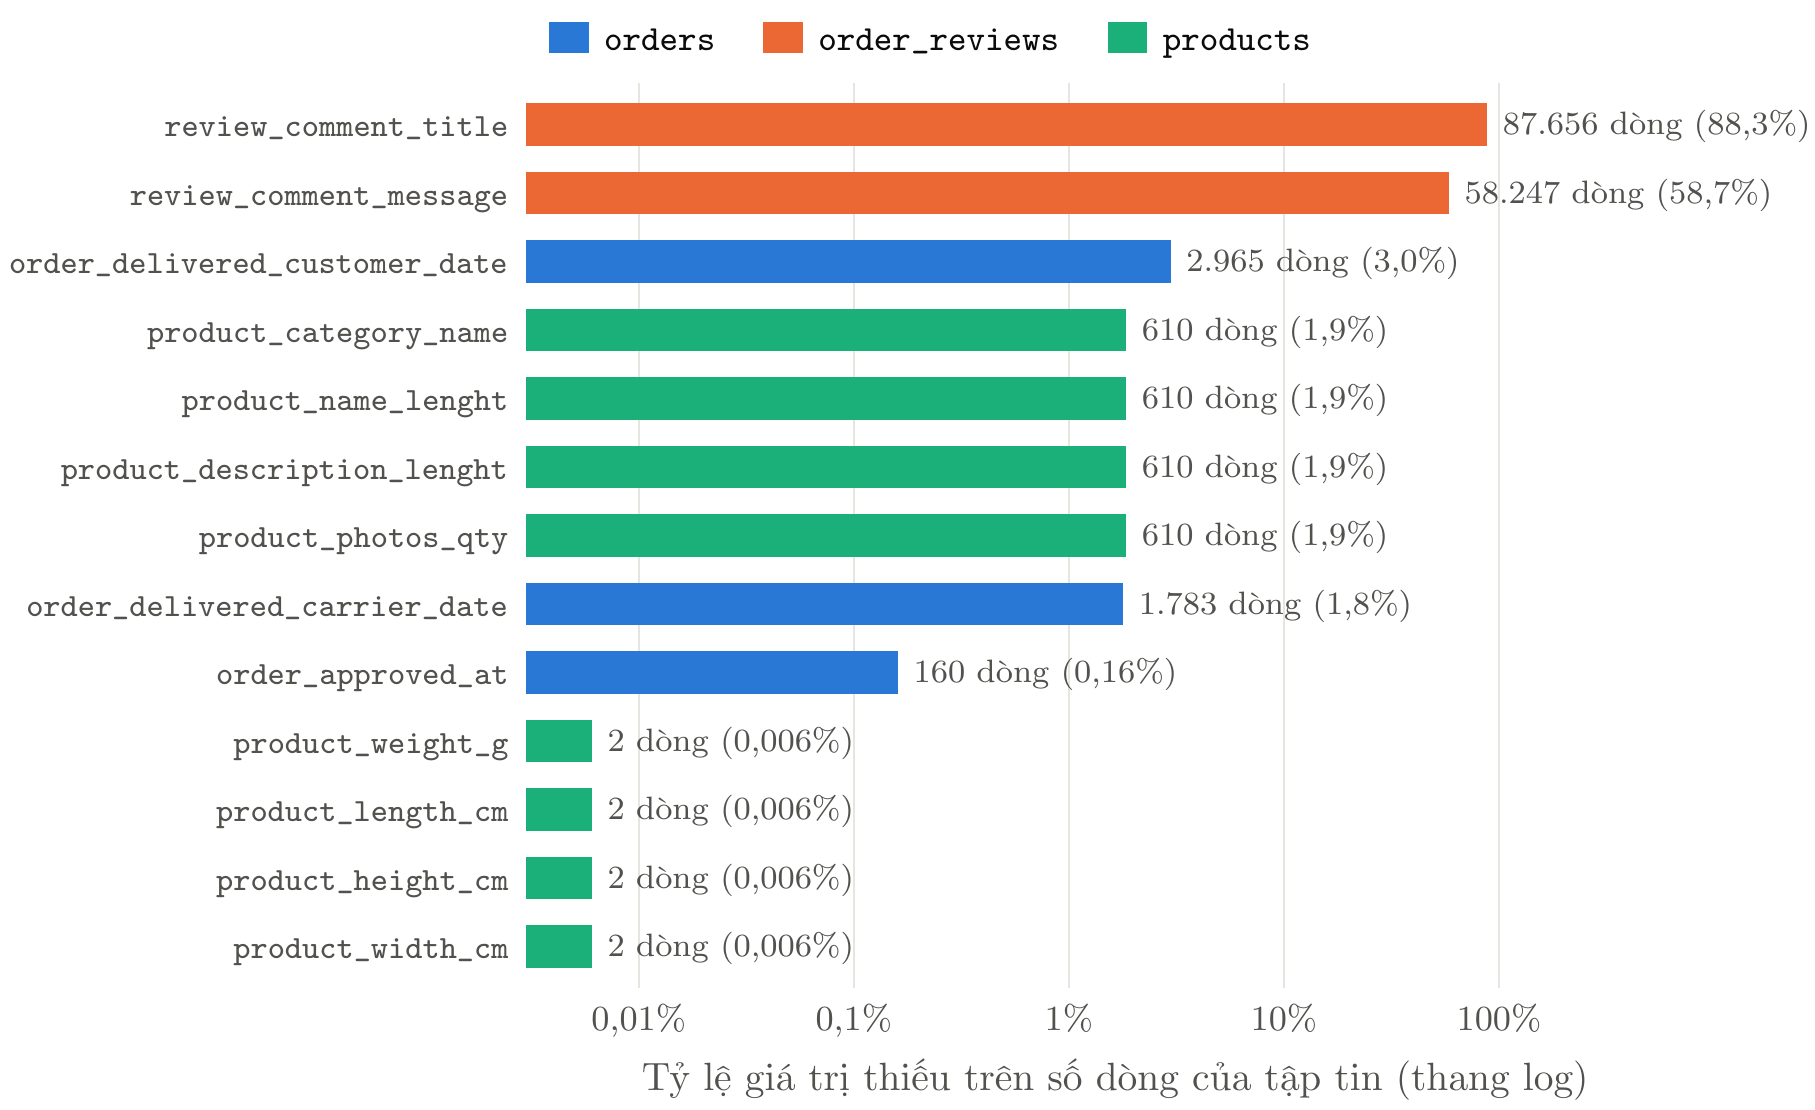
\includegraphics{Pictures/fig-eda-gia-tri-thieu.png}
\caption{Số dòng và tỷ lệ giá trị thiếu của từng cột trong dữ liệu thô (trục ngang theo thang log)}
\label{fig:giatrithieu}
\end{figure}

Ba cột mốc thời gian của \code{orders} thiếu ít hơn nhiều, và phần lớn trường hợp thiếu đều có lý do nghiệp vụ:
\begin{itemize}
    \item Ngày khách nhận hàng thiếu ở 2.965 đơn. Trong đó 2.957 đơn chưa từng được giao (đang vận chuyển, bị hủy hoặc hết hàng), chỉ có 8 đơn ở trạng thái \code{delivered} nhưng không ghi ngày nhận.
    \item Ngày bàn giao cho đơn vị vận chuyển thiếu ở 1.783 đơn, trong đó 1.781 đơn thực sự chưa được bàn giao.
    \item Thời điểm duyệt đơn thiếu ở 160 đơn, trong đó 141 đơn đã bị hủy.
\end{itemize}
Ba cột này thường thiếu cùng lúc trên một đơn: 1.782 trong 1.783 đơn thiếu ngày bàn giao cũng thiếu ngày nhận, và 146 đơn thiếu cả ba mốc. Vì thế 4.908 ô thiếu chỉ rơi vào 2.980 đơn. Với các cột này, nhóm không điền giá trị thay thế như trung bình, vì một đơn đã hủy thì không có ngày giao hàng.

Tập \code{products} cũng có hiện tượng tương tự, giá trị thiếu chia thành hai nhóm cột:
\begin{itemize}
    \item nhóm thông tin mô tả (\code{product\_category\_name}, \code{product\_name\_lenght}, \code{product\_description\_lenght}, \code{product\_photos\_qty}) cùng thiếu ở đúng 610 sản phẩm;
    \item nhóm kích thước và khối lượng (\code{product\_weight\_g}, \code{product\_length\_cm}, \code{product\_height\_cm}, \code{product\_width\_cm}) cùng thiếu ở đúng 2 sản phẩm.
\end{itemize}
Có 1 sản phẩm thiếu cả hai nhóm, nên 2.448 ô thiếu chỉ nằm trên 611 dòng. Đây là những sản phẩm được người bán đăng thiếu thông tin ngay từ đầu, không phải lỗi rải rác trong dữ liệu.

\subsubsection{Phát hiện giá trị ngoại lai}

Ngoại lai của bốn thước đo số chính được xác định bằng quy tắc khoảng tứ phân vị (IQR): một giá trị là ngoại lai nếu lớn hơn $Q_3 + 1{,}5 \times (Q_3 - Q_1)$. Hình~\ref{fig:ngoailai} cho thấy cả bốn thước đo đều lệch phải mạnh. Giá bán có trung vị 74,99 BRL nhưng 8.427 dòng (7,5\%) vượt ngưỡng 277,40 BRL, cao nhất là 6.735 BRL; thời gian giao hàng có trung vị 10,2 ngày, 4.899 đơn (5,1\%) vượt ngưỡng 29,2 ngày, lâu nhất là 209,6 ngày.

\begin{figure}[H]
\centering
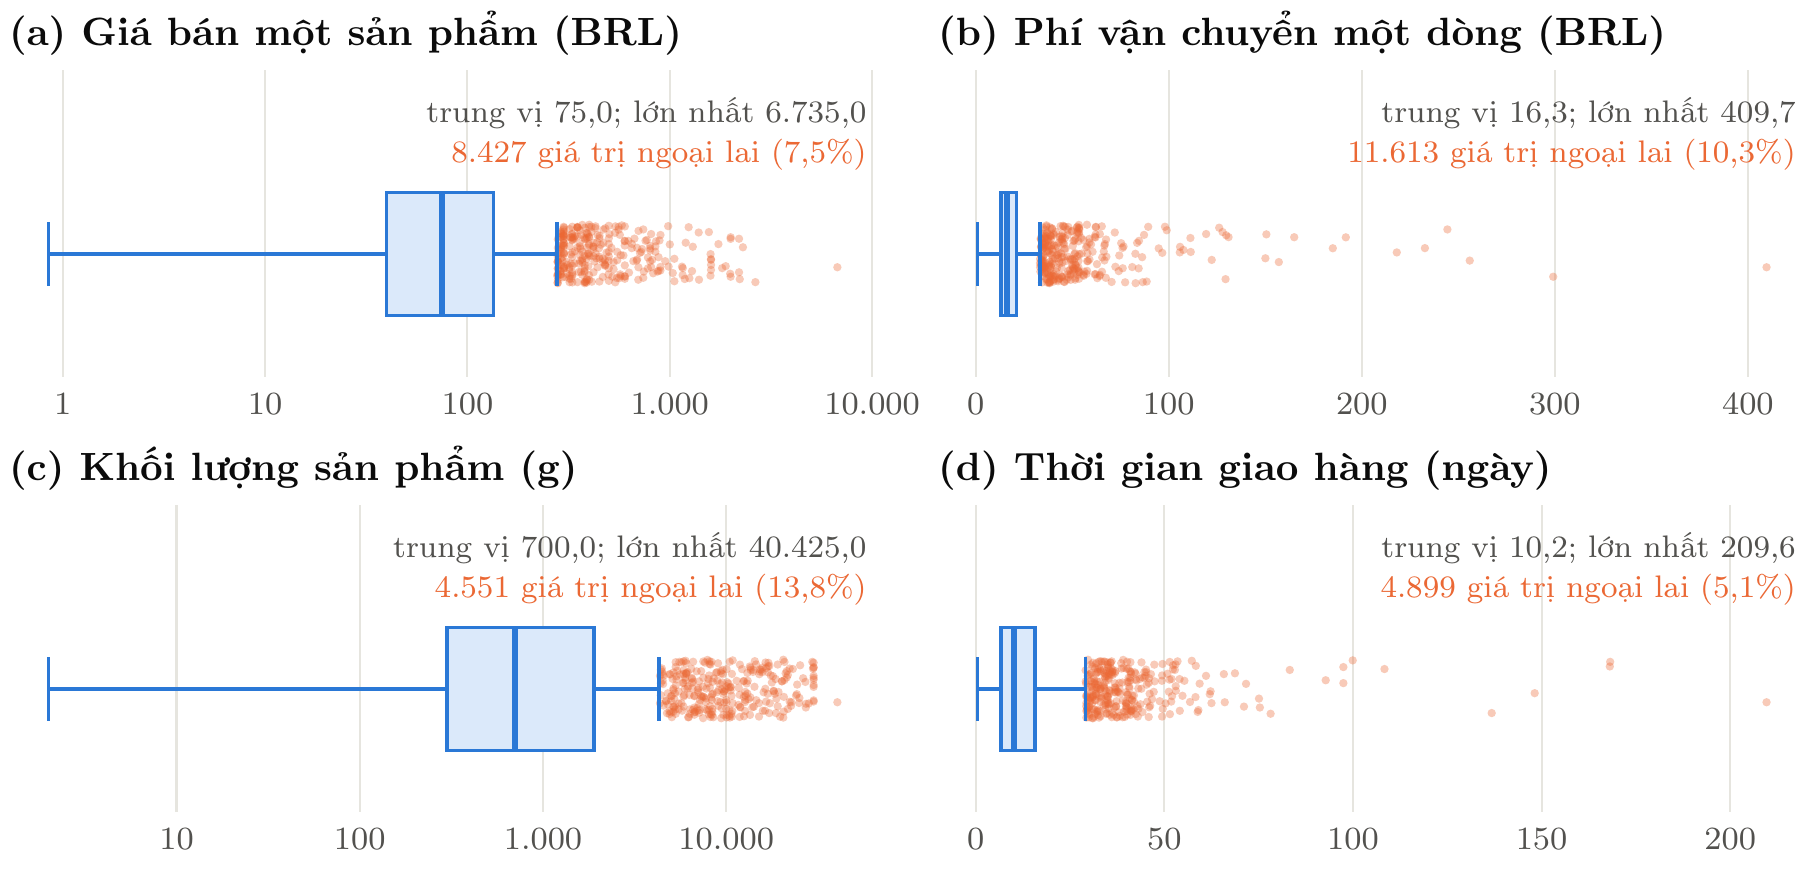
\includegraphics{Pictures/fig-eda-ngoai-lai.png}
\caption{Phân bố và giá trị ngoại lai (theo quy tắc IQR) của bốn thước đo số; điểm cam là một mẫu 300 giá trị ngoại lai, số đếm tính trên toàn bộ dữ liệu}
\label{fig:ngoailai}
\end{figure}

Các giá trị ngoại lai này được \textit{giữ lại} vì cắt bớt sẽ làm sai tổng doanh thu, mà tổng doanh thu phải khớp với nguồn ở bước đối soát. Các giá trị thật sự vô lý chỉ có hai nhóm nhỏ: 4 sản phẩm có khối lượng bằng 0 và các mốc thời gian sai thứ tự, được xử lý riêng ở Bảng~\ref{tab:quytac}. Phí vận chuyển bằng 0 (383 dòng) cũng được giữ, vì đó là các đơn được miễn phí vận chuyển.

\subsubsection{Phân bố thời gian giao hàng và điểm đánh giá}

Với 96.470 đơn đã giao có đủ ngày nhận hàng, thời gian giao trung bình là 12,6 ngày nhưng trung vị chỉ 10,2 ngày (Hình~\ref{fig:thoigiangiao}a). Phần lớn đơn đến tay khách trong vòng hai tuần, nhưng có 4,7\% đơn mất hơn 30 ngày. Hình~\ref{fig:thoigiangiao}b so sánh ngày nhận hàng thực tế với ngày giao dự kiến mà sàn hứa với khách. Trung vị là 12 ngày \textit{trước} hạn, và 78,9\% đơn về sớm từ một tuần trở lên. Nói cách khác, sàn đặt ngày dự kiến khá rộng, nên phần lớn đơn đều đúng hạn. Chỉ 6,77\% đơn bị trễ, nhưng như sẽ thấy ở phần OLAP, nhóm đơn này ảnh hưởng rất mạnh đến điểm đánh giá.

\begin{figure}[H]
\centering
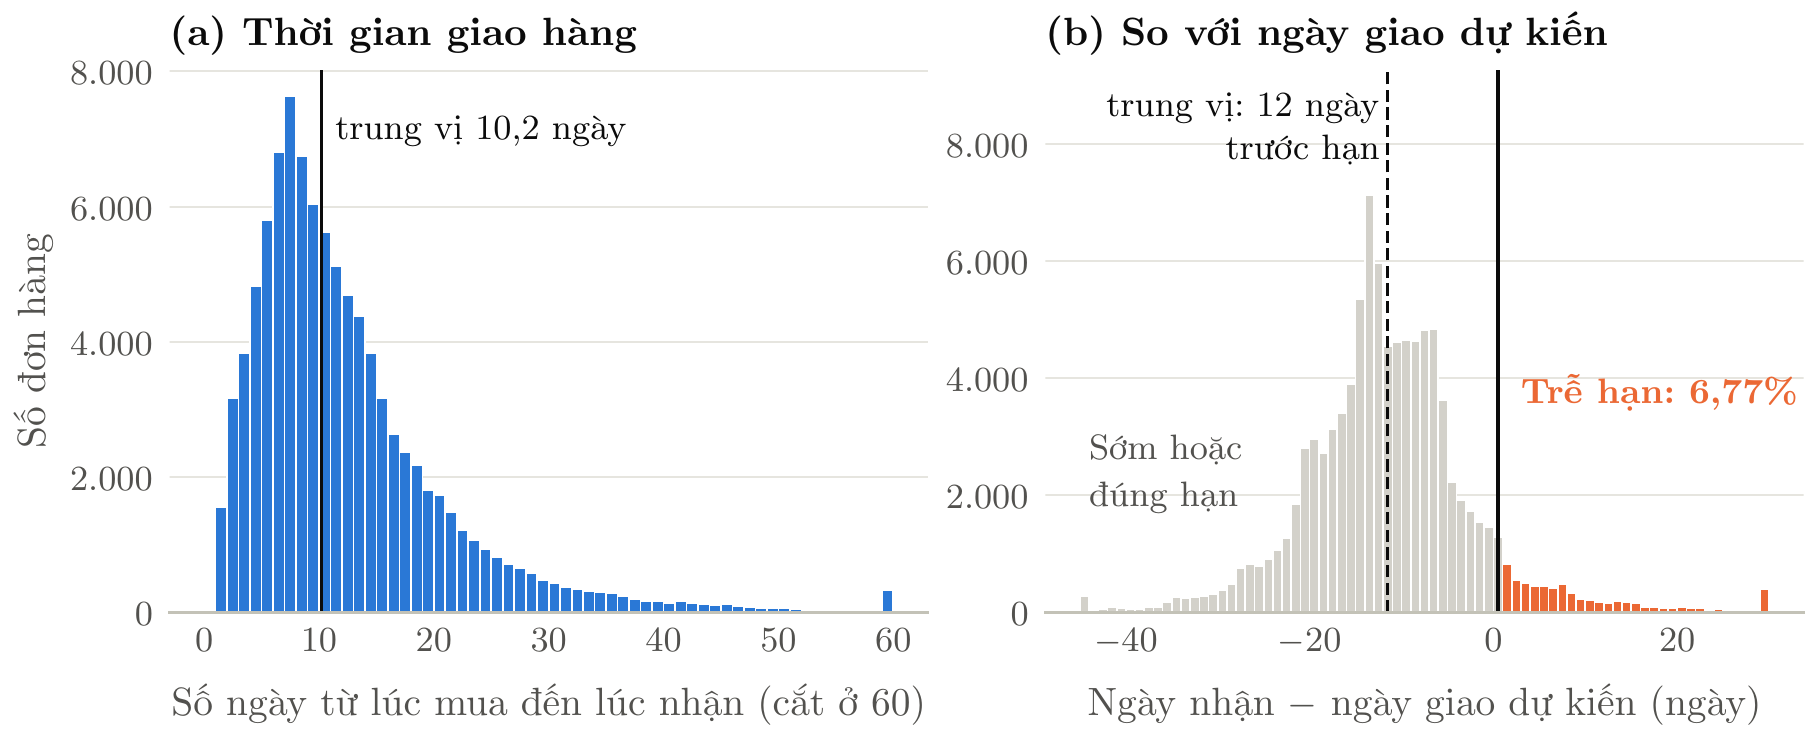
\includegraphics{Pictures/fig-thoi-gian-giao-hang.png}
\caption{Phân bố thời gian giao hàng (a) và chênh lệch giữa ngày nhận hàng với ngày giao dự kiến (b); màu cam là các đơn giao trễ}
\label{fig:thoigiangiao}
\end{figure}

Về đánh giá, sau khi giữ một đánh giá cho mỗi đơn hàng (cách chọn ở Bảng~\ref{tab:quytac}), có 98.673 đánh giá. Điểm phân cực rõ (Hình~\ref{fig:danhgia}): 57,8\% đánh giá là 5 sao, nhưng 1 sao lại chiếm 11,5\%, nhiều hơn cả 2 sao và 3 sao cộng lại. Điều này gợi ý rằng khách hàng thường chỉ chấm điểm thấp khi gặp một sự cố cụ thể, và giao trễ là thứ cần phải kiểm tra đầu tiên.

\begin{figure}[H]
\centering
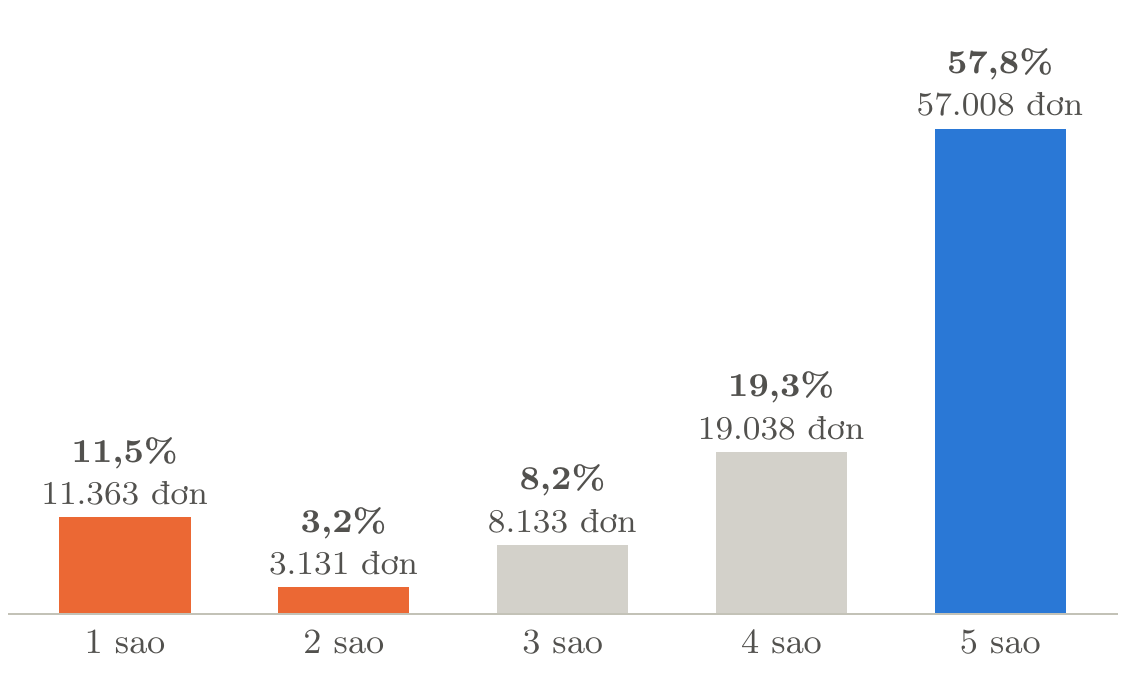
\includegraphics{Pictures/fig-phan-bo-danh-gia.png}
\caption{Phân bố điểm đánh giá của 98.673 đơn hàng (mỗi đơn một đánh giá)}
\label{fig:danhgia}
\end{figure}

\subsubsection{Tổng hợp các vấn đề chất lượng dữ liệu}

Ngoài giá trị thiếu và ngoại lai, dữ liệu còn được kiểm tra về tính duy nhất của khóa, thứ tự các mốc thời gian, tính nhất quán giữa các tập và cách viết tên địa danh. Bảng~\ref{tab:chatluong} liệt kê toàn bộ 31 vấn đề tìm được; đây là đầu vào trực tiếp cho bước tiền xử lý ở mục~\ref{sec:tienxuly}.

\begingroup\small\setstretch{1.1}
\begin{longtable}{|p{3.3cm}|p{8.2cm}|p{2.6cm}|}
\caption{Các vấn đề về chất lượng dữ liệu nguồn}\label{tab:chatluong}\\
\hline
\textbf{Tập dữ liệu} & \textbf{Vấn đề phát hiện} & \textbf{Số lượng}\\ \hline \endfirsthead
\hline
\textbf{Tập dữ liệu} & \textbf{Vấn đề phát hiện} & \textbf{Số lượng}\\ \hline \endhead
\code{orders} & Thiếu thời điểm duyệt đơn & 160 đơn\\ \hline
\code{orders} & Thiếu thời điểm bàn giao vận chuyển & 1.783 đơn\\ \hline
\code{orders} & Thiếu thời điểm khách nhận hàng & 2.965 đơn\\ \hline
\code{orders} & Trạng thái đã giao nhưng thiếu thời điểm nhận hàng & 8 đơn\\ \hline
\code{orders} & Thời điểm bàn giao vận chuyển sau thời điểm khách nhận hàng & 23 đơn\\ \hline
\code{orders} & Thời điểm bàn giao vận chuyển trước thời điểm duyệt đơn & 1.359 đơn\\ \hline
\code{orders} & Đơn hàng không có dòng sản phẩm & 775 đơn\\ \hline
\code{orders} & Đơn hàng không có dữ liệu thanh toán & 1 đơn\\ \hline
\code{orders} & Đơn hàng không có đánh giá & 768 đơn\\ \hline
\code{orders} & Giai đoạn đầu và cuối có rất ít dữ liệu (2016; 09-10/2018) & 349 đơn\\ \hline
\code{order\_items} & Phí vận chuyển bằng 0 & 383 dòng\\ \hline
\code{order\_payments} & Phương thức thanh toán không xác định (\code{not\_defined}) & 3 dòng\\ \hline
\code{order\_payments} & Giá trị thanh toán bằng 0 & 9 dòng\\ \hline
\code{order\_payments} & Số kỳ trả góp bằng 0 & 2 dòng\\ \hline
\code{order\_payments} & Tổng thanh toán lệch hơn 1 BRL (đồng Real Brazil) so với tiền hàng cộng phí vận chuyển & 249 đơn\\ \hline
\code{order\_reviews} & Một \code{review\_id} xuất hiện trên nhiều đơn hàng & 789 mã\\ \hline
\code{order\_reviews} & Một đơn hàng có nhiều đánh giá & 547 đơn\\ \hline
\code{order\_reviews} & Không có nội dung bình luận & 58,7\% số dòng\\ \hline
\code{order\_reviews} & Không có tiêu đề bình luận & 88,3\% số dòng\\ \hline
\code{products} & Thiếu ngành hàng và thông tin mô tả & 610 sản phẩm\\ \hline
\code{products} & Thiếu khối lượng và kích thước & 2 sản phẩm\\ \hline
\code{products} & Khối lượng bằng 0 & 4 sản phẩm\\ \hline
\code{products} & Sai chính tả tên cột (\code{product\_name\_lenght}, \code{product\_description\_lenght}) & 2 cột\\ \hline
\code{translation} & Ngành hàng chưa có bản dịch (\code{pc\_gamer} và một ngành hàng về dụng cụ nhà bếp) & 2 ngành hàng\\ \hline
\code{sellers} & Tên thành phố không chuẩn, ví dụ \code{sao paulo / sao paulo}, \code{sbc/sp}, \code{04482255} & 68 người bán\\ \hline
\code{sellers} & Mã bưu chính không có trong \code{geolocation} & 7 người bán\\ \hline
\code{customers} & Mã bưu chính không có trong \code{geolocation} & 278 khách hàng\\ \hline
\code{geolocation} & Dòng trùng lặp hoàn toàn & 261.831 dòng\\ \hline
\code{geolocation} & Tọa độ nằm ngoài lãnh thổ Brazil & 42 dòng\\ \hline
\code{geolocation} & Một mã bưu chính thuộc nhiều bang & 8 mã\\ \hline
\code{geolocation} & Một mã bưu chính ứng với nhiều cách viết tên thành phố & 8.556 mã\\ \hline
\end{longtable}
\endgroup

Các khóa chính của \code{orders} và \code{order\_items} đều toàn vẹn, nên phần lớn vấn đề nằm ở ba nhóm: giá trị thiếu, dữ liệu địa lý chưa chuẩn hóa, và mốc thời gian sai thứ tự. Dữ liệu địa lý là phần phải xử lý nhiều nhất. Khi vẽ toàn bộ tọa độ phân biệt lên mặt phẳng (Hình~\ref{fig:toado}a), 42 dòng (33 điểm phân biệt) rơi ra ngoài khung lãnh thổ Brazil, có điểm nằm ở châu Âu hoặc Bắc Mỹ. Nếu không loại các điểm này, tọa độ trung bình của thành phố sẽ bị kéo lệch hẳn. Phần còn lại (Hình~\ref{fig:toado}b) cho thấy khách hàng tập trung dày đặc ở vùng Đông Nam, quanh São Paulo và Rio de Janeiro. Từ đây, báo cáo ghi các bang bằng mã hai chữ cái như trong dữ liệu gốc (SP là São Paulo, RJ là Rio de Janeiro); danh sách đầy đủ 27 bang cùng vùng tương ứng nằm ở Bảng~\ref{tab:mabang} trong Phụ lục.

\begin{figure}[H]
\centering
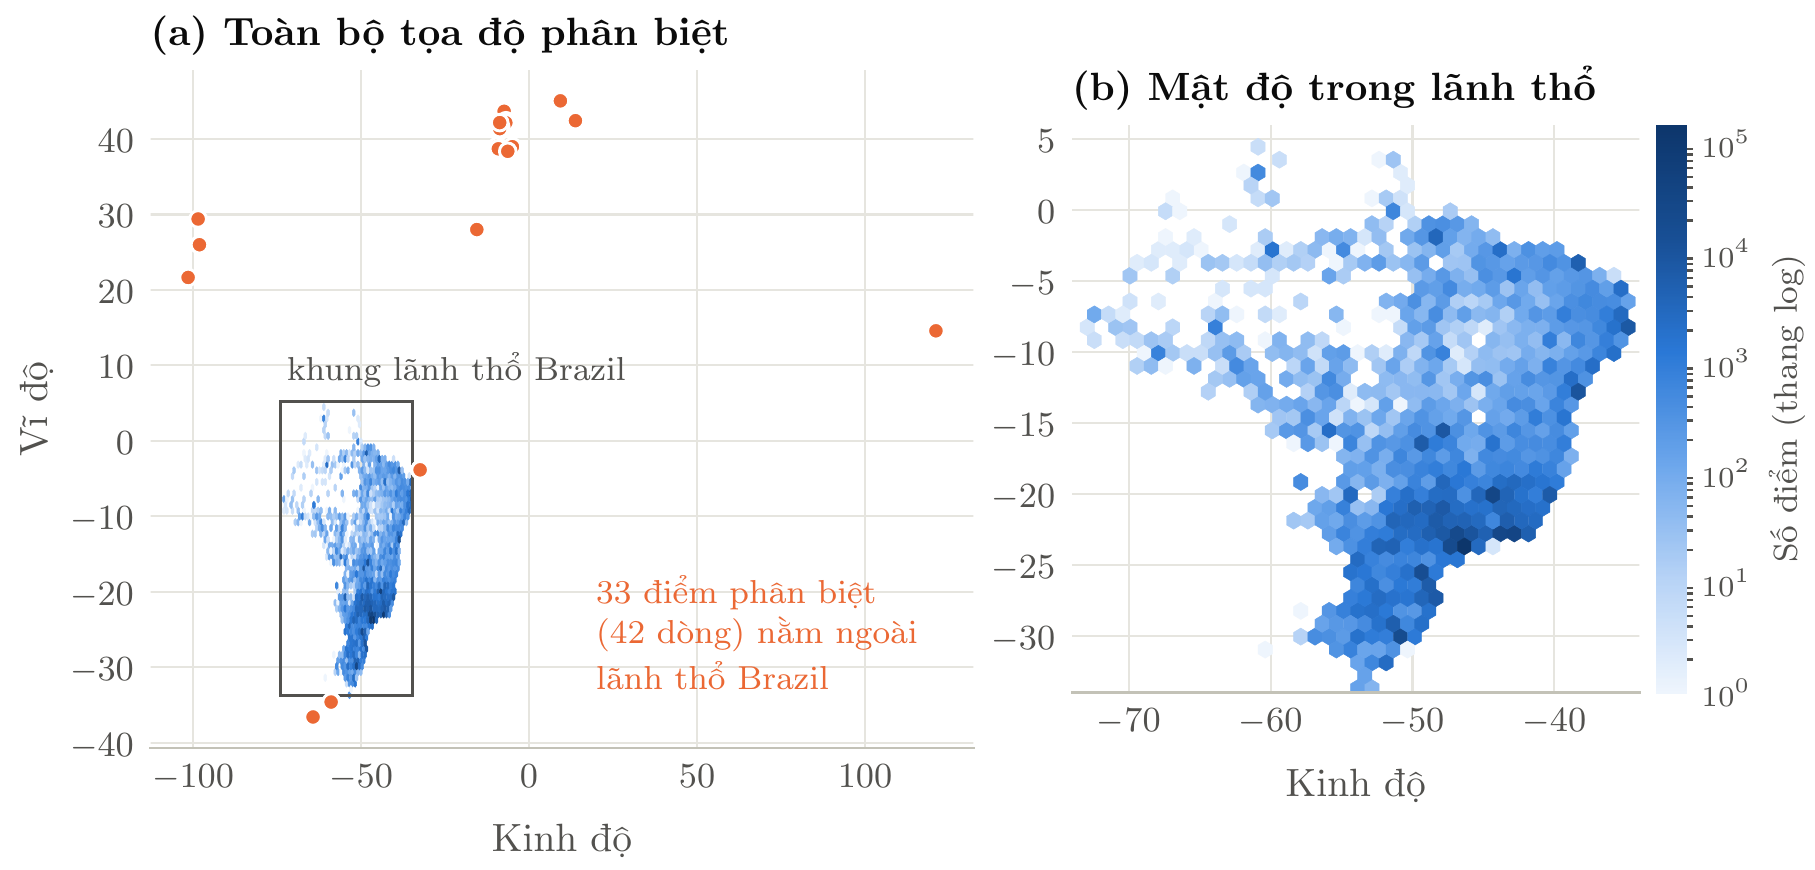
\includegraphics{Pictures/fig-toa-do-geolocation.png}
\caption{Tọa độ phân biệt trong tập \code{geolocation}: toàn bộ (a), khung chữ nhật là giới hạn lãnh thổ Brazil, và phần nằm trong lãnh thổ (b)}
\label{fig:toado}
\end{figure}
\subsection{Tiền xử lý dữ liệu}\label{sec:tienxuly}

Mỗi vấn đề ở Bảng~\ref{tab:chatluong} có một quy tắc xử lý riêng, được hiện thực ở bước transformation của quy trình ETL (mục~\ref{sec:thietke}); phần này chỉ nêu \textit{xử lý thế nào và vì sao}.

\subsubsection{Làm sạch dữ liệu}

Nguyên tắc chung là giữ lại càng nhiều dữ liệu hợp lệ càng tốt. Khi một mốc thời gian có vấn đề, chỉ thước đo liên quan bị để trống, còn đơn hàng vẫn được giữ; không có giá trị nào được điền bằng trung bình, vì như đã phân tích ở trên, phần lớn giá trị thiếu là thiếu có lý do. Bảng~\ref{tab:quytac} là quy tắc cho từng vấn đề ở Bảng~\ref{tab:chatluong}.

\begingroup\small\setstretch{1.1}
% Bảng rộng hơn khổ chữ: caption đặt ngoài longtable vì gói caption báo Overfull khi \LTleft âm
\captionof{table}{Quy tắc xử lý các vấn đề chất lượng dữ liệu}\label{tab:quytac}\nopagebreak
\setlength{\LTleft}{-1.2cm}\setlength{\LTright}{-0.6cm}\setlength{\LTpre}{4pt}
\begin{longtable}{|P{4.1cm}|P{5.6cm}|P{6.1cm}|}
\hline
\textbf{Vấn đề} & \textbf{Quy tắc xử lý} & \textbf{Ví dụ}\\ \hline \endfirsthead
\hline
\textbf{Vấn đề} & \textbf{Quy tắc xử lý} & \textbf{Ví dụ}\\ \hline \endhead
Đơn hàng thiếu thời điểm duyệt, bàn giao vận chuyển hoặc nhận hàng & Giữ lại đơn hàng. Cột ngày tương ứng được gán về bản ghi không xác định, các khoảng thời gian liên quan và cờ giao trễ để trống. & Đơn \code{1b9ecfe8\ldots} bị hủy, không có ngày bàn giao và ngày nhận $\rightarrow$ \code{carrier\_date\_key} và \code{delivered\_date\_key} bằng $-1$; \code{delivery\_days}, \code{is\_late} để trống.\\ \hline
Đơn hàng đã giao nhưng thiếu thời điểm nhận hàng (8 đơn) & Giữ lại, xử lý như đơn chưa có ngày nhận hàng và không tính vào các chỉ số giao hàng. & Đơn \code{2d1e2d5b\ldots} có trạng thái \code{delivered} nhưng ngày nhận trống $\rightarrow$ \code{delivered\_date\_key} bằng $-1$, \code{delivery\_days} để trống.\\ \hline
Thời điểm bàn giao vận chuyển sau thời điểm nhận hàng (23 đơn) & Giữ tổng thời gian giao hàng, để trống thời gian vận chuyển vì không xác định được thứ tự đúng. & Đơn \code{a1abeb65\ldots}: mua 20/7/2017, bàn giao 28/7/2017 nhưng nhận 25/7/2017 $\rightarrow$ \code{delivery\_days} = 5,34; \code{shipping\_days} để trống.\\ \hline
Thời điểm bàn giao vận chuyển trước thời điểm duyệt (1.359 đơn) & Giữ các mốc thời gian, để trống thời gian chuẩn bị hàng vì giá trị bị âm. & Đơn \code{dcb36b51\ldots}: duyệt lúc 23:31 ngày 12/6/2018 nhưng bàn giao lúc 14:54 ngày 11/6/2018 $\rightarrow$ \code{handling\_days} để trống.\\ \hline
Đơn hàng không có dòng sản phẩm (775 đơn) & Không nạp vào bảng fact, ghi nhận vào nhật ký ETL. & Đơn \code{e40d0c72\ldots} (trạng thái \code{unavailable}) không có dòng nào trong \code{order\_items} $\rightarrow$ không có trong \code{fact\_sales}.\\ \hline
Đơn hàng không có đánh giá (768 đơn) & Điểm đánh giá để trống, ngày đánh giá gán về bản ghi không xác định. & Đơn \code{01675428\ldots} $\rightarrow$ \code{review\_score} để trống, \code{review\_date\_key} bằng $-1$.\\ \hline
Đơn hàng có nhiều đánh giá (547 đơn) & Chọn đánh giá có thời điểm phản hồi muộn nhất làm đánh giá chính thức, vì đó là ý kiến cuối cùng của khách. Không lấy trung bình vì 202 đơn có các điểm khác nhau, trung bình sẽ tạo ra những điểm như 3,5 vốn không tồn tại. & Đơn \code{02355020\ldots} có đánh giá 3 sao (phản hồi 22/3/2018) và 1 sao (phản hồi 30/3/2018) $\rightarrow$ giữ đánh giá 1 sao.\\ \hline
Một \code{review\_id} xuất hiện trên nhiều đơn hàng (789 mã) & Không xử lý riêng, vì đánh giá được gắn vào bảng fact theo \code{order\_id}. & Mã \code{00130cbe\ldots} gắn với hai đơn \code{04a28263\ldots} và \code{dfcdfc43\ldots} $\rightarrow$ cả hai đơn đều nhận điểm 1 sao của đánh giá này.\\ \hline
Giá trị ngoại lai của giá, phí vận chuyển, khối lượng, thời gian giao & Giữ nguyên vì là giao dịch thật; phí vận chuyển bằng 0 (383 dòng) xem là miễn phí vận chuyển. & Dòng có giá 6.735 BRL của đơn \code{0812eb90\ldots} được giữ nguyên; đơn \code{079f1668\ldots} có phí vận chuyển 0 BRL cũng được giữ.\\ \hline
Sản phẩm thiếu ngành hàng (610 sản phẩm) & Gán vào ngành hàng ``không xác định''. & Sản phẩm \code{a41e356c\ldots} có ngành hàng trống $\rightarrow$ \code{unknown}.\\ \hline
Sản phẩm thiếu hoặc có khối lượng, kích thước bằng 0 (6 sản phẩm) & Để trống các thuộc tính này. & Sản phẩm \code{81781c0f\ldots} có khối lượng 0 g $\rightarrow$ \code{weight\_g} để trống, chiều dài 30 cm giữ nguyên.\\ \hline
Ngành hàng chưa có bản dịch (2 ngành hàng) & Bổ sung tên tiếng Anh thủ công vào bảng ngành hàng. & \code{portateis\_\allowbreak cozinha\_\allowbreak e\_\allowbreak preparadores\_\allowbreak de\_\allowbreak alimentos} $\rightarrow$ \code{portable\_\allowbreak kitchen\_\allowbreak food\_\allowbreak processors}.\\ \hline
Tên thành phố của người bán không chuẩn & Chuyển về chữ thường, bỏ dấu, bỏ phần mã bang thừa như ``/ sp'' hoặc ``- sp''. Nếu tên sau chuẩn hóa không có trong \code{geolocation} của bang tương ứng (ví dụ tên là chuỗi số, tên viết tắt hoặc viết sai chính tả) thì lấy tên thành phố theo mã bưu chính. & \code{auriflama/sp} $\rightarrow$ \code{auriflama}; \code{são paulo} $\rightarrow$ \code{sao paulo}. Tên \code{04482255} (mã bưu chính 22790) $\rightarrow$ \code{rio de janeiro}; \code{sbc} $\rightarrow$ \code{sao bernardo do campo}.\\ \hline
Dòng trùng lặp trong \code{geolocation} (261.831 dòng) & Loại bỏ, chỉ giữ lại 738.332 dòng phân biệt. & Mã bưu chính 24230 có 1.102 dòng nhưng chỉ 378 dòng khác nhau $\rightarrow$ giữ 378 dòng.\\ \hline
Tọa độ nằm ngoài lãnh thổ Brazil (42 dòng) & Loại bỏ trước khi tính tọa độ trung bình của thành phố. & Mã bưu chính 18243 (bang SP) có một dòng tọa độ (28,01; $-$15,54), nằm ngoài Brazil $\rightarrow$ loại dòng này.\\ \hline
Mã bưu chính thuộc nhiều bang (8 mã) & Chọn bang xuất hiện nhiều nhất để mỗi mã bưu chính tra ra đúng một bang trong bảng tra cứu; bang của khách hàng và người bán vẫn lấy từ dữ liệu gốc, không bị thay đổi. & Mã 02116 có 12 dòng ở bang SP và 1 dòng ở bang RN $\rightarrow$ bảng tra cứu ghi bang SP cho mã này.\\ \hline
Mã bưu chính không có trong \code{geolocation} (278 khách hàng, 7 người bán) & Vẫn lấy tên thành phố và bang từ bảng khách hàng hoặc người bán; tọa độ lấy theo thành phố nếu thành phố có trong \code{geolocation}, ngược lại để trống. & Khách hàng ở mã 72904 vẫn có tọa độ của thành phố \code{santo antonio do descoberto}; khách hàng ở mã 36956 giữ thành phố \code{sao francisco do humaita}, bang MG, nhưng vĩ độ, kinh độ để trống.\\ \hline
Các mã thanh toán bất thường (giá trị 0, phương thức không xác định) & Không ảnh hưởng đến phạm vi đề tài vì dữ liệu thanh toán không được nạp vào bảng fact; chỉ lưu lại trong khu vực staging. & --\\ \hline
\end{longtable}
\endgroup

\subsubsection{Chuẩn hóa, tích hợp và tạo thuộc tính mới}

Bên cạnh làm sạch, dữ liệu cần được đưa về cùng một dạng để các tập nối được với nhau. Kiểu dữ liệu được thống nhất: thời gian sang \code{timestamp}, tiền sang số thập phân, mã bưu chính giữ dạng chuỗi để không mất số 0 ở đầu. Mỗi khách hàng thật được nhận diện bằng \code{customer\_unique\_id} thay cho \code{customer\_id} sinh theo từng đơn. Tên thành phố của khách hàng và người bán được chuẩn hóa theo cùng một quy tắc rồi gộp thành một danh sách thành phố duy nhất, có tọa độ là trung bình các điểm \code{geolocation} hợp lệ.

Một số thuộc tính mới được tạo thêm để phục vụ phân tích. Bốn khoảng thời gian (duyệt đơn, chuẩn bị hàng, vận chuyển, tổng thời gian giao) được tính từ các mốc của đơn hàng; cờ giao trễ được tính bằng cách so ngày nhận hàng với ngày giao dự kiến. 27 bang được gom thành năm vùng địa lý, và mỗi ngày được tách thành tháng, quý, năm, thứ trong tuần, giống như cách rời rạc hóa (binning) một thuộc tính liên tục thành các nhóm để phân tích theo nhiều mức. Cách tính chi tiết của từng thuộc tính nằm ở phần thiết kế ETL.

\subsubsection{Kết quả tiền xử lý}

\begin{table}[H]
\centering
\small\setstretch{1.1}
\caption{Số lượng bản ghi trước và sau tiền xử lý}
\label{tab:truocsau}
\begin{tabularx}{\linewidth}{|>{\raggedright\arraybackslash}X|r|r|r|}
\hline
\textbf{Đối tượng} & \textbf{Dữ liệu thô} & \textbf{Sau làm sạch} & \textbf{Trong Data Mart}\\ \hline
Đơn hàng & 99.441 & 99.441 & 98.666\\ \hline
Dòng sản phẩm trong đơn & 112.650 & 112.650 & 112.650\\ \hline
Đánh giá & 99.224 & 98.673 & 97.917\\ \hline
Khách hàng (mã theo đơn $\rightarrow$ khách hàng thật) & 99.441 & 96.096 & 96.096\\ \hline
Sản phẩm & 32.951 & 32.951 & 32.951\\ \hline
Dòng tọa độ \code{geolocation} & 1.000.163 & 738.299 & --\\ \hline
Cách viết (thành phố, bang) của người bán & 636 & 580 & 580\\ \hline
Cách viết (thành phố, bang) của khách hàng & 4.310 & 4.301 & 4.301\\ \hline
Thành phố (khách hàng và người bán) & -- & 4.341 & 4.341\\ \hline
\end{tabularx}
\end{table}

Bảng~\ref{tab:truocsau} cho thấy tiền xử lý không làm mất bản ghi hợp lệ nào; mọi chênh lệch đều đến từ những chỗ có chủ đích:
\begin{itemize}
    \item Số đơn hàng trong Data Mart còn 98.666 vì 775 đơn không có dòng sản phẩm không được nạp vào bảng fact.
    \item Số đánh giá giảm từ 99.224 xuống 98.673 vì mỗi đơn chỉ giữ một đánh giá. Trong Data Mart còn 97.917 vì đánh giá của các đơn không có dòng sản phẩm cũng không vào bảng fact.
    \item 99.441 mã khách hàng theo đơn được gộp về 96.096 khách hàng thật theo \code{customer\_unique\_id}.
    \item Tập \code{geolocation} bỏ 261.831 dòng trùng (còn 738.332 dòng), rồi bỏ thêm 33 dòng có tọa độ nằm ngoài lãnh thổ Brazil, còn 738.299 dòng.
    \item Sau khi chuẩn hóa tên, 636 cách viết (thành phố, bang) của người bán được quy về 580 thành phố, 4.310 cách viết của khách hàng còn 4.301. Hợp hai danh sách này, thành phố xuất hiện ở cả hai chỉ tính một lần, được 4.341 thành phố.
\end{itemize}

\subsection{Khám phá dữ liệu sau tiền xử lý}\label{sec:edasach}

Sau khi làm sạch, dữ liệu được gom về mức đơn hàng (96.470 đơn đã giao) để khảo sát lại quan hệ giữa các thuộc tính và tìm những thuộc tính liên quan đến giao trễ, dùng cho phần OLAP và phần hỗ trợ quyết định.

\subsubsection{Tương quan giữa các thuộc tính}

Vì các thước đo lệch phải và có nhiều ngoại lai, hệ số tương quan hạng Spearman được dùng thay cho Pearson. Khoảng cách giữa thành phố người bán và thành phố khách được tính bằng công thức Haversine từ tọa độ đã làm sạch. Hình~\ref{fig:tuongquan} là ma trận tương quan.

\begin{figure}[H]
\centering
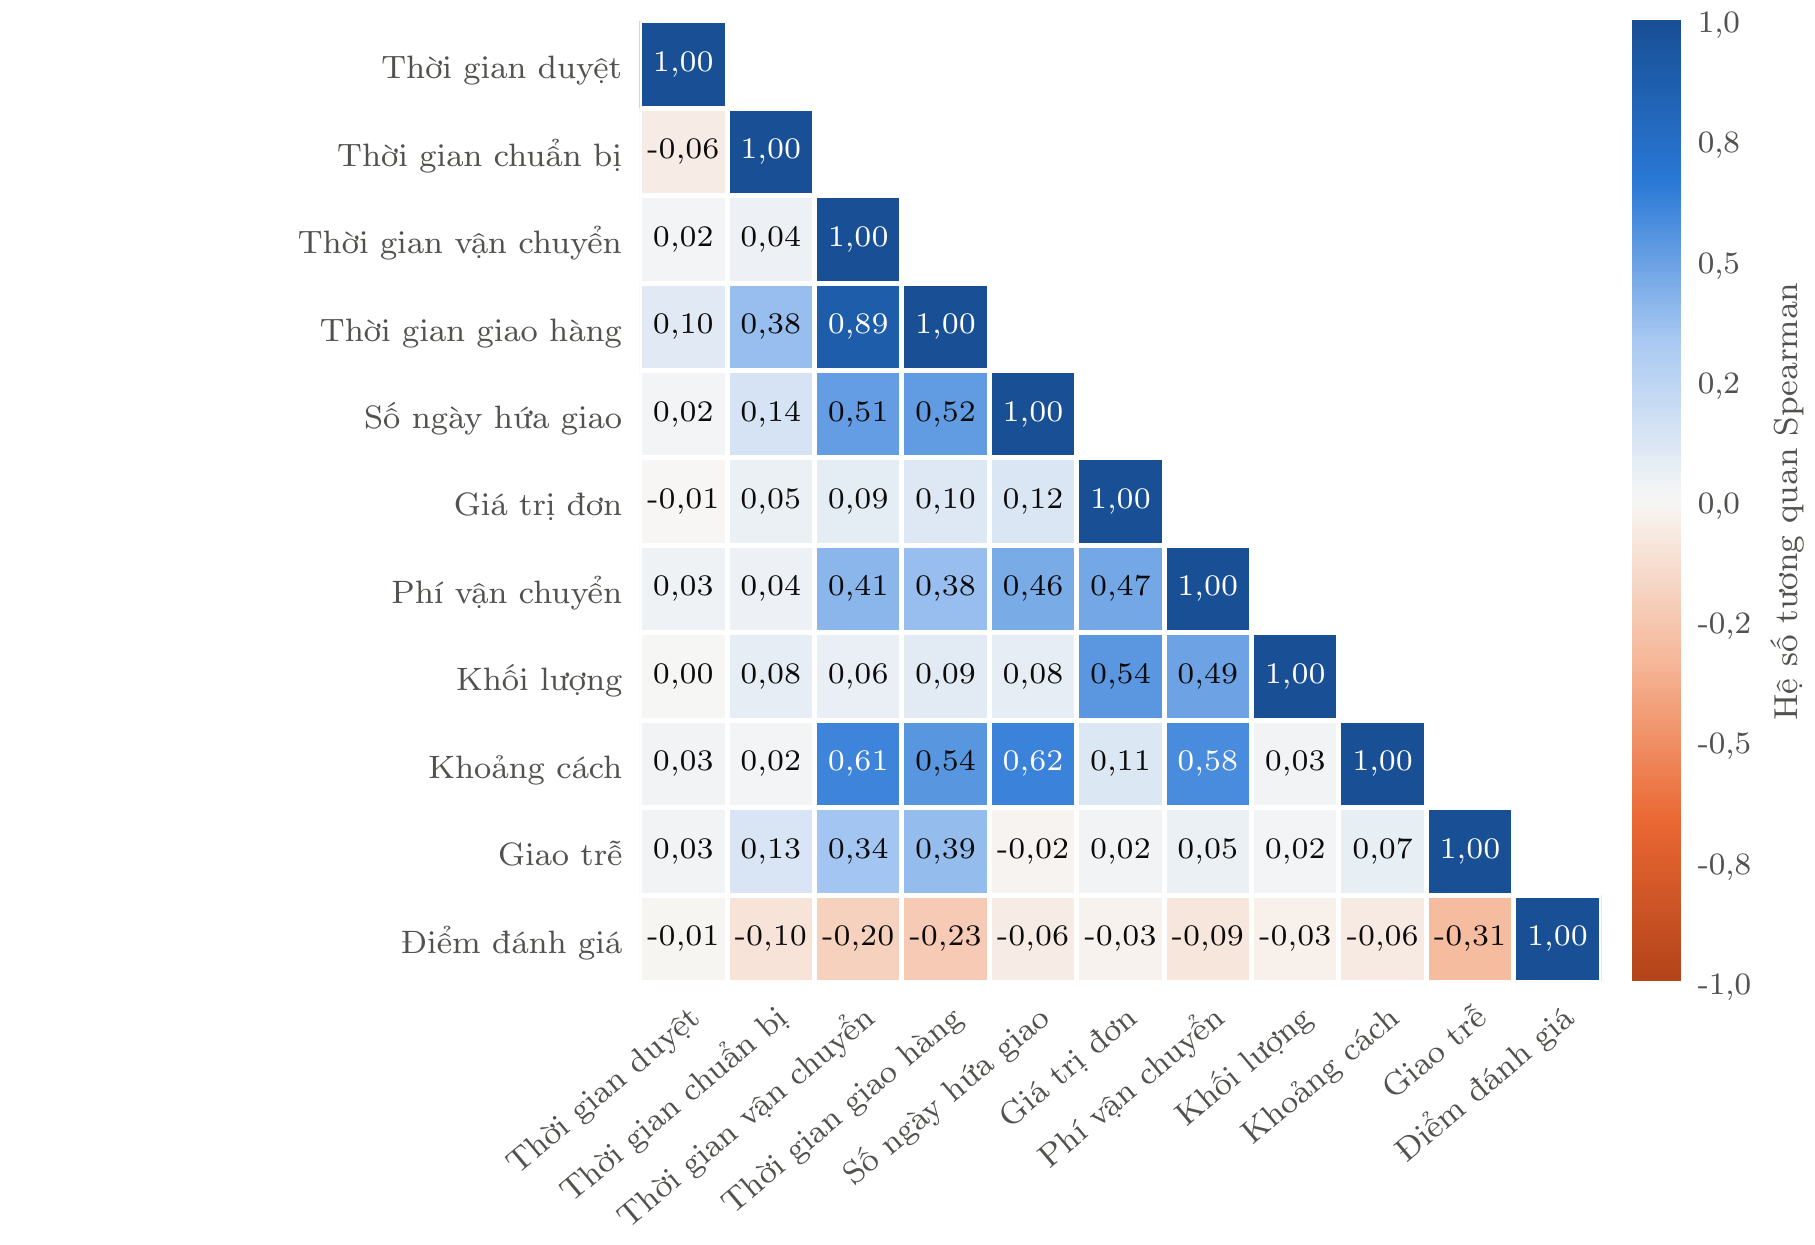
\includegraphics{Pictures/fig-eda-tuong-quan.png}
\caption{Ma trận tương quan Spearman giữa các thuộc tính ở mức đơn hàng (96.470 đơn đã giao)}
\label{fig:tuongquan}
\end{figure}

Ma trận cho thấy bốn điểm. Thứ nhất, điểm đánh giá tương quan mạnh nhất với cờ giao trễ ($-0{,}31$), mạnh hơn mọi thuộc tính về giá hay khối lượng; đây là dấu hiệu đầu tiên cho thấy giao trễ là vấn đề chính, và phần OLAP sẽ kiểm chứng điều này. Thứ hai, thời gian giao hàng gần như do thời gian vận chuyển quyết định (0,89), còn thời gian duyệt đơn hầu như không ảnh hưởng (0,10). Thứ ba, số ngày hứa giao (từ lúc mua đến ngày giao dự kiến) tương quan khá chặt với khoảng cách (0,62): đơn đi càng xa, sàn càng hứa giao lâu. Tuy vậy, số ngày hứa giao gần như không tương quan với giao trễ ($-0{,}02$), tức là hứa lâu không làm đơn ít bị trễ hơn, vì phần ngày cộng thêm chủ yếu chỉ bù cho quãng đường dài hơn. Điều quyết định một đơn có trễ hay không là \textit{khoảng dư}: số ngày hứa giao còn dư bao nhiêu so với thời gian giao thường lệ trên tuyến đó. Thứ tư, giá trị đơn, phí vận chuyển và khối lượng tăng giảm cùng nhau (tương quan 0,47-0,54), vì hàng nặng thường đắt hơn và tốn phí vận chuyển hơn. Nhưng cả ba gần như không liên quan đến giao trễ: đơn đắt hay rẻ, nặng hay nhẹ đều có khả năng trễ tương đương nhau, nên không thể dựa vào nhóm thuộc tính này để dự đoán giao trễ.

\subsubsection{Tỷ lệ giao trễ theo nhóm giá trị}

Hệ số tương quan chỉ đo quan hệ đơn điệu, nên ba thuộc tính được chia thành các khoảng và tính tỷ lệ trễ của từng khoảng (Hình~\ref{fig:trenhom}). Tỷ lệ trễ tăng đều theo khoảng cách, từ 4,6\% với đơn dưới 100 km lên 12,0\% với đơn trên 2.000 km. Với số ngày hứa giao, quan hệ có dạng hình chuông: đơn được hứa 21-25 ngày trễ nhiều nhất (8,1\%), còn đơn hứa trên 30 ngày ít trễ nhất (5,0\%), đúng với nhận xét về độ dư ở trên. Rõ nhất là thời gian người bán chuẩn bị hàng: đơn được bàn giao trong vòng một ngày chỉ trễ 3,9\%, còn đơn mất hơn 10 ngày trễ tới 29,4\% và bị chấm trung bình 3,32 điểm.

\begin{figure}[H]
\centering
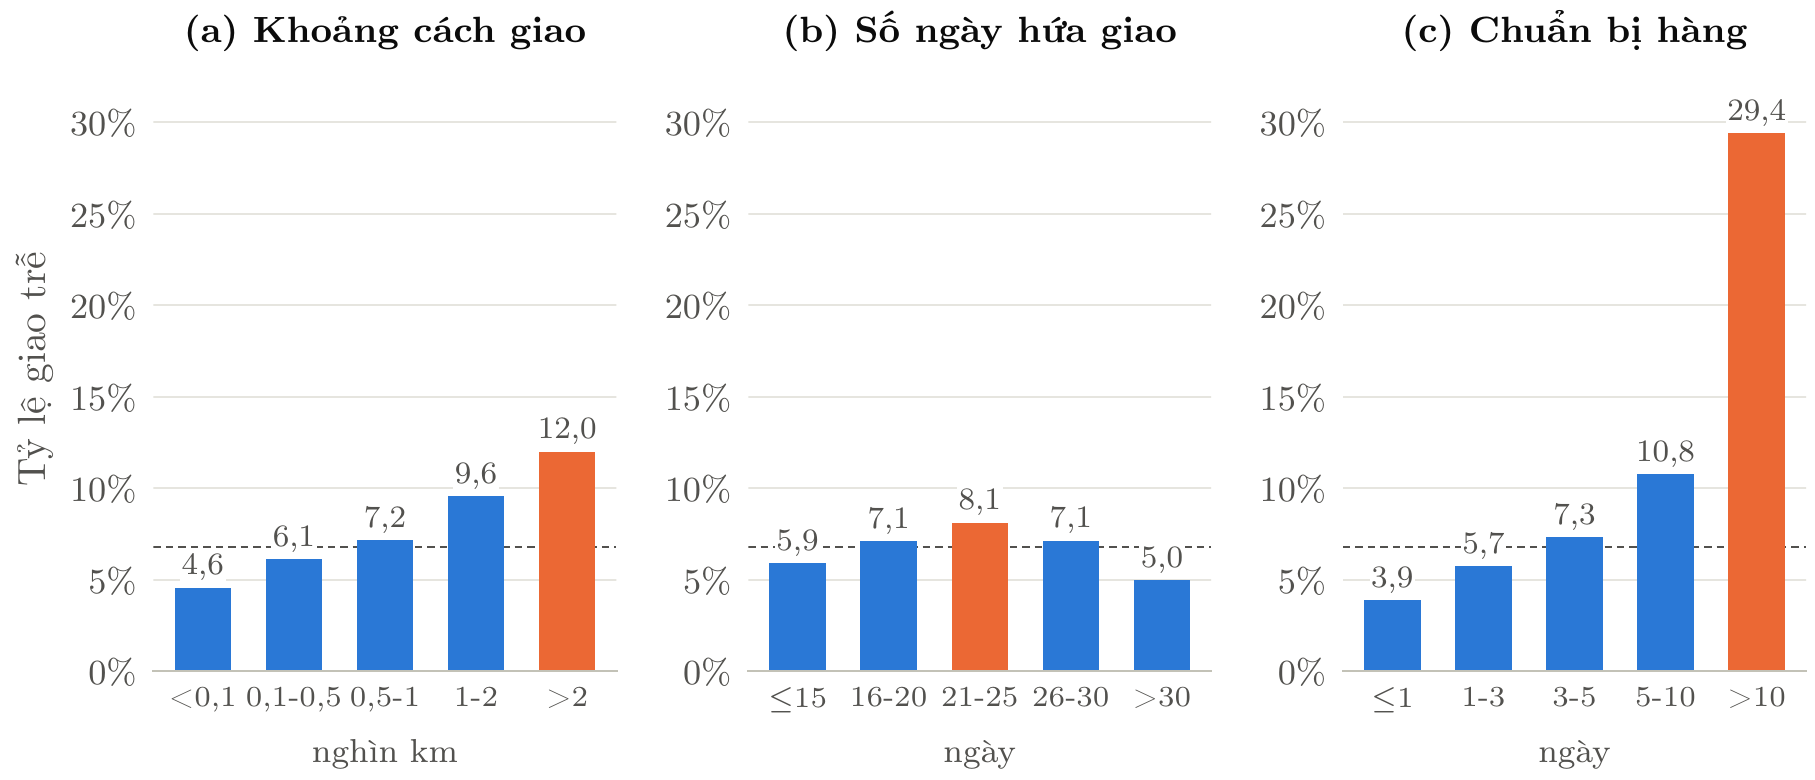
\includegraphics{Pictures/fig-eda-ty-le-tre-theo-nhom.png}
\caption{Tỷ lệ giao trễ theo khoảng cách giao (a), số ngày hứa giao (b) và thời gian người bán chuẩn bị hàng (c); đường đứt nét là tỷ lệ trễ chung 6,77\%}
\label{fig:trenhom}
\end{figure}

\subsubsection{Nhận xét}

Sau tiền xử lý, dữ liệu đã nhất quán: mỗi đơn có một trạng thái, một đánh giá, các mốc thời gian đúng thứ tự hoặc được để trống có lý do, và mọi khách hàng, người bán đều có thành phố, bang, vùng. Kết quả khám phá cũng định hướng cho các phần sau. Với kho dữ liệu, các thước đo về giao hàng và đánh giá phải tính ở mức đơn hàng, và cần chiều địa lý đủ chi tiết để phân tích theo tuyến giao. Với hệ hỗ trợ quyết định, thời gian chuẩn bị hàng, độ dư của ngày hứa giao và khoảng cách là những tín hiệu mạnh nhất về nguy cơ trễ; trong đó thời gian chuẩn bị hàng chỉ biết được khi người bán bàn giao cho đơn vị vận chuyển, nên đây là thời điểm hợp lý nhất để dự báo (mục~\ref{sec:dss}).

\clearpage
% !TeX root = ../main.tex
\section{Thiết kế kho dữ liệu theo mô hình đa chiều và quy trình ETL}\label{sec:thietke}
% !TeX root = ../../main.tex
\subsection{Thiết kế ý niệm}

\subsubsection{Mô hình kho dữ liệu}\label{sec:mohinhkho}

Có ba mô hình kho dữ liệu thường được nhắc tới: kho dữ liệu doanh nghiệp (Enterprise Data Warehouse -- EDW), Data Mart và kho dữ liệu ảo (Virtual Data Warehouse). Với phạm vi đã xác định ở mục~\ref{sec:phamvi}, đề tài xây dựng một \textit{Data Mart} lấy dữ liệu trực tiếp từ bộ dữ liệu nguồn.

EDW được thiết kế để gom dữ liệu của cả tổ chức, từ bán hàng đến nhân sự, kế toán, marketing, và thường phải tích hợp nhiều hệ thống nguồn khác nhau. Dữ liệu của đề tài thì chỉ có một mảng nghiệp vụ là đơn hàng và giao nhận, đến từ một nguồn duy nhất là 9 tập tin CSV của Olist (Bảng~\ref{tab:nguon}). Xây một EDW cho phạm vi này vừa thừa vừa không có dữ liệu để lấp đầy. Kho dữ liệu ảo cũng không phù hợp: mô hình này truy vấn thẳng trên dữ liệu nguồn mà không lưu bản đã xử lý, trong khi dữ liệu nguồn có hàng loạt vấn đề phải làm sạch trước (Bảng~\ref{tab:chatluong}) và truy vấn trên dữ liệu thô sẽ chậm hơn nhiều. Data Mart, ngược lại, tập trung vào một chủ đề và thường được tổ chức theo star schema hoặc snowflake schema, đúng với yêu cầu thiết kế đa chiều của đề tài.

Hệ thống phục vụ nhiều nhóm người dùng (ban điều hành, vận hành, quản lý người bán, chăm sóc khách hàng), nhưng tất cả đều khai thác cùng một mảng dữ liệu là \textit{đơn hàng}, nên một Data Mart vẫn đủ. Điểm yếu thường được nhắc tới của Data Mart là dễ trở thành một ``ốc đảo'' dữ liệu khi tổ chức có thêm nguồn khác. Để hạn chế điều này, các chiều thời gian, địa lý và sản phẩm được thiết kế theo dạng chiều đồng nhất (conformed dimensions), tức có cấu trúc và cách mã hóa đủ chung để Data Mart khác dùng lại được, chẳng hạn một Data Mart thanh toán trong tương lai.

\subsubsection{Hướng tiếp cận xây dựng mô hình}

Đi kèm với lựa chọn Data Mart, hệ thống được xây dựng theo hướng \textit{Bottom-up}: bắt đầu từ một Data Mart phục vụ một nhu cầu cụ thể, rồi mở rộng dần. Hướng này phù hợp với quy mô và thời gian của đề tài, vì Data Mart được thiết kế quanh đúng các chỉ số ở Bảng~\ref{tab:kpi} và các quyết định ở Bảng~\ref{tab:quyetdinh}, nên có thể đưa vào sử dụng ngay sau khi nạp dữ liệu, với chi phí và thời gian phát triển thấp.

Thứ tự triển khai là: xây Data Mart cho mảng bán hàng và giao nhận; xây quy trình ETL để làm sạch và nạp dữ liệu Olist vào Data Mart; xây các truy vấn OLAP, dashboard và thành phần DSS trên Data Mart. Khi có thêm nguồn dữ liệu, các Data Mart mới sẽ nối với Data Mart hiện tại qua các chiều đồng nhất nói trên. Đây cũng là cách khắc phục nhược điểm lớn nhất của Bottom-up, là các Data Mart xây riêng lẻ dễ rời rạc và khó tích hợp về sau.

\subsubsection{Kiến trúc tổng thể của hệ thống}\label{sec:kientruc}

Hệ thống theo kiến trúc ba tầng của kho dữ liệu, tách riêng phần lưu trữ, phần xử lý phân tích và phần trình bày để mỗi tầng phát triển độc lập. Hình~\ref{fig:kientruc} mô tả kiến trúc này.

% !TeX root = ../../main.tex
% Kiến trúc ba tầng của hệ thống
\begin{figure}[H]
\centering
\begin{tikzpicture}[
    tier/.style={rounded corners=4pt, fill=#1, draw=none, minimum width=15.2cm, anchor=south west, inner sep=0pt},
    tlabel/.style={font=\tiny\bfseries, text=white, rotate=90, anchor=center},
    box/.style={dwbox=#1, text width=3.3cm, minimum height=1.0cm},
    db/.style 2 args={dwdb=#1, text width=#2, font=\footnotesize},
    file/.style={draw=dwLine, fill=white, line width=0.4pt, font=\tiny\ttfamily, minimum width=1.4cm,
                 minimum height=0.5cm, inner sep=1pt}]
% tiers (bottom to top)
\node[tier=dwPaper, minimum height=1.65cm] (T0) at (0,0) {};
\node[tier=dwBlue!5, minimum height=4.35cm] (T1) at (0,1.9) {};
\node[tier=dwViolet!6, minimum height=2.0cm] (T2) at (0,6.5) {};
\node[tier=dwOrange!6, minimum height=2.1cm] (T3) at (0,8.75) {};
\foreach \T/\c/\l in {T0/dwMuted/NGUỒN, T1/dwBlue/TẦNG DƯỚI, T2/dwViolet/TẦNG GIỮA, T3/dwOrange/TẦNG TRÊN} {
  \fill[\c, rounded corners=4pt] (\T.south west) rectangle ([xshift=0.5cm]\T.north west);
  \fill[\c] ([xshift=0.25cm]\T.south west) rectangle ([xshift=0.5cm]\T.north west);
  \node[tlabel] at ([xshift=0.25cm]\T.west) {\l};
}
% sources
\foreach \n [count=\i] in {orders, order\_items, payments, reviews, customers, sellers, products, geolocation, translation}
  \node[file] at (1.45+\i*1.55-1.55, 0.55) {\n};
\node[font=\scriptsize, text=dwMuted, anchor=north east] at ([shift={(-5pt,-4pt)}]T0.north east) {9 tập tin CSV của Olist, 1.550.922 dòng};
% bottom tier
\node[dwbox=dwInkTwo, text width=5.2cm, minimum height=0.85cm] (etl) at (6.2,2.65)
  {\textbf{ETL} (Python + SQL)\\[-1pt]{\scriptsize Extract $\rightarrow$ Transformation $\rightarrow$ Load $\rightarrow$ Kiểm tra}};
\node[db={dwYellow}{2.6cm}] (stg) at (12.2,2.65) {\textbf{Staging}\\[-1pt]{\scriptsize\texttt{raw\_*}, \texttt{stg\_*}}};
\node[db={dwBlue}{3.3cm}] (dm) at (6.2,4.75) {\textbf{Data Mart}\\[-1pt]{\scriptsize snowflake schema \texttt{dm}}\\[-1pt]{\scriptsize\texttt{fact\_sales} + 7 bảng chiều}};
\node[db={dwAqua}{2.8cm}] (meta) at (2.55,4.75) {\textbf{Metadata}\\[-1pt]{\scriptsize từ điển, nguồn gốc dữ liệu,}\\[-1pt]{\scriptsize nhật ký ETL, đối soát}};
\node[db={dwOrange}{2.6cm}] (dss) at (12.2,4.75) {\textbf{Kết quả DSS}\\[-1pt]{\scriptsize schema \texttt{dss}}};
% middle tier
\node[box=dwViolet, text width=7.4cm] (olap) at (7.4,7.5)
  {\textbf{ROLAP trên PostgreSQL}\\[-1pt]{\scriptsize roll-up, drill-down, slice, dice, pivot bằng \texttt{GROUP BY}, \texttt{ROLLUP}, \texttt{CUBE}}};
% top tier
\node[box=dwOrange] (rep) at (2.7,9.8) {\textbf{Truy vấn, báo cáo}\\[-1pt]{\scriptsize thư viện truy vấn OLAP}};
\node[box=dwOrange] (dash) at (7.4,9.8) {\textbf{Dashboard}\\[-1pt]{\scriptsize doanh thu, giao hàng, đánh giá}};
\node[box=dwOrange] (dssui) at (12.2,9.8) {\textbf{Hệ hỗ trợ quyết định}\\[-1pt]{\scriptsize cảnh báo giao trễ}};
% flows
\draw[dwarrow] (6.2,1.65) -- (etl.south);
\draw[dwarrow, {Stealth[length=2mm,width=1.5mm]}-{Stealth[length=2mm,width=1.5mm]}] (etl.east) -- (stg.west);
\draw[dwarrow] (etl.north) -- (dm.south);
\draw[dwdash, rounded corners=3pt] (etl.west) -| (meta.south);
\draw[dwarrow] (dm.north) -- (dm.north |- olap.south);
\draw[dwarrow, rounded corners=3pt] (olap.west) -| (rep.south);
\draw[dwarrow] (olap.north) -- (dash.south);
\draw[dwarrow] (dm.east) -- node[dwlabel, above] {đặc trưng} (dss.west);
\draw[dwarrow, {Stealth[length=2mm,width=1.5mm]}-{Stealth[length=2mm,width=1.5mm]}] (dss.north) -- (dssui.south);
\end{tikzpicture}
\caption{Sơ đồ kiến trúc ba tầng của hệ thống}
\label{fig:kientruc}
\end{figure}


Dữ liệu nguồn là 9 tập tin CSV của Olist. Quy trình ETL viết bằng Python đọc các tập tin này, nạp nguyên trạng vào khu vực staging rồi làm sạch, biến đổi và nạp vào Data Mart. Khu vực staging là một schema riêng trong PostgreSQL, chứa cả dữ liệu thô lẫn dữ liệu đã làm sạch, và là nơi xử lý toàn bộ các vấn đề ở Bảng~\ref{tab:chatluong}.

Tầng dưới (Bottom tier) là Data Mart bán hàng và giao nhận, tổ chức theo snowflake schema trên PostgreSQL. Bên cạnh Data Mart có kho metadata (metadata repository) lưu từ điển dữ liệu và nguồn gốc dữ liệu, cùng hai chức năng: giám sát (Monitoring) qua nhật ký chạy ETL, và quản trị (Administrator) qua việc chỉ cấp quyền đọc cho người dùng phân tích.

Tầng giữa (Middle tier) là OLAP server theo mô hình ROLAP. Khối dữ liệu đa chiều được biểu diễn trực tiếp bằng các bảng của Data Mart, và các phép \texttt{slice}, \texttt{dice}, \texttt{drill-down}, \texttt{roll-up}, \texttt{pivot} được viết thành truy vấn SQL. ROLAP được chọn vì dữ liệu đã nằm sẵn trong cơ sở dữ liệu quan hệ và quy mô hiện tại cho phép tổng hợp trực tiếp mà vẫn đủ nhanh; nếu dùng MOLAP thì phải thêm một máy chủ khối riêng và một bước xử lý khối mỗi lần nạp dữ liệu.

Tầng trên (Top tier) gồm công cụ truy vấn và báo cáo, dashboard theo dõi doanh thu, giao hàng, đánh giá và người bán, cùng thành phần hệ hỗ trợ quyết định khai thác dữ liệu từ kho.

Toàn bộ phần lưu trữ (staging, Data Mart, metadata) dùng chung một hệ quản trị cơ sở dữ liệu là PostgreSQL. 
% !TeX root = ../../main.tex
\subsection{Mô hình dữ liệu đa chiều}

Mô hình đa chiều được thiết kế theo bốn bước: chọn quy trình nghiệp vụ, xác định granularity, xác định các chiều và xác định các thước đo \cite{kimball}. Mỗi bước dưới đây đều dựa trên kết quả phân tích ở phần trước.

\subsubsection{Xác định quy trình nghiệp vụ}

Quy trình nghiệp vụ là một hoạt động thực tế của doanh nghiệp tạo ra các sự kiện đo lường được. Nhìn vào vòng đời đơn hàng (Bảng~\ref{tab:quytrinh}) và danh sách chỉ số (Bảng~\ref{tab:kpi}), nhóm xác định ba quy trình cần mô hình hóa. \textit{Bán hàng} là quy trình trung tâm: mỗi sản phẩm được bán trong đơn cùng giá, phí vận chuyển và người bán; mọi chỉ số doanh thu và hiệu quả người bán đều tính từ đây. \textit{Giao hàng} ghi lại các mốc từ lúc mua, duyệt, bàn giao vận chuyển đến lúc khách nhận hàng, so với ngày dự kiến, và là nguồn của các chỉ số thời gian giao và tỷ lệ trễ. \textit{Đánh giá} ghi lại điểm khách hàng chấm sau khi nhận hàng.

Quy trình thanh toán không được đưa vào. Một đơn có thể có nhiều khoản thanh toán, và quy trình này chỉ phục vụ một chỉ số phụ về cơ cấu phương thức thanh toán đã nằm ngoài phạm vi (mục~\ref{sec:phamvi}).

Ba quy trình còn lại thực chất là các giai đoạn nối tiếp nhau của cùng một đơn hàng. Vì vậy nhóm gộp chúng vào một bảng fact duy nhất dạng \textit{accumulating snapshot} \cite{kimball}: mỗi dòng là một đối tượng đi qua cả quy trình, mỗi mốc được lưu bằng một cột ngày riêng, và thước đo gồm cả giá trị phát sinh lẫn khoảng thời gian giữa các mốc. Với một bảng fact, doanh thu, giao hàng và đánh giá có thể phân tích cùng lúc mà không phải ghép nhiều bảng fact với nhau.

\subsubsection{Xác định granularity}\label{sec:granularity}

Granularity, tức mức chi tiết của mỗi dòng dữ liệu, là quyết định ảnh hưởng lớn nhất đến dung lượng kho và những câu hỏi mà kho trả lời được \cite{inmon}. Granularity của bảng fact được chọn như sau:

\begin{center}
\textit{Mỗi dòng của bảng fact là một sản phẩm trong một đơn hàng}, xác định bởi cặp khóa (\code{order\_id}, \code{order\_item\_id}).
\end{center}

Đây là mức chi tiết thấp nhất của dữ liệu nguồn, vì giá bán, phí vận chuyển, sản phẩm và người bán đều được ghi theo từng dòng sản phẩm. Nếu chọn mức đơn hàng, kho sẽ mất thông tin sản phẩm và người bán ở các đơn nhiều sản phẩm hoặc nhiều người bán. Từ mức dòng sản phẩm vẫn tổng hợp lên được mức đơn hàng, người bán, ngành hàng và khu vực, nên mọi chỉ số ở Bảng~\ref{tab:kpi} đều tính được. Về dung lượng, bảng fact có 112.650 dòng ứng với 98.666 đơn có sản phẩm; với khoảng 20 cột, nhóm ước tính bảng chiếm 15-20 MB chưa kể chỉ mục (thực tế sau khi nạp là 17 MB), nên không cần tổng hợp trước để tiết kiệm chỗ.

Cái giá của lựa chọn này là thông tin giao hàng và đánh giá, vốn ghi theo đơn, bị lặp lại trên mọi dòng sản phẩm của cùng một đơn. Nếu lấy trung bình trực tiếp trên bảng fact, đơn nhiều sản phẩm sẽ được tính nhiều lần. Nhóm xử lý bằng cách tổng hợp các thước đo này trên tập đơn hàng phân biệt, sẽ trình bày ở mục~\ref{sec:dodo}.

Có 775 đơn hàng không có dòng sản phẩm nào, phần lớn ở trạng thái \code{unavailable} (603 đơn) và \code{canceled} (164 đơn). Các đơn này không xuất hiện trong bảng fact nên không được tính vào chỉ số của kho.

\subsubsection{Xác định các chiều và phân cấp}

Các chiều được rút ra từ cách người dùng muốn xem các chỉ số: theo thời gian, theo sản phẩm và ngành hàng, theo khách hàng, theo người bán và theo khu vực (Bảng~\ref{tab:quyetdinh}). Bảng~\ref{tab:chieu} liệt kê các chiều, phân cấp (hierarchies) và số dòng ước tính của từng chiều; Hình~\ref{fig:phancap} vẽ lại các phân cấp này.

\begin{table}[H]
\centering
\small\setstretch{1.1}
\caption{Các chiều phân tích và phân cấp}
\label{tab:chieu}
\begin{tabularx}{\linewidth}{|P{2.2cm}|>{\raggedright\arraybackslash}X|P{4.3cm}|P{2.4cm}|}
\hline
\textbf{Chiều} & \textbf{Thuộc tính chính} & \textbf{Phân cấp} & \textbf{Số dòng ước tính}\\ \hline
Thời gian & Ngày, tháng, quý, năm, thứ trong tuần & Ngày $\rightarrow$ Tháng $\rightarrow$ Quý $\rightarrow$ Năm & 1.096 (các năm 2016-2018)\\ \hline
Sản phẩm & Mã sản phẩm, khối lượng, kích thước, số ảnh & Sản phẩm $\rightarrow$ Ngành hàng & 32.951\\ \hline
Ngành hàng & Tên ngành hàng tiếng Bồ Đào Nha và tiếng Anh & -- & 74\\ \hline
Khách hàng & Mã khách hàng (\code{customer\_unique\_id}), mã bưu chính & Khách hàng $\rightarrow$ Thành phố $\rightarrow$ Bang $\rightarrow$ Vùng & 96.096\\ \hline
Người bán & Mã người bán, mã bưu chính & Người bán $\rightarrow$ Thành phố $\rightarrow$ Bang $\rightarrow$ Vùng & 3.095\\ \hline
Thành phố & Tên thành phố, vĩ độ, kinh độ & Thành phố $\rightarrow$ Bang & 4.341\\ \hline
Bang & Mã bang, tên bang, vùng & Bang $\rightarrow$ Vùng & 27\\ \hline
\end{tabularx}
\end{table}

Ngoài số dòng ở Bảng~\ref{tab:chieu}, mỗi bảng chiều có thêm một dòng không xác định (khóa $-1$) để các bản ghi thiếu thông tin, như đơn chưa có ngày nhận hàng, vẫn nối được vào bảng chiều. Riêng chiều ngành hàng, con số 74 đã gồm ngành ``không xác định'' dành cho 610 sản phẩm thiếu ngành.

% !TeX root = ../../main.tex
% Phân cấp của các chiều phân tích
\begin{figure}[H]
\centering
\resizebox{\linewidth}{!}{%
\begin{tikzpicture}[node distance=0.42cm,
    head/.style={dwhead=#1, text width=2.5cm, inner sep=3pt, rounded corners=2pt},
    lv/.style={dwbox=#1, text width=2.5cm, inner sep=3.5pt, font=\footnotesize},
    up/.style={-{Stealth[length=1.8mm]}, line width=0.6pt, draw=dwInkTwo}]
\node[head=dwBlue] (t0) at (0,0) {Thời gian};
\node[lv=dwBlue, below=of t0] (t1) {Ngày};
\node[lv=dwBlue, below=of t1] (t2) {Tháng};
\node[lv=dwBlue, below=of t2] (t3) {Quý};
\node[lv=dwBlue, below=of t3] (t4) {Năm};
\node[head=dwAqua] (p0) at (3.6,0) {Sản phẩm};
\node[lv=dwAqua, below=of p0] (p1) {Sản phẩm};
\node[lv=dwAqua, below=of p1] (p2) {Ngành hàng};
\node[head=dwOrange] (c0) at (7.2,0) {Khách hàng};
\node[lv=dwOrange, below=of c0] (c1) {Khách hàng};
\node[lv=dwYellow, below=of c1] (c2) {Thành phố};
\node[lv=dwYellow, below=of c2] (c3) {Bang};
\node[lv=dwYellow, below=of c3] (c4) {Vùng};
\node[head=dwViolet] (s0) at (10.8,0) {Người bán};
\node[lv=dwViolet, below=of s0] (s1) {Người bán};
\foreach \a/\b in {t1/t2, t2/t3, t3/t4, p1/p2, c1/c2, c2/c3, c3/c4} \draw[up] (\a) -- (\b);
\draw[up, rounded corners=3pt] (s1.south) |- (c2.east);
\node[font=\scriptsize, text=dwInkTwo, align=left, anchor=north west] at ([xshift=0.1cm, yshift=-0.2cm]s1.south)
  {phần địa lý\\(Thành phố $\rightarrow$ Bang $\rightarrow$ Vùng)\\dùng chung với khách hàng};
\begin{scope}[on background layer]
  \node[fill=dwYellow!8, rounded corners=4pt, fit=(c2)(c4), inner sep=5pt] {};
\end{scope}
\end{tikzpicture}}
\caption{Phân cấp của các chiều phân tích trong Data Mart; mũi tên chỉ hướng roll-up (từ chi tiết lên tổng hợp), drill-down đi theo chiều ngược lại}
\label{fig:phancap}
\end{figure}


Chiều thời gian được dùng theo nhiều vai trò. Bảng fact có sáu cột ngày (mua, duyệt, bàn giao vận chuyển, nhận hàng, giao dự kiến và đánh giá), cả sáu cùng trỏ về một chiều thời gian duy nhất, mỗi cột là một vai trò khác nhau (role-playing dimension) \cite{kimball}. Chiều này được sinh đủ cho các năm 2016-2018 để bao trọn mọi mốc thời gian trong dữ liệu, từ 04/9/2016 đến 12/11/2018.

Khách hàng và người bán cùng trỏ về chiều thành phố và chiều bang. Nhờ dùng chung, có thể phân tích tuyến giao hàng từ bang của người bán đến bang của khách hàng mà không lo hai bên mã hóa địa lý khác nhau. Đây cũng là các chiều đồng nhất đã nhắc tới ở mục~\ref{sec:mohinhkho}. Dữ liệu nguồn không có thông tin vùng, nên nhóm tự gán 27 bang vào năm vùng địa lý của Brazil (Norte, Nordeste, Centro-Oeste, Sudeste, Sul) ở bước transformation.

Chiều sản phẩm được tách thành bảng ngành hàng, còn chiều khách hàng và người bán được tách thành bảng thành phố và bảng bang, theo dạng snowflake. Cách tách này tránh lặp lại tên ngành hàng và thông tin địa lý trên hàng chục nghìn dòng, và làm các phân cấp hiện rõ ra thành bảng, thuận tiện cho \texttt{roll-up} và \texttt{drill-down}. Riêng mã đơn hàng (\code{order\_id}) không có thuộc tính mô tả nào nên được giữ thẳng trong bảng fact dưới dạng degenerate dimension \cite{kimball}, dùng để gom các dòng sản phẩm của cùng một đơn.

\subsubsection{Xác định các thước đo}\label{sec:dodo}

Thước đo được rút ra từ các chỉ số ở Bảng~\ref{tab:kpi} và được phân loại theo khả năng cộng dồn. Thước đo cộng được (additive) cộng được theo mọi chiều; thước đo cộng được một phần (semi-additive) chỉ cộng được theo một số chiều; thước đo không cộng được (non-additive) phải tổng hợp bằng hàm khác như trung bình hay tỷ lệ \cite{kimball}. Bảng~\ref{tab:dodo} liệt kê các thước đo được lưu trong bảng fact.

\begingroup\small\setstretch{1.1}
\begin{longtable}{|P{3.2cm}|P{4.4cm}|P{2.4cm}|P{3.6cm}|}
\caption{Các thước đo trong bảng fact}\label{tab:dodo}\\
\hline
\textbf{Thước đo} & \textbf{Cách tính} & \textbf{Loại} & \textbf{Hàm tổng hợp}\\ \hline \endfirsthead
\hline
\textbf{Thước đo} & \textbf{Cách tính} & \textbf{Loại} & \textbf{Hàm tổng hợp}\\ \hline \endhead
Giá bán (\code{price}) & Giá của dòng sản phẩm & Cộng được & Tổng\\ \hline
Phí vận chuyển (\code{freight\_value}) & Phí vận chuyển của dòng sản phẩm & Cộng được & Tổng\\ \hline
Thời gian duyệt đơn & Thời điểm duyệt $-$ Thời điểm mua (ngày) & Không cộng được, theo đơn & Trung bình trên đơn hàng phân biệt\\ \hline
Thời gian chuẩn bị hàng & Thời điểm bàn giao vận chuyển $-$ Thời điểm duyệt (ngày) & Không cộng được, theo đơn & Trung bình trên đơn hàng phân biệt\\ \hline
Thời gian vận chuyển & Thời điểm nhận hàng $-$ Thời điểm bàn giao vận chuyển (ngày) & Không cộng được, theo đơn & Trung bình trên đơn hàng phân biệt\\ \hline
Thời gian giao hàng & Thời điểm nhận hàng $-$ Thời điểm mua (ngày) & Không cộng được, theo đơn & Trung bình trên đơn hàng phân biệt\\ \hline
Cờ giao trễ & Bằng 1 nếu ngày nhận hàng sau ngày giao dự kiến, ngược lại bằng 0 & Không cộng được, theo đơn & Tỷ lệ trên đơn hàng phân biệt\\ \hline
Điểm đánh giá & Điểm từ 1 đến 5 sao của đơn hàng & Không cộng được, theo đơn & Trung bình trên đơn hàng phân biệt\\ \hline
\end{longtable}
\endgroup

Giá bán và phí vận chuyển được ghi đúng ở granularity của bảng fact nên cộng trực tiếp theo mọi chiều. Các khoảng thời gian, cờ giao trễ và điểm đánh giá thì có cùng giá trị trên mọi dòng của một đơn; khi tổng hợp, chỉ lấy một giá trị cho mỗi đơn (gom theo \code{order\_id}) rồi mới tính trung bình hay tỷ lệ. Những chỉ số như số đơn hàng, giá trị đơn trung bình hay tỷ lệ phí vận chuyển không được lưu sẵn mà tính lúc truy vấn, vì giá trị của chúng phụ thuộc vào mức tổng hợp.

Nguồn chỉ có một điểm đánh giá cho mỗi đơn, nên ở 1.278 đơn có nhiều người bán, mọi người bán trong đơn dùng chung một điểm. Đây là giới hạn của dữ liệu cần nhớ khi đánh giá mức độ hài lòng theo từng người bán.

\subsubsection{Data Cube và các phép toán OLAP}\label{sec:datacube}

Data Cube là cách nhìn dữ liệu đa chiều: mỗi trục là một góc nhìn phân tích, mỗi ô chứa giá trị tổng hợp của thước đo tại giao điểm của các chiều \cite{han}. Với thiết kế ở trên, khối dữ liệu của hệ thống có các chiều chính là thời gian, ngành hàng và khu vực của khách hàng và người bán; thước đo là doanh thu, phí vận chuyển, thời gian giao hàng, tỷ lệ trễ và điểm đánh giá. Hình~\ref{fig:datacube} minh họa một khối ba chiều: ô được tô màu là doanh thu của ngành \code{watches\_gifts} tại bang SP trong quý 3/2017.

% !TeX root = ../../main.tex
% Minh họa khối dữ liệu ba chiều: thời gian x ngành hàng x khu vực
\begin{figure}[H]
\centering
\begin{tikzpicture}[x={(1cm,0cm)}, y={(0cm,1cm)}, z={(0.55cm,0.36cm)}, font=\footnotesize, line join=round]
\foreach \i in {0,...,3} \foreach \j in {0,...,2}
  \draw[white, line width=0.8pt, fill=dwBlue!10] (\i,\j,0) -- ++(1,0,0) -- ++(0,1,0) -- ++(-1,0,0) -- cycle;
\foreach \i in {0,...,3} \foreach \k in {0,...,2}
  \draw[white, line width=0.8pt, fill=dwBlue!22] (\i,3,\k) -- ++(1,0,0) -- ++(0,0,1) -- ++(-1,0,0) -- cycle;
\foreach \j in {0,...,2} \foreach \k in {0,...,2}
  \draw[white, line width=0.8pt, fill=dwBlue!35] (4,\j,\k) -- ++(0,0,1) -- ++(0,1,0) -- ++(0,0,-1) -- cycle;
\draw[dwBlue!60!black, line width=0.5pt] (0,0,0) -- (4,0,0) -- (4,3,0) -- (0,3,0) -- cycle;
\draw[dwBlue!60!black, line width=0.5pt] (0,3,0) -- (0,3,3) -- (4,3,3) -- (4,0,3) -- (4,0,0);
\draw[dwBlue!60!black, line width=0.5pt] (4,3,0) -- (4,3,3);
\draw[white, line width=0.8pt, fill=dwOrange] (2,1,0) -- ++(1,0,0) -- ++(0,1,0) -- ++(-1,0,0) -- cycle;
\node[font=\scriptsize\bfseries, text=white] at (2.5,1.5,0) {38,7};
\foreach \i/\t in {0/Q1, 1/Q2, 2/Q3, 3/Q4} \node[below, text=dwInkTwo] at (\i+0.5,0,0) {\t};
\node[below=0.42cm, text=dwInk] at (2,0,0) {\textbf{Thời gian} (quý, năm 2017)};
\foreach \j/\t in {0/health\_beauty, 1/watches\_gifts, 2/bed\_bath\_table}
  \node[left, font=\scriptsize\ttfamily, text=dwInkTwo] at (0,\j+0.5,0) {\t};
\node[rotate=90, text=dwInk] at (-2.95,1.5,0) {\textbf{Ngành hàng}};
\foreach \k/\t in {0/SP, 1/RJ, 2/MG} \node[right, font=\scriptsize, text=dwInkTwo] at (4,0,\k+0.5) {\t};
\node[right, text=dwInk] at (4.6,0.2,3.5) {\textbf{Khu vực} (bang)};
\draw[dwOrange, line width=0.6pt, -{Stealth[length=2mm]}] (3.05,1.5,0) -- (6.0,-0.15,0);
\node[right, align=left, font=\scriptsize, text=dwInkTwo] at (6.05,-0.15,0)
  {\textbf{Một ô của khối:} doanh thu (nghìn BRL)\\của \texttt{watches\_gifts} tại SP trong quý 3/2017,\\
   tức \texttt{SUM(price)} của các dòng fact\\thỏa đồng thời cả ba điều kiện};
\end{tikzpicture}
\caption{Minh họa khối dữ liệu với ba chiều thời gian, ngành hàng và khu vực; thước đo trong mỗi ô là doanh thu}
\label{fig:datacube}
\end{figure}


Như đã nói ở mục~\ref{sec:kientruc}, khối dữ liệu được hiện thực theo ROLAP, các phép toán OLAP là truy vấn SQL trên các bảng của Data Mart. Bảng~\ref{tab:olap} cho ví dụ về cách mỗi phép toán phục vụ một nhu cầu phân tích; kết quả chạy thật của các phép toán này được trình bày ở mục~\ref{sec:olap}.

\begin{table}[H]
\centering
\small\setstretch{1.1}
\caption{Ví dụ áp dụng các phép toán OLAP}
\label{tab:olap}
\begin{tabularx}{\linewidth}{|P{2.2cm}|>{\raggedright\arraybackslash}X|P{4.6cm}|}
\hline
\textbf{Phép toán} & \textbf{Ví dụ áp dụng} & \textbf{Nhu cầu phân tích}\\ \hline
Roll-up & Tổng hợp doanh thu từ theo ngày lên theo tháng, quý, năm; tổng hợp từ thành phố lên bang và vùng. & Theo dõi xu hướng doanh thu theo thời gian và khu vực.\\ \hline
Drill-down & Từ tỷ lệ giao trễ của một vùng, đi xuống từng bang rồi từng thành phố. & Xác định khu vực có tỷ lệ giao trễ cao.\\ \hline
Slice & Chọn một giá trị trên chiều thời gian, ví dụ chỉ xem dữ liệu năm 2018. & So sánh kết quả kinh doanh trong một kỳ.\\ \hline
Dice & Chọn đồng thời giá trị trên nhiều chiều, ví dụ một số ngành hàng tại các bang SP, RJ, MG trong quý 4/2017. & Phân tích sâu một nhóm ngành hàng tại các thị trường chính.\\ \hline
Pivot & Hoán đổi trục ngành hàng và trục khu vực trong bảng điểm đánh giá trung bình. & So sánh mức độ hài lòng theo nhiều góc nhìn.\\ \hline
\end{tabularx}
\end{table}

% !TeX root = ../../main.tex
\subsection{Thiết kế mức logic}

\subsubsection{Lựa chọn lược đồ}\label{sec:luocdo}

Mô hình đa chiều có thể được tổ chức theo ba dạng lược đồ: star schema, snowflake schema và fact constellation \cite{han}. Vì ba quy trình nghiệp vụ đã được gộp vào một bảng fact duy nhất, fact constellation (dành cho trường hợp nhiều bảng fact dùng chung bảng chiều) không còn cần thiết. Lựa chọn còn lại là giữa star schema và snowflake schema; nhóm dùng \textit{snowflake schema}.

Lý do chính nằm ở dữ liệu địa lý. Cả khách hàng lẫn người bán đều có thành phố và bang; nếu dùng star schema, hai bảng chiều khách hàng và người bán sẽ mỗi bảng giữ một bản sao thông tin địa lý, và chỉ cần một bên chuẩn hóa tên thành phố khác bên kia là phân tích tuyến giao hàng sẽ sai. Tách thành phố và bang ra bảng riêng dùng chung giúp hai bên luôn khớp nhau. Thêm vào đó, các phân cấp Sản phẩm $\rightarrow$ Ngành hàng và Thành phố $\rightarrow$ Bang $\rightarrow$ Vùng hiện ra thành các bảng riêng, nên câu lệnh \texttt{roll-up} hay \texttt{drill-down} chỉ cần nối thêm một bảng.

Đổi lại, truy vấn trên snowflake schema cần nhiều phép kết nối hơn star schema. Với khoảng 112.650 dòng trong bảng fact, chi phí này chấp nhận được, và kết quả đo ở mục~\ref{sec:olap} xác nhận điều đó. Riêng chiều thời gian vẫn để dạng phẳng, không tách thành các bảng tháng, quý, năm, vì đây là chiều dùng nhiều nhất và chỉ có hơn một nghìn dòng.

\subsubsection{Thiết kế bảng fact}

Bảng fact của Data Mart tên là \code{fact\_sales}, có granularity là một sản phẩm trong một đơn hàng (mục~\ref{sec:granularity}) và khóa chính là cặp (\code{order\_id}, \code{order\_item\_id}). Cấu trúc bảng được mô tả trong Bảng~\ref{tab:fact}.

\begingroup\small\setstretch{1.1}
\begin{longtable}{|P{3.9cm}|P{1.7cm}|P{4.2cm}|P{3.9cm}|}
\caption{Cấu trúc bảng fact \code{fact\_sales}}\label{tab:fact}\\
\hline
\textbf{Cột} & \textbf{Kiểu} & \textbf{Ý nghĩa} & \textbf{Nguồn}\\ \hline \endfirsthead
\hline
\textbf{Cột} & \textbf{Kiểu} & \textbf{Ý nghĩa} & \textbf{Nguồn}\\ \hline \endhead
\code{order\_id} & varchar & Mã đơn hàng (degenerate dimension), một phần của khóa chính & \code{order\_items}\\ \hline
\code{order\_item\_id} & int & Số thứ tự sản phẩm trong đơn, một phần của khóa chính & \code{order\_items}\\ \hline
\code{product\_key} & int & Khóa ngoại đến \code{dim\_product} & Tra cứu theo \code{product\_id}\\ \hline
\code{seller\_key} & int & Khóa ngoại đến \code{dim\_seller} & Tra cứu theo \code{seller\_id}\\ \hline
\code{customer\_key} & int & Khóa ngoại đến \code{dim\_customer} & Tra cứu theo \code{customer\_unique\_id}\\ \hline
\code{purchase\_date\_key} & int & Ngày mua & \code{orders}\\ \hline
\code{approved\_date\_key} & int & Ngày duyệt đơn & \code{orders}\\ \hline
\code{carrier\_date\_key} & int & Ngày bàn giao vận chuyển & \code{orders}\\ \hline
\code{delivered\_date\_key} & int & Ngày khách nhận hàng & \code{orders}\\ \hline
\code{estimated\_date\_key} & int & Ngày giao dự kiến & \code{orders}\\ \hline
\code{review\_date\_key} & int & Ngày tạo đánh giá & \code{order\_reviews}\\ \hline
\code{order\_status} & varchar & Trạng thái đơn hàng & \code{orders}\\ \hline
\code{price} & decimal & Giá bán của dòng sản phẩm & \code{order\_items}\\ \hline
\code{freight\_value} & decimal & Phí vận chuyển của dòng sản phẩm & \code{order\_items}\\ \hline
\code{approval\_days} & decimal & Thời gian duyệt đơn (ngày) & Tính từ \code{orders}\\ \hline
\code{handling\_days} & decimal & Thời gian chuẩn bị hàng (ngày) & Tính từ \code{orders}\\ \hline
\code{shipping\_days} & decimal & Thời gian vận chuyển (ngày) & Tính từ \code{orders}\\ \hline
\code{delivery\_days} & decimal & Tổng thời gian giao hàng (ngày) & Tính từ \code{orders}\\ \hline
\code{is\_late} & smallint & Cờ giao trễ (1: trễ, 0: đúng hạn) & Tính từ \code{orders}\\ \hline
\code{review\_score} & smallint & Điểm đánh giá của đơn hàng (1-5) & \code{order\_reviews}\\ \hline
\end{longtable}
\endgroup

Có thể chia các cột thành ba nhóm. Nhóm đầu là khóa: mã đơn hàng và số thứ tự sản phẩm tạo thành khóa chính, còn các khóa ngoại trỏ đến bảng chiều bằng surrogate key chứ không bằng mã gốc của nguồn. Nhóm thứ hai là sáu cột ngày, cùng trỏ đến \code{dim\_date}, mỗi cột ứng với một mốc trong vòng đời đơn hàng (Hình~\ref{fig:vongdoi}). Mốc chưa xảy ra, chẳng hạn ngày nhận hàng của đơn đang giao, được trỏ đến một khóa đặc biệt mang nghĩa ``không xác định''. Nhóm cuối là thước đo: giá bán và phí vận chuyển cộng được, còn các khoảng thời gian, cờ giao trễ và điểm đánh giá là thước đo theo đơn và được tổng hợp theo cách đã nêu ở mục~\ref{sec:dodo}.

\subsubsection{Thiết kế bảng chiều}

Data Mart gồm bảy bảng chiều, mô tả trong Bảng~\ref{tab:dim}.

\begingroup\small\setstretch{1.1}
\begin{longtable}{|P{2.6cm}|P{5.6cm}|P{5.5cm}|}
\caption{Cấu trúc các bảng chiều}\label{tab:dim}\\
\hline
\textbf{Bảng chiều} & \textbf{Các cột} & \textbf{Nguồn và ghi chú}\\ \hline \endfirsthead
\hline
\textbf{Bảng chiều} & \textbf{Các cột} & \textbf{Nguồn và ghi chú}\\ \hline \endhead
\code{dim\_date} & \code{date\_key}, \code{full\_date}, \code{day}, \code{month}, \code{quarter}, \code{year}, \code{day\_of\_week} & Sinh tự động cho các ngày từ 01/1/2016 đến 31/12/2018\\ \hline
\code{dim\_product} & \code{product\_key}, \code{product\_id}, \code{category\_key}, \code{weight\_g}, \code{length\_cm}, \code{height\_cm}, \code{width\_cm}, \code{photos\_qty} & \code{products}\\ \hline
\code{dim\_category} & \code{category\_key}, \code{category\_name\_pt}, \code{category\_name\_en} & \code{products} và \code{category\_translation}\\ \hline
\code{dim\_customer} & \code{customer\_key}, \code{customer\_unique\_id}, \code{zip\_code\_prefix}, \code{city\_key} & \code{customers}, mỗi khách hàng thật một dòng, địa chỉ lấy theo đơn hàng gần nhất\\ \hline
\code{dim\_seller} & \code{seller\_key}, \code{seller\_id}, \code{zip\_code\_prefix}, \code{city\_key} & \code{sellers}\\ \hline
\code{dim\_city} & \code{city\_key}, \code{city\_name}, \code{latitude}, \code{longitude}, \code{state\_key} & Tên thành phố từ \code{customers} và \code{sellers}, tọa độ trung bình từ \code{geolocation}\\ \hline
\code{dim\_state} & \code{state\_key}, \code{state\_code}, \code{state\_name}, \code{region} & Mã bang từ dữ liệu nguồn, tên bang và vùng do nhóm bổ sung\\ \hline
\end{longtable}
\endgroup

Mỗi bảng chiều có một khóa thay thế dạng số nguyên (surrogate key) làm khóa chính, và vẫn giữ mã gốc như \code{product\_id}, \code{seller\_id}, \code{customer\_unique\_id} để đối chiếu \cite{kimball}. Mã gốc của Olist là chuỗi 32 ký tự; kết nối bằng số nguyên nhanh hơn và không phụ thuộc vào cách đặt mã của hệ thống nguồn. Riêng \code{date\_key} được ghi theo dạng \code{YYYYMMDD}, ví dụ 20171124, để người đọc nhìn là hiểu và lọc theo khoảng ngày dễ dàng.

Mỗi bảng chiều còn có một bản ghi đặc biệt mang nghĩa ``không xác định''. Bản ghi này được dùng khi nguồn bị thiếu, ví dụ 610 sản phẩm không có ngành hàng hay các đơn chưa có ngày nhận hàng, nhờ đó bảng fact không bao giờ chứa khóa ngoại rỗng và phép kết nối không làm rơi mất dòng.

Về thay đổi theo thời gian, dữ liệu nguồn là ảnh chụp lịch sử cố định và không ghi lại việc thuộc tính thay đổi, chẳng hạn người bán chuyển địa chỉ. Kiểm tra cho thấy chỉ 250 khách hàng thật có nhiều hơn một mã bưu chính. Do lịch sử thay đổi gần như không có, các bảng chiều dùng Slowly Changing Dimension loại 1 \cite{kimball}: mỗi khách hàng hay người bán chỉ có một dòng, và khi thuộc tính thay đổi thì giá trị mới ghi đè lên giá trị cũ. Cách này đơn giản nhưng không giữ quá khứ; ví dụ nếu một khách chuyển từ bang SP sang RJ, mọi đơn của khách đó, kể cả các đơn mua khi còn ở SP, đều được tính cho RJ. Nếu sau này kho được nạp định kỳ từ hệ thống đang vận hành, chiều khách hàng và người bán nên chuyển sang loại 2: mỗi lần thuộc tính thay đổi sẽ thêm một dòng mới với surrogate key mới và khoảng thời gian hiệu lực, nhờ đó các đơn cũ vẫn trỏ đến địa chỉ đúng tại thời điểm mua.

\subsubsection{Dữ liệu dẫn xuất và bảng tổng hợp}

Dữ liệu dẫn xuất là dữ liệu được tính ra từ dữ liệu có sẵn \cite{inmon}. Trong bảng fact, đó là bốn khoảng thời gian (\code{approval\_days}, \code{handling\_days}, \code{shipping\_days}, \code{delivery\_days}) tính từ các mốc của đơn hàng, và cờ \code{is\_late} so sánh ngày nhận hàng với ngày giao dự kiến. Trong bảng chiều, đó là vùng địa lý gán theo mã bang, tọa độ thành phố lấy trung bình từ tập \code{geolocation}, và tháng, quý, năm tính từ ngày.

View \code{dm.v\_order} được tạo thêm, mỗi dòng là một đơn hàng với tổng giá trị đơn, phí vận chuyển và các thước đo theo đơn. Mọi chỉ số như thời gian giao trung bình, tỷ lệ trễ và điểm đánh giá trung bình đều được tính qua view này để không bị đếm lặp. Kho không có bảng tổng hợp lưu sẵn (materialized), vì truy vấn trực tiếp trên bảng fact đã đáp ứng yêu cầu hiệu năng. Nếu dữ liệu tăng nhiều, các view tổng hợp theo tháng, bang và ngành hàng có thể chuyển thành bảng lưu sẵn để dashboard chạy nhanh hơn.

\subsubsection{Sơ đồ schema hoàn chỉnh}

Hình~\ref{fig:schema} trình bày sơ đồ snowflake schema hoàn chỉnh của Data Mart. Bảng fact \code{fact\_sales} nằm ở trung tâm và tham chiếu đến bốn bảng chiều trực tiếp là \code{dim\_product} (sản phẩm), \code{dim\_seller} (người bán), \code{dim\_customer} (khách hàng) và \code{dim\_date} (thời gian); riêng \code{dim\_date} được tham chiếu sáu lần, mỗi lần ứng với một mốc ngày của đơn hàng. Bảng chiều sản phẩm tiếp tục tham chiếu đến bảng \code{dim\_category} (ngành hàng), còn \code{dim\_customer} và \code{dim\_seller} cùng tham chiếu đến bảng \code{dim\_city} (thành phố), rồi đến bảng \code{dim\_state} (bang). Trong hình, PK đánh dấu khóa chính và FK đánh dấu khóa ngoại của từng bảng.

\begin{figure}[H]
\centering
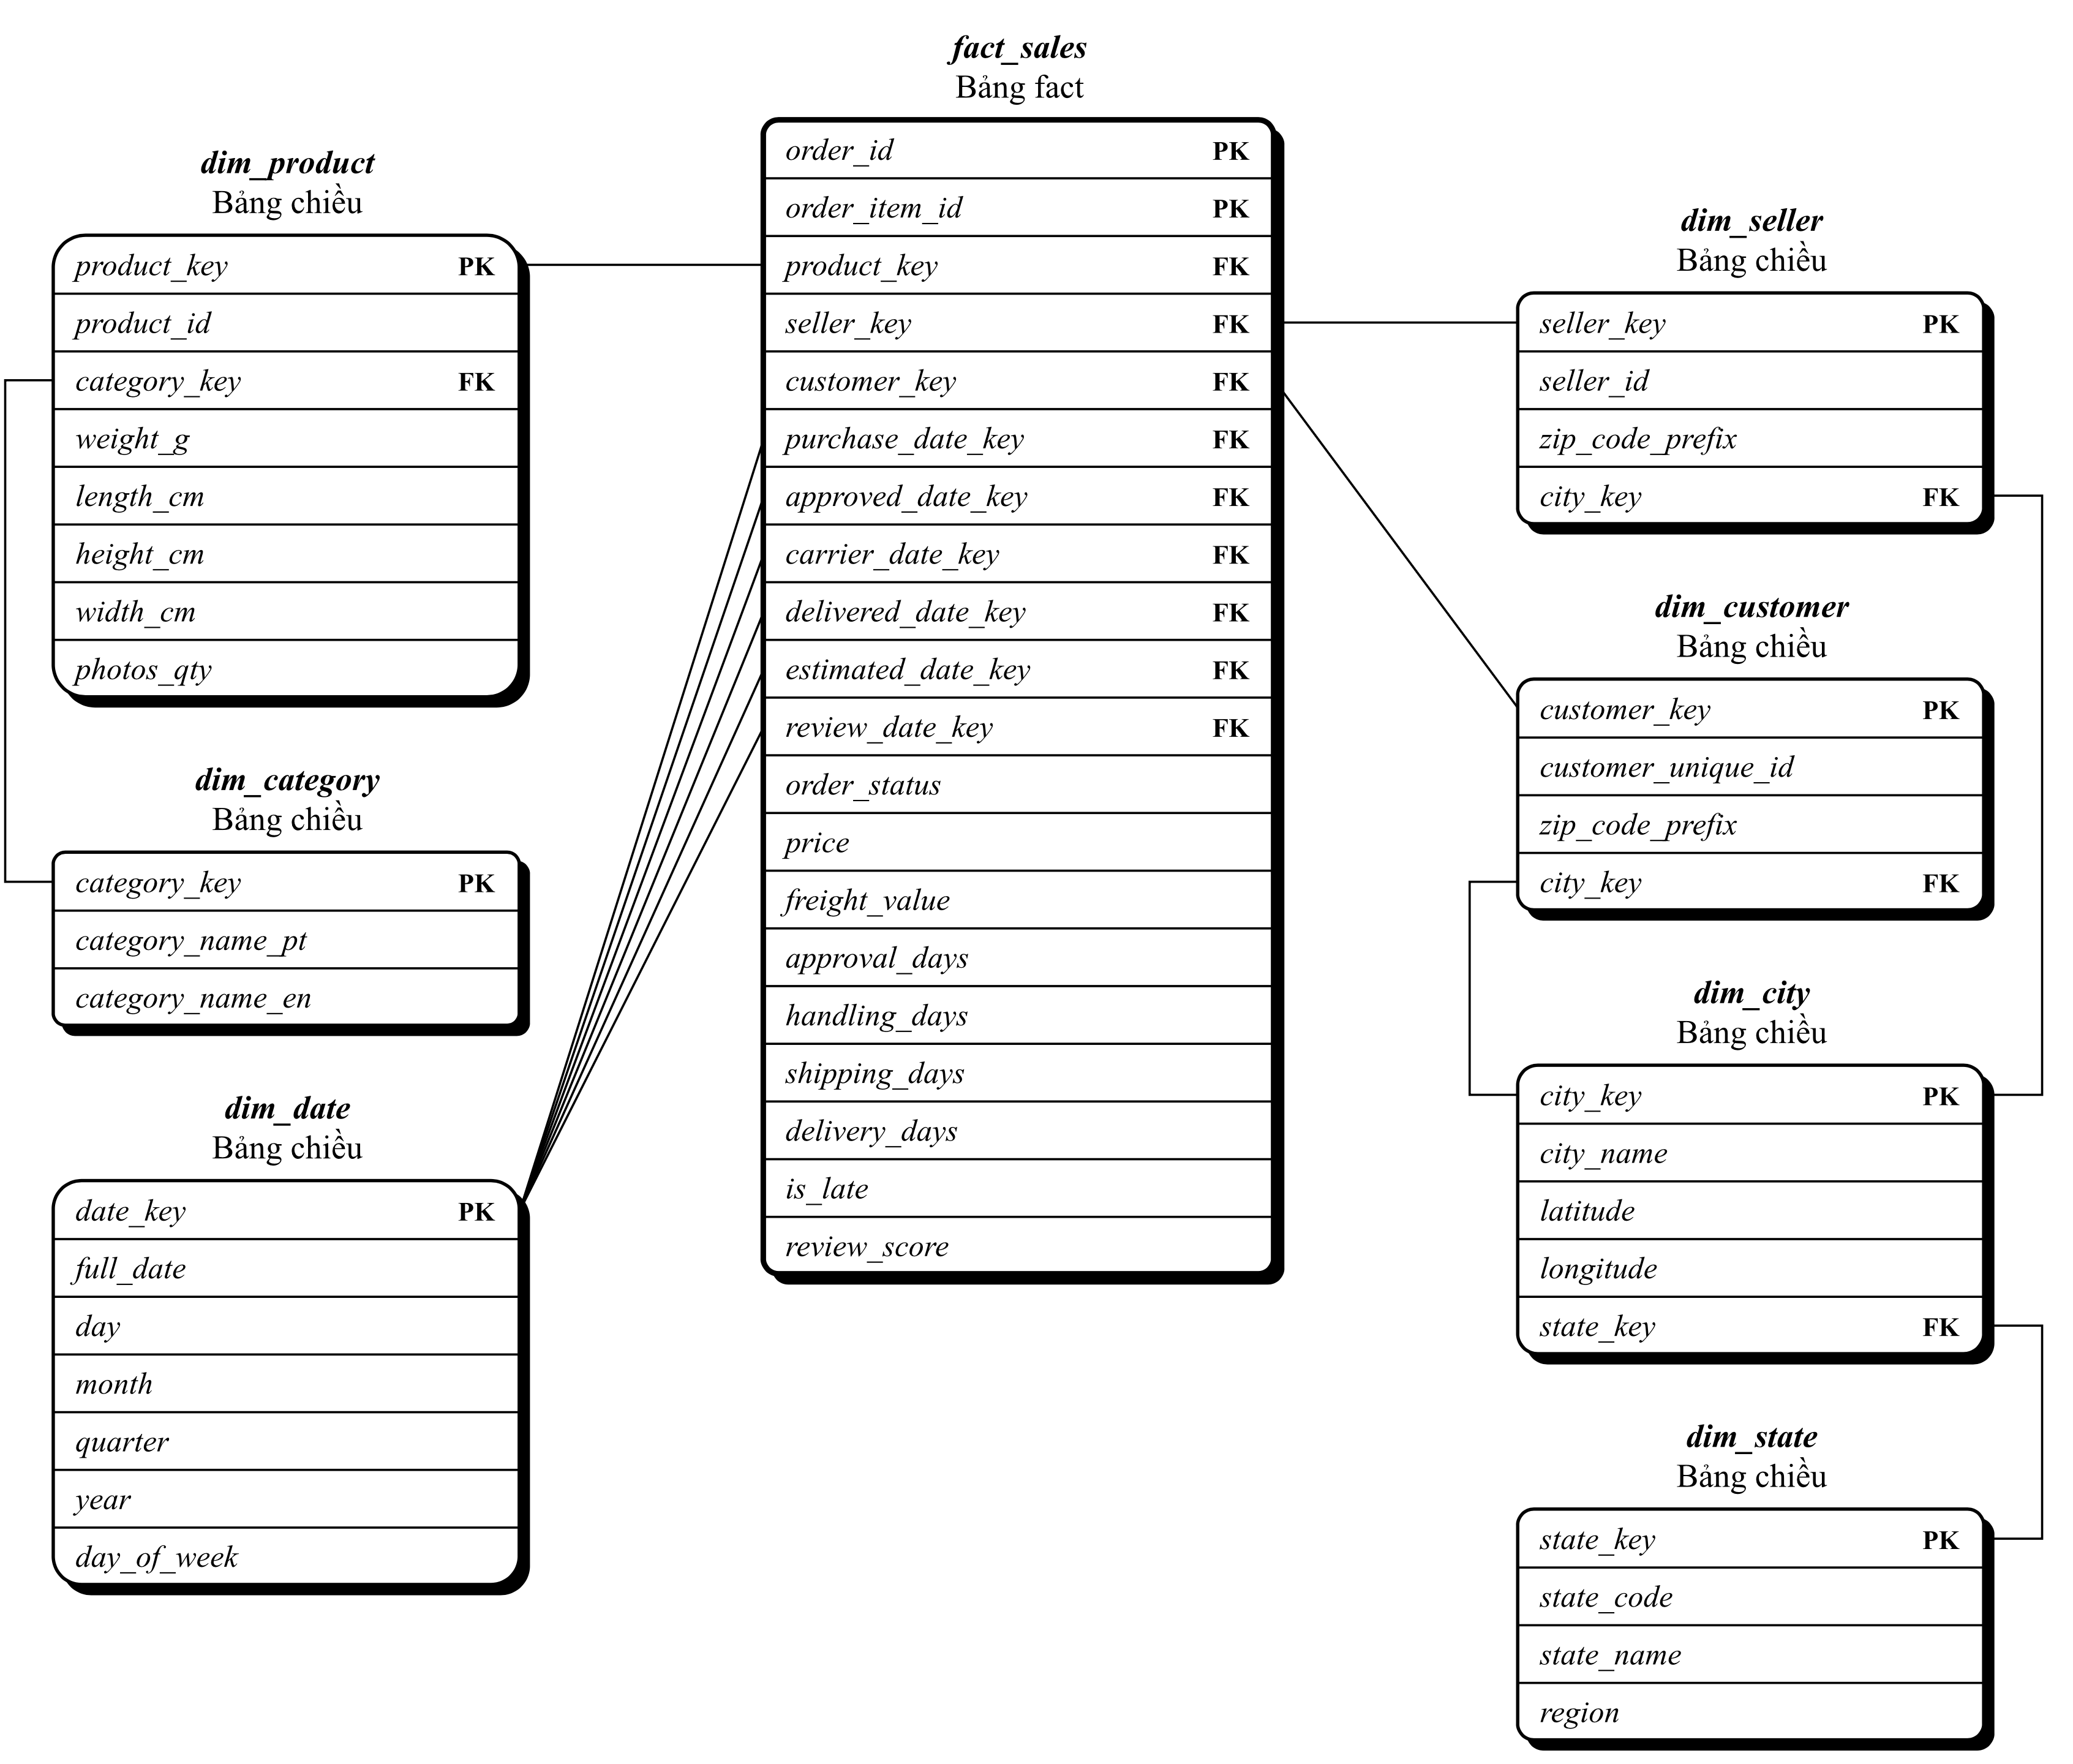
\includegraphics[width=\linewidth]{Pictures/schema-snowflake.png}
\caption{Sơ đồ snowflake schema của Data Mart}
\label{fig:schema}
\end{figure}

% !TeX root = ../../main.tex
\subsection{Thiết kế quy trình ETL}
\subsubsection{Tổng quan quy trình ETL}

ETL đưa dữ liệu từ nguồn vào kho qua ba bước trích xuất (Extract), biến đổi (Transform) và nạp (Load); dữ liệu được xử lý ở khu vực staging nằm giữa nguồn và kho trước khi vào kho. Hình~\ref{fig:etl} là luồng ETL của hệ thống.

% !TeX root = ../../main.tex
% Luồng ETL
\begin{figure}[H]
\centering
\resizebox{\linewidth}{!}{%
\begin{tikzpicture}[
    stage/.style={dwbox=#1, text width=3.3cm, minimum height=1.55cm},
    store/.style={dwdb=#1, text width=2.7cm, font=\footnotesize},
    num/.style={circle, fill=#1, text=white, font=\scriptsize\bfseries, inner sep=0pt, minimum size=13pt}]
\node[draw=dwLine, fill=white, line width=0.5pt, text width=2.6cm, align=center, font=\footnotesize, minimum height=1.4cm] (src) at (0,0)
  {\textbf{Dữ liệu nguồn}\\[-1pt]{\scriptsize 9 tập tin CSV và\\2 bảng tham chiếu}};
\node[stage=dwBlue] (ex) at (4.1,0)
  {\textbf{Extract}\\[-1pt]{\scriptsize \texttt{extract.py}: kiểm tra tiêu đề, \texttt{COPY}, đối chiếu số dòng}};
\node[store=dwYellow] (raw) at (8.3,0) {\textbf{Bảng thô}\\[-1pt]{\scriptsize\texttt{raw\_*}, \texttt{ref\_*}}\\[-1pt]{\scriptsize kiểu chuỗi}};
\node[stage=dwViolet] (tr) at (8.3,-2.75)
  {\textbf{Transformation}\\[-1pt]{\scriptsize \texttt{10\_transform.sql}: làm sạch, ánh xạ, tích hợp, quy tắc nghiệp vụ}};
\node[store=dwYellow] (stg) at (4.1,-2.75) {\textbf{Bảng đã làm sạch}\\[-1pt]{\scriptsize\texttt{stg\_*}}};
\node[stage=dwAqua] (ld) at (0,-5.5)
  {\textbf{Load} (một giao dịch)\\[-1pt]{\scriptsize tạo lại Data Mart, nạp bảng chiều rồi bảng fact}};
\node[store=dwBlue] (dm) at (4.1,-5.5) {\textbf{Data Mart}\\[-1pt]{\scriptsize\texttt{fact\_sales}}\\[-1pt]{\scriptsize + 7 bảng chiều}};
\node[stage=dwOrange] (dq) at (8.3,-5.5)
  {\textbf{Kiểm tra chất lượng}\\[-1pt]{\scriptsize \texttt{40\_dq\_checks.sql}: 20 tiêu chí đối soát}};
\node[dwdb=dwAqua, text width=2.5cm, font=\footnotesize] (meta) at (12.6,-2.75)
  {\textbf{Metadata}\\[1pt]{\scriptsize\texttt{etl\_run\_log}\\\texttt{rejected\_record}\\\texttt{dq\_result}}};
\foreach \n/\c/\l in {ex/dwBlue/1, tr/dwViolet/2, ld/dwAqua/3, dq/dwOrange/4}
  \node[num=\c] at (\n.north west) {\l};
\draw[dwarrow] (src) -- (ex);
\draw[dwarrow] (ex) -- (raw);
\draw[dwarrow] (raw) -- (tr);
\draw[dwarrow] (tr) -- (stg);
\draw[dwarrow, rounded corners=3pt] (stg.south) -- ++(0,-0.55) -| (ld.north);
\draw[dwarrow] (ld) -- (dm);
\draw[dwarrow] (dm) -- (dq);
\draw[dwdash, rounded corners=3pt] (ex.north) -- ++(0,0.75) -| (meta.north);
\draw[dwdash] (tr.east) -- node[dwlabel, above] {ghi nhật ký} (meta.west);
\draw[dwdash, rounded corners=3pt] (dq.east) -| (meta.south);
\draw[dwdash, rounded corners=3pt] (ld.south) -- ++(0,-0.45) -| ([xshift=0.7cm]meta.south);
\end{tikzpicture}}
\caption{Sơ đồ luồng ETL: bốn giai đoạn và các bảng trung gian; nét đứt là luồng ghi nhật ký vào kho metadata}
\label{fig:etl}
\end{figure}


Quy trình được viết bằng Python, còn phần biến đổi được viết bằng SQL và chạy ngay trong PostgreSQL. Khu vực staging là một schema riêng (\code{staging}) trong cùng cơ sở dữ liệu với Data Mart. Quy trình gồm bốn giai đoạn chạy lần lượt: Extract, Transformation, Load và kiểm tra chất lượng; giai đoạn nào cũng ghi kết quả vào nhật ký ETL để theo dõi và truy vết.

Hệ thống dùng ETL chứ không dùng ELT. Với ELT, dữ liệu được nạp vào kho trước rồi mới biến đổi, nghĩa là sẽ có lúc dữ liệu chưa sạch nằm trong kho và có thể bị ai đó dùng nhầm. Với ETL, Data Mart chỉ chứa dữ liệu đã qua làm sạch, còn dữ liệu thô nằm riêng trong staging.

\subsubsection{Extract -- Trích xuất dữ liệu}

Ở bước Extract, chín tập tin CSV của Olist (Bảng~\ref{tab:nguon}) được nạp nguyên trạng vào các bảng thô trong schema \code{staging}, tên có tiền tố \code{raw\_}, ví dụ \code{raw\_orders}, \code{raw\_order\_items}. Hai bảng tham chiếu do nhóm bổ sung, gồm bảng gán 27 bang vào vùng và bảng dịch hai ngành hàng còn thiếu, cũng được nạp vào staging với tiền tố \code{ref\_}.

Mọi cột ở bảng thô đều có kiểu chuỗi và chưa qua bất kỳ biến đổi nào. Cách làm này có hai lợi ích: một giá trị sai định dạng không làm hỏng cả lần nạp, và nếu bước sau lỗi thì có thể chạy lại từ bảng thô mà không cần đọc lại tập tin. Các tập tin được đọc theo bảng mã UTF-8; riêng \code{product\_category\_name\_translation} có ký tự đánh dấu thứ tự byte (BOM) ở đầu tập tin cần bỏ đi. Mã bưu chính được giữ ở dạng chuỗi để không mất số 0 ở đầu, ví dụ \code{01037}. Sau khi nạp, số dòng của từng bảng thô được so với số dòng trong Bảng~\ref{tab:nguon}, chẳng hạn 99.441 dòng đơn hàng và 112.650 dòng sản phẩm trong đơn.

\subsubsection{Transformation -- Biến đổi dữ liệu}

Bước transformation biến dữ liệu thô thành dữ liệu sạch và nhất quán, sẵn sàng nạp vào Data Mart; công việc gồm làm sạch, ánh xạ dữ liệu và áp dụng quy tắc nghiệp vụ. Kết quả được lưu vào các bảng đã làm sạch trong schema \code{staging}, tên có tiền tố \code{stg\_}.

\paragraph{Làm sạch dữ liệu}

Bước này hiện thực các quy tắc tiền xử lý đã xác định từ kết quả khám phá dữ liệu ở Bảng~\ref{tab:quytac} (mục~\ref{sec:tienxuly}). Mỗi quy tắc là một câu lệnh SQL chạy trên bảng thô; bản ghi nào bị loại hoặc bị sửa đều được ghi lại cùng lý do để truy vết về sau.

\paragraph{Ánh xạ và tích hợp dữ liệu}

Phần ánh xạ thống nhất kiểu dữ liệu và tên gọi: cột thời gian chuyển sang kiểu \code{timestamp}, giá và phí vận chuyển sang số thập phân, điểm đánh giá sang số nguyên; tên cột viết sai chính tả như \code{product\_name\_lenght} được sửa thành \code{product\_name\_length}.

Phần tích hợp xử lý ba chỗ mà các bảng nguồn không khớp nhau. Mã \code{customer\_id} theo từng đơn được quy về \code{customer\_unique\_id}, để mỗi khách hàng thật chỉ có một dòng trong bảng chiều khách hàng. Thành phố của khách hàng và người bán được gộp thành một danh sách duy nhất theo cặp (tên thành phố, mã bang); tọa độ của mỗi thành phố là trung bình tọa độ các điểm \code{geolocation} cùng tên và cùng bang. Cuối cùng, tên ngành hàng tiếng Bồ Đào Nha được nối với bảng dịch để có tên tiếng Anh.

\paragraph{Quy tắc nghiệp vụ và trường dẫn xuất}

Bốn khoảng thời gian \code{approval\_days}, \code{handling\_days}, \code{shipping\_days} và \code{delivery\_days} được tính bằng hiệu giữa hai mốc thời gian (gồm cả giờ, phút, giây) rồi quy đổi ra ngày, làm tròn hai chữ số thập phân; ví dụ 5 ngày 8 giờ được ghi là 5,34 ngày. Cờ \code{is\_late} bằng 1 khi ngày nhận hàng sau ngày giao dự kiến (so theo ngày) và bằng 0 trong trường hợp ngược lại; cờ chỉ được tính cho đơn đã có ngày nhận hàng. Mỗi bang được gán vào một trong năm vùng Norte, Nordeste, Centro-Oeste, Sudeste và Sul. Doanh thu hàng hóa chỉ tính từ giá bán của dòng sản phẩm, không gồm phí vận chuyển; trạng thái đơn hàng được giữ trong bảng fact để người dùng tự lọc đơn đã giao hay loại đơn bị hủy khi cần.

\subsubsection{Load -- Nạp dữ liệu}

Dữ liệu sạch được nạp từ staging vào Data Mart theo thứ tự từ bảng cha đến bảng con: \code{dim\_date}, \code{dim\_state}, \code{dim\_city}, \code{dim\_category}, \code{dim\_product}, \code{dim\_customer}, \code{dim\_seller}, rồi mới đến bảng fact. Như vậy, khi một bảng được nạp thì mọi bảng mà nó tham chiếu đã có dữ liệu. Khi nạp bảng fact, mỗi mã gốc như \code{product\_id}, \code{seller\_id}, \code{customer\_unique\_id} và mỗi mốc thời gian được tra sang surrogate key tương ứng; mã nào không tìm thấy được gán về bản ghi không xác định.

Vì dữ liệu nguồn là một tập lịch sử cố định, hệ thống dùng hình thức nạp toàn bộ (full load): mỗi lần chạy, Data Mart được xóa và nạp lại từ đầu. Toàn bộ bước Load nằm trong một giao dịch (transaction); nếu có lỗi, giao dịch bị hủy và Data Mart giữ nguyên dữ liệu của lần chạy trước, không nạp dở dang hay trùng dữ liệu. Khi nguồn dữ liệu phát sinh liên tục, quy trình có thể chuyển sang nạp tăng dần (incremental load) dựa trên thời điểm mua của đơn hàng.

Chỉ mục được tạo trên các khóa ngoại của bảng fact và trên \code{order\_id}, để tăng tốc phép kết nối và các truy vấn gom theo đơn hàng. Với quy mô hiện tại, nhóm chưa cần phân vùng (partition) bảng fact.

\subsubsection{Kiểm tra chất lượng và đối soát số liệu}

Sau mỗi lần chạy, hệ thống tự kiểm tra xem số liệu trong Data Mart có khớp với nguồn hay không. Bảng~\ref{tab:doisoat} là các tiêu chí đối soát cùng giá trị kỳ vọng; giá trị kỳ vọng được tính trực tiếp từ các tập tin CSV, độc lập với quy trình ETL.

\begin{table}[H]
\centering
\small\setstretch{1.1}
\caption{Tiêu chí đối soát số liệu sau khi chạy ETL}
\label{tab:doisoat}
\begin{tabularx}{\linewidth}{|>{\raggedright\arraybackslash}X|P{4.4cm}|}
\hline
\textbf{Tiêu chí đối soát} & \textbf{Giá trị kỳ vọng}\\ \hline
Số dòng của bảng fact so với số dòng sản phẩm trong đơn của nguồn & 112.650 dòng\\ \hline
Số đơn hàng phân biệt trong bảng fact & 98.666 đơn\\ \hline
Tổng giá bán & Khoảng 13,59 triệu BRL\\ \hline
Tổng phí vận chuyển & Khoảng 2,25 triệu BRL\\ \hline
Số khóa ngoại không tìm thấy bản ghi tương ứng trong bảng chiều & 0\\ \hline
Tỷ lệ giao trễ tính trên đơn hàng phân biệt & 6,77\%\\ \hline
Điểm đánh giá trung bình tính trên đơn hàng phân biệt & Xấp xỉ 4,1 điểm\\ \hline
\end{tabularx}
\end{table}

Số bản ghi bị loại hoặc bị sửa ở bước transformation, cùng lý do, cũng được ghi vào nhật ký ETL. Nếu một tiêu chí không đạt, lần chạy bị đánh dấu thất bại để được kiểm tra lại trước khi dữ liệu được dùng.

\subsubsection{Quản lý metadata}

Metadata là ``dữ liệu về dữ liệu'', mô tả số liệu trong kho chứ không phải bản thân số liệu. Metadata được lưu trong schema \code{meta} trên PostgreSQL (mục~\ref{sec:kientruc}) và gồm ba phần:
\begin{itemize}
    \item \textbf{Từ điển dữ liệu} (\code{data\_dictionary}) cho biết \emph{cột này là gì}: tên, kiểu, ý nghĩa nghiệp vụ và đơn vị tính của từng cột trong Data Mart.
    \item \textbf{Nguồn gốc dữ liệu} (\code{data\_lineage}) cho biết \emph{cột này từ đâu ra}: tập tin, cột nguồn và quy tắc biến đổi, giúp lần ngược về nguồn khi gặp con số bất thường.
    \item \textbf{Nhật ký ETL} cho biết \emph{lần nạp có ổn không}. \code{etl\_run\_log} ghi mỗi bước của mỗi lần chạy (thời gian, số dòng vào, ra, bị loại, trạng thái, lỗi); \code{rejected\_record} lưu bản ghi bị loại hoặc bị sửa kèm lý do; \code{dq\_result} lưu kết quả đối soát. Đây là chức năng giám sát (Monitoring) trong kiến trúc hệ thống.
\end{itemize}


\clearpage
% !TeX root = ../main.tex
\section{Hiện thực hệ thống}\label{sec:hienthuc}

Phần này trình bày cách hiện thực thiết kế ở mục~\ref{sec:thietke}: môi trường triển khai, quy trình ETL chạy trên toàn bộ dữ liệu nguồn, các truy vấn OLAP trên Data Mart và giao diện dashboard. Mọi con số và biểu đồ trong phần này được lấy từ lần chạy thực tế của hệ thống; các biểu đồ được sinh tự động bằng chương trình \code{src/report/make\_figures.py} đọc trực tiếp từ cơ sở dữ liệu, nên có thể tạo lại sau mỗi lần nạp dữ liệu.

% !TeX root = ../../main.tex
\subsection{Môi trường và cấu trúc mã nguồn}\label{sec:trienkhai}

Hệ thống chạy trên localhost (máy cá nhân). Cơ sở dữ liệu được đặt trong một container Docker, nhờ vậy mọi người dùng cùng một phiên bản PostgreSQL và cùng cấu hình mà không phải cài đặt riêng. Bảng~\ref{tab:congnghe} liệt kê các thành phần và công nghệ sử dụng.

\begin{table}[H]
\centering
\small\setstretch{1.1}
\caption{Thành phần và công nghệ của hệ thống}
\label{tab:congnghe}
\begin{tabularx}{\linewidth}{|P{3.4cm}|P{4.2cm}|>{\raggedright\arraybackslash}X|}
\hline
\textbf{Thành phần} & \textbf{Công nghệ} & \textbf{Vai trò}\\ \hline
Cơ sở dữ liệu & PostgreSQL 16 (Docker) & Lưu khu vực staging, Data Mart, kho metadata và kết quả DSS trong bốn schema \code{staging}, \code{dm}, \code{meta}, \code{dss}\\ \hline
Quy trình ETL & Python 3, psycopg 3, SQL & Python điều phối các bước và ghi nhật ký; các phép biến đổi viết bằng SQL và chạy trong cơ sở dữ liệu\\ \hline
OLAP & SQL trên PostgreSQL (ROLAP) & Thư viện truy vấn \code{50\_olap\_queries.sql} và chương trình chạy, đo thời gian \code{run\_olap.py}\\ \hline
Biểu đồ trong báo cáo & Python, matplotlib & Sinh lại toàn bộ biểu đồ dữ liệu từ cơ sở dữ liệu\\ \hline
Hệ hỗ trợ quyết định & Python, pandas, scikit-learn & Xây dựng đặc trưng, huấn luyện và chấm điểm mô hình, ghi kết quả vào schema \code{dss}\\ \hline
Dashboard & Python, Streamlit 1.67, Plotly 7.1, SQLAlchemy & Giao diện web cho từng nhóm người dùng, truy vấn trực tiếp Data Mart; ghi quyết định của người vận hành vào \code{dss.decision\_log}\\ \hline
\end{tabularx}
\end{table}

Mã nguồn được chia thư mục theo từng thành phần của kiến trúc. Thư mục \code{data} chứa chín tập tin CSV gốc (\code{data/raw}) và hai bảng tham chiếu do nhóm bổ sung (\code{data/reference}). Thư mục \code{src/sql} chứa các tập tin SQL đánh số theo thứ tự chạy: tạo schema (\code{00}-\code{05}), biến đổi (\code{10}), nạp bảng chiều (\code{20}), nạp bảng fact (\code{30}), kiểm tra chất lượng (\code{40}) và thư viện truy vấn OLAP (\code{50}). Phần Python nằm trong \code{src/etl} (điều phối ETL), \code{src/olap} (chạy truy vấn OLAP), \code{src/dss} (hệ hỗ trợ quyết định), \code{src/dashboard} (dashboard) và \code{src/report} (sinh biểu đồ).

Để dựng hệ thống trên một máy mới, chỉ cần ba bước: khởi động cơ sở dữ liệu bằng \code{docker compose -f src/docker-compose.yml up -d}, cài các thư viện trong \code{src/requirements.txt}, rồi chạy \code{python -m src.etl.run\_etl --init}. Lệnh cuối tạo toàn bộ schema, bảng và thực hiện một lần ETL đầy đủ. Thông tin kết nối cơ sở dữ liệu nằm trong tập tin \code{.env} và không được đưa lên kho mã nguồn.

% !TeX root = ../../main.tex
\subsection{Hiện thực quy trình ETL}\label{sec:hienthucetl}

Quy trình ETL được hiện thực đúng bốn giai đoạn đã thiết kế ở Hình~\ref{fig:etl}. Chương trình \code{run\_etl.py} gọi lần lượt từng giai đoạn; mỗi bước để lại một dòng trong bảng nhật ký \code{meta.etl\_run\_log} gồm thời điểm bắt đầu, kết thúc, số dòng và trạng thái. Bảng~\ref{tab:etlbuoc} là kết quả của một lần chạy đầy đủ.

\begin{table}[H]
\centering
\small\setstretch{1.1}
\caption{Kết quả một lần chạy ETL đầy đủ}
\label{tab:etlbuoc}
\begin{tabularx}{\linewidth}{|P{2.9cm}|P{4.6cm}|>{\raggedright\arraybackslash}X|P{1.6cm}|}
\hline
\textbf{Giai đoạn} & \textbf{Tập tin} & \textbf{Kết quả} & \textbf{Thời gian}\\ \hline
Extract & \code{extract.py} & Nạp 11 tập tin (9 tập tin nguồn và 2 bảng tham chiếu) vào staging, tổng cộng 1.550.922 dòng dữ liệu nguồn; số dòng từng bảng khớp với tập tin & 1,0 giây\\ \hline
Transformation & \code{10\_transform.sql} & Tạo 11 bảng đã làm sạch \code{stg\_*}; ghi nhận 775 đơn hàng bị loại và 1.458 bản ghi được sửa & 4,5 giây\\ \hline
Load & \code{02\_datamart\_ddl.sql}\newline \code{20\_load\_dims.sql}\newline \code{30\_load\_fact.sql}\newline \code{05\_metadata\_seed.sql} & Tạo lại Data Mart và nạp 7 bảng chiều, 112.650 dòng bảng fact cùng từ điển dữ liệu và nguồn gốc dữ liệu & 3,1 giây\\ \hline
Kiểm tra chất lượng & \code{40\_dq\_checks.sql} & 20/20 tiêu chí đối soát đạt & 0,1 giây\\ \hline
\multicolumn{3}{|l|}{\textbf{Tổng thời gian một lần chạy}} & \textbf{8,7 giây}\\ \hline
\end{tabularx}
\end{table}

Ở bước Extract, mỗi tập tin được nạp thẳng vào bảng thô bằng lệnh \code{COPY} của PostgreSQL. Trước khi nạp, chương trình so dòng tiêu đề của tập tin với cấu trúc bảng thô; sau khi nạp, so số dòng với số dòng kỳ vọng. Chỉ cần lệch một trong hai là quy trình dừng. Nhờ dùng \code{COPY} thay vì chèn từng dòng, tập \code{geolocation} hơn một triệu dòng được nạp trong chưa đầy một giây.

Các quy tắc ở Bảng~\ref{tab:quytac} được viết thành câu lệnh SQL xử lý trên cả bảng một lần, thay vì đọc từng dòng ra Python để xử lý. Chẳng hạn, việc chuẩn hóa tên thành phố được viết thành hàm \code{staging.norm\_city}: chuyển chữ thường, bỏ dấu bằng extension \code{unaccent}, cắt phần mã bang thừa. Việc chọn một đánh giá cho mỗi đơn dùng hàm cửa sổ \code{ROW\_NUMBER()}. Đoạn mã dưới đây là cách tính thời gian chuẩn bị hàng và cờ giao trễ; khoảng thời gian âm do mốc sai thứ tự được để trống đúng như quy tắc đã đặt ra.

\begin{lstlisting}[style=SQLStyle]
CASE WHEN carrier_ts >= approved_ts
     THEN ROUND(EXTRACT(EPOCH FROM carrier_ts - approved_ts) / 86400.0, 2) END AS handling_days,
CASE WHEN order_status = 'delivered' AND delivered_ts IS NOT NULL
     THEN (delivered_ts::date > estimated_ts::date)::int::smallint END       AS is_late
\end{lstlisting}

Surrogate key được sinh bằng \code{ROW\_NUMBER()} sắp theo mã gốc, nên các lần nạp toàn bộ liên tiếp luôn cho cùng một khóa với cùng một đối tượng. Toàn bộ giai đoạn Load, từ xóa và tạo lại Data Mart đến nạp xong bảng fact, chạy trong một giao dịch. PostgreSQL hỗ trợ giao dịch cho cả câu lệnh định nghĩa dữ liệu, nên chỉ một câu lệnh lỗi là cả giai đoạn bị hủy và Data Mart quay về đúng dữ liệu của lần chạy trước.

\subsubsection{Kết quả xử lý chất lượng dữ liệu}

Các bản ghi bị loại hoặc bị sửa được ghi vào bảng \code{meta.rejected\_record} kèm lý do. Bảng~\ref{tab:etlxuly} tổng hợp kết quả của lần chạy.

\begin{table}[H]
\centering
\small\setstretch{1.1}
\caption{Các bản ghi bị loại hoặc bị sửa trong bước transformation}
\label{tab:etlxuly}
\begin{tabularx}{\linewidth}{|>{\raggedright\arraybackslash}X|P{3.3cm}|P{2.2cm}|}
\hline
\textbf{Vấn đề} & \textbf{Xử lý} & \textbf{Số bản ghi}\\ \hline
Thời điểm bàn giao vận chuyển trước thời điểm duyệt & Để trống \code{handling\_days} & 1.359 đơn\\ \hline
Đơn hàng không có dòng sản phẩm & Không nạp vào bảng fact & 775 đơn\\ \hline
Tên thành phố của người bán không chuẩn & Chuẩn hóa tên & 68 người bán\\ \hline
Thời điểm bàn giao vận chuyển sau thời điểm nhận hàng & Để trống \code{shipping\_days} & 23 đơn\\ \hline
Trạng thái đã giao nhưng thiếu thời điểm nhận hàng & Không tính chỉ số giao hàng & 8 đơn\\ \hline
\end{tabularx}
\end{table}

Tên thành phố của người bán cần thêm một bước đối chiếu. Nhiều tên là dạng viết tắt hoặc viết sai: \code{sp / sp} sau khi cắt phần sau dấu ``/'' chỉ còn \code{sp}, \code{sbc/sp} còn \code{sbc} (viết tắt của São Bernardo do Campo), hay \code{sao pauo} thiếu một chữ. Vì vậy, nếu tên đã chuẩn hóa không có trong \code{geolocation} của bang tương ứng thì tên thành phố được lấy theo mã bưu chính. Quy tắc này gộp các tên viết khác nhau của cùng một thành phố, còn lại 4.341 thành phố và chỉ 34 người bán thuộc thành phố không có tọa độ; nó cũng sửa \code{balenario camboriu} thành \code{balneario camboriu} và đưa tên quận \code{vicente de carvalho} về đúng đô thị \code{guaruja}.

Các kết quả còn lại của bước làm sạch và tích hợp như sau. Tập \code{geolocation} còn 738.332 dòng sau khi bỏ 261.831 dòng trùng, rồi còn 738.299 dòng thuộc 19.010 tiền tố mã bưu chính sau khi bỏ các điểm ngoài lãnh thổ. Có 79 thành phố không có tọa độ vì mã bưu chính của chúng không xuất hiện trong \code{geolocation}. 99.441 mã \code{customer\_id} được quy về 96.096 khách hàng thật, và 99.224 dòng đánh giá được rút về 98.673 đánh giá chính thức.

\subsubsection{Kết quả đối soát số liệu}

Sau giai đoạn Load, chương trình chạy 20 tiêu chí đối soát và ghi kết quả vào \code{meta.dq\_result}. Bảng~\ref{tab:etldoisoat} đặt giá trị kỳ vọng ở Bảng~\ref{tab:doisoat} cạnh giá trị thực tế trong Data Mart; tất cả đều khớp.

\begin{table}[H]
\centering
\small\setstretch{1.1}
\caption{Kết quả đối soát số liệu sau khi chạy ETL}
\label{tab:etldoisoat}
\begin{tabularx}{\linewidth}{|>{\raggedright\arraybackslash}X|P{3.2cm}|P{3.2cm}|}
\hline
\textbf{Tiêu chí} & \textbf{Kỳ vọng} & \textbf{Thực tế}\\ \hline
Số dòng bảng fact & 112.650 & 112.650\\ \hline
Số đơn hàng phân biệt trong bảng fact & 98.666 & 98.666\\ \hline
Tổng giá bán (BRL) & 13.591.643,70 & 13.591.643,70\\ \hline
Tổng phí vận chuyển (BRL) & 2.251.909,54 & 2.251.909,54\\ \hline
Tỷ lệ giao trễ trên đơn hàng phân biệt & 6,77\% & 6,77\%\\ \hline
Điểm đánh giá trung bình trên đơn hàng phân biệt & Xấp xỉ 4,1 & 4,105\\ \hline
Số dòng của \code{dim\_customer}, \code{dim\_product}, \code{dim\_seller} (kể cả bản ghi không xác định) & 96.097; 32.952; 3.096 & 96.097; 32.952; 3.096\\ \hline
Số dòng bảng fact tham chiếu sản phẩm, người bán, khách hàng hoặc ngày mua không xác định & 0 & 0\\ \hline
\end{tabularx}
\end{table}

Tính tin cậy của quy trình được kiểm tra thêm ở hai tình huống. Khi chạy ETL nhiều lần liên tiếp, số dòng và tổng tiền ở mọi bảng không đổi và cả 20 tiêu chí đều đạt ở mỗi lần. Để kiểm tra trường hợp lỗi, chương trình \code{verify\_rollback.py} chạy các bước Load rồi cố ý gây lỗi trước khi xác nhận giao dịch: ngay bên trong giao dịch, bảng fact đã bị xóa còn 0 dòng, nhưng sau khi giao dịch bị hủy, Data Mart trở lại đủ 112.650 dòng với tổng giá bán 13.591.643,70 BRL.

Một lần chạy ETL đầy đủ mất 8,7 giây, nên có thể nạp lại toàn bộ bất cứ lúc nào mà không cần cơ chế nạp tăng dần. Data Mart sau khi nạp chiếm khoảng 62 MB, trong đó bảng fact có 17 MB dữ liệu và 24 MB chỉ mục.

% !TeX root = ../../main.tex
\subsection{Phân tích OLAP trên Data Mart}\label{sec:olap}

Theo mô hình ROLAP đã chọn (mục~\ref{sec:kientruc}), khối dữ liệu chính là bảng fact \code{fact\_sales} cùng các bảng chiều, và mỗi phép toán OLAP là một truy vấn SQL dùng \code{GROUP BY}, \code{ROLLUP} hoặc \code{CUBE}. Tập tin \code{50\_olap\_queries.sql} có 14 truy vấn, mỗi truy vấn trả lời một nhu cầu ở Bảng~\ref{tab:quyetdinh}. Hai quy ước được áp dụng cho mọi truy vấn: thước đo theo đơn hàng (thời gian giao, cờ trễ, điểm đánh giá) luôn lấy từ view \code{dm.v\_order} để mỗi đơn chỉ được tính một lần (mục~\ref{sec:dodo}), và doanh thu không tính các đơn ở trạng thái \code{canceled} hay \code{unavailable}.

\subsubsection{Roll-up}

Phép roll-up tổng hợp doanh thu theo phân cấp Tháng $\rightarrow$ Quý $\rightarrow$ Năm. Chỉ với một câu lệnh \code{GROUP BY ROLLUP (year, quarter, month)}, PostgreSQL trả về cùng lúc dòng chi tiết theo tháng, dòng tổng theo quý, theo năm và dòng tổng toàn bộ.

\begin{lstlisting}[style=SQLStyle]
SELECT d.year, d.quarter, d.month,
       SUM(f.price) AS revenue, COUNT(DISTINCT f.order_id) AS orders
FROM dm.fact_sales f JOIN dm.dim_date d ON d.date_key = f.purchase_date_key
WHERE f.order_status NOT IN ('canceled', 'unavailable')
GROUP BY ROLLUP (d.year, d.quarter, d.month);
\end{lstlisting}

Bảng~\ref{tab:rollup} là kết quả ở mức quý và năm; Hình~\ref{fig:rollupthang} vẽ lại mức tháng trong giai đoạn 01/2017-08/2018.

\begin{table}[H]
\centering
\small\setstretch{1.1}
\caption{Kết quả roll-up doanh thu theo quý và năm}
\label{tab:rollup}
\begin{tabularx}{\linewidth}{|P{2.4cm}|>{\raggedleft\arraybackslash}X|>{\raggedleft\arraybackslash}X|>{\raggedleft\arraybackslash}X|}
\hline
\textbf{Kỳ} & \textbf{Doanh thu (BRL)} & \textbf{Số đơn} & \textbf{Giá trị đơn TB (BRL)}\\ \hline
Quý 1/2017 & 733.398,94 & 5.122 & 143,19\\ \hline
Quý 2/2017 & 1.286.918,78 & 9.222 & 139,55\\ \hline
Quý 3/2017 & 1.681.949,00 & 12.445 & 135,15\\ \hline
Quý 4/2017 & 2.406.225,55 & 17.586 & 136,83\\ \hline
\textbf{Năm 2017} & \textbf{6.108.492,27} & \textbf{44.375} & \textbf{137,66}\\ \hline
Quý 1/2018 & 2.764.402,78 & 20.979 & 131,77\\ \hline
Quý 2/2018 & 2.849.730,26 & 19.897 & 143,22\\ \hline
Quý 3/2018 (07-09/2018) & 1.727.049,37 & 12.655 & 136,47\\ \hline
\textbf{Năm 2018} & \textbf{7.341.182,41} & \textbf{53.531} & \textbf{137,14}\\ \hline
\textbf{Toàn bộ (2016-2018)} & \textbf{13.494.400,74} & \textbf{98.199} & \textbf{137,42}\\ \hline
\end{tabularx}
\end{table}

\begin{figure}[H]
\centering
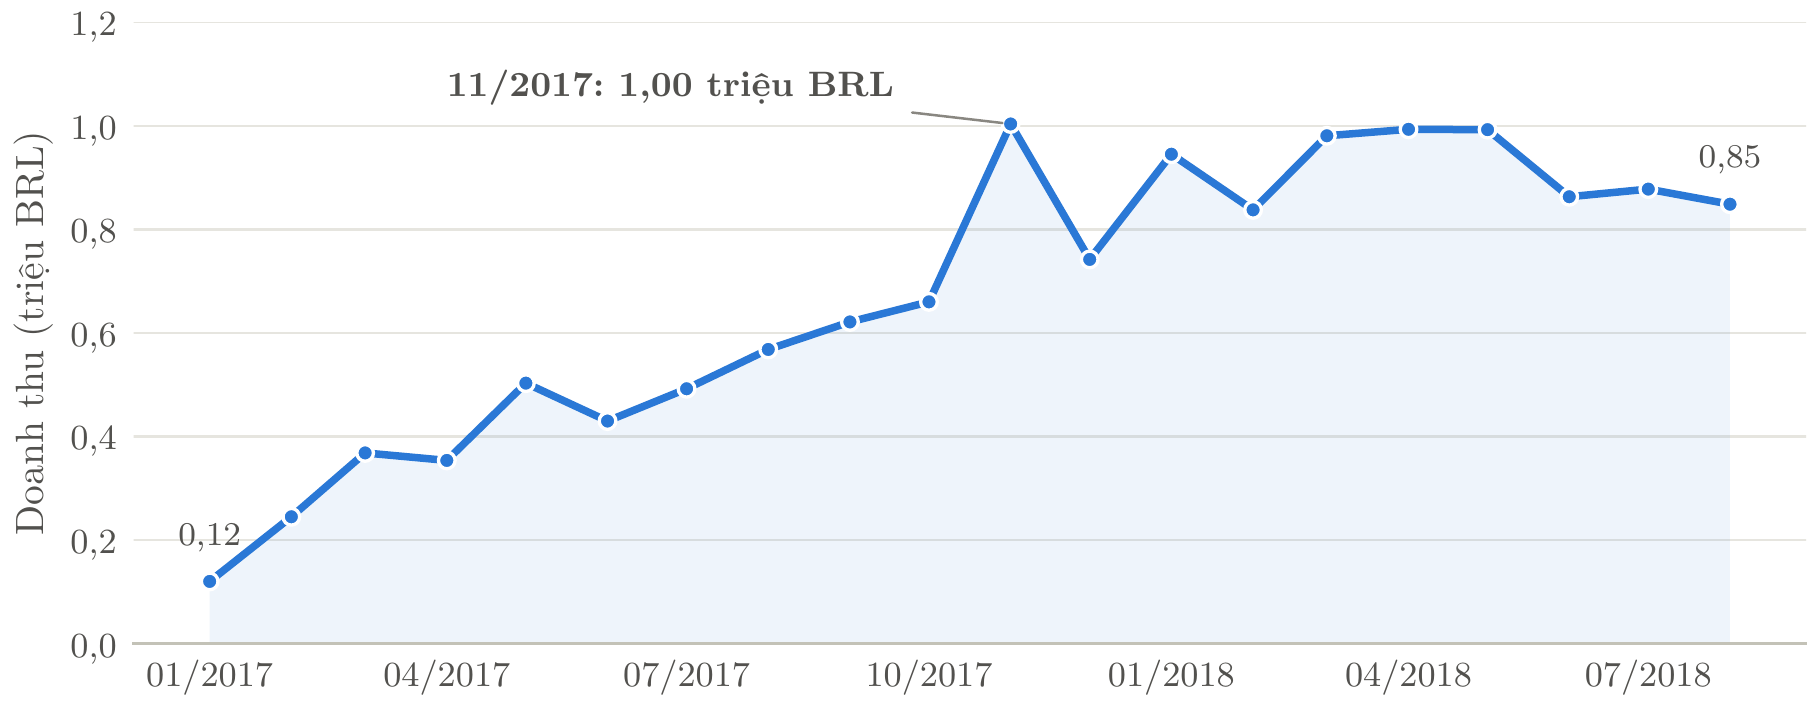
\includegraphics{Pictures/fig-olap-rollup-thang.png}
\caption{Doanh thu hàng hóa theo tháng, giai đoạn 01/2017-08/2018 (mức tháng của phép roll-up)}
\label{fig:rollupthang}
\end{figure}

Doanh thu tăng đều qua từng quý của năm 2017 và lên đỉnh vào tháng 11/2017 với 1,00 triệu BRL, rồi giảm mạnh ở tháng 12. Sang năm 2018, doanh thu mỗi quý đứng quanh mức 2,8 triệu BRL; quý 3/2018 thấp hơn chỉ vì dữ liệu dừng ở tháng 08/2018. Giá trị đơn trung bình hầu như không đổi, khoảng 137 BRL, nên có thể nói tăng trưởng của sàn đến từ số đơn hàng chứ không phải từ việc khách mua đơn lớn hơn.

\subsubsection{Drill-down}

Phép drill-down đi ngược chiều roll-up: từ vùng xuống bang rồi xuống thành phố của khách hàng, ở đây để tìm nơi giao trễ nhiều. Bảng~\ref{tab:drilldown} là mức vùng kèm một vài bang tiêu biểu; Hình~\ref{fig:drilldown} là mức bang đầy đủ, mỗi thanh được tô theo vùng mà bang đó thuộc về.

\begin{table}[H]
\centering
\small\setstretch{1.1}
\caption{Drill-down tỷ lệ giao trễ từ vùng xuống bang}
\label{tab:drilldown}
\begin{tabularx}{\linewidth}{|P{3.0cm}|>{\raggedleft\arraybackslash}X|>{\raggedleft\arraybackslash}X|>{\raggedleft\arraybackslash}X|}
\hline
\textbf{Vùng / Bang} & \textbf{Số đơn đã giao} & \textbf{Tỷ lệ trễ} & \textbf{Thời gian giao TB (ngày)}\\ \hline
Sudeste & 66.197 & 6,12\% & 10,8\\ \hline
\quad RJ & 12.351 & 12,11\% & 15,3\\ \hline
\quad SP & 40.499 & 4,49\% & 8,8\\ \hline
Sul & 13.812 & 5,90\% & 14,0\\ \hline
Centro-Oeste & 5.619 & 6,50\% & 15,0\\ \hline
Nordeste & 9.045 & 12,71\% & 20,0\\ \hline
\quad AL & 397 & 21,41\% & 24,5\\ \hline
\quad MA & 720 & 17,36\% & 21,5\\ \hline
Norte & 1.797 & 8,57\% & 22,6\\ \hline
\textbf{Toàn quốc} & \textbf{96.470} & \textbf{6,77\%} & \textbf{12,6}\\ \hline
\end{tabularx}
\end{table}

\begin{figure}[H]
\centering
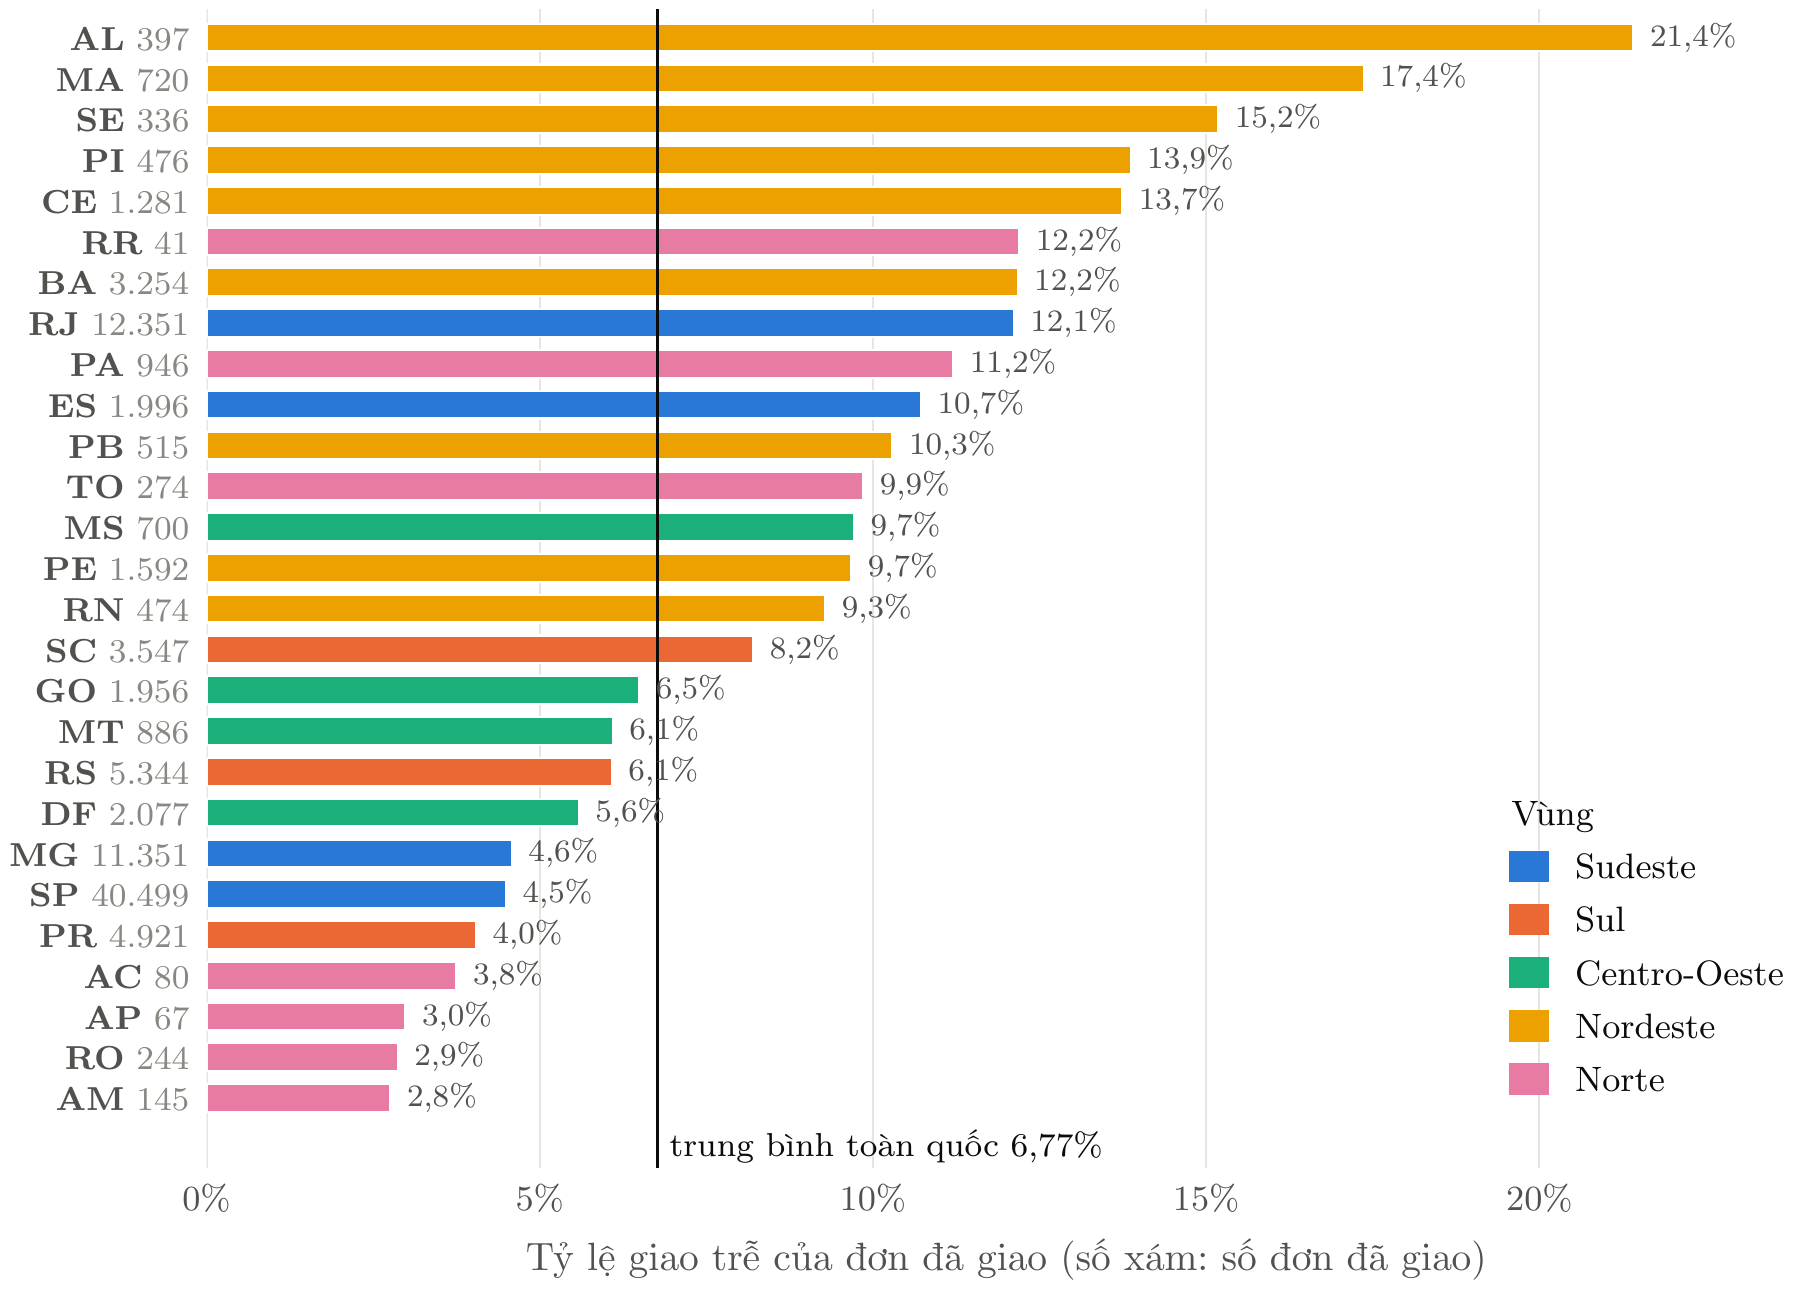
\includegraphics{Pictures/fig-olap-drilldown-bang.png}
\caption{Tỷ lệ giao trễ theo bang của khách hàng, tô màu theo vùng (mức bang của phép drill-down)}
\label{fig:drilldown}
\end{figure}

Ở mức vùng, Nordeste có tỷ lệ trễ 12,71\%, gần gấp đôi trung bình toàn quốc, và Hình~\ref{fig:drilldown} cho thấy gần như mọi bang của Nordeste đều nằm trên đường trung bình. Điều bất ngờ hơn chỉ lộ ra khi drill-down: Sudeste, vùng có tỷ lệ trễ thấp, lại chứa bang RJ với 12,11\%, gần gấp ba bang SP bên cạnh. Đi tiếp xuống thành phố của RJ, \code{sao goncalo} trễ 21,50\% trên 386 đơn, còn thành phố \code{rio de janeiro} là 10,72\% trên 6.597 đơn. Nếu chỉ nhìn ở mức vùng, nhà quản lý sẽ bỏ qua một điểm nóng giao trễ ở nơi có nhiều đơn hàng thứ hai cả nước.

Hình~\ref{fig:drilldown} cũng nhắc lại giới hạn đã nêu ở mục~\ref{sec:quanhe}: các bang nhỏ như RR (41 đơn) hay AP (67 đơn) có quá ít đơn để tỷ lệ trễ của chúng đáng tin.

\subsubsection{Slice và Dice}

Phép slice cố định một giá trị trên một chiều; ở đây là năm 2018 trên chiều thời gian, xem doanh thu theo vùng (Bảng~\ref{tab:slice}). Phép dice chọn một tập giá trị trên nhiều chiều cùng lúc; ở đây là quý 4/2017, ba bang SP, RJ, MG và năm ngành hàng có doanh thu cao nhất năm 2017 (Hình~\ref{fig:dice}).

\begin{table}[H]
\centering
\small\setstretch{1.1}
\caption{Kết quả slice năm 2018: doanh thu theo vùng}
\label{tab:slice}
\begin{tabularx}{\linewidth}{|P{3.8cm}|>{\raggedleft\arraybackslash}X|>{\raggedleft\arraybackslash}X|>{\raggedleft\arraybackslash}X|}
\hline
\textbf{Vùng} & \textbf{Doanh thu (BRL)} & \textbf{Số đơn} & \textbf{Tỷ trọng doanh thu}\\ \hline
Sudeste & 4.866.163,13 & 37.301 & 66,3\%\\ \hline
Sul & 1.047.635,66 & 7.394 & 14,3\%\\ \hline
Nordeste & 804.697,84 & 4.801 & 11,0\%\\ \hline
Centro-Oeste & 458.089,53 & 3.152 & 6,2\%\\ \hline
Norte & 164.596,25 & 883 & 2,2\%\\ \hline
\end{tabularx}
\end{table}

\begin{figure}[H]
\centering
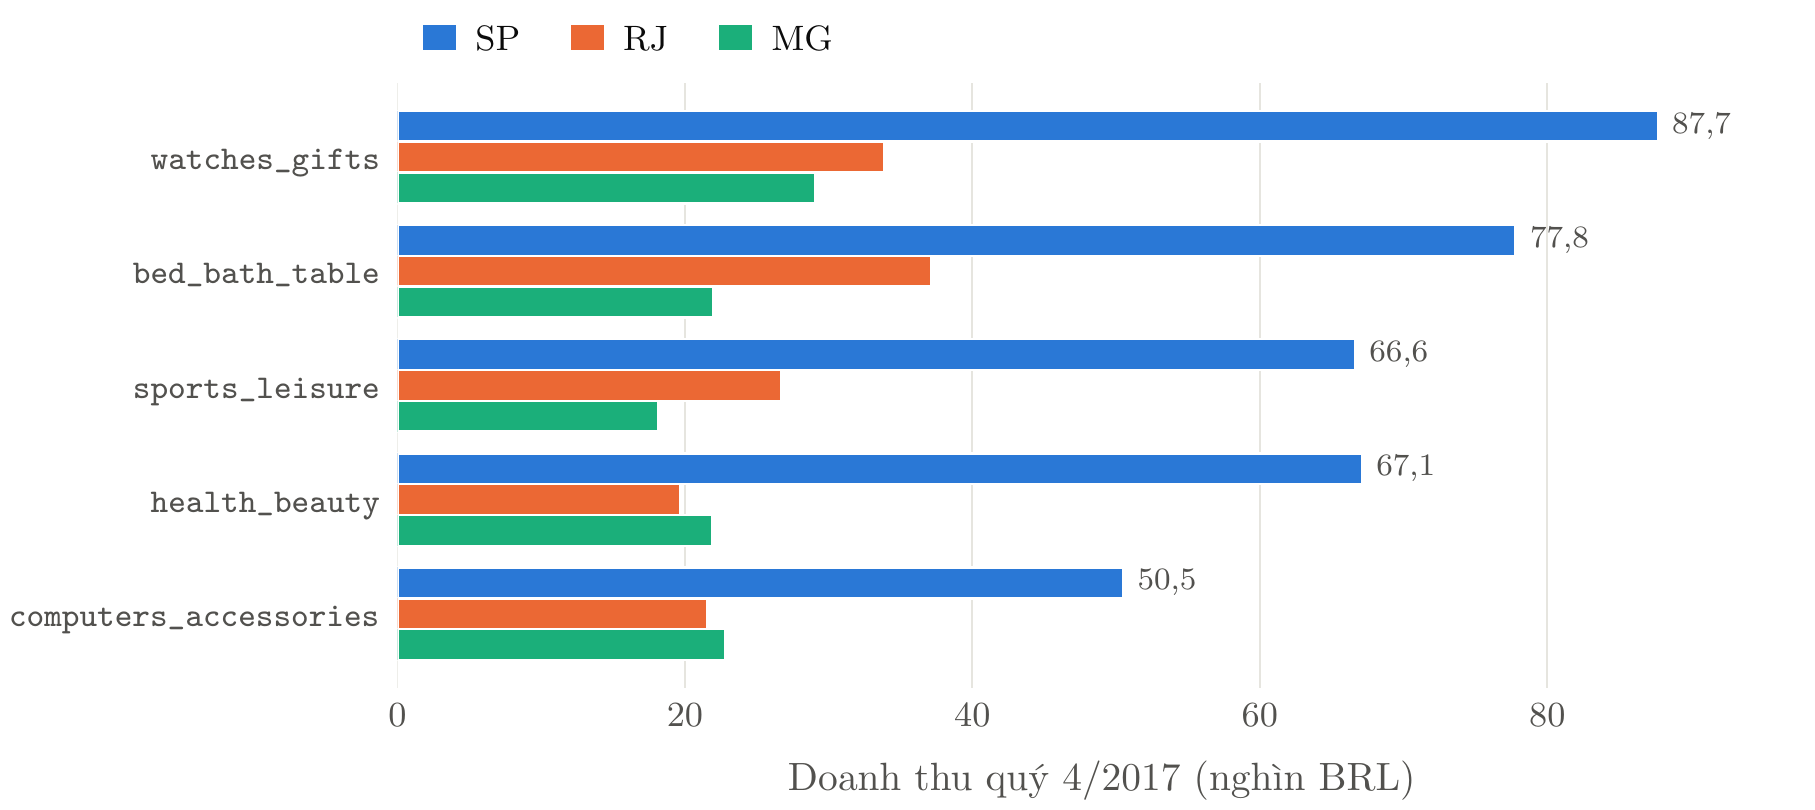
\includegraphics{Pictures/fig-olap-dice.png}
\caption{Kết quả dice: doanh thu quý 4/2017 của năm ngành hàng dẫn đầu năm 2017 tại các bang SP, RJ và MG}
\label{fig:dice}
\end{figure}

Năm 2018, riêng vùng Sudeste đã chiếm hai phần ba doanh thu. Trong mùa cao điểm quý 4/2017, SP dẫn đầu mọi ngành hàng như dự đoán, nhưng thứ tự ngành hàng thay đổi theo bang: \code{watches\_gifts} đứng đầu ở SP (87.690,54 BRL) và MG, trong khi ở RJ ngành bán chạy nhất là \code{bed\_bath\_table} (37.163,75 BRL). Vì vậy, thay vì áp dụng một chương trình khuyến mãi chung, nên chọn ngành hàng ưu tiên riêng cho từng bang.

\subsubsection{Pivot}

Phép pivot xoay chiều vùng từ dòng sang cột để so điểm đánh giá của từng ngành hàng giữa các vùng. Trong SQL, phép xoay được viết bằng hàm tổng hợp có điều kiện \code{AVG(...) FILTER (WHERE region = ...)}, mỗi vùng một cột. Hình~\ref{fig:pivot} là kết quả cho mười ngành hàng có nhiều đơn nhất. Các dòng được xếp theo điểm trung bình của ngành trên toàn quốc, tính trên mọi đơn của ngành và không hiển thị trong hình, tăng dần từ trên xuống: thấp nhất là \code{bed\_bath\_table} (3,97), cao nhất là \code{toys} (4,20). Vì phần lớn đơn thuộc vùng Sudeste nên điểm toàn quốc của mỗi ngành khá gần với cột Sudeste.

\begin{figure}[H]
\centering
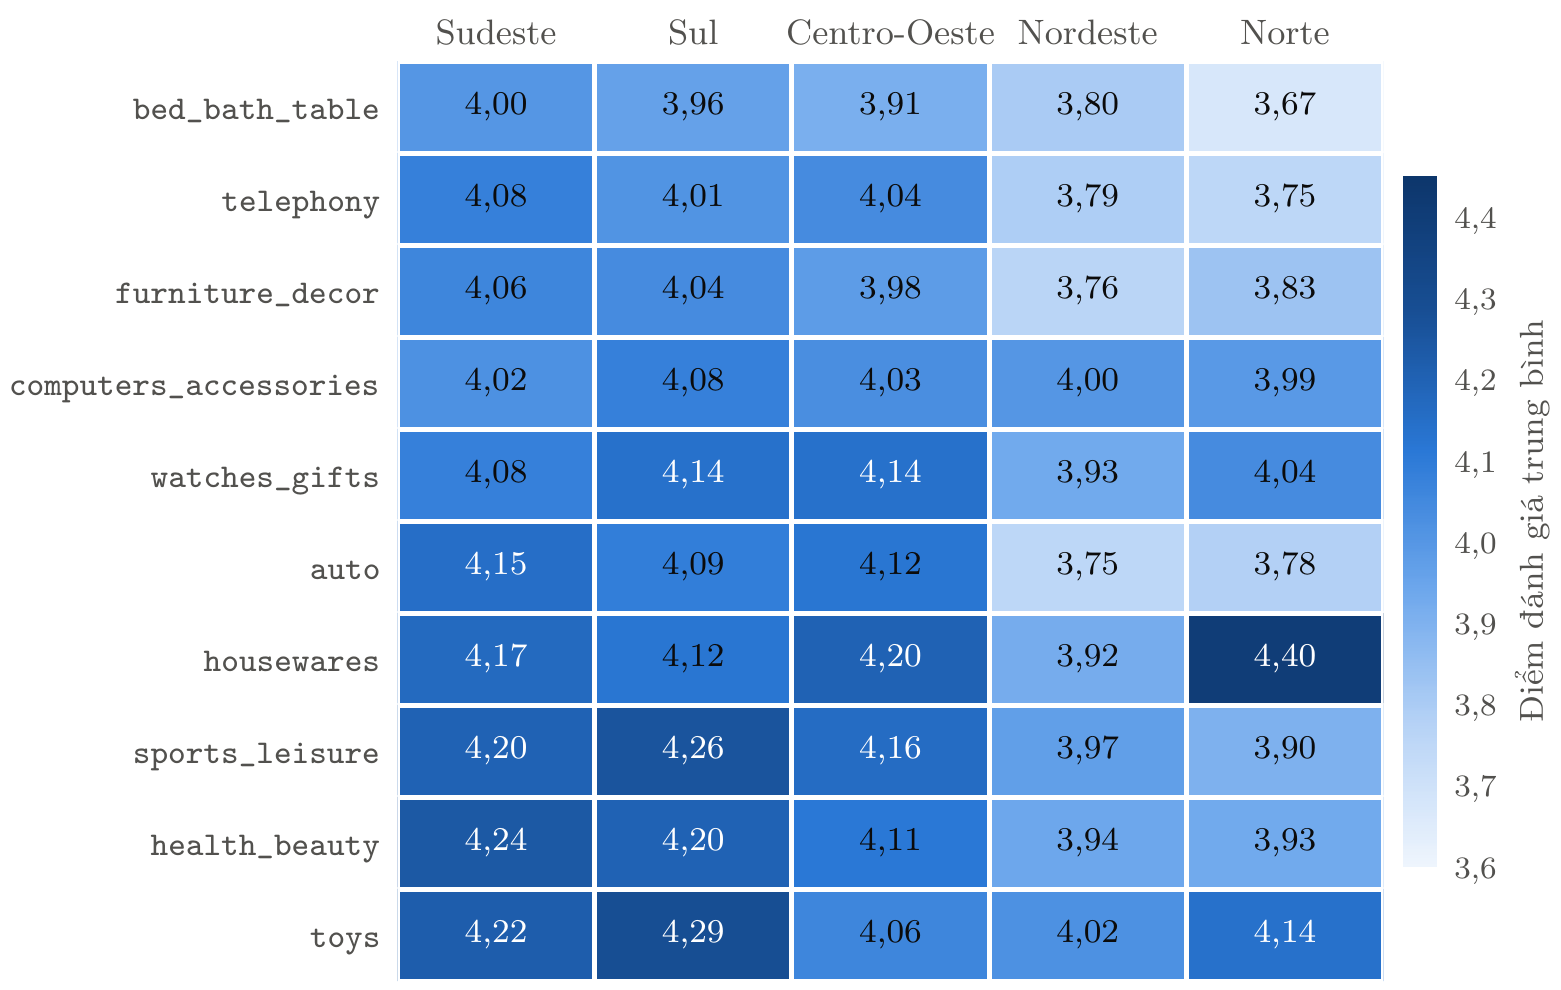
\includegraphics{Pictures/fig-olap-pivot.png}
\caption{Kết quả pivot: điểm đánh giá trung bình theo ngành hàng (dòng) và vùng của khách hàng (cột); màu càng đậm điểm càng cao}
\label{fig:pivot}
\end{figure}

Hai cột Nordeste và Norte nhạt hơn hẳn ba cột còn lại ở hầu hết các ngành hàng. Đây cũng là hai vùng có thời gian giao lâu nhất (Bảng~\ref{tab:drilldown}), một dấu hiệu nữa cho thấy điểm đánh giá gắn chặt với chất lượng giao hàng. Ô nổi bật duy nhất là \code{housewares} ở Norte (4,40), nhưng ô này chỉ dựa trên khoảng 60 đơn nên không đủ để kết luận.

\subsubsection{Các truy vấn phân tích nghiệp vụ}\label{sec:olapnghiepvu}

Ngoài năm phép toán cơ bản, thư viện truy vấn còn trả lời trực tiếp các câu hỏi của từng nhóm người dùng ở Bảng~\ref{tab:quyetdinh}.

\paragraph{Giao trễ và mức độ hài lòng}
Câu hỏi đầu tiên là giao trễ ảnh hưởng đến điểm đánh giá nhiều đến đâu. Trên 95.824 đơn có cả trạng thái giao hàng lẫn đánh giá, đơn đúng hạn được trung bình 4,29 điểm, còn đơn trễ chỉ 2,27 điểm. Hình~\ref{fig:trevadanhgia} cho thấy rõ hơn: hơn một nửa (53,8\%) đơn trễ bị chấm 1 sao, trong khi ở nhóm đúng hạn con số này chỉ là 6,6\%. Tỷ lệ 1-2 sao tăng từ 9,3\% lên 62,4\%. Với bộ phận chăm sóc khách hàng, điều này có nghĩa là giảm giao trễ là cách trực tiếp nhất để giảm đánh giá xấu; đây cũng là lý do thành phần hệ hỗ trợ quyết định của đề tài tập trung vào giao trễ.

\begin{figure}[H]
\centering
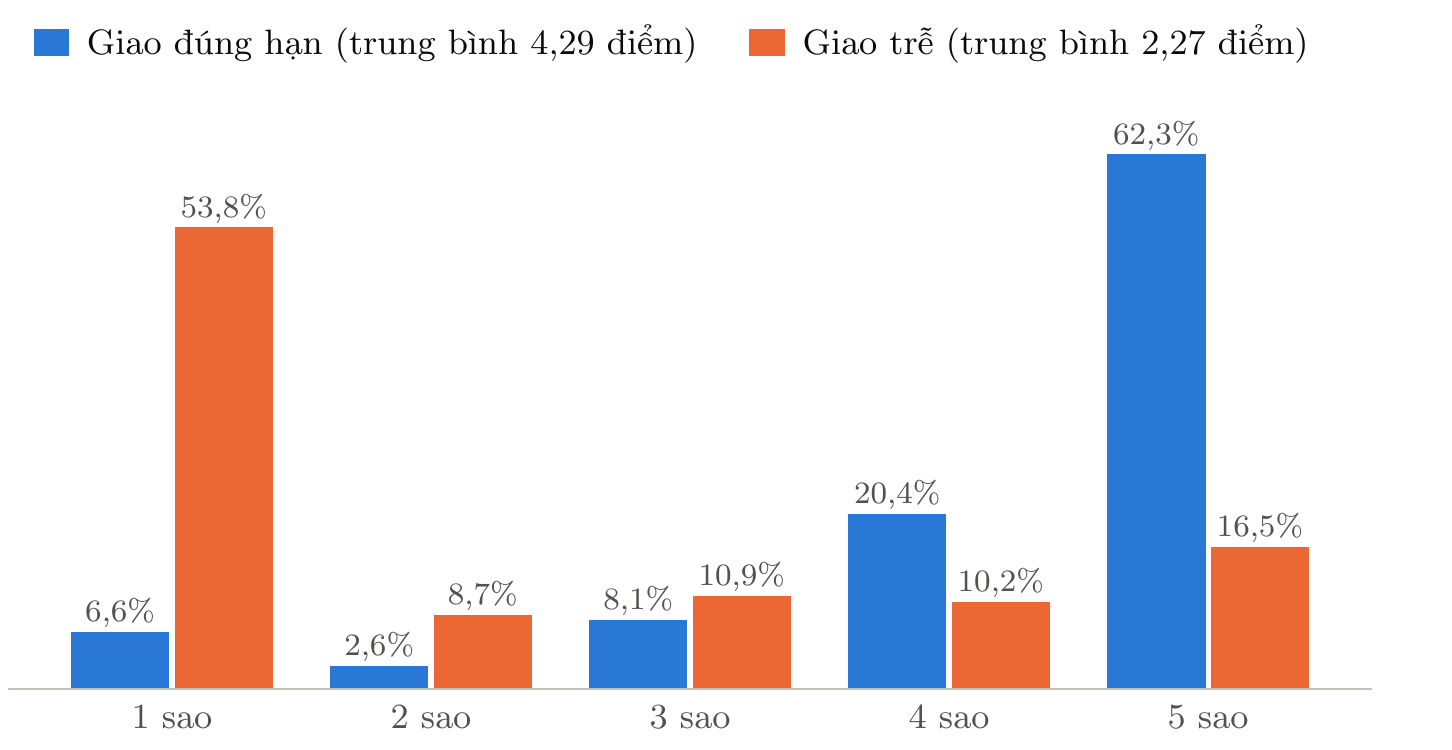
\includegraphics{Pictures/fig-tre-va-danh-gia.png}
\caption{Phân bố điểm đánh giá của đơn giao đúng hạn và đơn giao trễ}
\label{fig:trevadanhgia}
\end{figure}

\paragraph{Thời gian từng công đoạn}
Hình~\ref{fig:congdoan} tách thời gian giao hàng của mỗi vùng thành ba công đoạn. Thời gian duyệt đơn (0,41-0,52 ngày) và thời gian người bán chuẩn bị hàng (2,74-2,93 ngày) gần như giống nhau ở mọi vùng. Toàn bộ chênh lệch nằm ở khâu vận chuyển: 7,55 ngày tới Sudeste, nhưng 16,64 ngày tới Nordeste và 19,24 ngày tới Norte. Nói cách khác, khách ở miền Bắc nhận hàng chậm không phải do người bán chậm mà do quãng đường vận chuyển; muốn cải thiện thì phải làm việc với đơn vị vận chuyển hoặc phát triển người bán ngay tại các vùng này.

\begin{figure}[H]
\centering
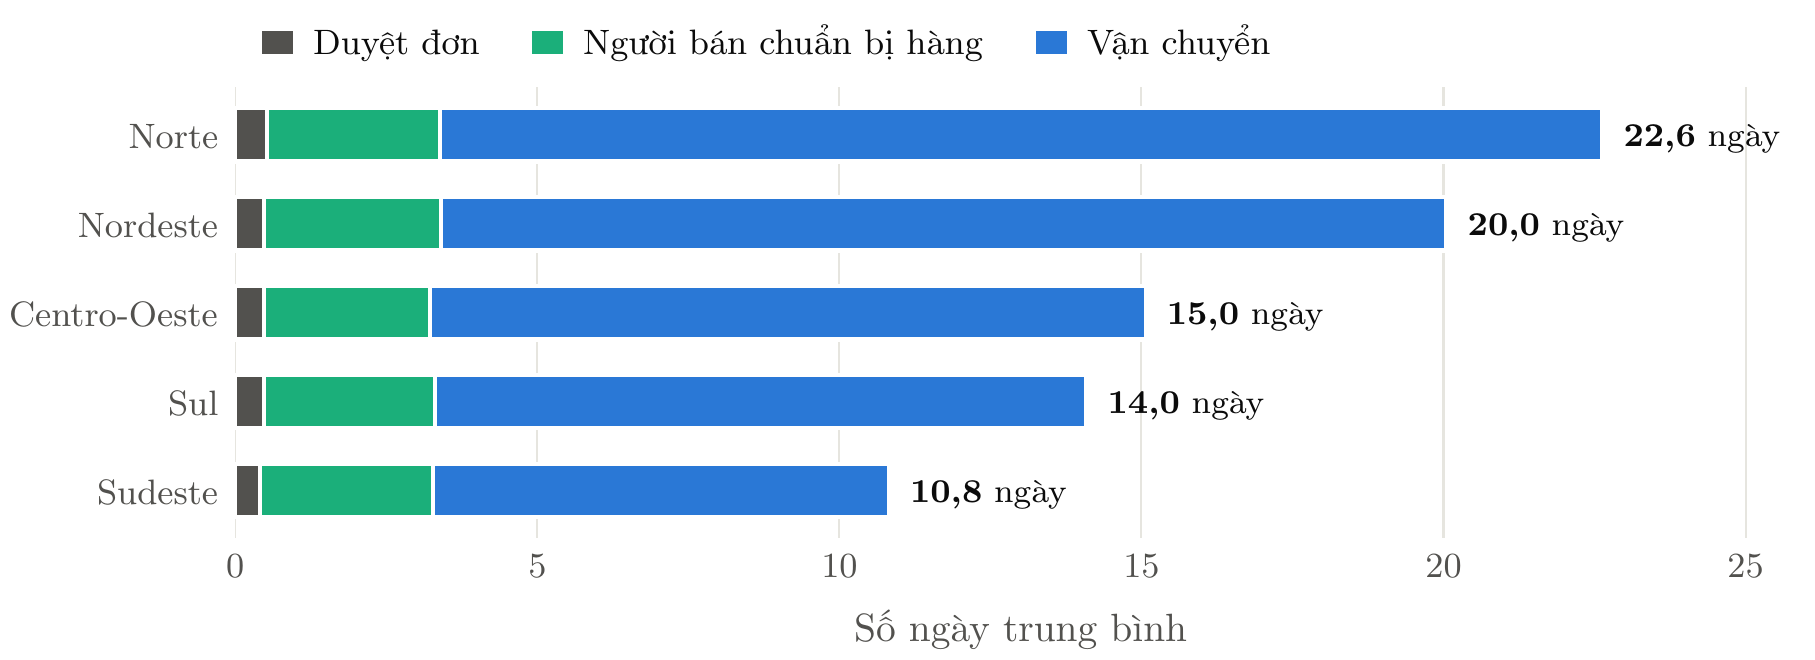
\includegraphics{Pictures/fig-olap-cong-doan.png}
\caption{Thời gian trung bình của từng công đoạn giao hàng theo vùng của khách hàng}
\label{fig:congdoan}
\end{figure}

\paragraph{Tuyến giao hàng}
Ma trận tuyến (Hình~\ref{fig:tuyengiao}) xét các lô hàng, tức cặp (đơn hàng, người bán), theo bang của người bán và bang của khách. Trong 50 tuyến có từ 200 lô trở lên, tỷ lệ trễ dao động từ 1,1\% (MG $\rightarrow$ PR) đến 23,7\% (SP $\rightarrow$ AL). Mọi tuyến từ SP đi các bang Nordeste đều trễ từ khoảng 10\% trở lên, cao nhất là đi AL, MA, PI và SE. Tuyến cần ưu tiên nhất với quản lý vận hành là SP $\rightarrow$ RJ: tỷ lệ trễ 14,0\% không phải cao nhất, nhưng tuyến này có tới 8.273 lô, nên đây là nơi cải thiện sẽ giảm được nhiều đơn trễ nhất.

\begin{figure}[H]
\centering
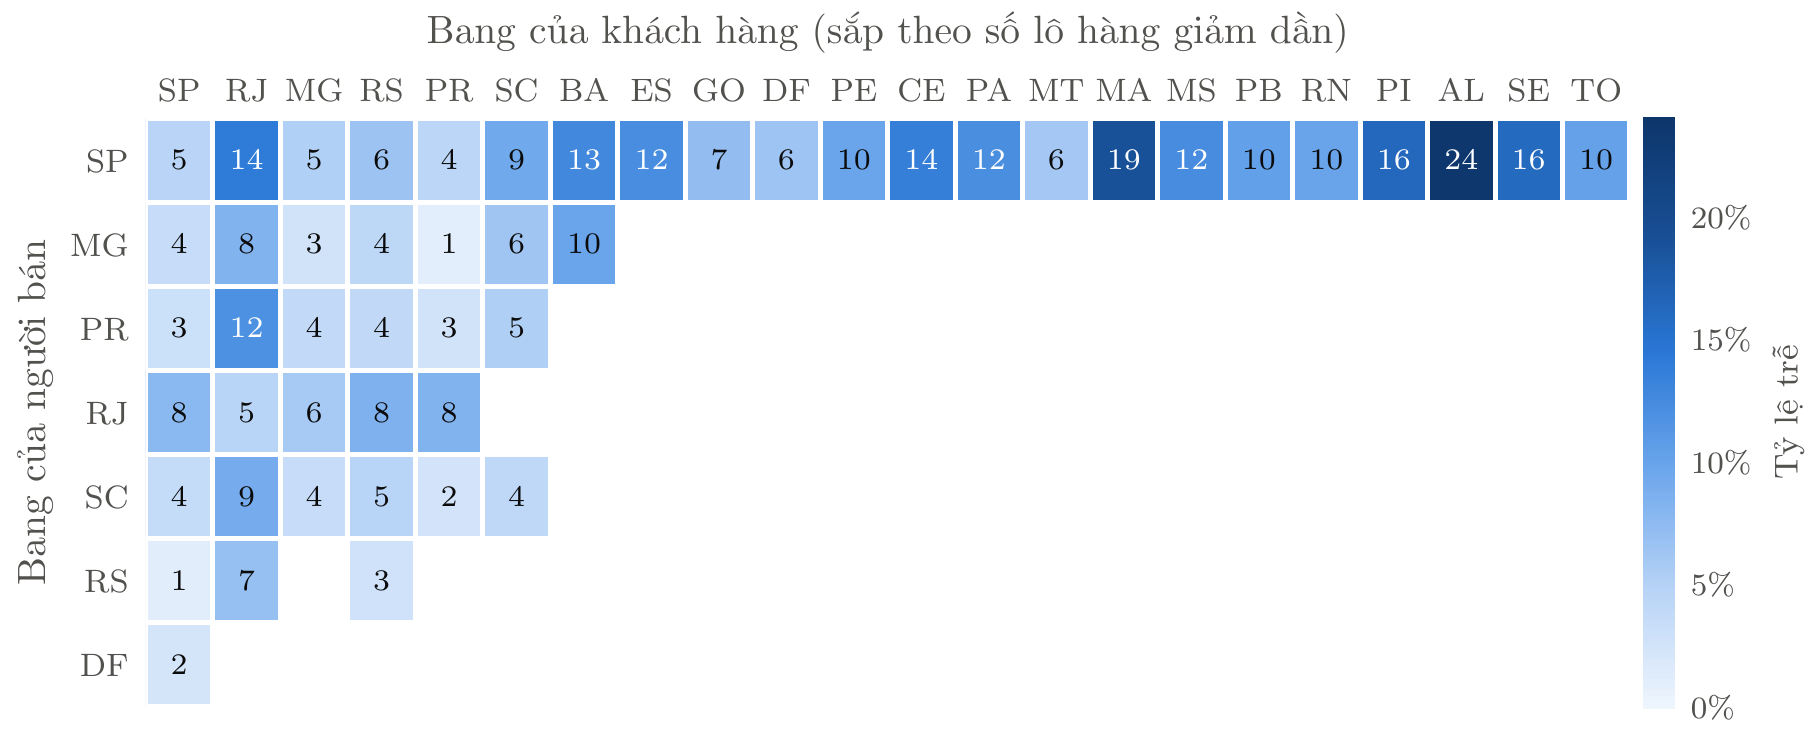
\includegraphics{Pictures/fig-olap-tuyen-giao.png}
\caption{Tỷ lệ giao trễ (\%) theo tuyến từ bang người bán đến bang khách hàng, chỉ gồm các tuyến có từ 200 lô hàng trở lên}
\label{fig:tuyengiao}
\end{figure}

\paragraph{Mùa cao điểm}
Ngày Black Friday 24/11/2017 có 1.166 đơn hàng, gấp hơn năm lần số đơn mỗi ngày của tuần trước đó (từ 146 đến 277 đơn). Hình~\ref{fig:blackfriday} cho thấy cái giá của đợt cao điểm này: các đơn đặt từ 24/11 đến 29/11/2017 có tỷ lệ trễ 17,3-20,9\%, gấp khoảng ba lần trung bình toàn kỳ, và phải sang tuần thứ hai của tháng 12 tỷ lệ trễ mới trở lại bình thường. Trước mùa cao điểm năm sau, sàn có cơ sở để nới ngày giao dự kiến hoặc tăng năng lực vận chuyển.

\begin{figure}[H]
\centering
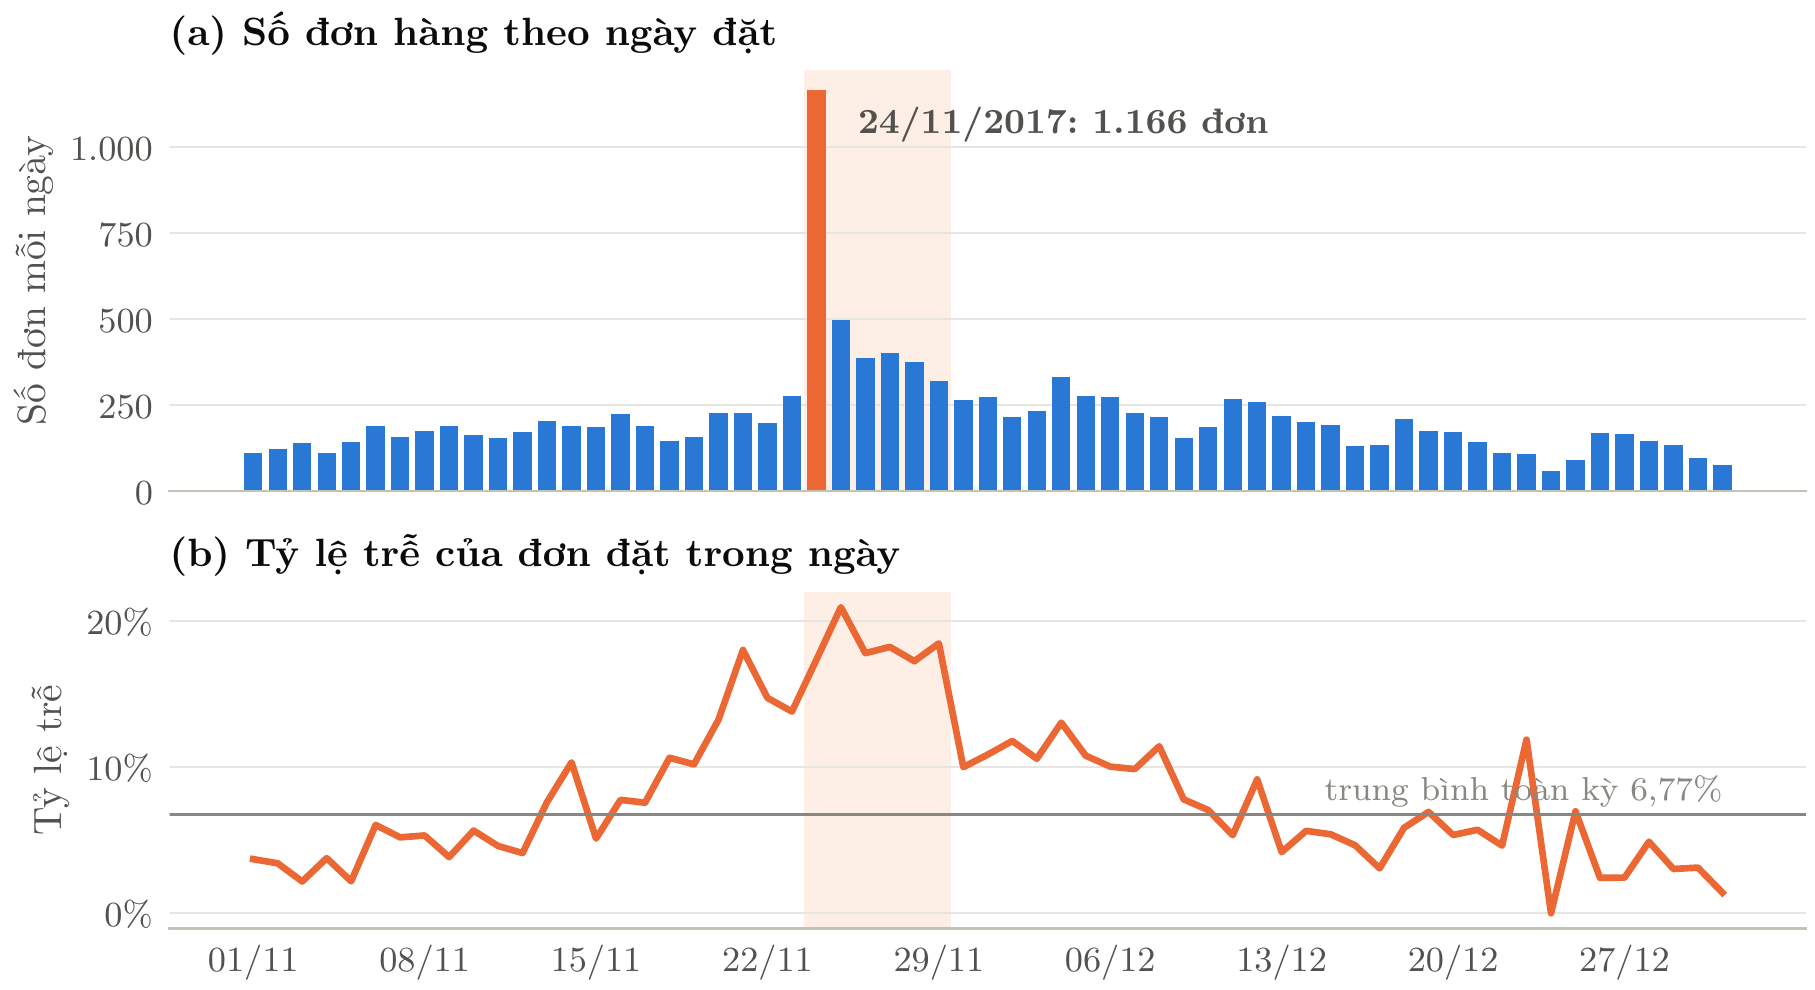
\includegraphics{Pictures/fig-olap-black-friday.png}
\caption{Số đơn hàng theo ngày (trên) và tỷ lệ giao trễ của đơn đặt trong ngày (dưới), tháng 11-12/2017; vùng tô xám là 24-29/11/2017}
\label{fig:blackfriday}
\end{figure}

\paragraph{Ngành hàng tăng trưởng}
So với cùng kỳ tháng 01-08/2017, doanh thu tháng 01-08/2018 của mọi ngành hàng lớn đều tăng, nhưng tốc độ rất khác nhau (Hình~\ref{fig:tangtruong}). \code{baby}, \code{watches\_gifts} và \code{health\_beauty} tăng hơn gấp ba, trong khi \code{cool\_stuff} gần như đứng yên (+8,9\%). Với ban điều hành, nhóm ngành tăng nhanh là ứng viên cho việc mở rộng danh mục người bán.

\begin{figure}[H]
\centering
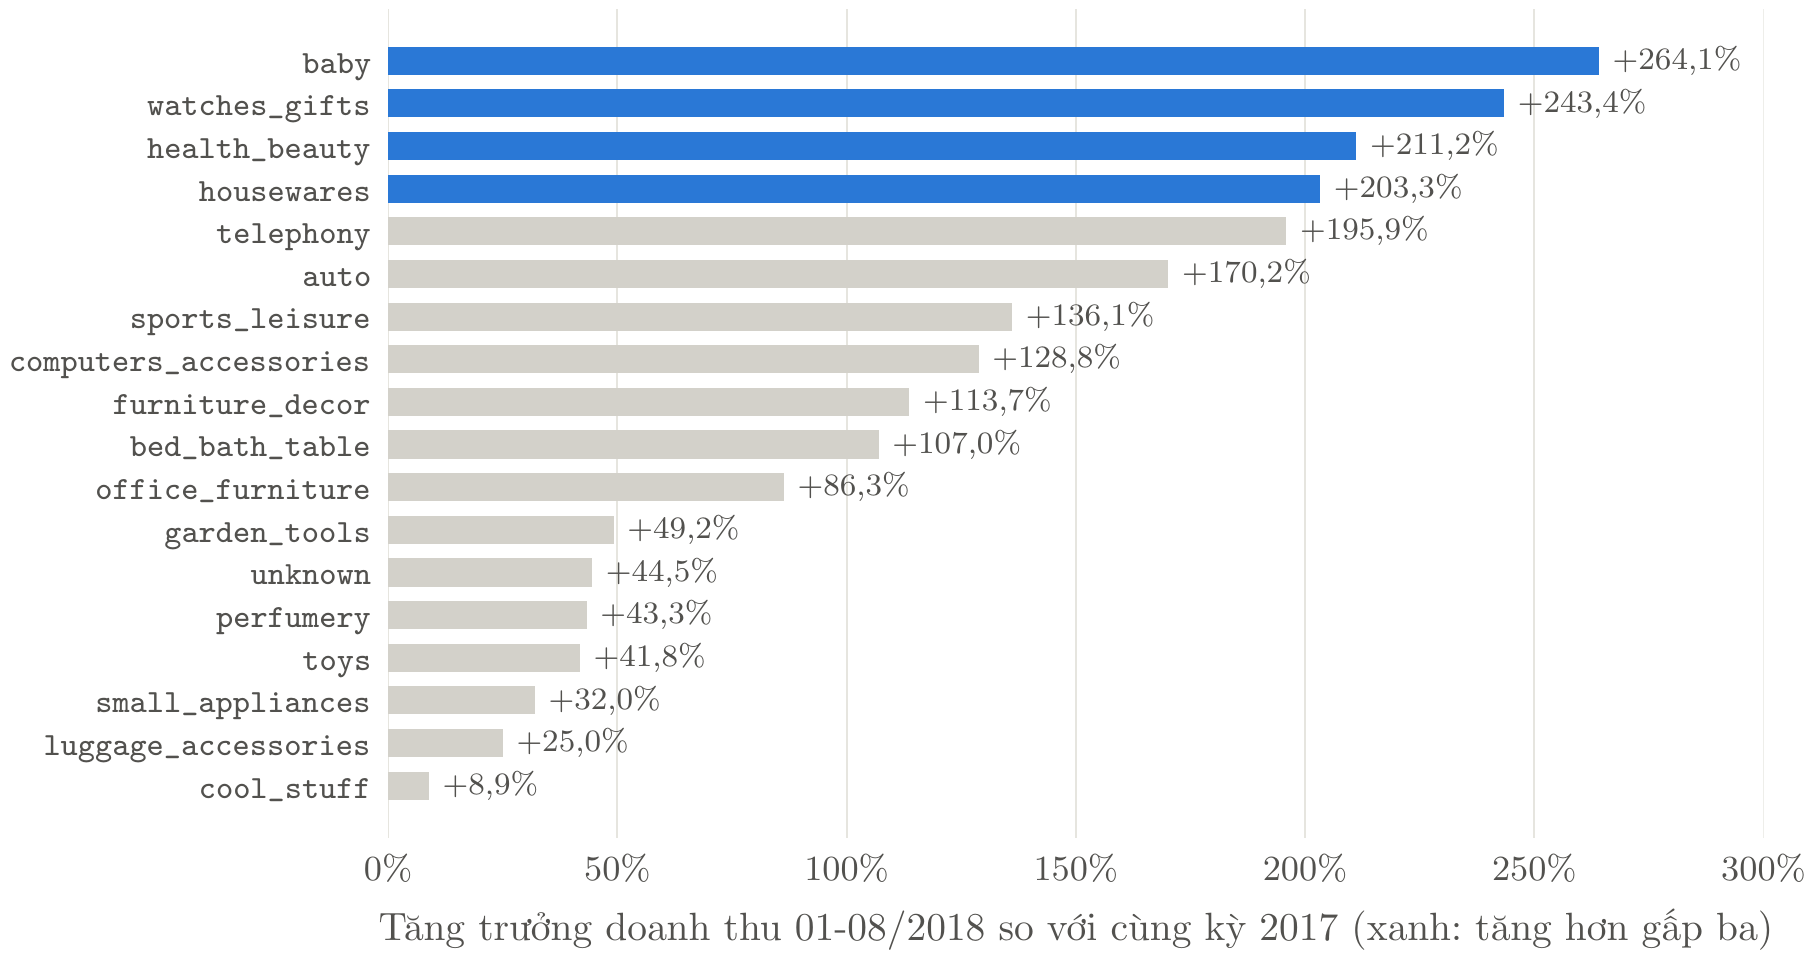
\includegraphics{Pictures/fig-olap-tang-truong-nganh.png}
\caption{Tăng trưởng doanh thu tháng 01-08/2018 so với cùng kỳ 2017 của các ngành hàng có doanh thu từ 50.000 BRL trong năm 2017}
\label{fig:tangtruong}
\end{figure}

\paragraph{Người bán}
Trong nhóm 20\% người bán có doanh thu cao nhất, có 12 người bán bị chấm 1-2 sao ở hơn một phần năm số đơn. Lớn nhất trong số này là một người bán có 973 đơn, doanh thu 186.570,05 BRL và 25,4\% đánh giá thấp. Đây là những người bán mà quản lý ngành hàng nên ưu tiên làm việc cùng, vì họ vừa đóng góp nhiều doanh thu vừa khiến không ít khách hàng không hài lòng. Ở góc độ phân bố, Hình~\ref{fig:nguoibankhachhang} cho thấy SP chiếm 59,7\% người bán nhưng chỉ 41,9\% đơn hàng, còn RJ có 12,9\% đơn hàng nhưng chỉ 5,5\% người bán. Phần lớn đơn của RJ vì vậy phải đi liên bang từ SP, và điều này khớp với tỷ lệ trễ cao của tuyến SP $\rightarrow$ RJ ở trên.

\begin{figure}[H]
\centering
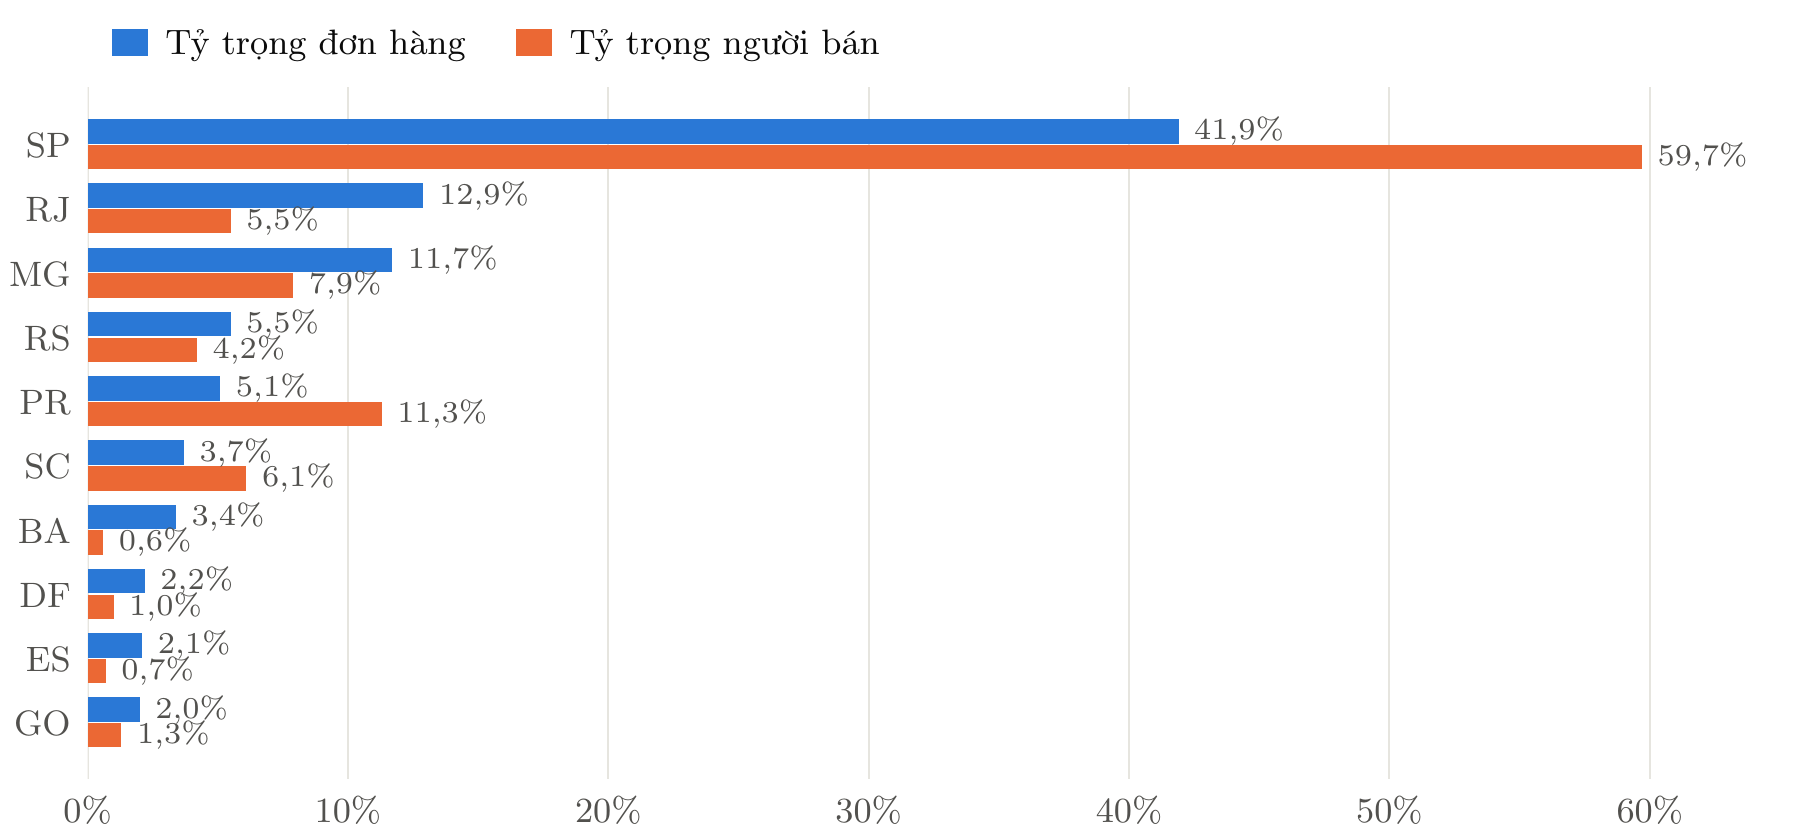
\includegraphics{Pictures/fig-olap-nguoi-ban-khach-hang.png}
\caption{Tỷ trọng người bán và tỷ trọng đơn hàng theo bang (10 bang có nhiều đơn hàng nhất)}
\label{fig:nguoibankhachhang}
\end{figure}

Đặt các kết quả này cạnh nhau sẽ ra một kết luận làm đầu vào cho phần hệ hỗ trợ quyết định: giao trễ là nguyên nhân chính làm giảm mức độ hài lòng, và giao trễ phụ thuộc rõ vào tuyến giao hàng, mùa vụ và người bán.

\subsubsection{Thời gian thực thi truy vấn}

Mỗi truy vấn được chạy năm lần bằng \code{EXPLAIN ANALYZE}, lấy trung vị thời gian thực thi trên máy chủ cơ sở dữ liệu (Bảng~\ref{tab:thoigiantruyvan}).

\begin{table}[H]
\centering
\small\setstretch{1.1}
\caption{Thời gian thực thi các truy vấn OLAP (trung vị của 5 lần chạy)}
\label{tab:thoigiantruyvan}
\begin{tabularx}{\linewidth}{|>{\raggedright\arraybackslash}X|P{2.0cm}|P{2.6cm}|}
\hline
\textbf{Truy vấn} & \textbf{Số dòng kết quả} & \textbf{Thời gian (ms)}\\ \hline
Roll-up doanh thu theo năm, quý, tháng & 37 & 545,6\\ \hline
Drill-down tỷ lệ trễ theo vùng, bang & 33 & 208,5\\ \hline
Drill-down tỷ lệ trễ theo thành phố của RJ & 4 & 100,3\\ \hline
Slice năm 2018 theo vùng & 5 & 219,0\\ \hline
Dice quý 4/2017 theo bang và ngành hàng & 15 & 230,1\\ \hline
Pivot điểm đánh giá theo ngành hàng và vùng & 10 & 454,9\\ \hline
Giao trễ và mức độ hài lòng & 2 & 74,6\\ \hline
Ma trận tuyến giao hàng & 50 & 311,8\\ \hline
Thời gian từng công đoạn theo vùng & 6 & 476,9\\ \hline
Người bán doanh thu cao, chất lượng thấp & 12 & 168,6\\ \hline
Phân bố người bán và đơn hàng theo bang & 27 & 179,8\\ \hline
Ngành hàng tăng trưởng & 18 & 57,7\\ \hline
CUBE vùng và năm & 24 & 717,3\\ \hline
Black Friday theo ngày & 15 & 93,5\\ \hline
\end{tabularx}
\end{table}

Truy vấn chậm nhất là CUBE theo vùng và năm, mất 0,72 giây, đủ nhanh để dashboard gọi trực tiếp. Kết quả này xác nhận nhận định ở mục~\ref{sec:luocdo}: với lượng dữ liệu hiện tại, các phép kết nối thêm của snowflake schema không làm chậm đáng kể, và chưa cần đến bảng tổng hợp lưu sẵn.

% !TeX root = ../../main.tex
\subsection{Dashboard và giao diện truy vấn}\label{sec:dashboard}

Dashboard được viết bằng Streamlit 1.67 và vẽ biểu đồ bằng Plotly 7.1. Nhóm chọn Streamlit vì ETL và DSS đều viết bằng Python, nên dashboard dùng chung môi trường và cấu hình kết nối mà không cần làm thêm frontend. Mỗi biểu đồ là một truy vấn SQL chạy trực tiếp trên Data Mart, đúng mô hình ROLAP ở mục~\ref{sec:kientruc}. Do Data Mart chỉ đổi sau mỗi lần chạy ETL, kết quả truy vấn được lưu đệm trong 10 phút. Mã nguồn nằm trong thư mục \code{src/dashboard}, gồm tập tin điều hướng \code{app.py}, phần kết nối \code{db.py}, bộ lọc \code{filters.py}, định dạng và màu biểu đồ \code{ui.py}, và mỗi trang một tập tin trong \code{views}.

Dashboard kết nối bằng tài khoản riêng \code{dashboard\_app}. Tài khoản này chỉ được đọc ba schema \code{dm}, \code{meta}, \code{dss} (quyền kế thừa từ role chỉ đọc \code{analyst\_ro}) và chỉ được thêm dòng vào bảng \code{dss.decision\_log}, nơi lưu các quyết định duyệt hay từ chối đề xuất của DSS. Nhóm đã thử sửa và xóa dòng trong bảng này bằng tài khoản trên, cả hai lệnh đều bị từ chối.

Để chạy dashboard, chỉ cần gõ \code{bash src/dashboard/run.sh} ở thư mục gốc. Kịch bản sẽ tự khởi động PostgreSQL, tạo môi trường Python, chạy ETL và chấm điểm DSS nếu chưa có dữ liệu, tạo tài khoản \code{dashboard\_app}, rồi mở dashboard tại \url{http://localhost:8501}; bước nào đã làm rồi thì bỏ qua.

\subsubsection{Tổ chức trang theo nhóm người dùng}

Các trang được nhóm theo người ra quyết định ở Bảng~\ref{tab:quyetdinh}, thêm một trang giám sát ETL cho người phụ trách kỹ thuật. Bảng~\ref{tab:dashboardtrang} liệt kê bảy trang cùng các truy vấn OLAP ở mục~\ref{sec:olap} mà mỗi trang dùng lại.

\begin{table}[H]
\centering
\small\setstretch{1.1}
\caption{Các trang của dashboard theo nhóm người dùng}
\label{tab:dashboardtrang}
\begin{tabularx}{\linewidth}{|P{3.0cm}|P{2.6cm}|>{\raggedright\arraybackslash}X|}
\hline
\textbf{Nhóm người dùng} & \textbf{Trang} & \textbf{Nội dung và phép OLAP}\\ \hline
Ban điều hành sàn & Tổng quan & Sáu chỉ số chính; doanh thu và số đơn theo tháng, quý hoặc năm (roll-up, drill-down); doanh thu theo vùng và năm (\code{CUBE})\\ \hline
Ban điều hành sàn & Doanh thu & Doanh thu theo vùng và 10 bang dẫn đầu; doanh thu ngành hàng $\times$ bang (dice); tăng trưởng ngành hàng 01-08/2018 so với cùng kỳ\\ \hline
Quản lý vận hành & Giao hàng & Tỷ lệ trễ drill-down vùng $\rightarrow$ bang $\rightarrow$ thành phố; thời gian từng công đoạn; ma trận tuyến giao hàng; mùa cao điểm Black Friday\\ \hline
Quản lý vận hành & Cảnh báo giao trễ & Phân tích what-if ngưỡng $p^{*}$, so sánh các chính sách; danh sách đơn ĐỎ, VÀNG theo ngày bàn giao kèm lý do; nút duyệt, từ chối\\ \hline
Chăm sóc khách hàng & Mức độ hài lòng & Phân bố điểm của đơn đúng hạn và đơn trễ; ngành hàng nhiều đánh giá 1-2 sao; pivot điểm theo ngành hàng và vùng, có nút hoán đổi trục\\ \hline
Quản lý ngành hàng và người bán & Người bán & Doanh thu và tỷ lệ đánh giá thấp của từng người bán; danh sách người bán cần làm việc trước với ngưỡng chỉnh được; phân bố người bán so với đơn hàng theo bang\\ \hline
Người phụ trách kỹ thuật & Giám sát ETL & Nhật ký từng bước, 20 tiêu chí đối soát, bản ghi bị loại hoặc bị sửa (schema \code{meta})\\ \hline
\end{tabularx}
\end{table}

\textbf{Bộ lọc.} Thanh bên trái có ba bộ lọc dùng chung cho các trang phân tích: khoảng tháng đặt hàng, vùng của khách hàng và ngành hàng. Về mặt OLAP, mỗi lần chọn bộ lọc là một phép slice hoặc dice trên khối dữ liệu. Giá trị đã chọn được giữ khi chuyển trang và được nhắc lại ngay dưới tên trang; nút ``Xóa bộ lọc'' đưa về toàn bộ dữ liệu.

\textbf{Truy vấn.} Mọi truy vấn của dashboard xuất phát từ hai biểu thức \code{WITH} dùng chung:
\begin{itemize}
    \item \code{items} đọc \code{fact\_sales}, dùng cho các thước đo cộng được như doanh thu, phí vận chuyển;
    \item \code{orders} đọc view \code{dm.v\_order}, dùng cho các thước đo theo đơn như thời gian giao, cờ trễ, điểm đánh giá.
\end{itemize}
Nhờ vậy dashboard giữ đúng quy ước ở mục~\ref{sec:dodo}: một đơn có nhiều sản phẩm vẫn chỉ được tính một lần.

\textbf{Hiển thị.} Dưới mỗi biểu đồ có mục ``Bảng số liệu'' để xem con số cụ thể. Mọi con số đều theo định dạng Việt Nam (13.494.400,74; 6,77\%). Người xem có thể chọn giao diện sáng hoặc tối, màu biểu đồ đổi theo.

\subsubsection{Các trang phân tích}

Trang Tổng quan (Hình~\ref{fig:dashtongquan}) là trang mặc định. Sáu ô chỉ số ở đầu trang trả lời ngay câu hỏi ``sàn đang bán được bao nhiêu và giao hàng thế nào''. Nút ``Tháng / Quý / Năm'' đổi mức tổng hợp của biểu đồ doanh thu, tức là roll-up hoặc drill-down trên phân cấp thời gian mà không phải viết lại truy vấn.

\begin{figure}[H]
\centering
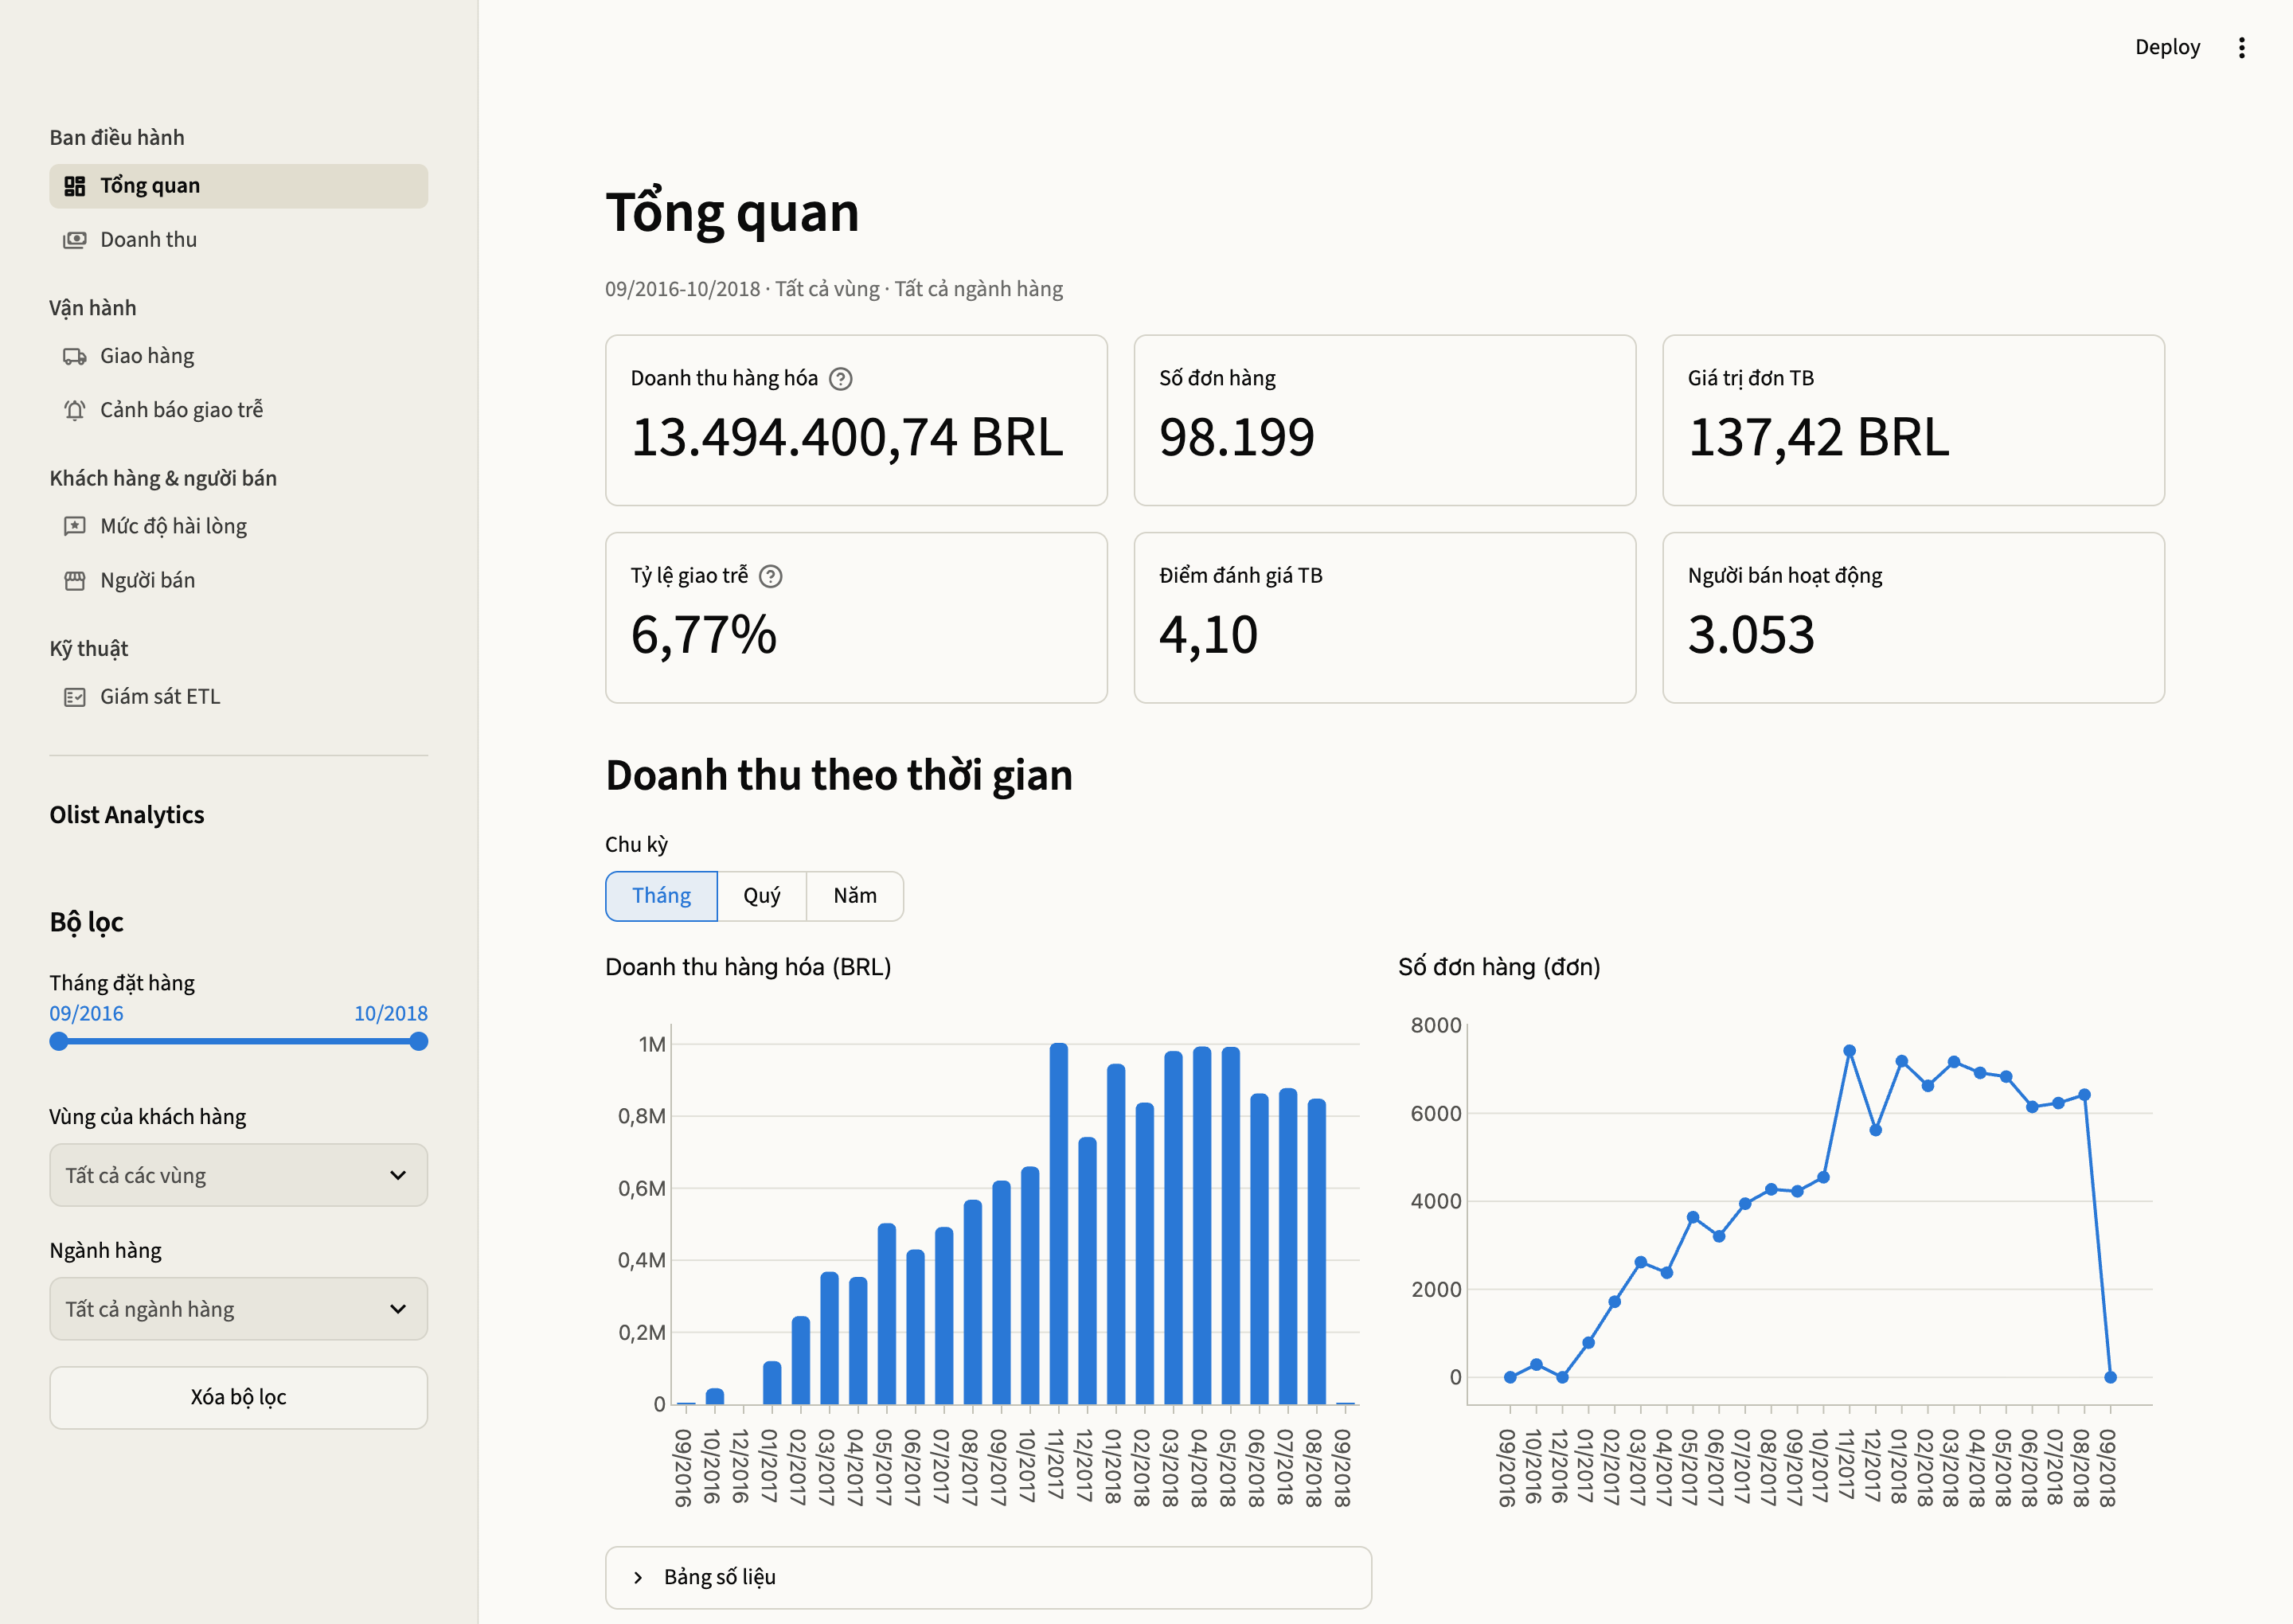
\includegraphics[width=\linewidth]{Pictures/dash-tong-quan.png}
\caption{Trang Tổng quan: thanh điều hướng và bộ lọc bên trái, sáu chỉ số chính và doanh thu theo tháng}
\label{fig:dashtongquan}
\end{figure}

Trang Doanh thu (Hình~\ref{fig:dashdoanhthu}) cho ban điều hành so sánh các thị trường. Biểu đồ nhiệt ngành hàng $\times$ bang là phép dice ở mục~\ref{sec:olap}, nhưng ở đây người xem tự chọn số ngành hàng; khi đổi bộ lọc thời gian sang năm 2018, biểu đồ theo vùng cho đúng kết quả slice ở Bảng~\ref{tab:slice}.

\begin{figure}[H]
\centering
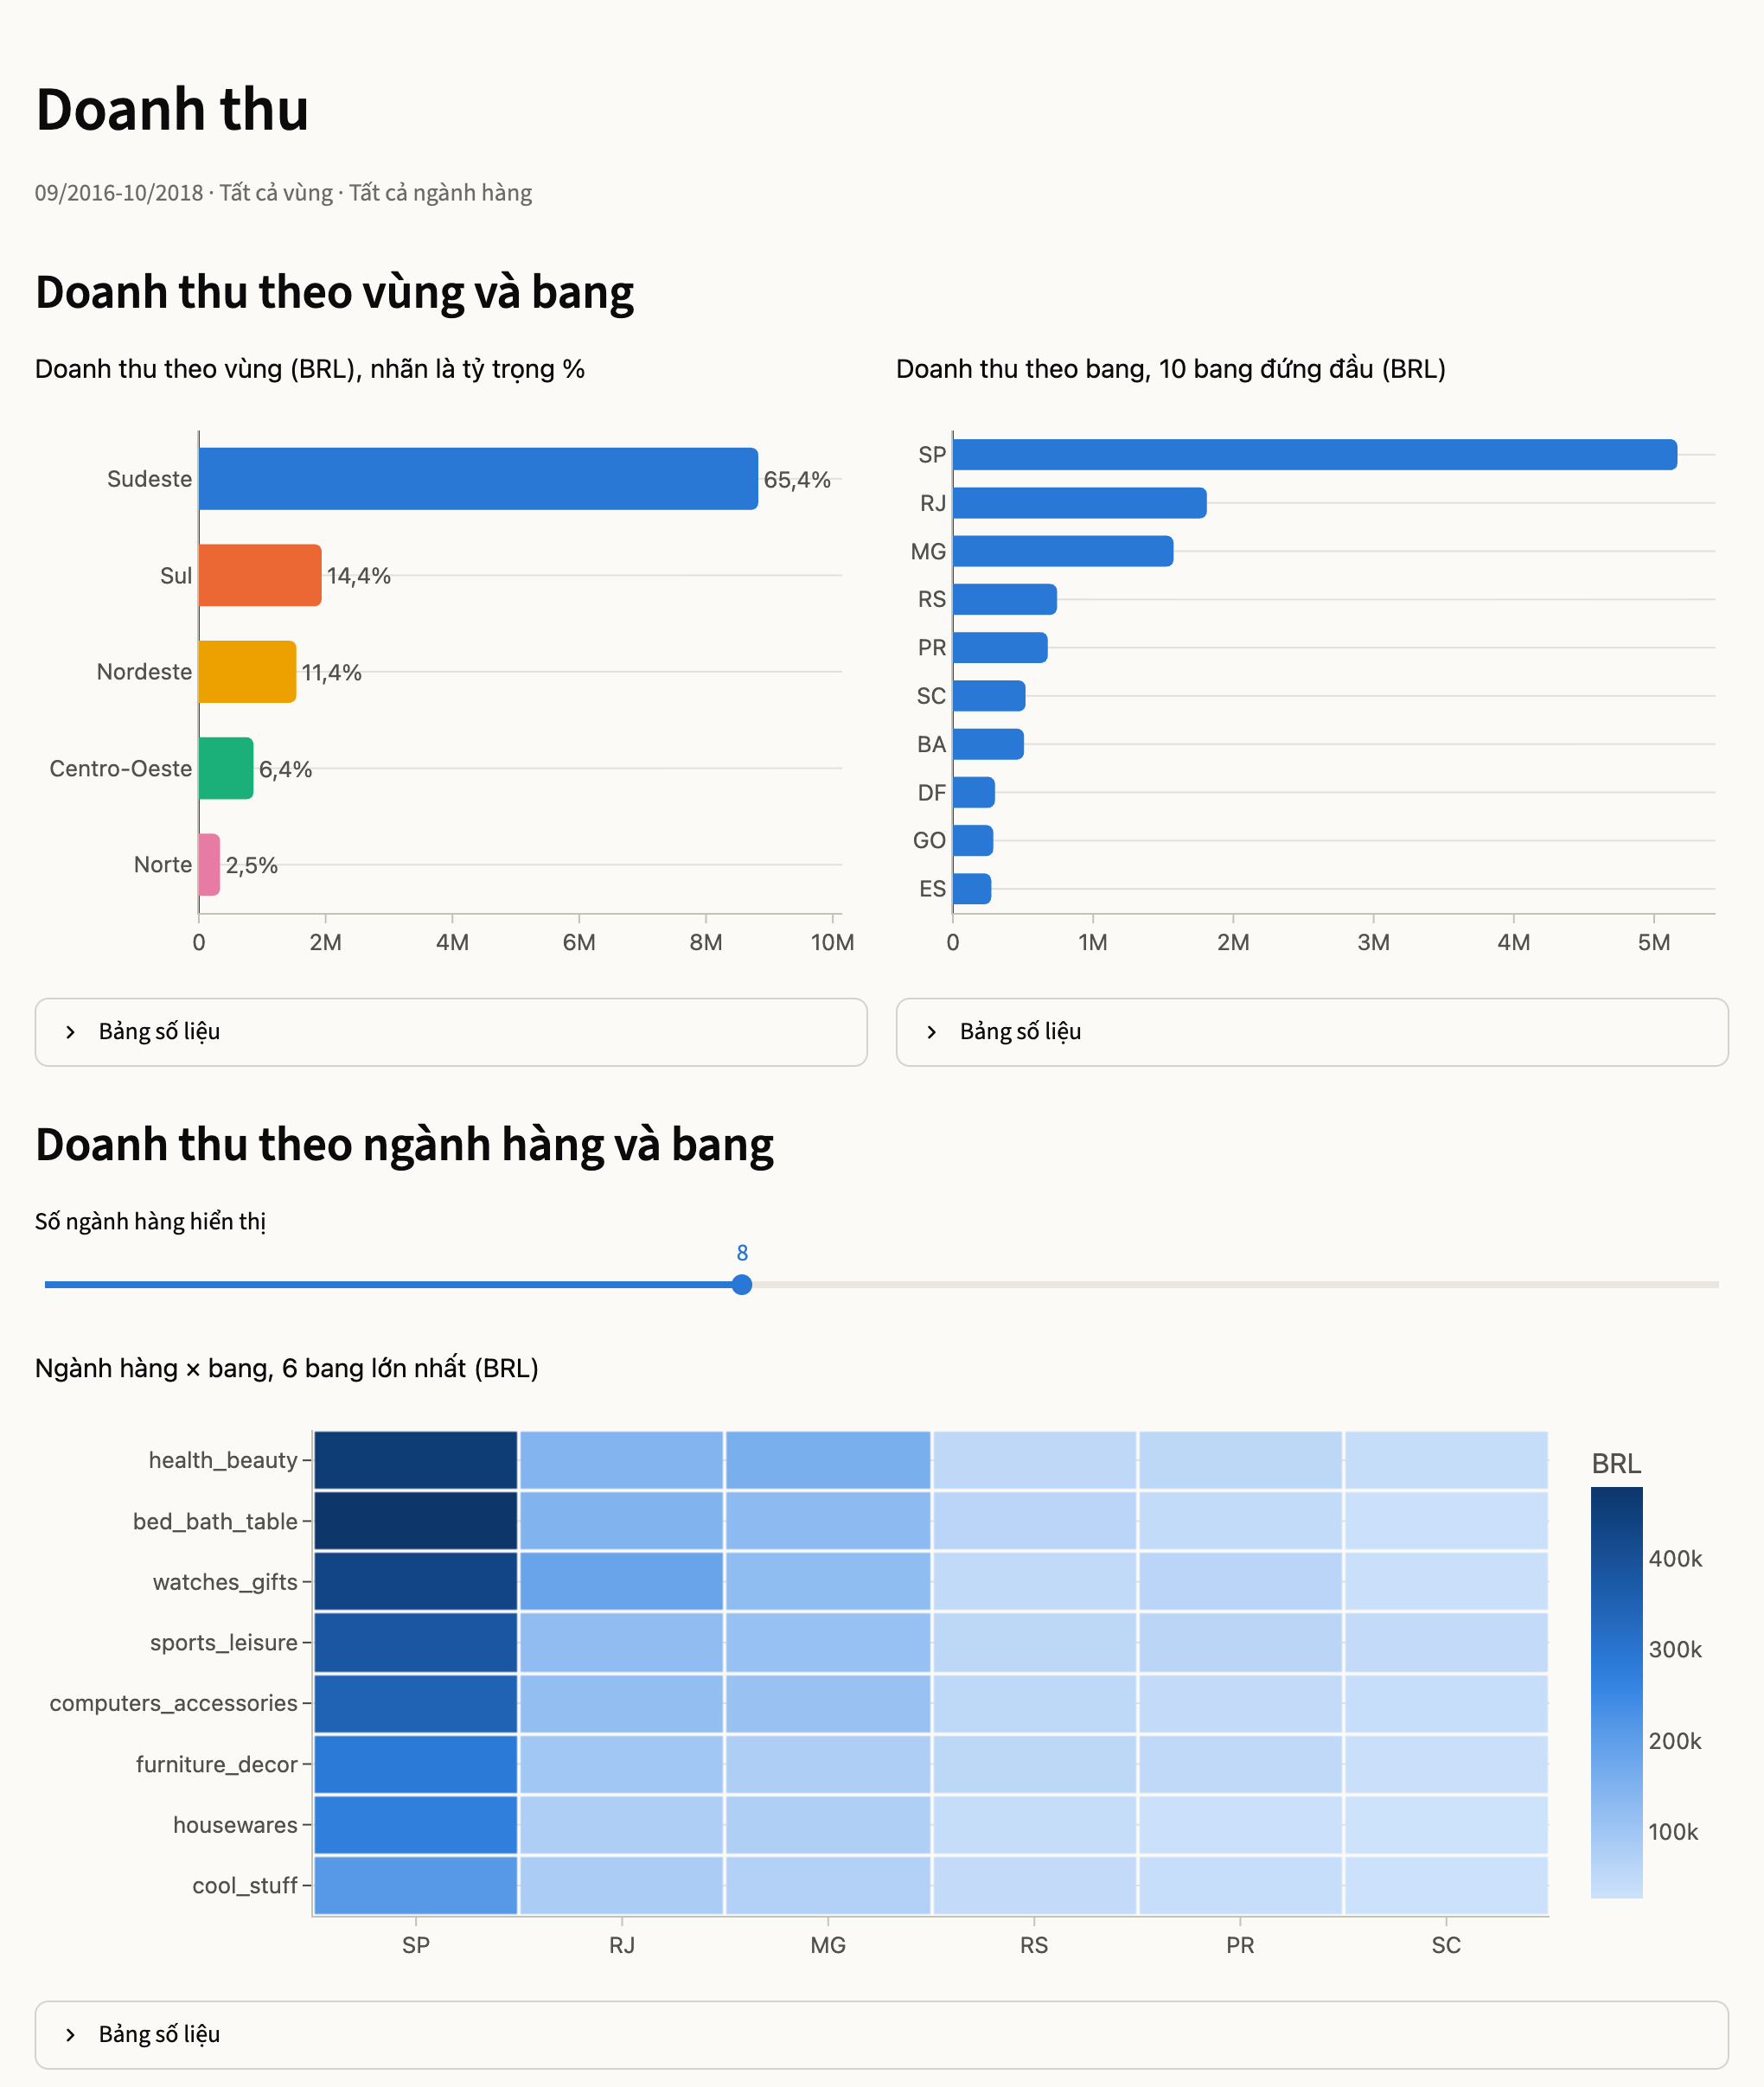
\includegraphics[width=\linewidth,height=0.55\textheight,keepaspectratio]{Pictures/dash-doanh-thu.png}
\caption{Trang Doanh thu: doanh thu theo vùng, theo bang và biểu đồ nhiệt ngành hàng $\times$ bang}
\label{fig:dashdoanhthu}
\end{figure}

Trang Giao hàng (Hình~\ref{fig:dashgiaohang}) dành cho quản lý vận hành. Hai ô chọn ``Vùng'' và ``Bang'' thực hiện drill-down từ toàn quốc xuống bang rồi xuống thành phố. Đường gạch ngang trên biểu đồ là tỷ lệ trễ toàn quốc, giúp nhận ra ngay các bang vượt trung bình. Phía dưới trang (không có trên hình) là thời gian từng công đoạn, ma trận tuyến giao hàng và biểu đồ mùa cao điểm; với ma trận tuyến, người xem chỉnh được số lô tối thiểu của một tuyến, vì tuyến quá ít lô cho tỷ lệ trễ không đáng tin.

\begin{figure}[H]
\centering
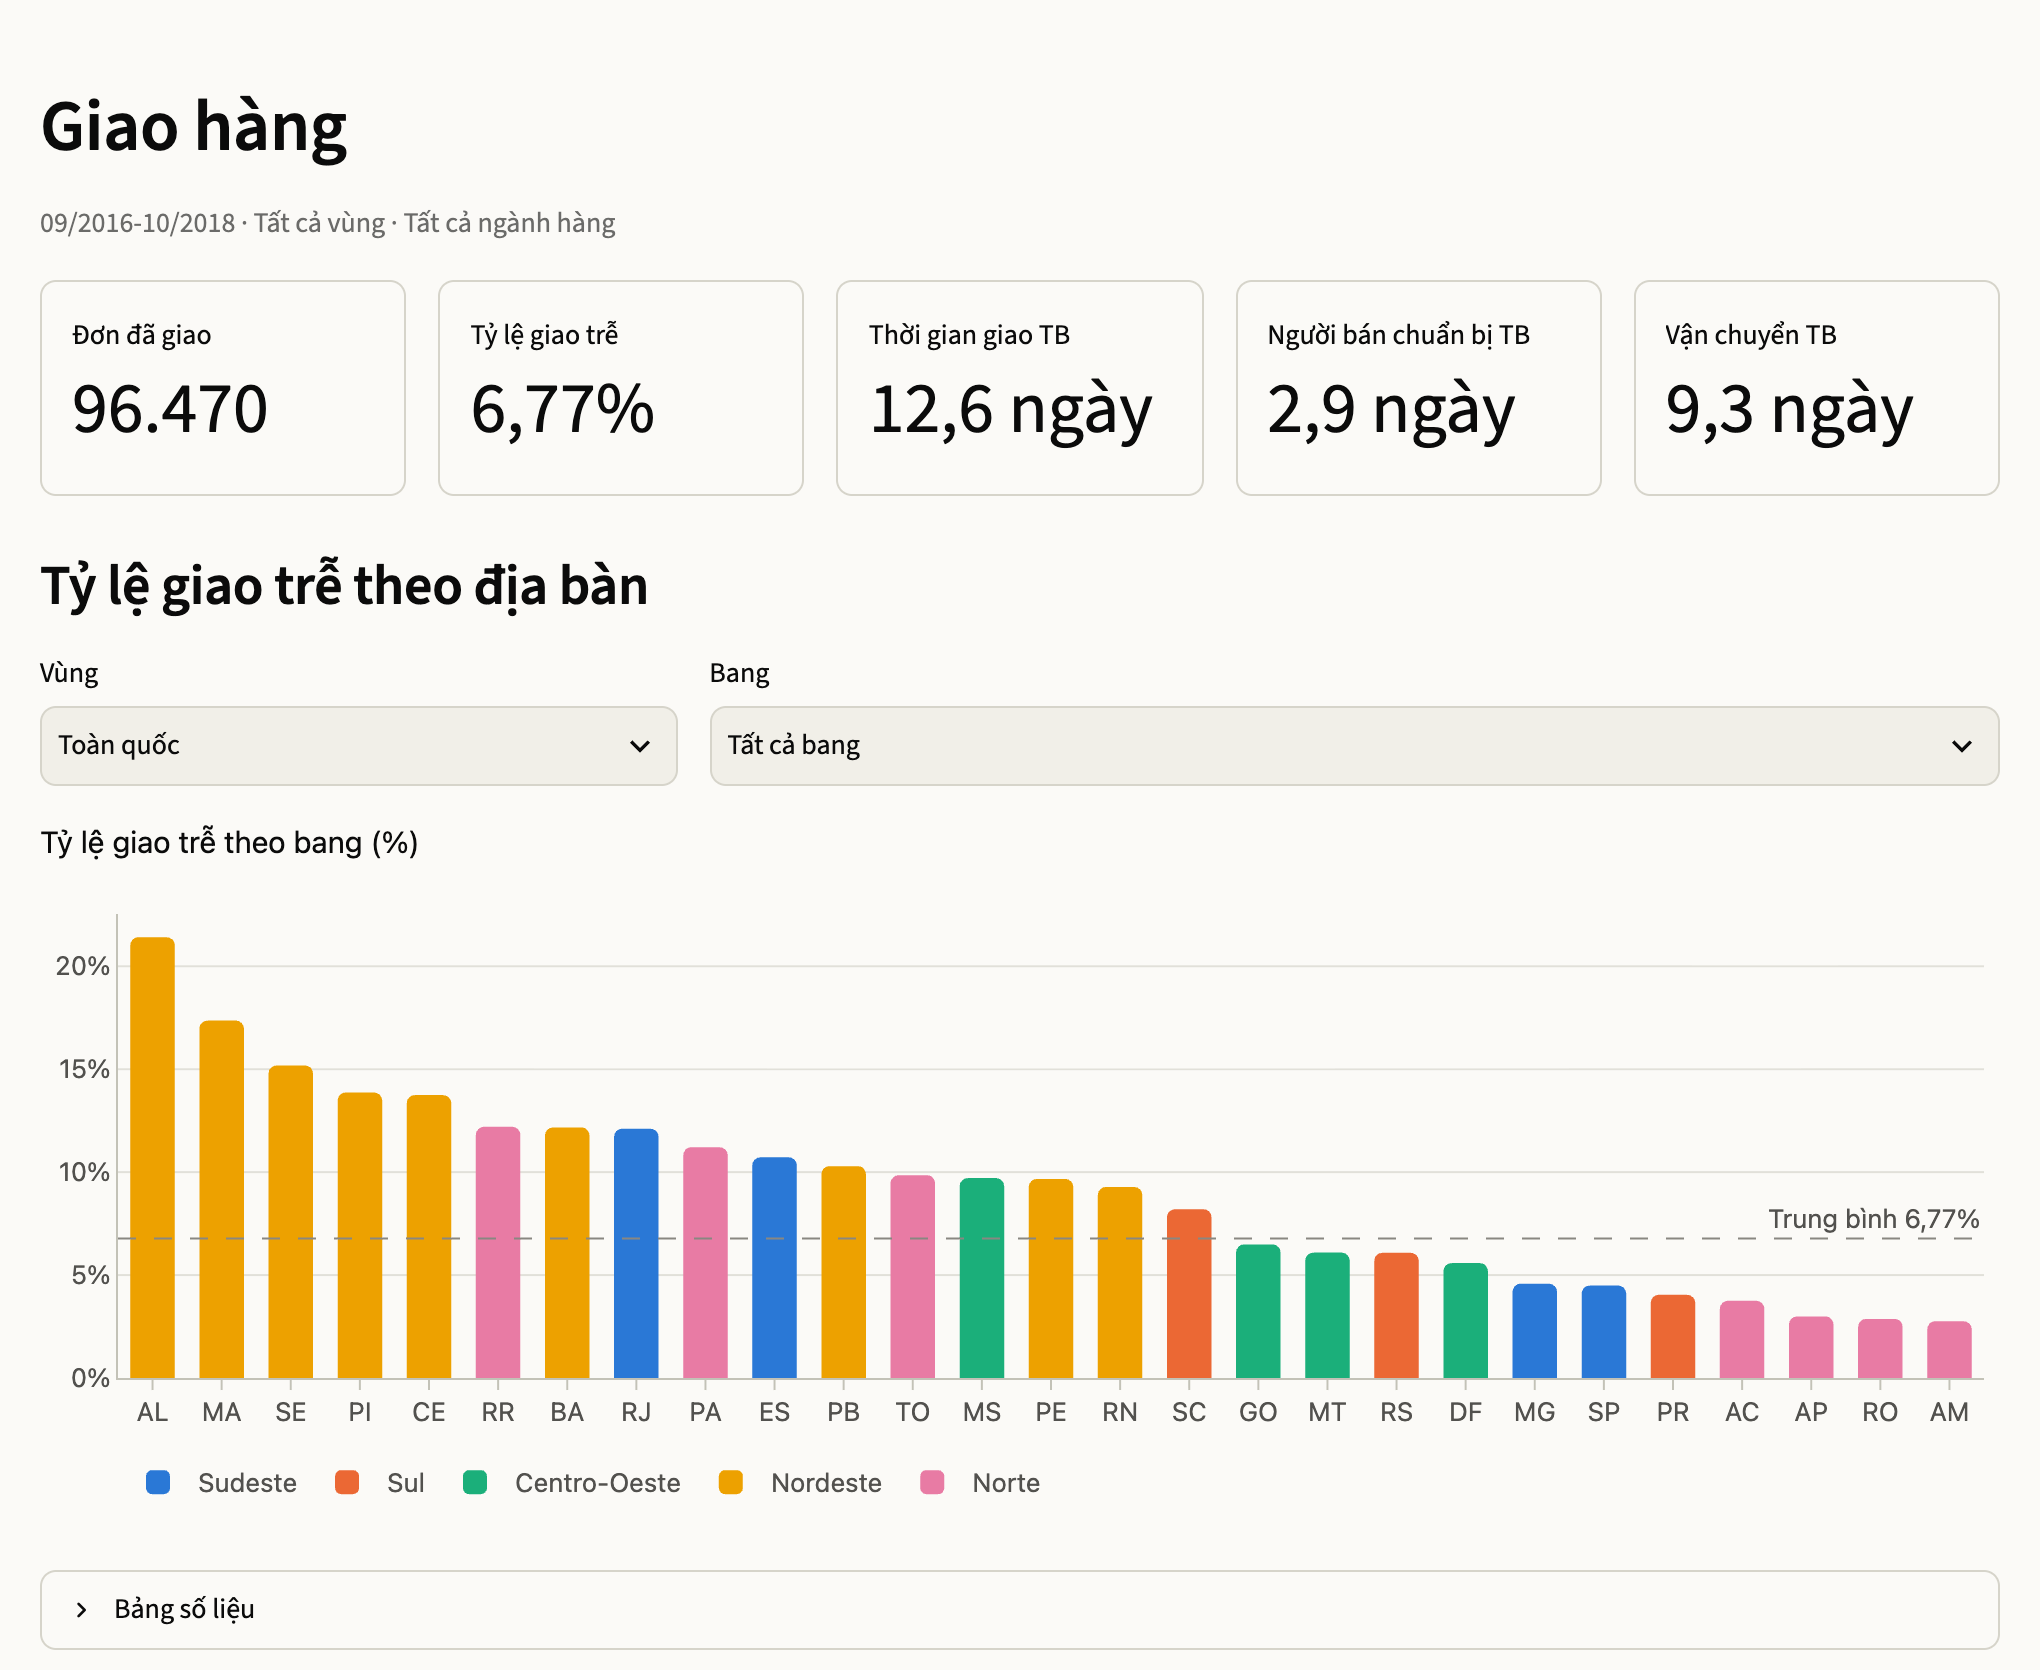
\includegraphics[width=\linewidth]{Pictures/dash-giao-hang.png}
\caption{Trang Giao hàng: chỉ số giao hàng và drill-down tỷ lệ trễ ở mức bang, tô màu theo vùng}
\label{fig:dashgiaohang}
\end{figure}

Trang Mức độ hài lòng (Hình~\ref{fig:dashhailong}) đặt cạnh nhau điểm đánh giá của đơn đúng hạn và đơn trễ, cùng danh sách ngành hàng có tỷ lệ 1-2 sao cao nhất. Phía dưới trang là phép pivot ngành hàng $\times$ vùng như Hình~\ref{fig:pivot}, kèm nút hoán đổi trục.

\begin{figure}[H]
\centering
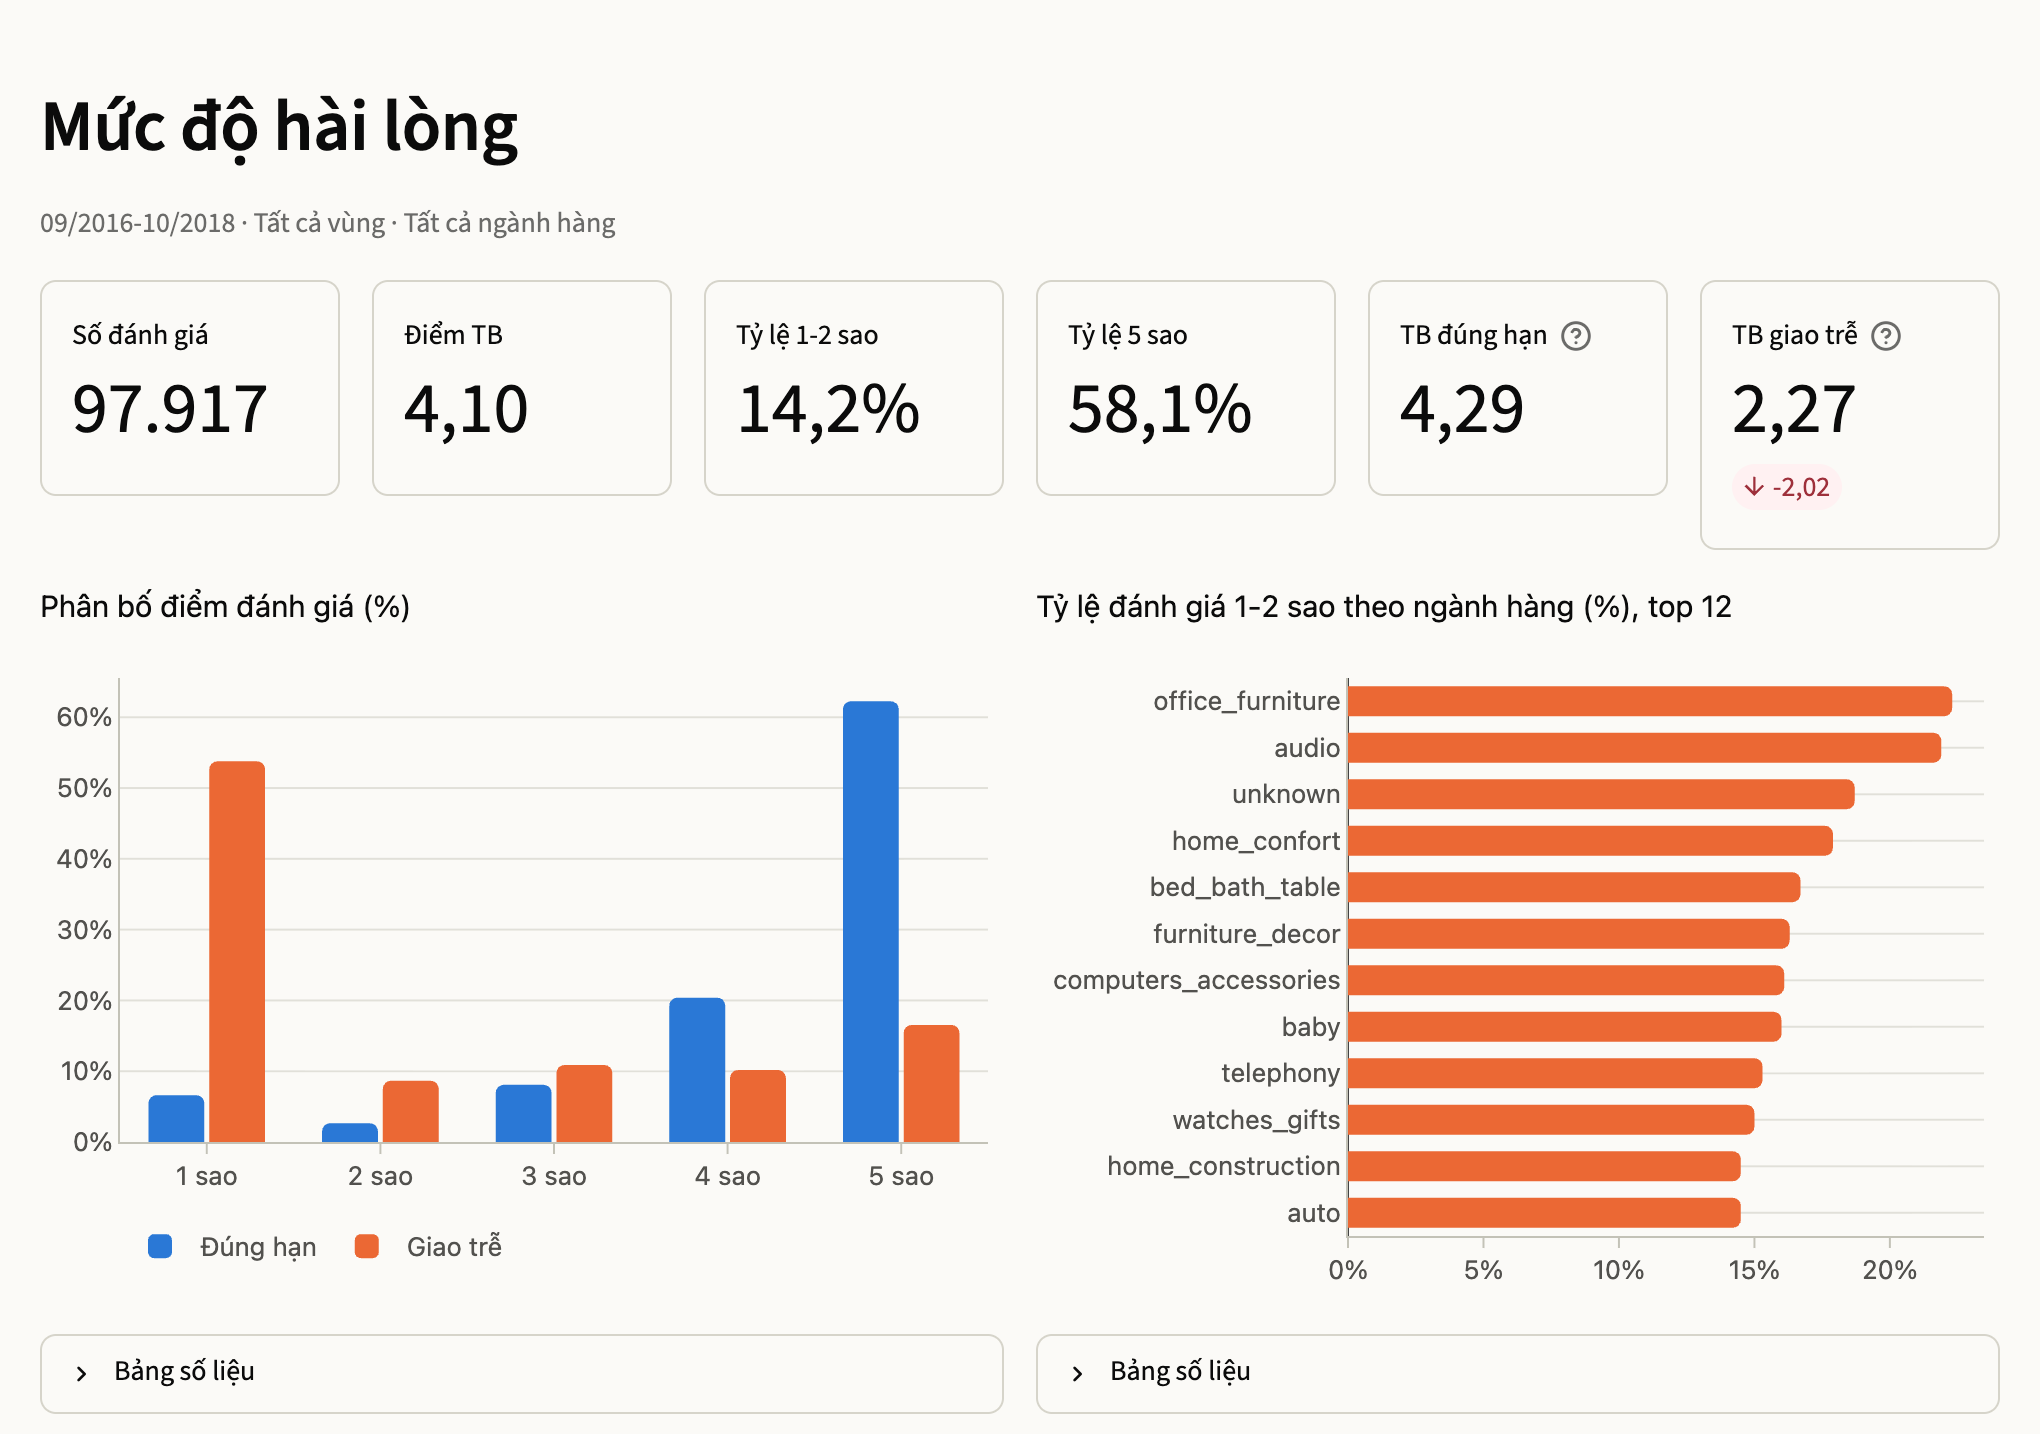
\includegraphics[width=\linewidth]{Pictures/dash-hai-long.png}
\caption{Trang Mức độ hài lòng: chỉ số đánh giá, phân bố điểm của đơn đúng hạn và đơn trễ, ngành hàng nhiều đánh giá thấp}
\label{fig:dashhailong}
\end{figure}

Trang Người bán (Hình~\ref{fig:dashnguoiban}) vẽ mỗi người bán thành một điểm theo doanh thu và tỷ lệ đánh giá 1-2 sao. Truy vấn ở mục~\ref{sec:olapnghiepvu} cố định hai ngưỡng ``20\% doanh thu cao nhất'' và ``hơn 20\% đánh giá thấp''; trên dashboard, quản lý ngành hàng chỉnh được cả hai ngưỡng và số đơn tối thiểu. Với giá trị mặc định, ô ``Cần xem xét'' cho đúng 12 người bán như truy vấn OLAP; bảng chi tiết ngay dưới biểu đồ xếp người bán có 973 đơn và 186.570,05 BRL doanh thu lên đầu. Các điểm màu cam trên biểu đồ là nhóm người bán này.

\begin{figure}[H]
\centering
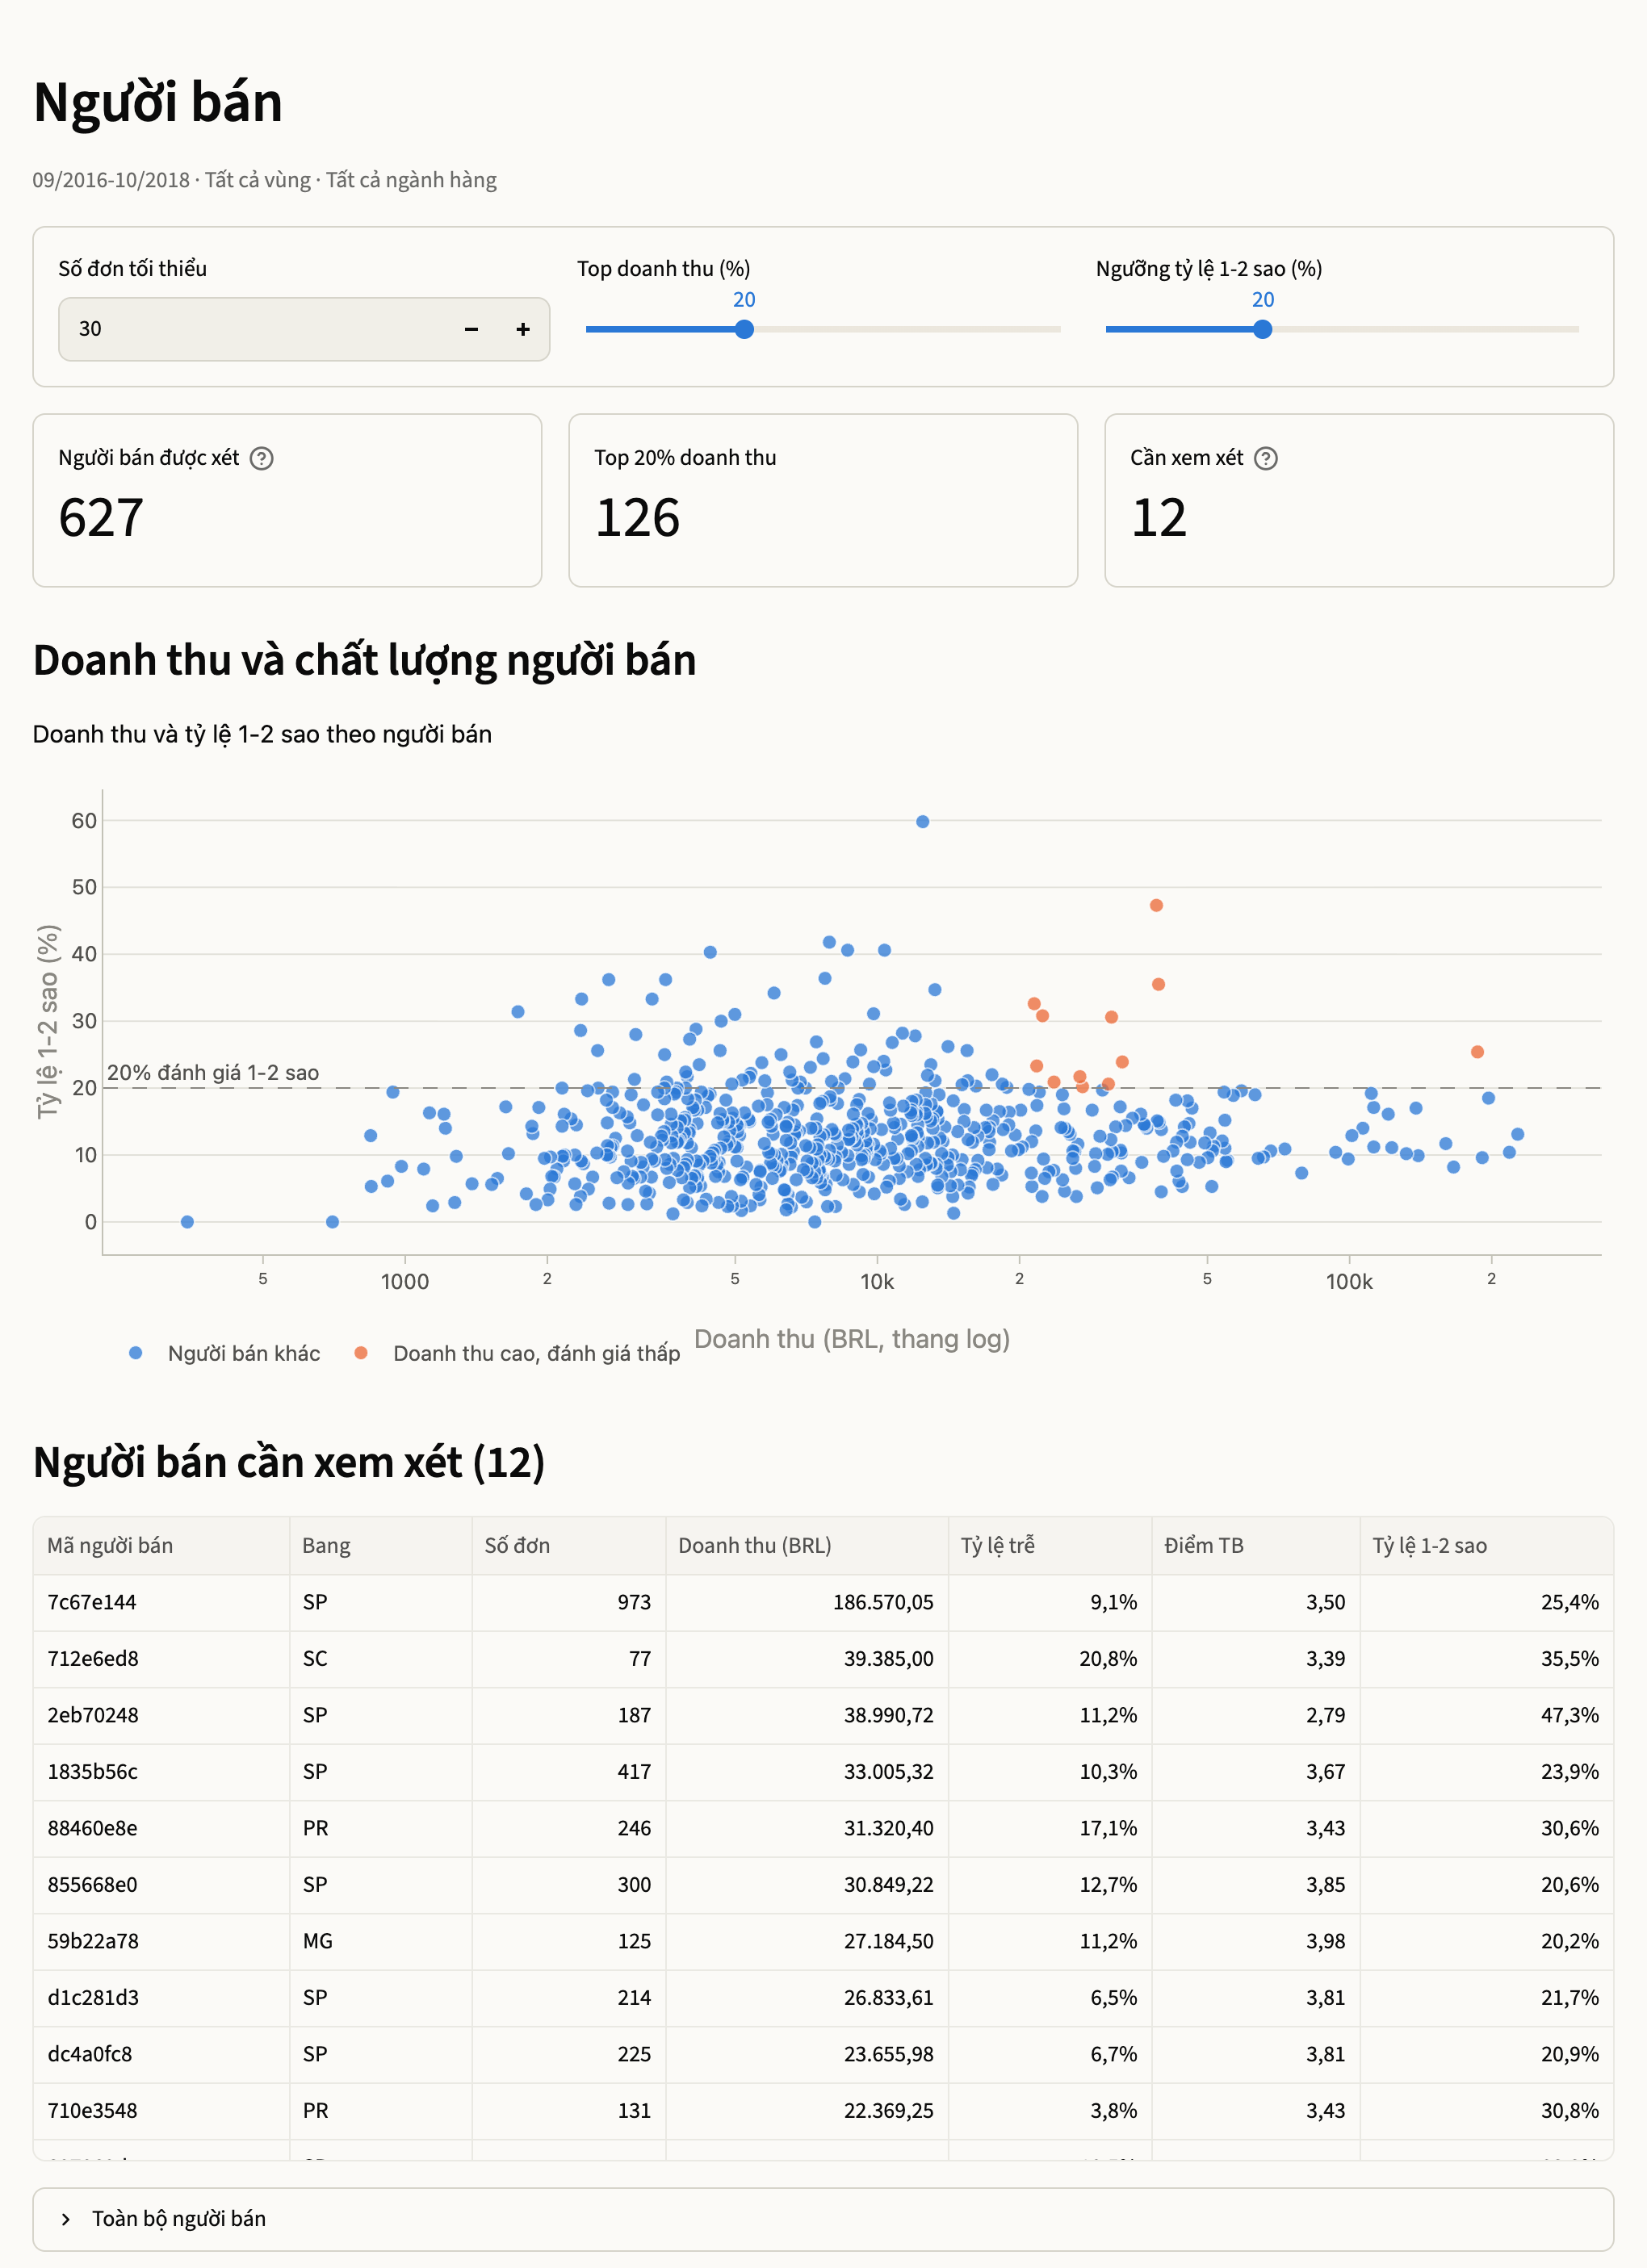
\includegraphics[width=\linewidth]{Pictures/dash-nguoi-ban.png}
\caption{Trang Người bán: ngưỡng chỉnh được, số người bán cần xem xét và biểu đồ phân tán doanh thu, tỷ lệ đánh giá 1-2 sao}
\label{fig:dashnguoiban}
\end{figure}

Trang Giám sát ETL (Hình~\ref{fig:dashetl}) đọc schema \code{meta}. Dòng trạng thái ở đầu trang cho biết ngay lần chạy có thành công hay không; bên dưới là trạng thái và số dòng của từng bước, kết quả 20 tiêu chí đối soát và các bản ghi bị loại hoặc bị sửa kèm lý do. Đây là chức năng giám sát (Monitoring) trong kiến trúc ở Hình~\ref{fig:kientruc}. Hình này hiện đúng lần chạy ETL ở Bảng~\ref{tab:etlbuoc}: 8,7 giây, 775 đơn bị loại, 1.458 bản ghi được sửa và 20/20 tiêu chí đạt.

\begin{figure}[H]
\centering
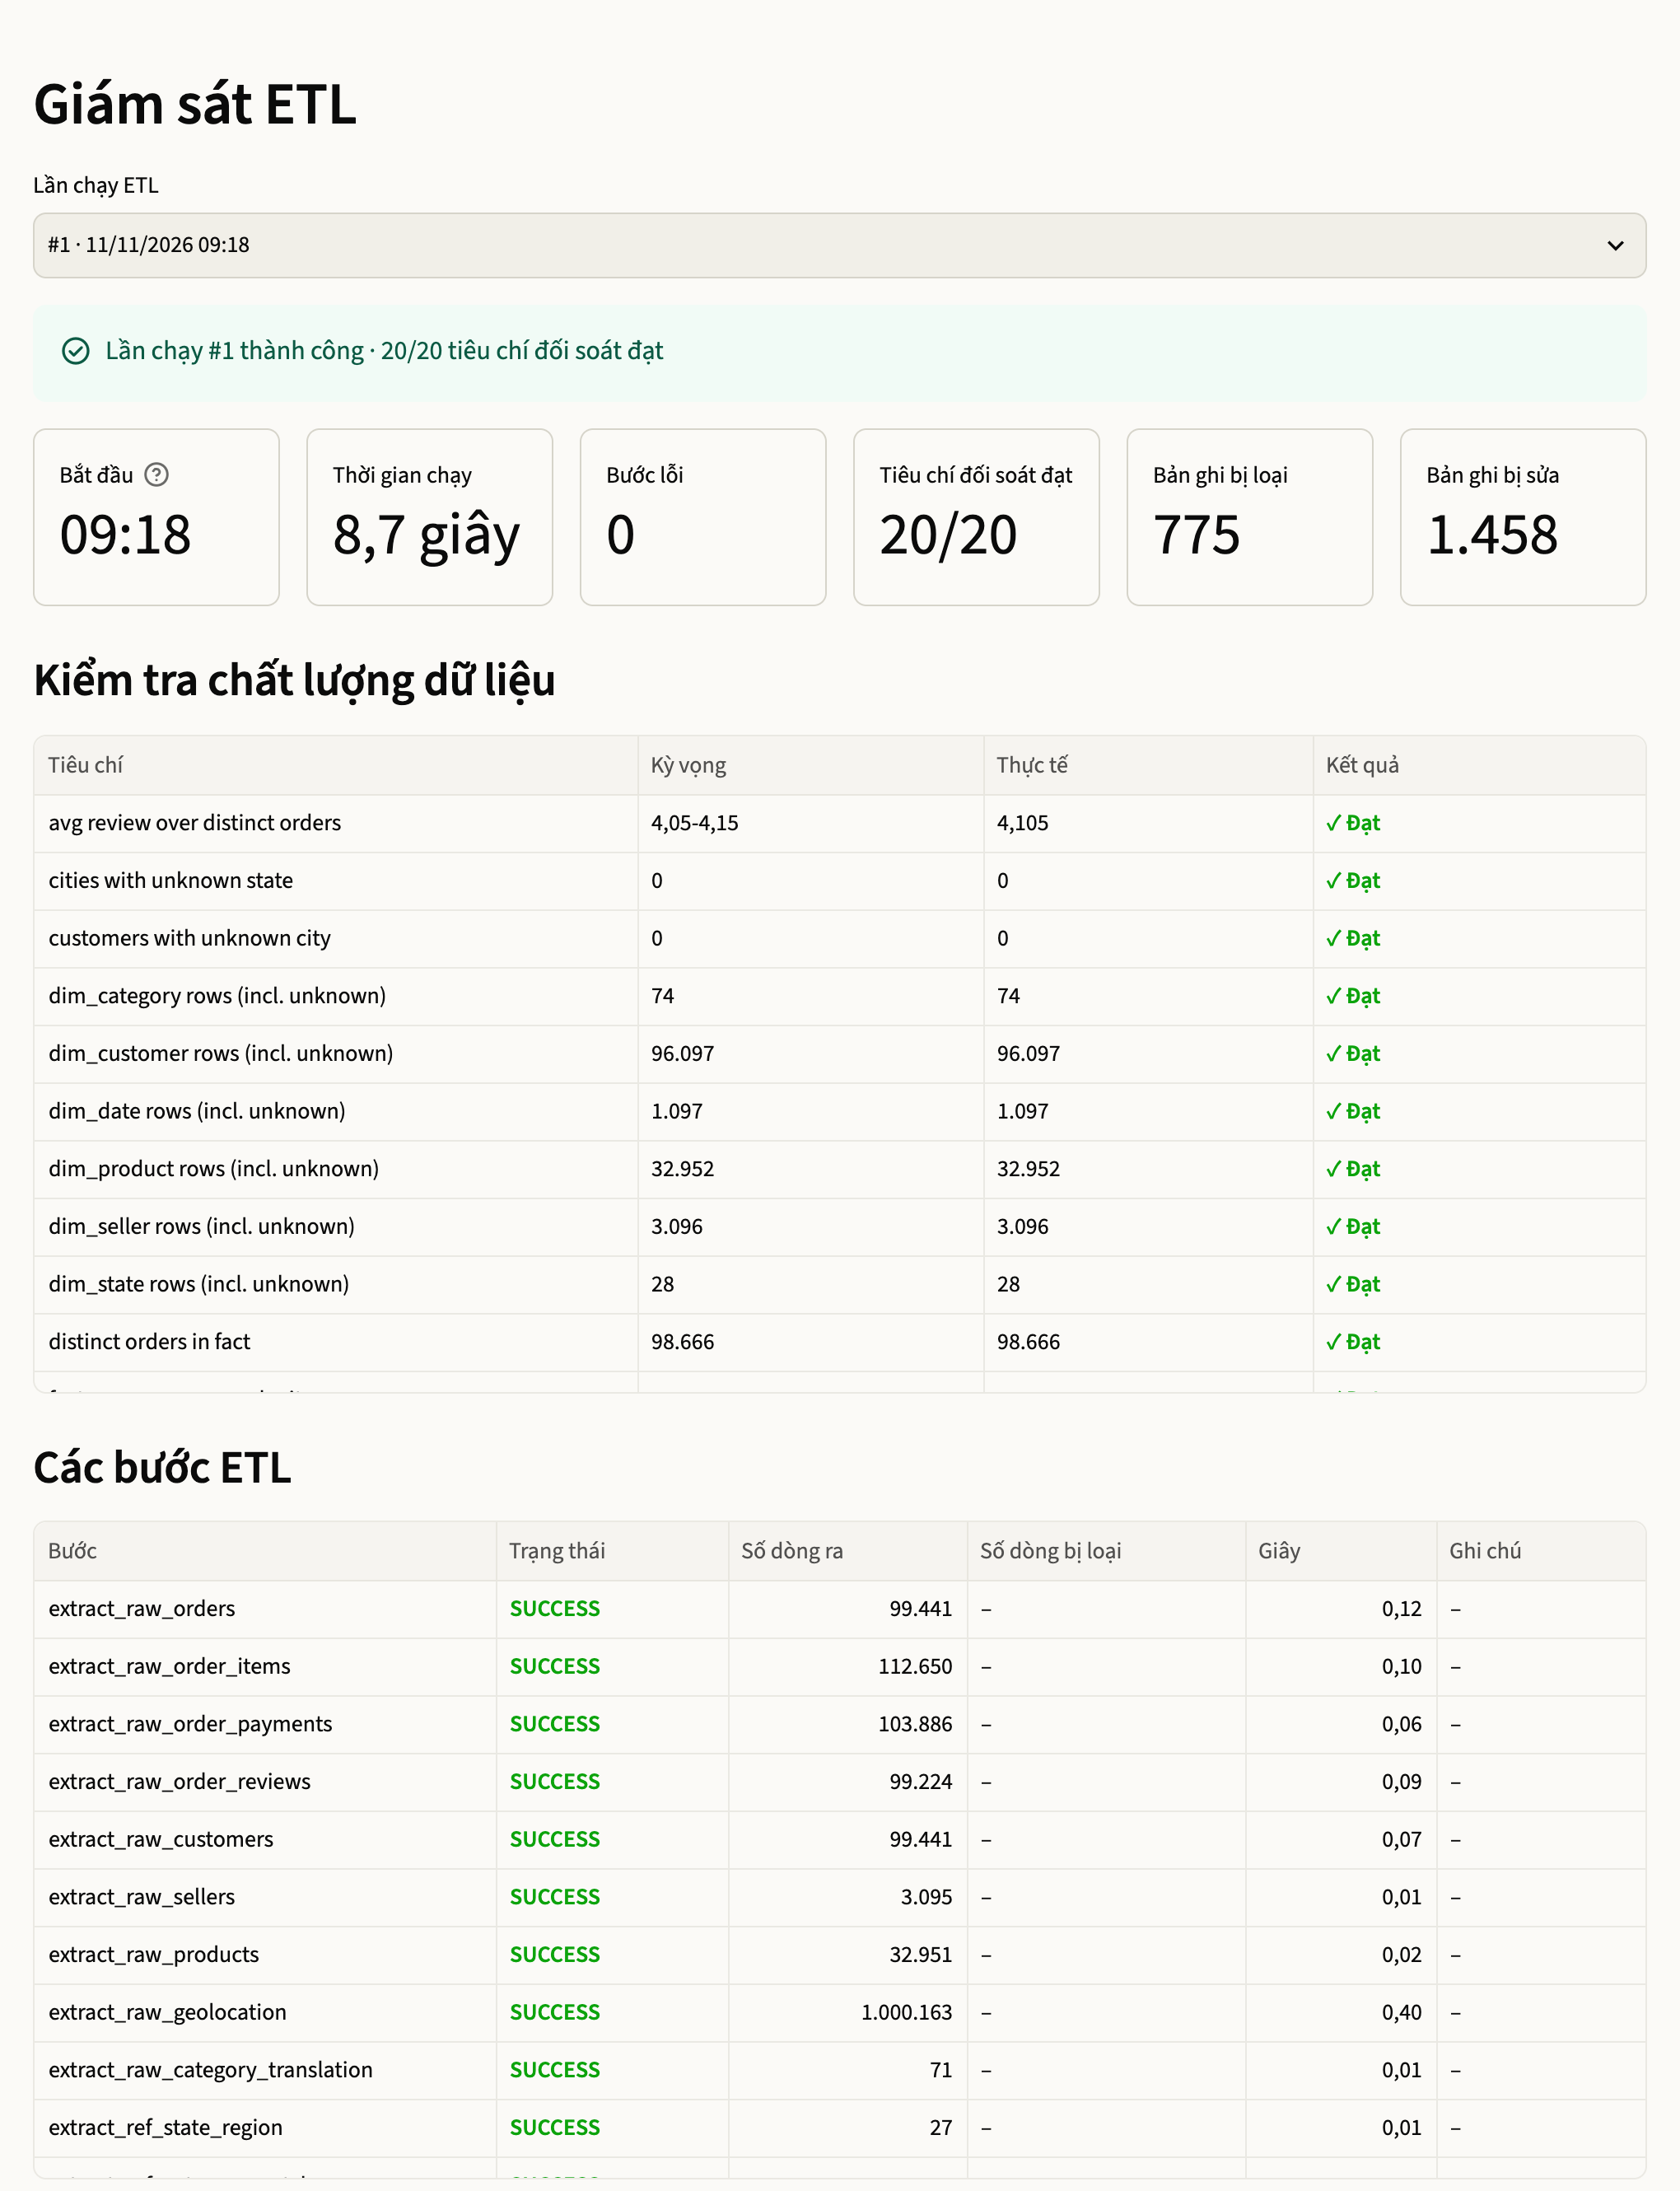
\includegraphics[width=\linewidth]{Pictures/dash-etl.png}
\caption{Trang Giám sát ETL: trạng thái lần chạy, các chỉ số chính, kết quả kiểm tra chất lượng dữ liệu và các bước}
\label{fig:dashetl}
\end{figure}

Trang Cảnh báo giao trễ là giao diện của hệ hỗ trợ quyết định, được trình bày cùng phần DSS ở mục~\ref{sec:dsstrienkhai} (Hình~\ref{fig:dashdsswhatif} và Hình~\ref{fig:dashdssdanhsach}).

\subsubsection{Đối chiếu số liệu và thời gian phản hồi}

Để kiểm tra dashboard tính đúng, các con số trên dashboard được đặt cạnh kết quả truy vấn OLAP và DSS đã trình bày trong báo cáo (Bảng~\ref{tab:doichieu}). Doanh thu và tỷ lệ trễ còn được tính lại bằng pandas trực tiếp từ các tập tin CSV gốc, không qua cơ sở dữ liệu, và cho cùng kết quả.

\begin{table}[H]
\centering
\small\setstretch{1.1}
\caption{Đối chiếu số liệu trên dashboard với kết quả OLAP và DSS}
\label{tab:doichieu}
\begin{tabularx}{\linewidth}{|>{\raggedright\arraybackslash}X|P{2.6cm}|P{3.0cm}|P{3.0cm}|}
\hline
\textbf{Chỉ số} & \textbf{Trang} & \textbf{Trong báo cáo} & \textbf{Trên dashboard}\\ \hline
Doanh thu 2016-2018, không tính đơn hủy hoặc không có hàng & Tổng quan & 13.494.400,74 BRL; 98.199 đơn (Bảng~\ref{tab:rollup}) & 13.494.400,74 BRL; 98.199 đơn\\ \hline
Tỷ lệ giao trễ toàn quốc & Tổng quan, Giao hàng & 6,77\% (Bảng~\ref{tab:drilldown}) & 6,77\%\\ \hline
Tỷ lệ giao trễ bang RJ / SP & Giao hàng & 12,11\% / 4,49\% (Bảng~\ref{tab:drilldown}) & 12,11\% / 4,49\%\\ \hline
Điểm đánh giá TB đơn đúng hạn / đơn trễ & Mức độ hài lòng & 4,29 / 2,27 (mục~\ref{sec:olapnghiepvu}) & 4,29 / 2,27\\ \hline
Doanh thu Sudeste năm 2018 (slice) & Doanh thu & 4.866.163,13 BRL; 66,3\% (Bảng~\ref{tab:slice}) & 4.866.163,13 BRL; 66,3\%\\ \hline
Người bán doanh thu cao, chất lượng thấp & Người bán & 12 người bán (mục~\ref{sec:olapnghiepvu}) & 12 người bán\\ \hline
Tỷ lệ trễ thực tế của đơn mức ĐỎ & Cảnh báo giao trễ & 30,8\% (Bảng~\ref{tab:dsschinhsach}) & 30,8\%\\ \hline
Chính sách chi phí kỳ vọng, tham số mặc định & Cảnh báo giao trễ & $p^{*} = 0{,}667$; 238 đơn; precision 89,1\%; lợi ích ròng 640 BRL & $p^{*} = 0{,}667$; 238 đơn; precision 89,1\%; lợi ích ròng 640 BRL\\ \hline
\end{tabularx}
\end{table}

Cả tám chỉ số đều khớp đến chữ số cuối. Điều này cũng xác nhận quy ước về grain được giữ đúng: nếu tính tỷ lệ trễ trên các dòng của \code{fact\_sales} thay vì trên \code{v\_order}, các đơn nhiều sản phẩm bị đếm lặp và kết quả sẽ lệch khỏi 6,77\%.

Thời gian phản hồi của mỗi trang được đo bằng công cụ kiểm thử AppTest của Streamlit, trong một tiến trình mới chưa có bộ nhớ đệm. Lần mở đầu tiên mất 0,4-1,4 giây ở sáu trang; trang Giao hàng chậm nhất với 4,7 giây vì chạy sáu truy vấn, trong đó có ma trận tuyến và thời gian từng công đoạn. Mở lại trang hoặc quay về bộ lọc đã xem chỉ mất dưới 0,1 giây nhờ bộ nhớ đệm. Như vậy mọi trang đều mở xong trong dưới 5 giây, kể cả lần đầu.


\clearpage
% !TeX root = ../main.tex
\section{Hệ hỗ trợ quyết định}\label{sec:dss}

Phần OLAP ở mục~\ref{sec:olap} cho nhà quản lý biết chuyện gì đã xảy ra: 6,77\% đơn hàng bị giao trễ, và đơn trễ bị chấm trung bình 2,27 điểm so với 4,29 điểm của đơn đúng hạn. Nhưng biết tỷ lệ trễ của tháng trước không giúp bộ phận vận hành xử lý những đơn đang trên đường. Phần này trình bày thành phần hệ hỗ trợ quyết định (DSS) xây dựng trên kho dữ liệu để trả lời một câu hỏi cụ thể: \textit{khi người bán vừa bàn giao đơn hàng cho đơn vị vận chuyển, đơn nào có nguy cơ giao trễ, và sàn nên chủ động xử lý những đơn nào}.

\subsection{Cách tiếp cận}

DSS của đề tài là một DSS hướng mô hình (model-driven), gồm ba thành phần:
\begin{itemize}
    \item \textbf{Dữ liệu:} Data Mart đã xây dựng ở các phần trước.
    \item \textbf{Mô hình:} mô hình Gradient Boosting dự báo xác suất trễ của từng đơn; luật chọn $k$ đơn rủi ro cao nhất khi mỗi ngày chỉ xử lý được $k$ đơn; và mô hình chi phí kỳ vọng kèm phân tích what-if theo các giả định chi phí. Các mô hình được huấn luyện lại mỗi tháng.
    \item \textbf{Giao diện:} trang DSS trên dashboard, nơi người vận hành xem danh sách đơn rủi ro, lý do và hành động đề xuất, rồi duyệt hoặc từ chối từng đề xuất.
\end{itemize}

Quá trình xây dựng DSS đi theo bốn giai đoạn ra quyết định: nhận diện vấn đề (intelligence), thiết kế phương án (design), lựa chọn (choice) và thực hiện (implementation). Bảng~\ref{tab:simon} tóm tắt nội dung của từng giai đoạn; các mục tiếp theo đi lần lượt qua từng giai đoạn.

\begin{table}[H]
\centering
\small\setstretch{1.1}
\caption{Bốn giai đoạn ra quyết định áp dụng cho bài toán giao trễ}
\label{tab:simon}
\begin{tabularx}{\linewidth}{|P{2.9cm}|>{\raggedright\arraybackslash}X|P{3.0cm}|}
\hline
\textbf{Giai đoạn} & \textbf{Nội dung trong đề tài} & \textbf{Mục}\\ \hline
Intelligence -- nhận diện vấn đề & Giao trễ làm tỷ lệ đánh giá 1-2 sao tăng từ 9,3\% lên 62,4\%; nguy cơ trễ tăng mạnh khi người bán chuẩn bị hàng lâu và khi đi xa & \ref{sec:edasach}, \ref{sec:olapnghiepvu}, \ref{sec:dssvande}\\ \hline
Design -- thiết kế phương án & Thời điểm can thiệp, các hành động có thể làm, mô hình dự báo xác suất trễ và mô hình chi phí & \ref{sec:dssmohinh}, \ref{sec:dssketqua}\\ \hline
Choice -- lựa chọn & Chọn đơn can thiệp theo năng lực xử lý hoặc theo chi phí kỳ vọng; người dùng chỉnh giả định chi phí (what-if) & \ref{sec:dsschinhsach}\\ \hline
Implementation -- thực hiện & Chấm điểm hằng ngày, ghi kết quả vào schema \code{dss}, người vận hành phê duyệt, huấn luyện lại hằng tháng & \ref{sec:dsstrienkhai}\\ \hline
\end{tabularx}
\end{table}

\subsection{Nhận diện vấn đề và chỉ tiêu}\label{sec:dssvande}

Kết quả khám phá dữ liệu và OLAP cho thấy ba điều. Thứ nhất, giao trễ là nguyên nhân rõ nhất của đánh giá xấu (Hình~\ref{fig:trevadanhgia}). Thứ hai, giao trễ không phân bố đều: có tuyến trễ 1,1\%, có tuyến trễ 23,7\% (Hình~\ref{fig:tuyengiao}); tuần Black Friday trễ gấp ba bình thường (Hình~\ref{fig:blackfriday}). Thứ ba, khi người bán chuẩn bị hàng quá 10 ngày, tỷ lệ trễ lên tới 29,4\% (Hình~\ref{fig:trenhom}). Những điều này cho thấy có thể dự báo trước, ở một mức nào đó, đơn nào dễ trễ.

Thời điểm dự báo được chọn là \textit{lúc người bán bàn giao đơn cho đơn vị vận chuyển}. Lúc này sàn đã biết người bán chuẩn bị hàng nhanh hay chậm, tín hiệu mạnh nhất tìm được ở phần EDA, mà vẫn còn trung vị 21 ngày tới ngày giao dự kiến để làm gì đó: chủ động báo cho khách, tặng voucher hoặc chuyển sang gói vận chuyển nhanh. Mỗi hành động đều có chi phí, và bộ phận vận hành chỉ xử lý được một số đơn mỗi ngày. Quyết định cần hỗ trợ vì vậy là: \textit{mỗi ngày, trong các đơn vừa được bàn giao, chọn những đơn nào để can thiệp}. Hình~\ref{fig:dssflow} là luồng tổng thể của DSS.

% !TeX root = ../../main.tex
% Luồng của thành phần hỗ trợ quyết định: cảnh báo giao trễ lúc bàn giao vận chuyển
\begin{figure}[H]
\centering
\resizebox{\linewidth}{!}{%
\begin{tikzpicture}[
    b/.style={dwbox=#1, text width=2.55cm, minimum height=1.35cm, font=\scriptsize}]
\node[dwdb=dwBlue, minimum width=2.4cm, minimum height=1.6cm, text width=2.2cm, font=\scriptsize] (dm) at (0,0)
  {\textbf{Data Mart}\\\texttt{fact\_sales}\\+ 7 bảng chiều};
\node[b=dwInkTwo, text width=2.75cm, minimum height=2.3cm] (ft) at (3.3,0)
  {\textbf{Đặc trưng point-in-time}\\[1pt] thời gian chuẩn bị hàng, số ngày còn lại, cam kết giao, tuyến, khoảng cách, tỷ lệ trễ gần đây\\[1pt]
   \textcolor{dwMuted}{chỉ dùng thông tin đã biết lúc bàn giao}};
\node[b=dwBlue, text width=2.6cm, minimum height=2.3cm] (m) at (6.85,0)
  {\textbf{Mô hình dự báo}\\[1pt] Gradient Boosting\\+ luật ``đã quá hạn''\\[1pt] $\rightarrow$ P(trễ), mức rủi ro, 3 lý do};
\node[b=dwYellow, text width=2.75cm, minimum height=2.3cm] (pol) at (10.35,0)
  {\textbf{Chính sách quyết định}\\[1pt] theo năng lực: top 5\% (ĐỎ), 5-15\% (VÀNG) mỗi ngày\\[1pt]
   theo chi phí: $p \cdot C_{\text{trễ}} \cdot e > C_{\text{can thiệp}}$};
\node[b=dwBlue, text width=2.3cm, minimum height=2.3cm] (a) at (13.65,0)
  {\textbf{Hành động đề xuất}\\[1pt] báo trước cho khách, voucher, vận chuyển nhanh};
\node[b=dwInkTwo, text width=2.3cm, minimum height=1.1cm] (hu) at (13.65,-3.4) {Người vận hành phê duyệt / từ chối};
\node[dwdb=dwOrange, minimum width=2.6cm, minimum height=1.25cm, text width=2.4cm, font=\scriptsize] (out) at (9.9,-3.4)
  {\textbf{schema \texttt{dss}}\\điểm rủi ro,\\nhật ký quyết định};
\node[b=dwInkTwo, text width=3.0cm, minimum height=1.1cm, draw=dwMuted, dashed] (re) at (3.3,-3.4)
  {\textbf{Huấn luyện lại hằng tháng}\\chỉ dùng đơn đã biết kết quả};
\draw[dwarrow] (dm) -- (ft);
\draw[dwarrow] (ft) -- (m);
\draw[dwarrow] (m) -- (pol);
\draw[dwarrow] (pol) -- (a);
\draw[dwarrow] (a) -- (hu);
\draw[dwarrow] (hu) -- node[dwlabel, above=1pt] {ghi lại} (out);
\draw[dwarrow] (pol.south) -- node[dwlabel, right=1pt] {điểm rủi ro} (pol.south |- out.north);
\draw[dwdash, rounded corners=3pt] (dm.south) |- node[dwlabel, pos=0.3, left=1pt] {kết quả thực tế} (re.west);
\draw[dwdash, rounded corners=3pt] (re.east) -| (m.south);
\end{tikzpicture}}
\caption{Luồng của thành phần hỗ trợ quyết định: dự báo nguy cơ trễ lúc bàn giao vận chuyển, chính sách quyết định và vòng huấn luyện lại}
\label{fig:dssflow}
\end{figure}


Để biết DSS có đủ tốt để dùng hay không, bốn chỉ tiêu định lượng được đặt ra trước khi huấn luyện (Bảng~\ref{tab:chitieu}). Chỉ tiêu chính gắn với năng lực của đội vận hành: giả sử mỗi ngày đội xử lý được khoảng 10\% số đơn bàn giao, thì danh sách 10\% đơn rủi ro nhất phải chứa ít nhất 40\% số đơn sẽ trễ, tức gấp bốn lần chọn ngẫu nhiên. Mức 10\% được chọn vì gần với tỷ lệ trễ thực tế (6,77\%), nên danh sách đủ dài để bao phần lớn đơn trễ mà vẫn vừa sức một đội nhỏ; mục~\ref{sec:dsschinhsach} xét thêm các mức năng lực khác.

\begin{table}[H]
\centering
\small\setstretch{1.1}
\caption{Các chỉ tiêu của mô hình dự báo giao trễ}
\label{tab:chitieu}
\begin{tabularx}{\linewidth}{|P{1.1cm}|>{\raggedright\arraybackslash}X|P{3.4cm}|}
\hline
\textbf{STT} & \textbf{Chỉ tiêu} & \textbf{Ngưỡng}\\ \hline
1 & Tỷ lệ đơn trễ bắt được khi cảnh báo 10\% đơn rủi ro nhất, trung bình tập test & $\geq 40\%$\\ \hline
2 & Khả năng phân biệt đơn trễ và đơn đúng hạn (ROC-AUC) trên tập test & $\geq 0{,}70$\\ \hline
3 & Độ ổn định: tỷ lệ đơn trễ bắt được ở mức 10\% trong từng tháng test & $\geq 30\%$ mọi tháng\\ \hline
4 & Mức rủi ro có ý nghĩa: tỷ lệ trễ thực tế của đơn mức ĐỎ so với đơn mức XANH & gấp ít nhất 5 lần\\ \hline
\end{tabularx}
\end{table}

\subsection{Dữ liệu và đặc trưng}\label{sec:dssmohinh}

\subsubsection{Nhãn và dữ liệu huấn luyện}

Nhãn của bài toán là cờ \code{is\_late} trong bảng fact. Tập huấn luyện được dựng theo hai quy tắc, để mô hình không dùng thông tin mà sàn chưa có tại lúc dự báo.

Quy tắc thứ nhất xử lý các đơn chưa giao. Tại thời điểm dữ liệu dừng (17/10/2018), 1.694 đơn chưa đến tay khách dù đã quá ngày giao dự kiến. Cờ \code{is\_late} của các đơn này để trống vì chưa có ngày nhận hàng, nhưng thực tế chúng chắc chắn trễ, nên được gán nhãn trễ; nếu bỏ đi, các tháng cuối sẽ trông như ít trễ hơn thực tế. Sau bước này có 97.897 đơn có nhãn, tỷ lệ trễ 8,40\%.

Quy tắc thứ hai xác định lúc nào một nhãn được dùng. Ở tháng $M$, sàn chỉ biết một đơn cũ có trễ hay không khi ngày giao dự kiến của đơn đó đã qua: hoặc đơn đã đến tay khách trước hạn, hoặc đã quá hạn mà chưa đến. Vì vậy tập huấn luyện của tháng $M$ chỉ gồm các đơn có ngày giao dự kiến trước ngày đầu tháng $M$. Nếu chỉ lọc theo ngày nhận hàng, trong các đơn gần đây thì đơn giao sớm đã có nhãn còn đơn trễ thì chưa, và mô hình sẽ học sai rằng đơn gần đây thường đúng hạn.

\subsubsection{Đặc trưng}

Mọi đặc trưng được tính từ Data Mart và chỉ dùng thông tin đã biết tại lúc bàn giao (point-in-time). Các tỷ lệ lịch sử của người bán, tuyến hay bang chỉ tính từ những đơn mà kết quả đã biết trước ngày đặt của đơn đang xét, và được làm mượt về tỷ lệ chung khi có ít đơn. Bảng~\ref{tab:dactrungdss} liệt kê các nhóm đặc trưng.

\begingroup\small\setstretch{1.1}
\begin{longtable}{|P{3.3cm}|>{\raggedright\arraybackslash}p{10.4cm}|}
\caption{Các nhóm đặc trưng của mô hình dự báo giao trễ}\label{tab:dactrungdss}\\
\hline
\textbf{Nhóm} & \textbf{Đặc trưng}\\ \hline \endfirsthead
\hline
\textbf{Nhóm} & \textbf{Đặc trưng}\\ \hline \endhead
Khâu chuẩn bị hàng & Thời gian chuẩn bị thực tế, chênh lệch so với thời gian chuẩn bị thường lệ của người bán, số ngày còn lại tới hạn khi bàn giao, thứ bàn giao\\ \hline
Cam kết giao hàng & Số ngày hứa giao (ngày dự kiến $-$ ngày mua); số ngày dư so với thời gian giao thường lệ của tuyến\\ \hline
Địa lý & Bang, vùng của khách và người bán; giao liên bang; khoảng cách Haversine giữa hai thành phố\\ \hline
Đơn hàng & Số sản phẩm, số người bán, giá trị, phí vận chuyển, khối lượng, thể tích, ngành hàng chính, thời gian duyệt\\ \hline
Thời điểm & Tháng, thứ trong tuần, số ngày tới Black Friday\\ \hline
Lịch sử & Tỷ lệ trễ từ trước tới nay của người bán, tuyến, bang khách; số đơn trước đó của người bán và tuyến\\ \hline
Diễn biến gần đây & Tỷ lệ trễ toàn sàn 7 và 30 ngày qua; tỷ lệ trễ 90 ngày của tuyến và người bán; tải đơn của sàn và người bán trong 7 ngày\\ \hline
Đơn tồn đọng & Trong các đơn đã bàn giao 45 ngày qua, tỷ lệ đơn đã quá hạn mà vẫn chưa giao, tính tại ngày bàn giao cho toàn sàn, theo bang khách và theo tuyến\\ \hline
\end{longtable}
\endgroup

Nhóm đặc trưng ``diễn biến gần đây'' cần thiết vì tỷ lệ trễ của các đơn bàn giao biến động rất mạnh giữa các tháng: 14,7\% ở tháng 02/2018, 20,3\% ở tháng 03/2018 nhưng chỉ 1,8\% ở tháng 06/2018 (Hình~\ref{fig:dsstheothang}a). Tỷ lệ lịch sử từ trước tới nay làm mờ đi những đợt biến động này, còn tỷ lệ trễ của 7-30 ngày gần nhất phản ánh ngay khi cả sàn đang gặp sự cố vận chuyển. Ngày nhận hàng, trạng thái đơn, điểm đánh giá và thời gian vận chuyển đều xảy ra sau lúc bàn giao nên bị loại khỏi danh sách đặc trưng; chương trình kiểm tra điều này bằng một câu lệnh \code{assert} ngay khi khởi tạo.

\subsubsection{Cách chia tập và đánh giá}

Dữ liệu có thứ tự thời gian và thay đổi tính chất theo thời gian, nên không thể chia ngẫu nhiên. Cùng một mô hình đơn giản đạt ROC-AUC 0,80 khi chia ngẫu nhiên 80/20 nhưng chỉ 0,59 khi chia theo thời gian, vì khi chia ngẫu nhiên mô hình được học cả từ những tháng nằm sau đơn cần dự báo, điều không thể có trong thực tế.

Mô hình được đánh giá theo kiểu \textit{walk-forward}: với mỗi tháng từ 07/2017 đến 08/2018, mô hình được huấn luyện lại trên dữ liệu đã biết trước tháng đó rồi dự báo cho các đơn của tháng. Năm tháng 01-05/2018 dùng để chọn tham số; ba tháng 06-08/2018, tương ứng khoảng 20\% số đơn cuối cùng, chỉ dùng một lần để báo cáo kết quả. Ba tháng test có 18.753 đơn được bàn giao, trong đó 822 đơn trễ (4,38\%). Với tỷ lệ thấp như vậy, độ chính xác (accuracy) không phải thước đo tốt: đoán ``không trễ'' cho mọi đơn đã đúng 95,6\%. Thước đo chính vì vậy là \textit{tỷ lệ đơn trễ bắt được khi cảnh báo 10\% đơn rủi ro nhất} (một cách chọn ngẫu nhiên sẽ bắt được 10\%), kèm ROC-AUC, PR-AUC và precision, recall, F1 tại các ngưỡng cảnh báo.

\subsection{Kết quả mô hình}\label{sec:dssketqua}

Các phương án được so sánh gồm hai luật đơn giản, Logistic Regression và Gradient Boosting (\code{HistGradientBoostingClassifier} của scikit-learn). Hai luật là xếp hạng theo tỷ lệ trễ lịch sử của tuyến, và xếp hạng theo số ngày còn lại tới hạn khi bàn giao. Với Gradient Boosting, trước hết một lưới tám bộ tham số được thử trên các tháng validation; bộ tốt nhất của lưới này có \code{learning\_rate} = 0,03, \code{max\_leaf\_nodes} = 15 (số nút lá tối đa của một cây) và \code{min\_samples\_leaf} = 200 (số đơn tối thiểu trong một nút lá, giúp hạn chế overfitting). Để kiểm tra xem còn cải thiện được không, một đợt tìm kiếm mở rộng (TK mở rộng) được chạy thêm, cũng chỉ trên các tháng validation: 60 bộ tham số Gradient Boosting cho mỗi bộ đặc trưng, bốn mức điều chuẩn cho Logistic Regression, ba đặc trưng mới về đơn tồn đọng (tỷ lệ đơn đã bàn giao trong 45 ngày qua đã quá hạn mà chưa giao, tính cho toàn sàn, theo bang khách và theo tuyến), và một mô hình kết hợp ba mô hình tốt nhất bằng trung bình thứ hạng. Hình~\ref{fig:dsssosanh} và Bảng~\ref{tab:dssketqua} so sánh các phương án trên tập test.

\begin{figure}[H]
\centering
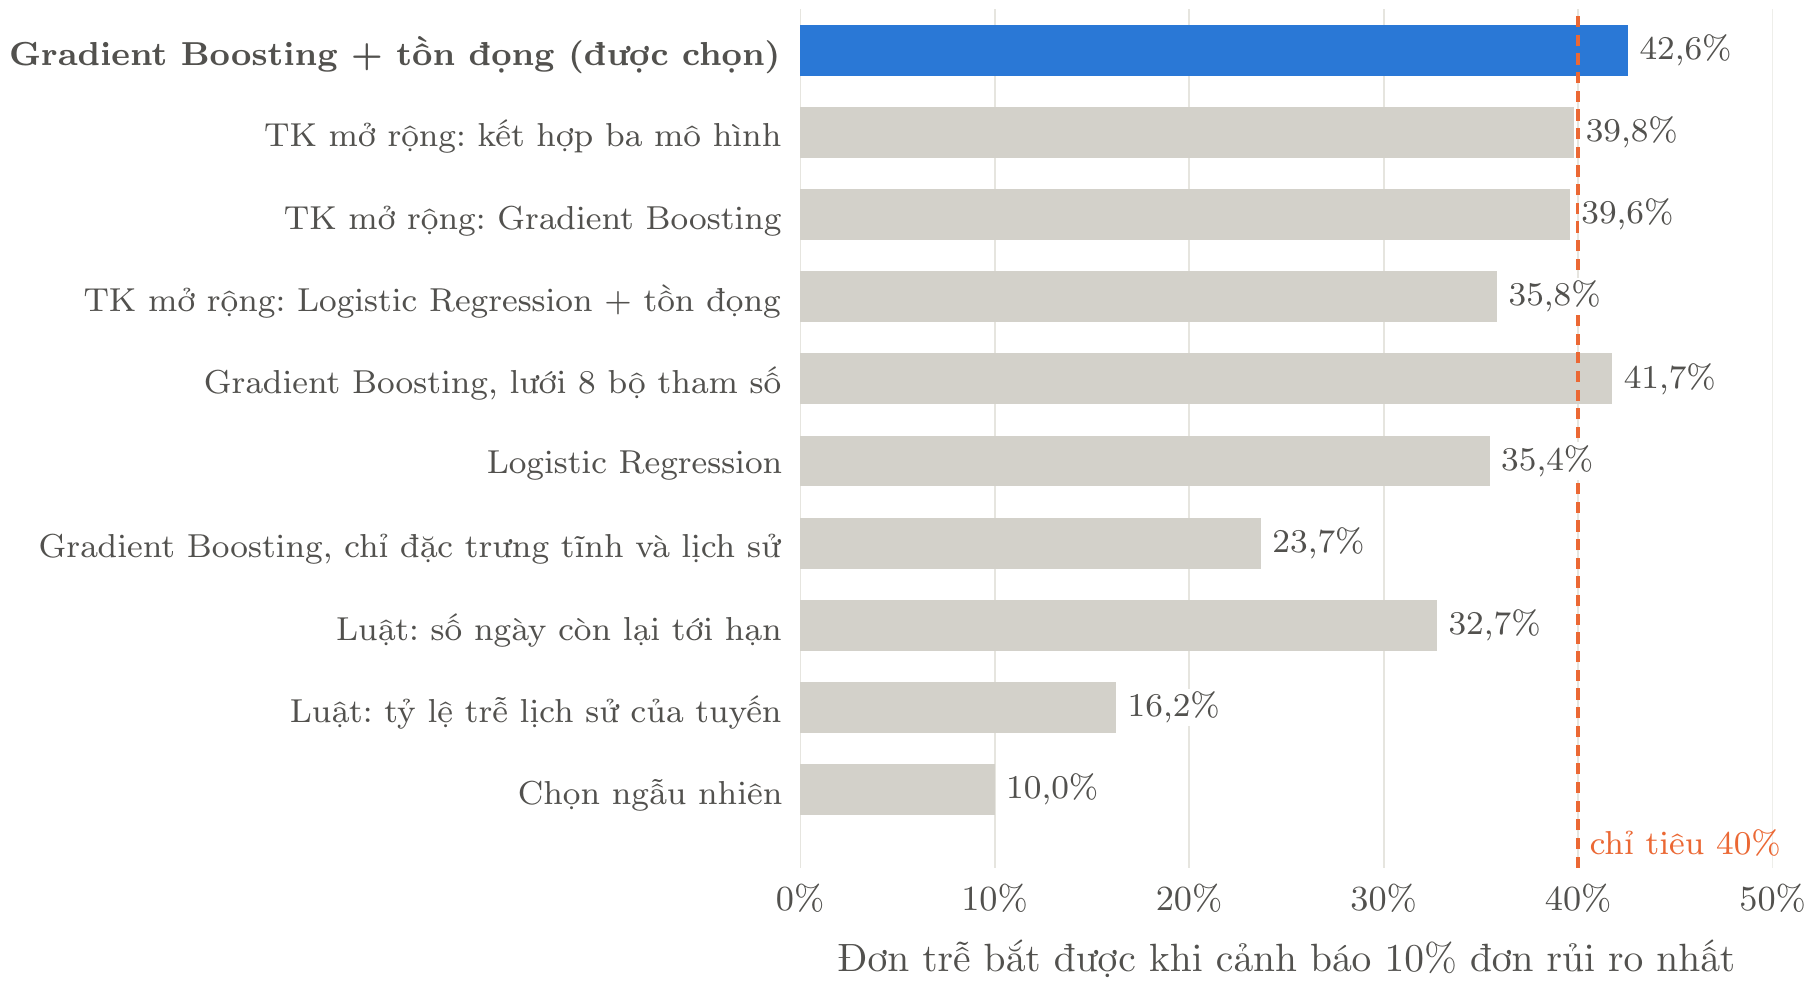
\includegraphics{Pictures/fig-dss-so-sanh-mo-hinh.png}
\caption{Tỷ lệ đơn trễ bắt được khi cảnh báo 10\% đơn rủi ro nhất của các phương án trên tập test 06-08/2018; màu xanh là phương án được chọn}
\label{fig:dsssosanh}
\end{figure}

\begin{table}[H]
\centering
\small\setstretch{1.1}
\caption{Kết quả các phương án trên tập test 06-08/2018 (trung bình ba tháng, huấn luyện lại mỗi tháng); cột cuối là kết quả trên năm tháng validation}
\label{tab:dssketqua}
\begin{tabularx}{\linewidth}{|>{\raggedright\arraybackslash}X|P{1.5cm}|P{1.5cm}|P{2.0cm}|P{2.0cm}|}
\hline
\textbf{Phương án} & \textbf{ROC-AUC} & \textbf{PR-AUC} & \textbf{Bắt được ở 10\% (test)} & \textbf{Bắt được ở 10\% (validation)}\\ \hline
Luật: tỷ lệ trễ lịch sử của tuyến & 0,557 & 0,049 & 16,2\% & 21,4\%\\ \hline
Luật: số ngày còn lại tới hạn & 0,683 & 0,209 & 32,7\% & 10,9\%\\ \hline
Logistic Regression & 0,750 & 0,160 & 35,4\% & 32,3\%\\ \hline
Gradient Boosting, chỉ đặc trưng tĩnh và lịch sử & 0,657 & 0,077 & 23,7\% & 24,0\%\\ \hline
Gradient Boosting, lưới 8 bộ tham số & 0,736 & 0,242 & 41,7\% & 31,9\%\\ \hline
TK mở rộng: Logistic Regression + tồn đọng & 0,749 & 0,162 & 35,8\% & 33,1\%\\ \hline
TK mở rộng: Gradient Boosting & 0,745 & 0,221 & 39,6\% & 33,6\%\\ \hline
TK mở rộng: kết hợp ba mô hình & 0,756 & 0,209 & 39,8\% & 34,3\%\\ \hline
\textbf{TK mở rộng: Gradient Boosting + tồn đọng (được chọn)} & \textbf{0,744} & \textbf{0,254} & \textbf{42,6\%} & \textbf{33,5\%}\\ \hline
\end{tabularx}
\end{table}

Mô hình được chọn bắt được 42,6\% đơn trễ khi chỉ cảnh báo 10\% đơn, gấp hơn bốn lần chọn ngẫu nhiên, với PR-AUC 0,254, gấp 6,8 lần tỷ lệ trễ nền và cao nhất trong các phương án. Logistic Regression có ROC-AUC cao hơn (0,749-0,750), nghĩa là xếp hạng tổng thể tốt tương đương, nhưng ở phần đầu danh sách, phần mà đội vận hành thực sự xử lý, nó chỉ bắt được 35,4-35,8\% đơn trễ; vì quyết định chỉ dựa vào các đơn rủi ro nhất, Gradient Boosting phù hợp hơn. So với cùng thuật toán khi chỉ dùng đặc trưng tĩnh và lịch sử (23,7\%), mức tăng lớn nhất đến từ các đặc trưng lúc bàn giao (thời gian chuẩn bị hàng, số ngày còn lại tới hạn) và các đặc trưng diễn biến gần đây.

Mô hình được chọn không phải phương án cao nhất trên năm tháng validation: vị trí đó thuộc về mô hình kết hợp ba mô hình (34,3\%), nhưng mô hình này chỉ đạt 39,8\% trên test. Năm tháng validation có hai tháng trễ hàng loạt (02 và 03/2018), còn ba tháng test chỉ có khoảng 800 đơn trễ, nên sai số chuẩn của chỉ số vào khoảng $\pm 1{,}7$ điểm phần trăm; chọn theo riêng một giai đoạn ngắn dễ bị nhiễu chi phối. Vì vậy các ứng viên được so sánh trên toàn bộ 14 tháng walk-forward (Bảng~\ref{tab:dsschon}).

\begin{table}[H]
\centering
\small\setstretch{1.1}
\caption{Tỷ lệ đơn trễ bắt được ở mức 10\% của các ứng viên trên từng giai đoạn walk-forward (trung bình theo tháng)}
\label{tab:dsschon}
\begin{tabularx}{\linewidth}{|>{\raggedright\arraybackslash}X|P{1.75cm}|P{1.45cm}|P{1.75cm}|P{1.6cm}|P{1.55cm}|}
\hline
\textbf{Phương án} & \textbf{Validation (5 tháng)} & \textbf{Test (3 tháng)} & \textbf{Năm 2018 (8 tháng)} & \textbf{Cả 14 tháng} & \textbf{ROC-AUC 14 tháng}\\ \hline
Gradient Boosting, lưới 8 bộ tham số & 31,9\% & 41,7\% & 35,6\% & 32,5\% & 0,720\\ \hline
TK mở rộng: Logistic Regression + tồn đọng & 33,1\% & 35,8\% & 34,1\% & 31,5\% & 0,716\\ \hline
TK mở rộng: Gradient Boosting & 33,6\% & 39,6\% & 35,8\% & 32,2\% & 0,728\\ \hline
TK mở rộng: kết hợp ba mô hình & 34,3\% & 39,8\% & 36,4\% & 32,9\% & 0,732\\ \hline
\textbf{TK mở rộng: Gradient Boosting + tồn đọng} & \textbf{33,5\%} & \textbf{42,6\%} & \textbf{36,9\%} & \textbf{33,1\%} & \textbf{0,721}\\ \hline
\end{tabularx}
\end{table}

Gradient Boosting + tồn đọng có kết quả trung bình cao nhất cả trên 14 tháng (33,1\%) lẫn 8 tháng năm 2018 (36,9\%), và tốt hơn mô hình của lưới 8 bộ tham số ở cả bốn giai đoạn; xét từng tháng, nó thắng 8, hòa 2 và thua 4 tháng. Mô hình kết hợp gần ngang về trung bình (32,9\%) và có ROC-AUC tốt hơn, nhưng phải huấn luyện ba mô hình mỗi tháng và kém hơn trên test, nên mô hình đơn được chọn. Vì phép so sánh này có dùng cả ba tháng test, các con số test của mô hình được chọn có thể lạc quan hơn thực tế một chút. Mức tăng so với lưới 8 bộ tham số chủ yếu đến từ bộ tham số mới (\code{learning\_rate} = 0,08, mỗi lần chia nút chỉ xét ngẫu nhiên 50\% đặc trưng) hơn là từ đặc trưng tồn đọng: khi xáo trộn, đặc trưng tồn đọng toàn sàn chỉ làm PR-AUC giảm 0,13 điểm (đứng thứ 10), còn hai đặc trưng tồn đọng theo bang và theo tuyến gần như không đóng góp.

Hình~\ref{fig:dsstheothang} đặt kết quả từng tháng (b) cạnh tỷ lệ trễ của chính tháng đó (a). Ở ba tháng test, mô hình bắt được 40,5\%, 43,0\% và 44,1\% số đơn trễ, ổn định dù tỷ lệ trễ của các tháng này chênh nhau gấp ba (1,8\% ở 06/2018, 5,5\% ở 08/2018). Mô hình của lưới 8 bộ tham số (đường xanh lá) bám sát mô hình được chọn ở hầu hết các tháng; nó nhỉnh hơn ở 10/2017 và 12/2017 nhưng thấp hơn rõ ở 04/2018 (31,6\% so với 37,2\%). Luật theo tuyến chỉ bắt được 6,6\% ở tháng 08/2018, thấp hơn cả chọn ngẫu nhiên.

Đọc hai panel cùng nhau còn thấy một quy luật: đường của mô hình đi xuống đúng vào những tháng cột tỷ lệ trễ vọt lên. Ở 11/2017 và 12/2017 (mùa Black Friday, trễ 12,7\% và 8,2\%) và ở 03/2018 (trễ 20,3\%), mô hình chỉ bắt được 24-27\%. Trong những tháng này đơn trễ hàng loạt vì sự cố chung của khâu vận chuyển chứ không vì đặc điểm riêng của từng đơn, nên việc xếp hạng các đơn với nhau ít tác dụng hơn. Tháng 07/2017 thấp nhất (15,6\%) vì khi đó mới có 11.638 đơn để huấn luyện. Từ 04/2018, khi tập huấn luyện có gần 60 nghìn đơn, kết quả tăng lên 37-44\% và giữ ở mức đó trong cả ba tháng test.

\begin{figure}[H]
\centering
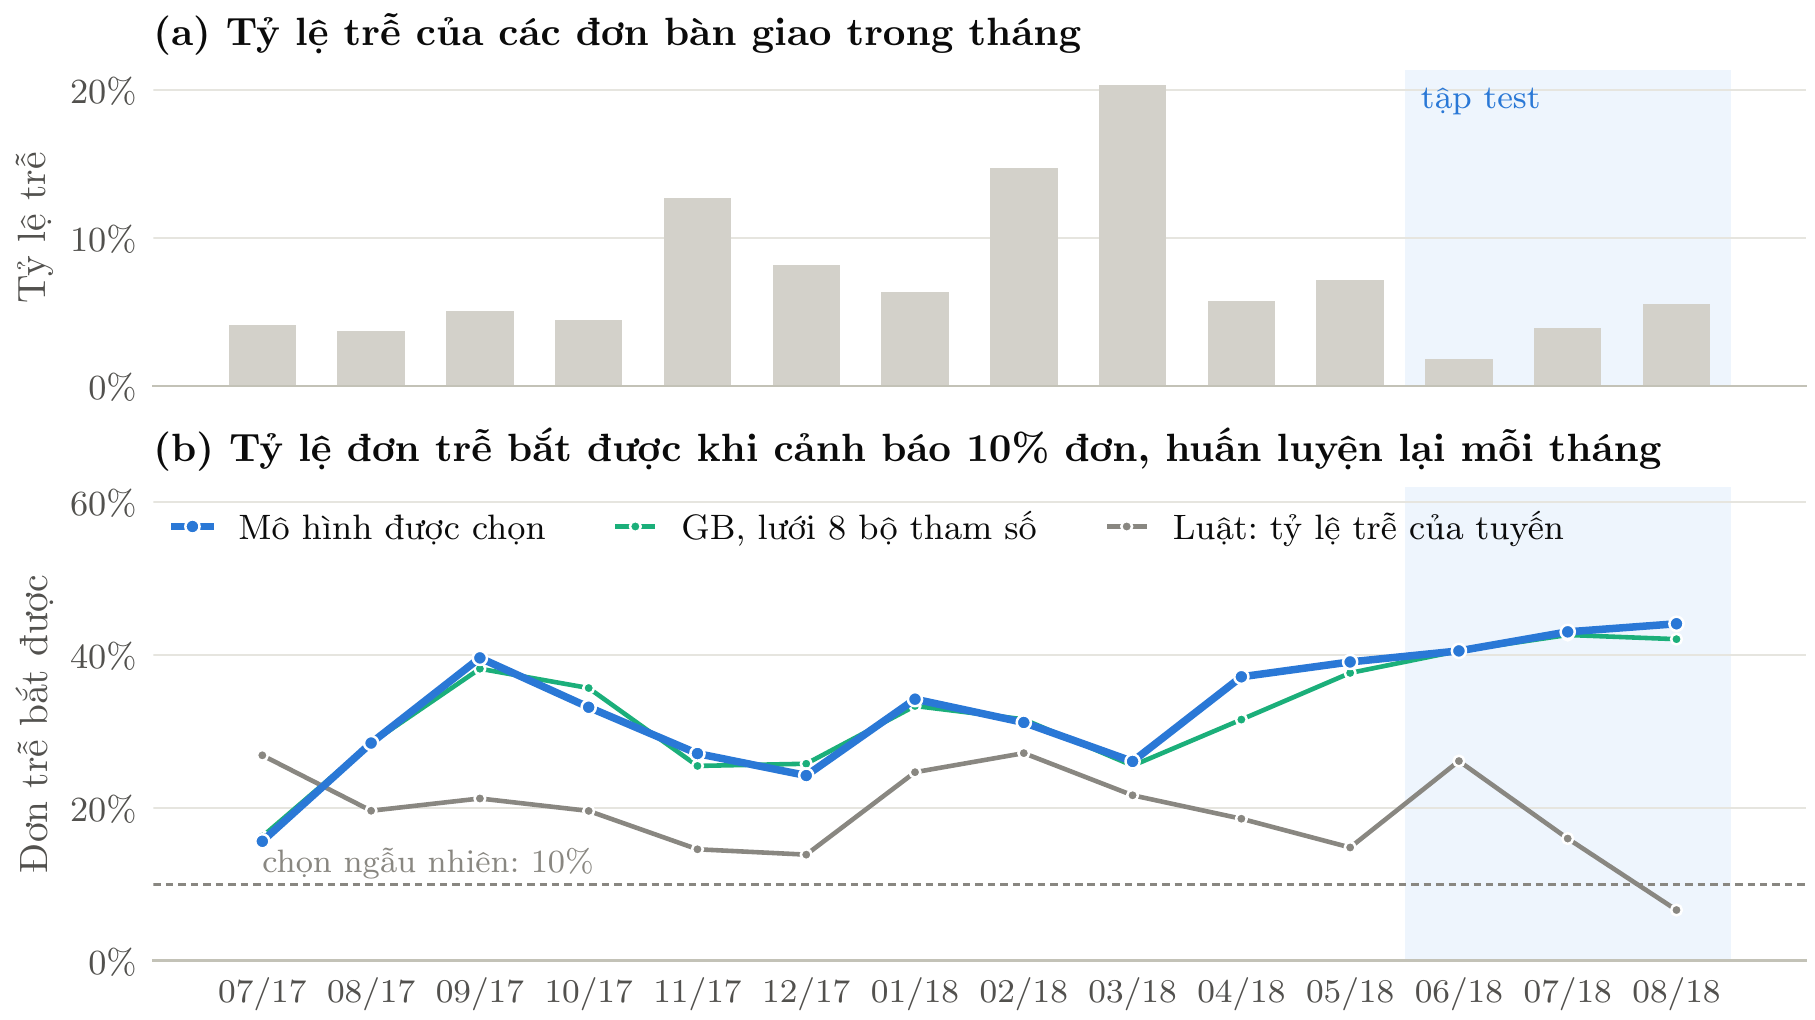
\includegraphics{Pictures/fig-dss-theo-thang.png}
\caption{Tỷ lệ trễ theo tháng (a) và tỷ lệ đơn trễ bắt được khi cảnh báo 10\% đơn, huấn luyện lại mỗi tháng (b); mô hình được chọn là Gradient Boosting (GB) + tồn đọng; vùng tô xanh là tập test}
\label{fig:dsstheothang}
\end{figure}

Bên cạnh mô hình, 120 đơn được bàn giao khi đã quá ngày giao dự kiến (14,6\% số đơn trễ của ba tháng test) được bắt bằng luật mà không cần mô hình, vì các đơn này chắc chắn trễ. Kết hợp mô hình và luật này, DSS bắt được 46,5\% số đơn trễ khi cảnh báo 10\% số đơn bàn giao mỗi ngày.

Để biết mô hình dựa vào đâu, mức giảm PR-AUC được đo khi xáo trộn ngẫu nhiên từng đặc trưng (permutation importance) trên tháng test cuối cùng (Hình~\ref{fig:dssdactrung}). Số ngày còn lại tới hạn khi bàn giao chiếm ưu thế tuyệt đối (PR-AUC giảm 28,8 điểm khi xáo trộn đặc trưng này), cách xa các đặc trưng tiếp theo: thời gian chuẩn bị thực tế (2,0 điểm), người bán chuẩn bị hàng chậm hơn thường lệ của chính họ (1,8 điểm) và độ dư của ngày hứa giao so với thời gian giao thường lệ của tuyến (1,4 điểm). Các đặc trưng còn lại, như tỷ lệ trễ lịch sử của bang khách hay thứ bàn giao, chỉ đóng góp dưới 1 điểm. Kết quả này khớp với phần EDA và với trực giác nghiệp vụ: người bán giữ hàng càng lâu thì đơn vị vận chuyển càng ít thời gian. Đây cũng là cơ sở để sinh các lý do hiển thị cho người vận hành ở mục~\ref{sec:dsstrienkhai}.

\begin{figure}[H]
\centering
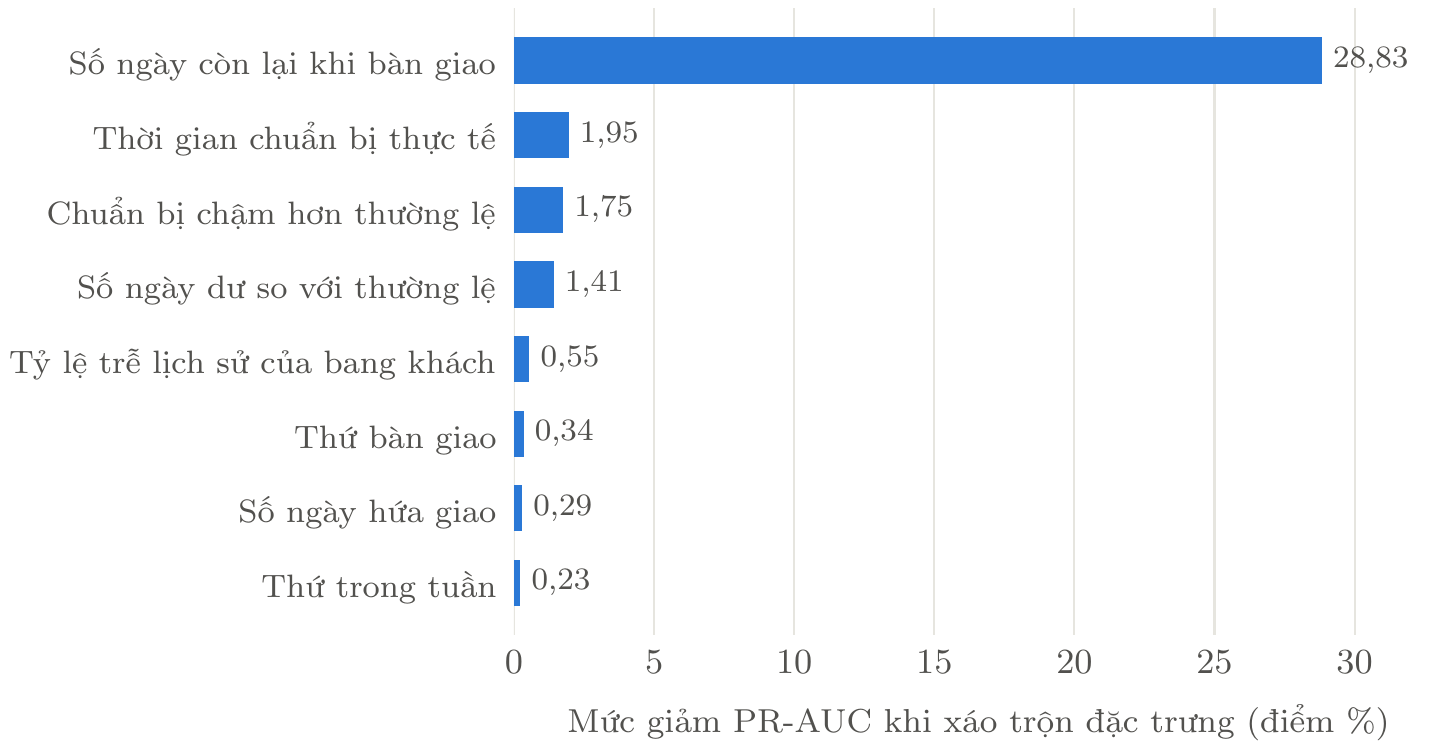
\includegraphics{Pictures/fig-dss-dac-trung.png}
\caption{Tám đặc trưng quan trọng nhất của mô hình (permutation importance, tháng 08/2018)}
\label{fig:dssdactrung}
\end{figure}

Hình~\ref{fig:dssmatran} là ma trận nhầm lẫn của DSS trên ba tháng test ở hai mức cảnh báo được dùng trong thực tế (mục~\ref{sec:dsschinhsach}). Khi chỉ cảnh báo mức ĐỎ, cứ khoảng ba đơn bị cảnh báo thì có một đơn thật sự trễ (precision 30,8\%: 285 đúng, 640 cảnh báo nhầm), và DSS bắt được 34,7\% số đơn trễ; 537 đơn trễ còn lại không bị cảnh báo. Mở rộng sang cả mức VÀNG thì bắt được 54,0\% (444 đơn) nhưng precision giảm còn 16,0\%. Accuracy ở cả hai mức (93,7\% và 85,5\%) đều thấp hơn mức 95,6\% của cách đoán ``không trễ'' cho mọi đơn, một lần nữa cho thấy vì sao không dùng accuracy để đánh giá bài toán này.

\begin{figure}[H]
\centering
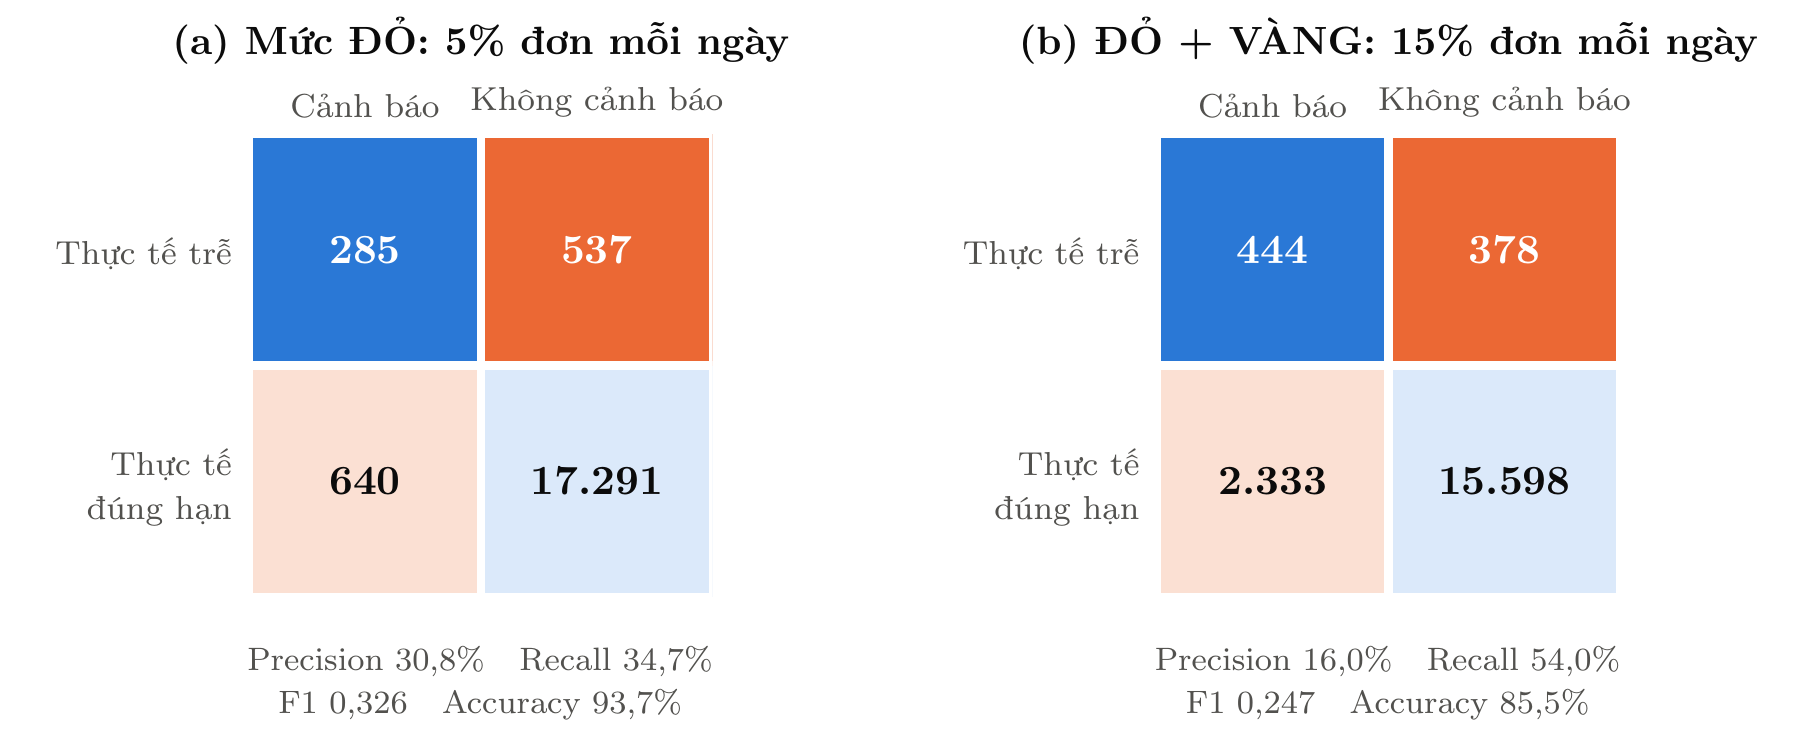
\includegraphics{Pictures/fig-dss-ma-tran-nham-lan.png}
\caption{Ma trận nhầm lẫn của DSS trên 18.753 đơn bàn giao trong ba tháng test, ở hai mức cảnh báo}
\label{fig:dssmatran}
\end{figure}

Bảng~\ref{tab:datchitieu} đối chiếu kết quả với các chỉ tiêu đã đặt ở Bảng~\ref{tab:chitieu}: cả bốn chỉ tiêu đều đạt.

\begin{table}[H]
\centering
\small\setstretch{1.1}
\caption{Đối chiếu kết quả của DSS với các chỉ tiêu}
\label{tab:datchitieu}
\begin{tabularx}{\linewidth}{|>{\raggedright\arraybackslash}X|P{2.4cm}|P{3.6cm}|P{1.4cm}|}
\hline
\textbf{Chỉ tiêu} & \textbf{Ngưỡng} & \textbf{Kết quả} & \textbf{Đánh giá}\\ \hline
Đơn trễ bắt được ở mức 10\% & $\geq 40\%$ & 42,6\% (mô hình); 46,5\% (kèm luật) & Đạt\\ \hline
ROC-AUC trên tập test & $\geq 0{,}70$ & 0,744 & Đạt\\ \hline
Ổn định qua từng tháng test & $\geq 30\%$ mọi tháng & 40,5\%; 43,0\%; 44,1\% & Đạt\\ \hline
Tỷ lệ trễ của mức ĐỎ so với mức XANH & gấp ít nhất 5 lần & 30,8\% so với 2,4\% (13,0 lần) & Đạt\\ \hline
\end{tabularx}
\end{table}

\subsection{Chính sách quyết định}\label{sec:dsschinhsach}

Mô hình chỉ cho ra xác suất trễ. Việc chọn đơn nào để can thiệp là một quyết định trong điều kiện rủi ro: với mỗi đơn ta biết xác suất xảy ra kết quả xấu chứ không biết chắc kết quả. DSS đưa ra hai chính sách để người quản lý chọn tùy tình huống.

\subsubsection{Chính sách theo năng lực xử lý}

Khi đội vận hành chỉ xử lý được một số đơn cố định mỗi ngày, DSS xếp hạng các đơn bàn giao trong ngày theo điểm rủi ro và gán ba mức: ĐỎ cho 5\% đơn rủi ro nhất, VÀNG cho 10\% tiếp theo, XANH cho phần còn lại; mọi đơn đã quá hạn khi bàn giao đều được xếp ĐỎ. Hình~\ref{fig:dssmucruiro} kiểm chứng cách xếp mức này trên ba tháng test: 30,8\% trong 925 đơn ĐỎ thực sự bị trễ, 8,6\% trong 1.852 đơn VÀNG, còn 15.976 đơn XANH chỉ trễ 2,4\%. Tỷ lệ trễ giảm dần đúng theo thứ tự mức rủi ro, và đơn ĐỎ trễ nhiều gấp 13,0 lần đơn XANH; ba mức vì vậy có ý nghĩa thực tế để phân bổ công sức theo dõi.

\begin{figure}[H]
\centering
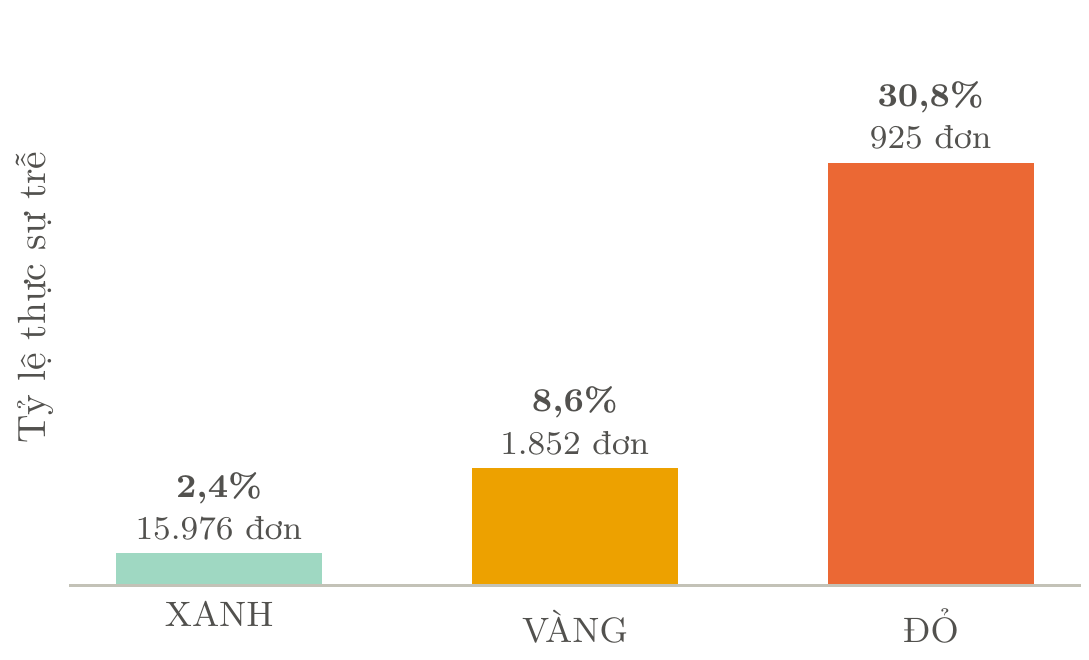
\includegraphics{Pictures/fig-dss-muc-rui-ro.png}
\caption{Tỷ lệ đơn thực sự trễ trong từng mức rủi ro, ba tháng test 06-08/2018}
\label{fig:dssmucruiro}
\end{figure}

Hình~\ref{fig:dssnangluc} cho người quản lý thấy đánh đổi giữa năng lực và hiệu quả: xử lý 5\% đơn mỗi ngày thì bắt được 35\% số đơn trễ, 10\% thì bắt được 47\%, 15\% thì bắt được 54\%, còn 30\% thì bắt được 67\%. Đường cong dốc ở đầu rồi thoải dần, nghĩa là những đơn được xử lý đầu tiên mang lại nhiều giá trị nhất, còn mở rộng năng lực quá 15-20\% thì lợi ích tăng thêm không nhiều.

\begin{figure}[H]
\centering
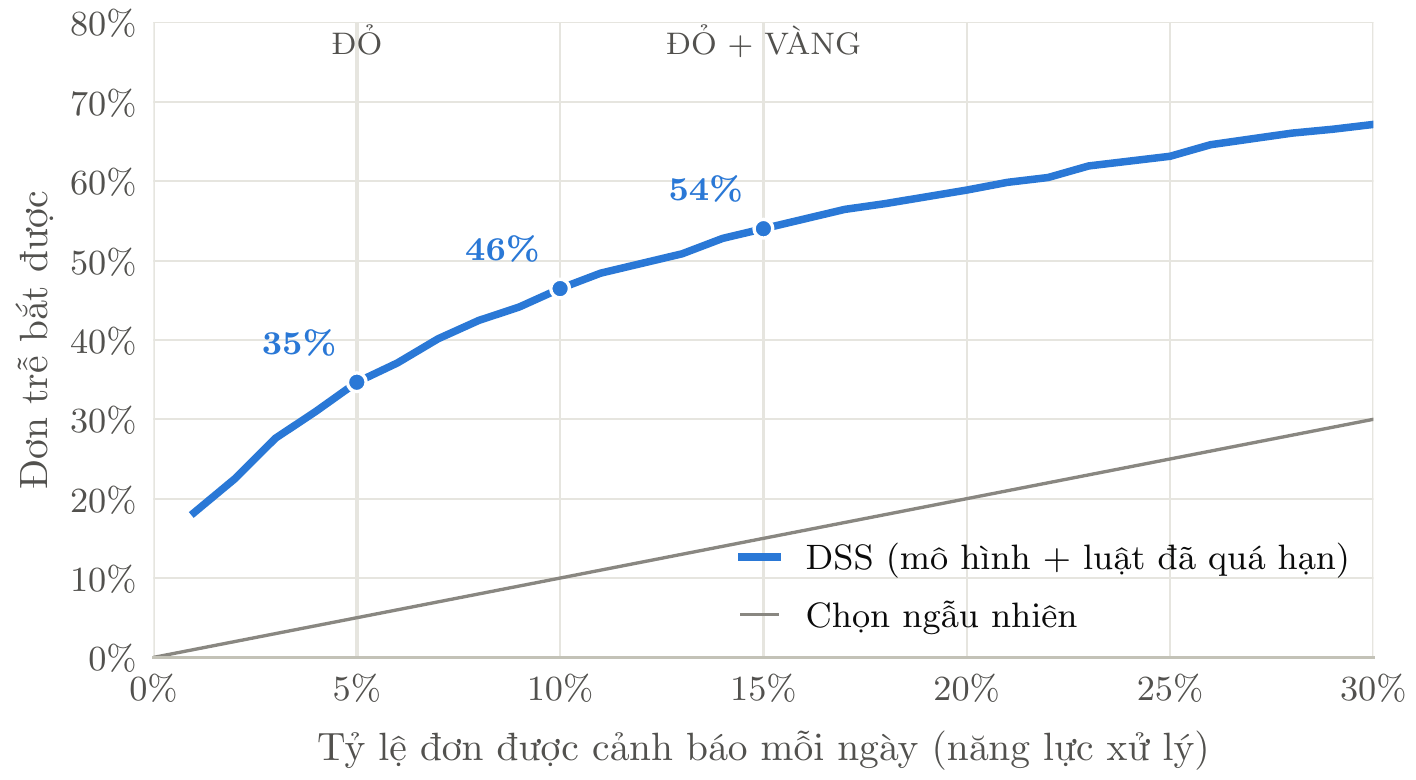
\includegraphics{Pictures/fig-dss-nang-luc.png}
\caption{Tỷ lệ đơn trễ bắt được theo năng lực xử lý mỗi ngày, ba tháng test}
\label{fig:dssnangluc}
\end{figure}

\subsubsection{Chính sách theo chi phí kỳ vọng}

Khi hành động can thiệp tốn tiền, như tặng voucher, nên quyết định theo giá trị kỳ vọng. Gọi $p$ là xác suất trễ (đã hiệu chỉnh bằng isotonic regression trên 60 ngày gần nhất), $C_{\text{trễ}}$ là thiệt hại khi một đơn bị trễ, $e$ là tỷ lệ thiệt hại tránh được nhờ can thiệp và $C_{\text{can thiệp}}$ là chi phí can thiệp một đơn. Can thiệp có lợi khi
\[
p \cdot C_{\text{trễ}} \cdot e > C_{\text{can thiệp}}
\quad\Longleftrightarrow\quad
p > p^{*} = \frac{C_{\text{can thiệp}}}{C_{\text{trễ}} \cdot e}.
\]
Các tham số chi phí không có trong dữ liệu, nên DSS dùng giả định mặc định và cho người dùng chỉnh lại trên dashboard (what-if). Giả định mặc định là $C_{\text{trễ}} = 30$ BRL (khoảng 22\% giá trị đơn trung bình, gồm chi phí hỗ trợ khách và phần giá trị khách hàng có thể mất), hành động là liên hệ khách và tặng voucher với $C_{\text{can thiệp}} = 8$ BRL, $e = 0{,}4$; khi đó $p^{*} = 0{,}667$. Bảng~\ref{tab:dsschinhsach} là kết quả backtest các chính sách trên ba tháng test. Số đánh giá 1-2 sao tránh được được ước tính bằng số đơn trễ bắt được nhân $e$ nhân mức chênh tỷ lệ đánh giá thấp giữa đơn trễ và đơn đúng hạn (62,4\% $-$ 9,3\%).

\begin{table}[H]
\centering
\small\setstretch{1.1}
\caption{Backtest các chính sách quyết định trên ba tháng test (18.753 đơn bàn giao)}
\label{tab:dsschinhsach}
\begin{tabularx}{\linewidth}{|>{\raggedright\arraybackslash}X|P{1.6cm}|P{1.9cm}|P{1.9cm}|P{1.8cm}|P{1.7cm}|}
\hline
\textbf{Chính sách} & \textbf{Số đơn can thiệp} & \textbf{Đơn trễ bắt được} & \textbf{Precision} & \textbf{Lợi ích ròng (BRL)} & \textbf{Đánh giá xấu tránh được}\\ \hline
Mức ĐỎ (5\%) & 925 & 285 (34,7\%) & 30,8\% & $-$3.980 & 61\\ \hline
ĐỎ + VÀNG (15\%) & 2.777 & 444 (54,0\%) & 16,0\% & $-$16.888 & 94\\ \hline
Chi phí kỳ vọng ($p^{*} = 0{,}667$) & 238 & 212 (25,8\%) & 89,1\% & 640 & 45\\ \hline
\end{tabularx}
\end{table}

Bảng~\ref{tab:dsschinhsach} cho thấy điều mà con số dự báo đơn lẻ không nói được. Tặng voucher cho cả 15\% đơn rủi ro nhất lỗ gần 17 nghìn BRL, vì precision 16,0\% chưa đủ bù chi phí; chính sách chi phí kỳ vọng chỉ tặng voucher cho 238 đơn có xác suất trễ cao (precision 89,1\%) và có lãi. Trong 238 đơn này, 120 đơn đến từ luật ``đã quá hạn khi bàn giao'' và 118 đơn do mô hình chọn; 92 trong 118 đơn đó trễ thật (78\%), tức là sau khi hiệu chỉnh, mô hình vẫn tìm thêm được một nhóm đơn rất dễ trễ mà luật không bắt được. Cách hợp lý vì vậy là kết hợp: với các đơn ĐỎ chỉ báo trước cho khách, việc gần như không tốn tiền, còn voucher chỉ dành cho các đơn vượt ngưỡng $p^{*}$. Kết luận này phụ thuộc vào giả định chi phí: chẳng hạn nếu voucher chỉ giữ lại được 20\% thiệt hại ($e = 0{,}2$) thì $p^{*}$ vượt quá 1, DSS chỉ còn đề xuất voucher cho các đơn đã chắc chắn trễ. Vì vậy các tham số này được để mở cho người quản lý chỉnh theo số liệu thực tế của sàn.

\subsection{Triển khai và giao diện}\label{sec:dsstrienkhai}

Ở mỗi kỳ chạy, chương trình \code{score\_delay.py} huấn luyện lại mô hình trên các đơn đã biết kết quả, hiệu chỉnh xác suất, chấm điểm các đơn mới được bàn giao, gán mức rủi ro và ghi vào bảng \code{dss.delay\_risk\_score}; thông tin của từng phiên bản mô hình (dữ liệu huấn luyện, kết quả đánh giá) được lưu ở \code{dss.model\_registry}. Với ba tháng test, bảng điểm có 18.753 dòng ứng với ba phiên bản mô hình.

Để người vận hành hiểu vì sao một đơn bị cảnh báo, mỗi đơn ĐỎ hoặc VÀNG có tối đa ba lý do bằng tiếng Việt. Lý do được sinh từ các đặc trưng quan trọng ở Hình~\ref{fig:dssdactrung}: đặc trưng nào của đơn lệch xa mức bình thường nhất thì được nêu trước. Trong 925 đơn ĐỎ, lý do đứng đầu phổ biến nhất là tỷ lệ trễ cao của tuyến (350 đơn), ngày hứa giao quá sát (181 đơn), người bán chuẩn bị hàng chậm hơn thường lệ (124 đơn), đơn đã quá hạn khi bàn giao (120 đơn) và chỉ còn ít ngày tới hạn (92 đơn). Bảng~\ref{tab:dssvidu} là ba đơn ĐỎ trễ thật và ba đơn ĐỎ vẫn đúng hạn, chọn ngẫu nhiên trong tháng 07/2018. Ba đơn trễ có cùng một kiểu lý do rất rõ: người bán giữ hàng lâu hơn thường lệ 15-21 ngày, khi bàn giao chỉ còn 0-1 ngày tới hạn, và mô hình cho xác suất trễ gần như chắc chắn (1,00). Ba đơn đúng hạn bị cảnh báo chủ yếu vì yếu tố tuyến (tuyến SP$\rightarrow$BA hay trễ, ngày hứa giao sát) hoặc người bán có tỷ lệ trễ gần đây cao, là những yếu tố làm tăng rủi ro nhưng không quyết định; xác suất của chúng chỉ khoảng 0,09-0,19. Người vận hành vì vậy có thể dùng cả mức xác suất lẫn loại lý do để quyết định mức độ can thiệp.

\begingroup\small\setstretch{1.1}
\begin{longtable}{|P{1.6cm}|P{1.0cm}|>{\raggedright\arraybackslash}p{8.2cm}|P{1.6cm}|}
\caption{Ví dụ đầu ra của DSS: ba đơn ĐỎ trễ thật và ba đơn ĐỎ đúng hạn, chọn ngẫu nhiên trong tháng 07/2018}\label{tab:dssvidu}\\
\hline
\textbf{Tuyến} & \textbf{$p$} & \textbf{Lý do hiển thị cho người vận hành} & \textbf{Thực tế}\\ \hline \endfirsthead
\hline
\textbf{Tuyến} & \textbf{$p$} & \textbf{Lý do hiển thị cho người vận hành} & \textbf{Thực tế}\\ \hline \endhead
SP$\rightarrow$MG & 1,00 & Người bán chuẩn bị hàng chậm hơn thường lệ 21 ngày; chỉ còn 1 ngày tới hạn giao khi bàn giao vận chuyển & Trễ\\ \hline
MA$\rightarrow$SP & 1,00 & Người bán chuẩn bị hàng chậm hơn thường lệ 15 ngày; chỉ còn 0 ngày tới hạn giao khi bàn giao vận chuyển; người bán trễ 20\% trong 90 ngày qua & Trễ\\ \hline
MA$\rightarrow$MA & 1,00 & Người bán chuẩn bị hàng chậm hơn thường lệ 17 ngày; chỉ còn 0 ngày tới hạn giao khi bàn giao vận chuyển; người bán trễ 21\% trong 90 ngày qua & Trễ\\ \hline
SP$\rightarrow$BA & 0,16 & Ngày hứa giao sớm hơn thời gian giao thường lệ của tuyến 1 ngày; tuyến SP$\rightarrow$BA trễ 19\% trong 90 ngày qua & Đúng hạn\\ \hline
SP$\rightarrow$BA & 0,09 & Tuyến SP$\rightarrow$BA trễ 19\% trong 90 ngày qua; ngày hứa giao chỉ dư 3 ngày so với thời gian giao thường lệ của tuyến & Đúng hạn\\ \hline
MA$\rightarrow$BA & 0,19 & Người bán trễ 21\% trong 90 ngày qua; người bán chuẩn bị hàng chậm hơn thường lệ 3 ngày; ngày hứa giao chỉ dư 4 ngày so với thời gian giao thường lệ của tuyến & Đúng hạn\\ \hline
\end{longtable}
\endgroup

Kèm theo mỗi mức là một hành động đề xuất: đơn ĐỎ được đề xuất báo trước cho khách, tặng voucher nếu vượt ngưỡng $p^{*}$, hoặc chuyển gói vận chuyển nhanh (mô phỏng, vì dữ liệu không có thông tin đơn vị vận chuyển); đơn VÀNG được theo dõi hành trình hằng ngày. Người vận hành phê duyệt hoặc từ chối từng đề xuất trên dashboard, và quyết định được ghi vào \code{dss.decision\_log} để đánh giá lại về sau. Mô hình được huấn luyện lại mỗi tháng, đúng như cách đã đánh giá ở mục~\ref{sec:dssketqua}.

Trang ``Cảnh báo giao trễ'' của dashboard (mục~\ref{sec:dashboard}) là giao diện của DSS và có hai phần. Phần trên (Hình~\ref{fig:dashdsswhatif}) là phân tích what-if: ba thanh trượt cho $C_{\text{trễ}}$, $C_{\text{can thiệp}}$ và $e$, ô ngưỡng $p^{*}$ tính lại theo giá trị đang chọn (công thức nằm trong chú giải của ô), và bảng so sánh ba chính sách như Bảng~\ref{tab:dsschinhsach}. Với tham số mặc định, trang cho đúng $p^{*} = 0{,}667$, 238 đơn được đề xuất voucher, precision 89,1\% và lợi ích ròng 640 BRL. Khi kéo $C_{\text{trễ}}$ lên 50 BRL và $C_{\text{can thiệp}}$ lên 10 BRL, ngưỡng giảm còn $p^{*} = 0{,}500$ và danh sách đơn được đề xuất voucher cập nhật ngay. Hai biểu đồ phía dưới phần này (không có trên hình) nhắc lại tỷ lệ trễ thực tế theo mức rủi ro (Hình~\ref{fig:dssmucruiro}) và tỷ lệ đơn trễ bắt được theo năng lực xử lý mỗi ngày (Hình~\ref{fig:dssnangluc}).

\begin{figure}[H]
\centering
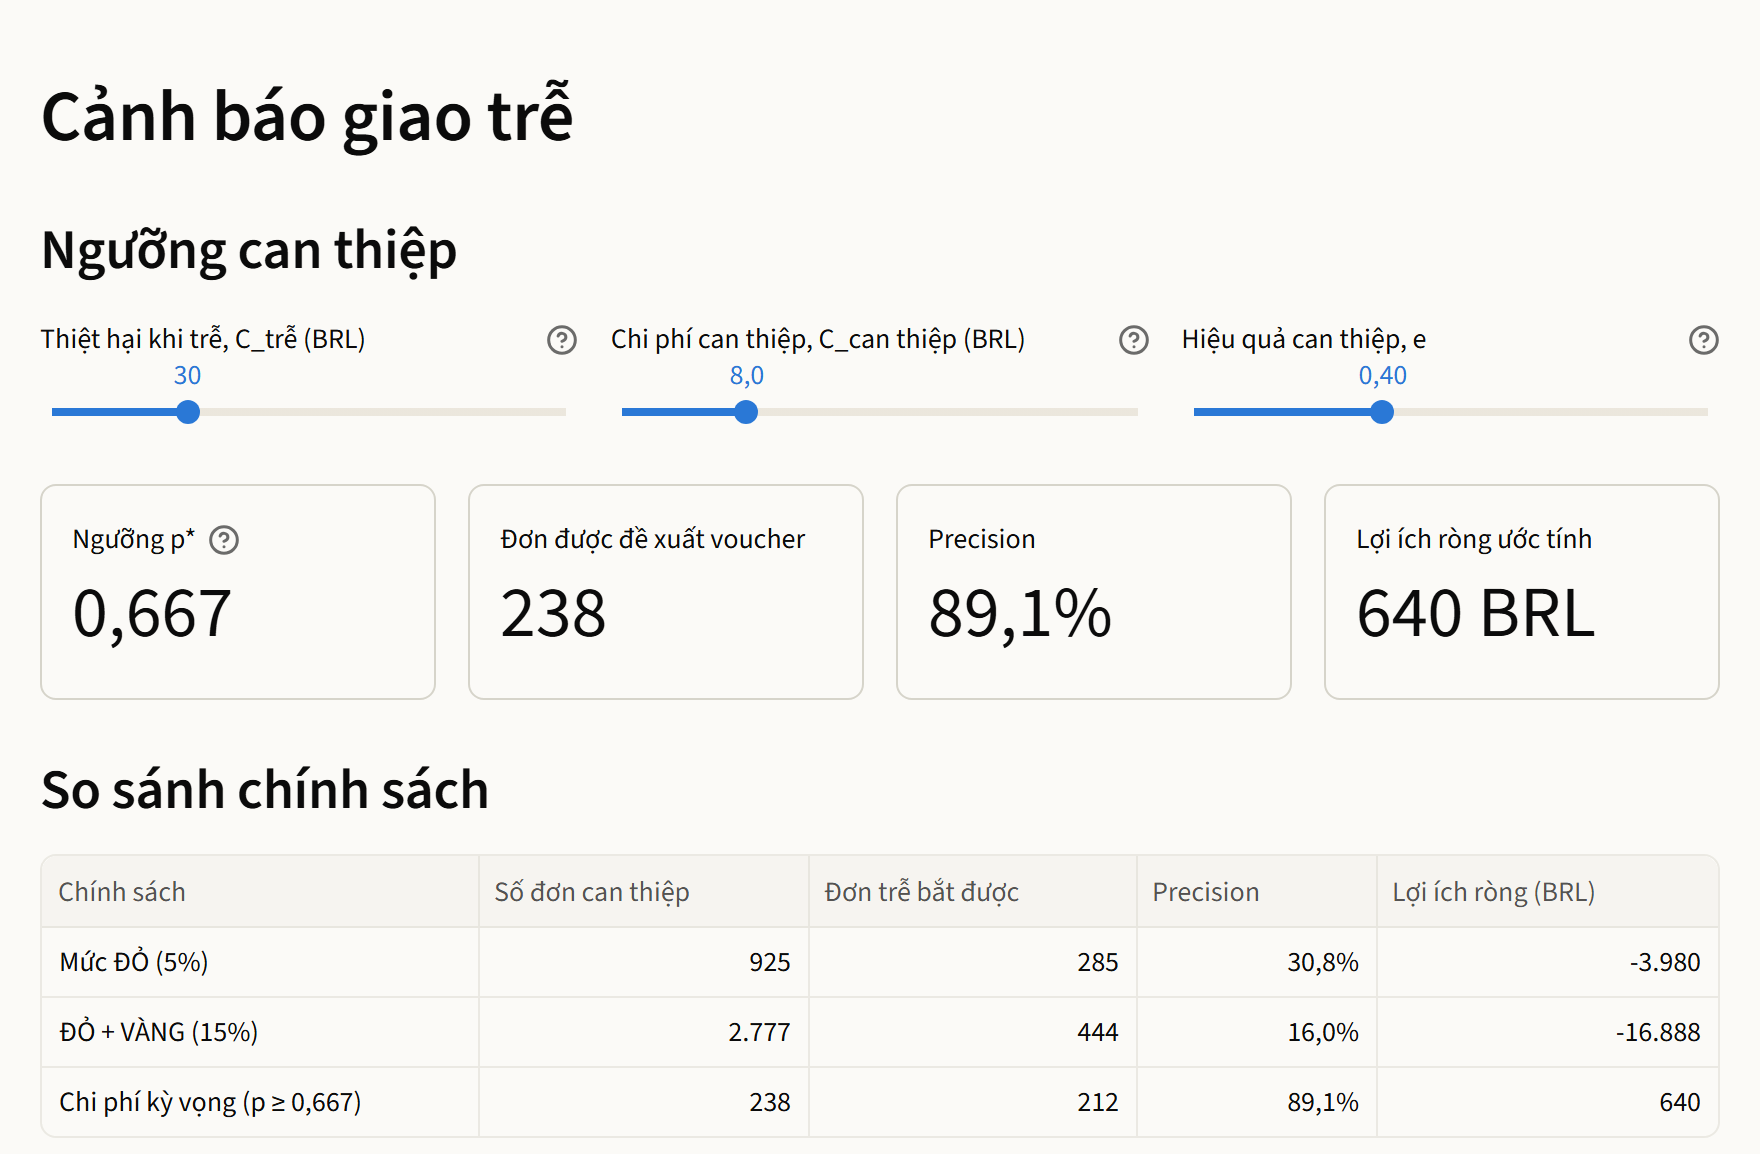
\includegraphics[width=\linewidth]{Pictures/dash-dss-whatif.png}
\caption{Trang Cảnh báo giao trễ, phần what-if: thanh trượt chi phí, ngưỡng $p^{*}$ và so sánh các chính sách}
\label{fig:dashdsswhatif}
\end{figure}

Phần dưới (Hình~\ref{fig:dashdssdanhsach}) là hàng đợi xử lý của một ngày bàn giao, lọc theo mức ĐỎ hoặc VÀNG. Mỗi đơn là một dòng gồm mức rủi ro, mã đơn, xác suất trễ, tối đa ba lý do kèm hành động đề xuất, trạng thái (chờ xử lý, đã duyệt hoặc đã từ chối) và nút thao tác; dòng đếm phía trên cho biết số đơn đã xử lý và còn chờ. Người vận hành nhập tên, có thể ghi chú, rồi bấm ``Duyệt'' hoặc ``Từ chối''; quyết định được ghi vào \code{dss.decision\_log} và đơn đó chuyển sang trạng thái đã duyệt kèm thời điểm, như đơn đầu tiên trên hình. Vì dữ liệu là ba tháng backtest, dòng ``Thực tế'' dưới mỗi đơn cho biết đơn đó sau cùng có trễ hay không; khi triển khai thật, thông tin này chưa có.

\begin{figure}[H]
\centering
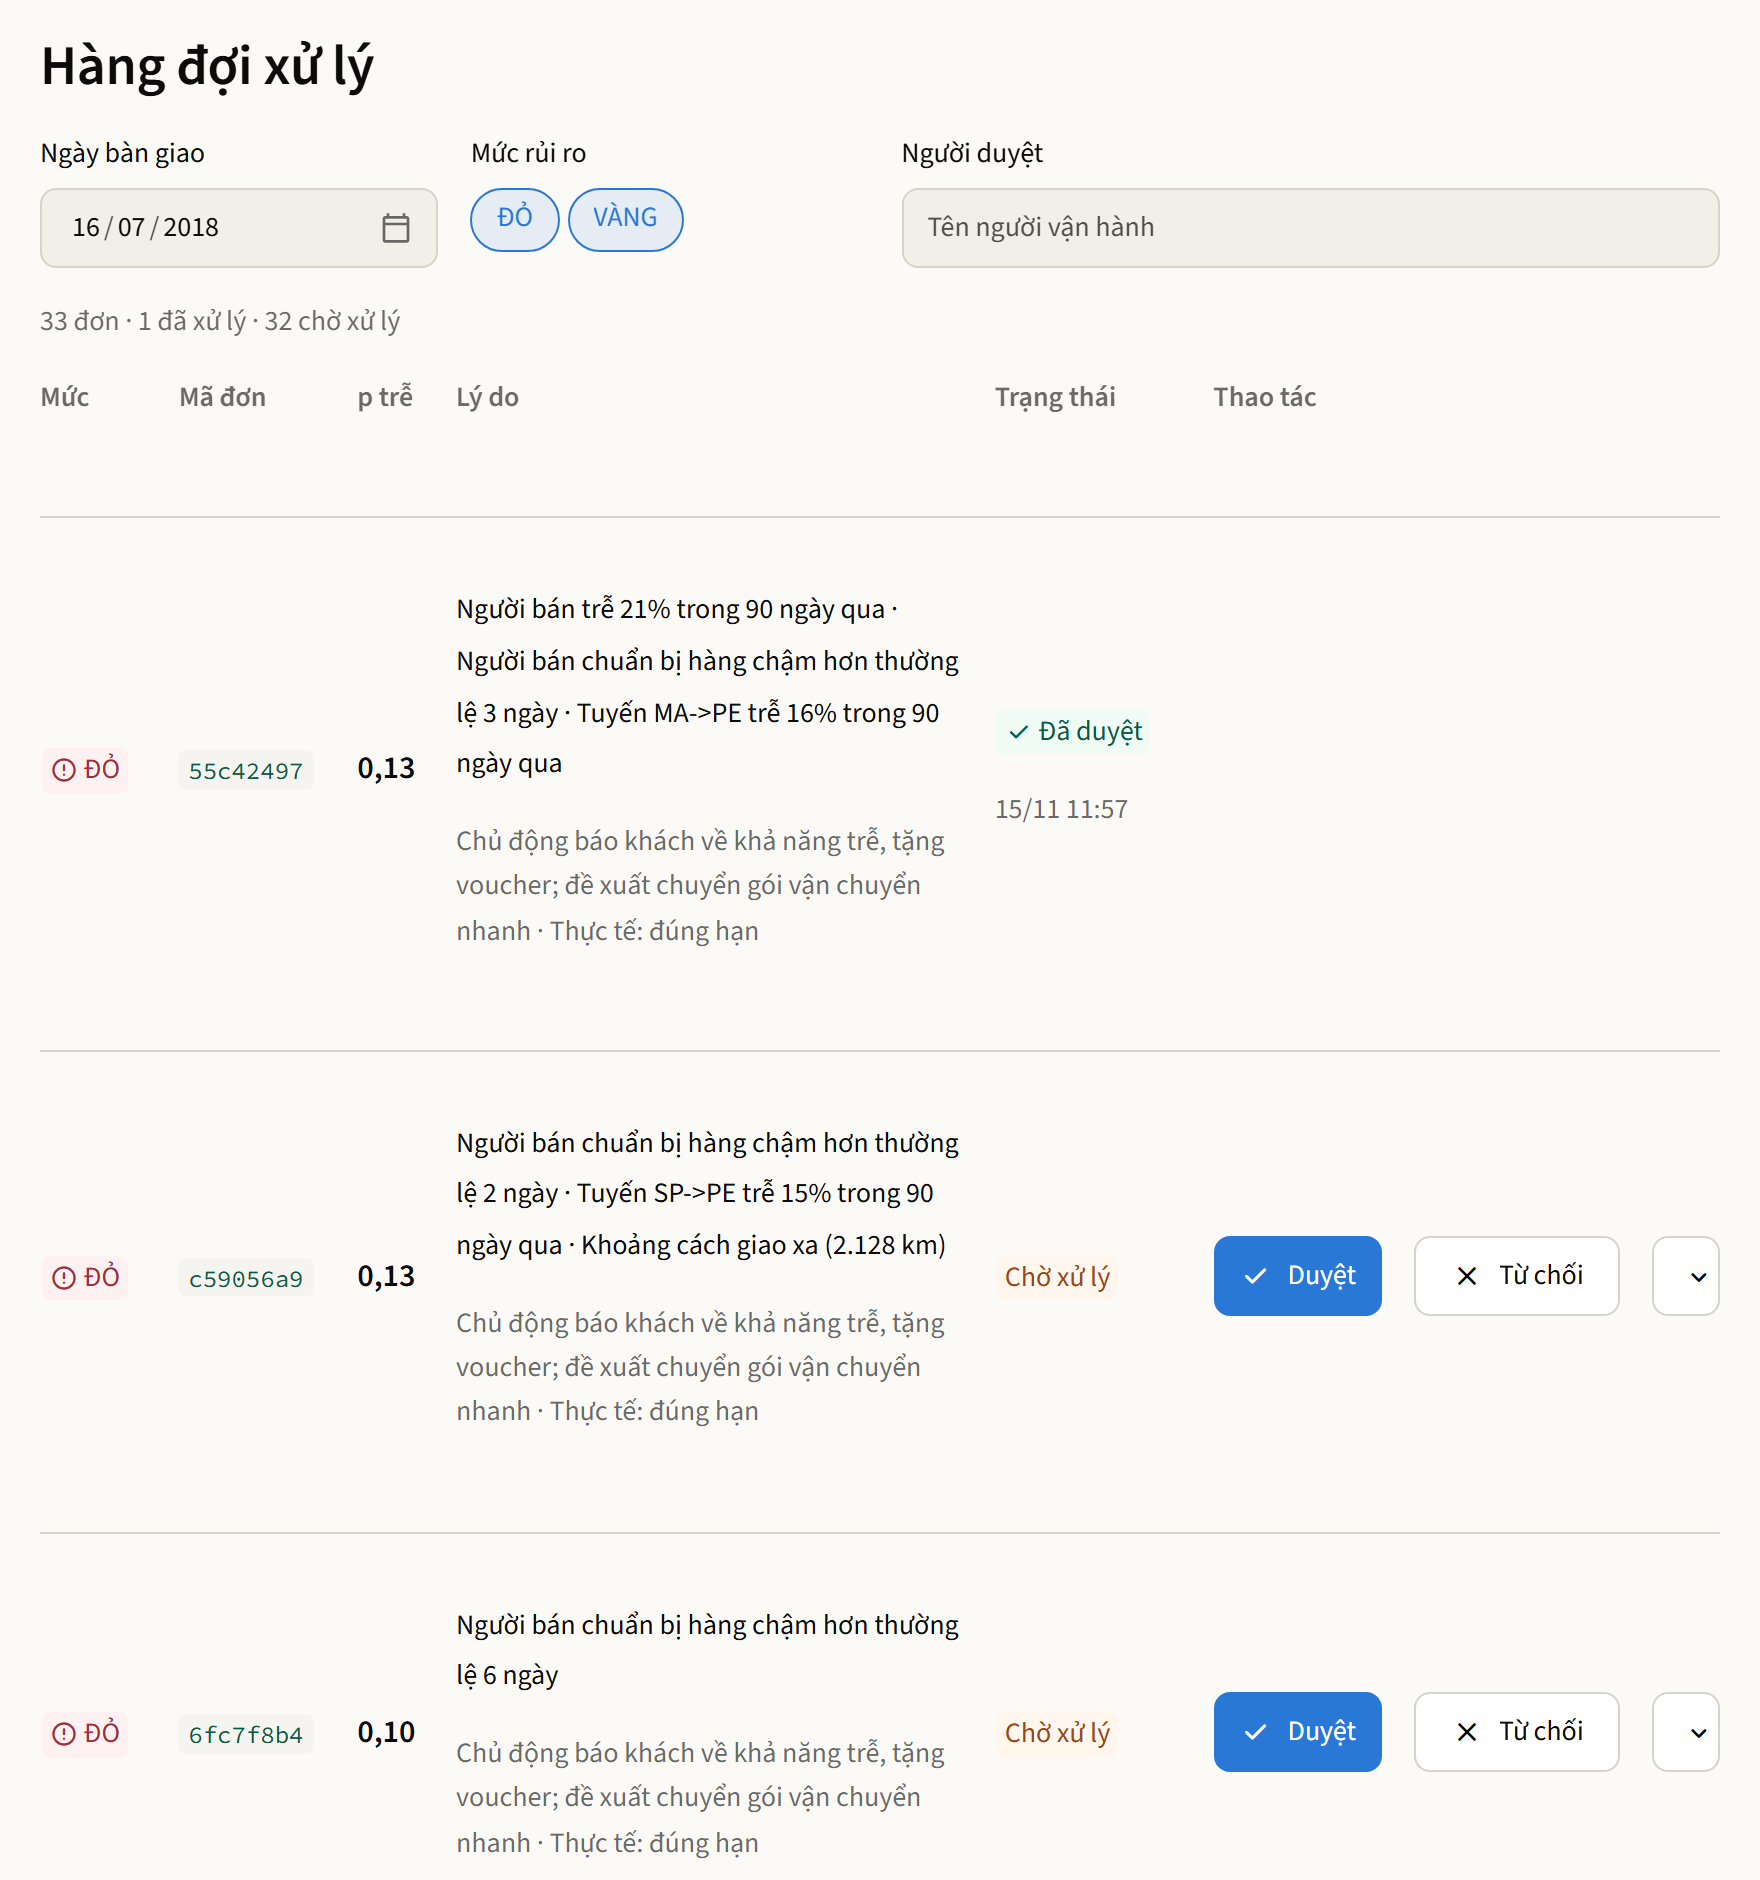
\includegraphics[width=\linewidth]{Pictures/dash-dss-danh-sach.png}
\caption{Trang Cảnh báo giao trễ, hàng đợi xử lý ngày 16/7/2018: lý do cảnh báo, hành động đề xuất, trạng thái và nút duyệt, từ chối}
\label{fig:dashdssdanhsach}
\end{figure}

\clearpage
% !TeX root = ../main.tex
\section{Đánh giá kết quả}\label{sec:danhgia}

\subsection{Kho dữ liệu}

Bảng~\ref{tab:danhgiakho} tổng hợp các phép kiểm tra đã chạy trên hệ thống thật ở phần hiện thực, cùng kết quả đo được.

\begingroup\small\setstretch{1.1}
\begin{longtable}{|P{3.0cm}|>{\raggedright\arraybackslash}p{5.2cm}|>{\raggedright\arraybackslash}p{5.5cm}|}
\caption{Kết quả kiểm tra kho dữ liệu}\label{tab:danhgiakho}\\
\hline
\textbf{Tiêu chí} & \textbf{Cách kiểm tra} & \textbf{Kết quả}\\ \hline \endfirsthead
\hline
\textbf{Tiêu chí} & \textbf{Cách kiểm tra} & \textbf{Kết quả}\\ \hline \endhead
Thời gian ETL & Nhật ký \code{meta.etl\_run\_log} của một lần nạp đầy đủ & 8,7 giây cho 1,55 triệu dòng nguồn (Bảng~\ref{tab:etlbuoc})\\ \hline
Khớp số liệu với nguồn & 20 tiêu chí đối soát trong \code{40\_dq\_checks.sql} & 20/20 tiêu chí đạt\\ \hline
Toàn vẹn tham chiếu & Ràng buộc khóa ngoại và bản ghi ``không xác định'' ($-1$) ở mọi bảng chiều & Mọi dòng của \code{fact\_sales} trỏ đến một bản ghi chiều hợp lệ\\ \hline
Truy vết bản ghi bị loại, bị sửa & Bảng \code{meta.rejected\_record} & 775 đơn bị loại và 1.458 bản ghi được sửa, mỗi bản ghi kèm lý do\\ \hline
Chạy lại nhiều lần & So số dòng và tổng tiền giữa các lần chạy & Không đổi, không trùng dữ liệu\\ \hline
Lỗi giữa chừng & \code{verify\_rollback.py} cố ý gây lỗi trước khi xác nhận giao dịch & Data Mart trở lại đủ 112.650 dòng\\ \hline
Tốc độ truy vấn OLAP & \code{EXPLAIN ANALYZE}, trung vị 5 lần chạy & Chậm nhất 0,72 giây (CUBE vùng và năm, Bảng~\ref{tab:thoigiantruyvan})\\ \hline
Phân quyền & Role \code{analyst\_ro}; thông tin kết nối trong \code{.env} & Người dùng phân tích chỉ có quyền \code{SELECT}\\ \hline
Metadata & Schema \code{meta} & Có từ điển dữ liệu và nguồn gốc của từng cột\\ \hline
Đúng số liệu trên dashboard & Đối chiếu tám chỉ số trên dashboard với kết quả OLAP và DSS & Cả tám chỉ số khớp (Bảng~\ref{tab:doichieu})\\ \hline
Thời gian phản hồi dashboard & Mở từng trang trong tiến trình mới bằng AppTest của Streamlit & Lần đầu 0,4-4,7 giây, lần sau dưới 0,1 giây\\ \hline
Tính khả dụng & Các thao tác lọc, drill-down, pivot, what-if trên dashboard & Người dùng chọn bằng thanh trượt, ô chọn và nút bấm, không cần viết SQL; tên chỉ số và chiều bằng tiếng Việt, số theo định dạng Việt Nam\\ \hline
Phân quyền dashboard & Thử \code{UPDATE}, \code{DELETE} bằng tài khoản \code{dashboard\_app} & Bị từ chối; dashboard chỉ được đọc và ghi thêm vào \code{dss.decision\_log}\\ \hline
\end{longtable}
\endgroup

Mọi nhu cầu theo dõi của bốn nhóm người dùng ở Bảng~\ref{tab:quyetdinh} đều có ít nhất một truy vấn OLAP trả lời: doanh thu theo thời gian, khu vực và ngành hàng (roll-up, slice, dice); tỷ lệ trễ theo bang và tuyến cùng thời gian từng công đoạn (drill-down, ma trận tuyến); điểm đánh giá theo ngành hàng, vùng và tình trạng giao hàng (pivot); người bán doanh thu cao nhưng chất lượng thấp và phân bố người bán so với khách hàng. Dashboard ở mục~\ref{sec:dashboard} đưa các chỉ số này lên giao diện để người dùng tự lọc và xem.

\subsection{Hệ hỗ trợ quyết định}

DSS đạt cả bốn chỉ tiêu đã đặt (Bảng~\ref{tab:datchitieu}): khi cảnh báo 10\% số đơn bàn giao mỗi ngày, mô hình bắt được 42,6\% số đơn sẽ trễ, và 46,5\% khi kết hợp với luật ``đã quá hạn''; kết quả ổn định qua cả ba tháng test, và đơn mức ĐỎ trễ nhiều gấp 13,0 lần đơn mức XANH. Mô hình được chọn sau khi so sánh năm ứng viên trên toàn bộ 14 tháng walk-forward, nơi nó có kết quả trung bình cao nhất (33,1\%); các ứng viên còn lại đạt 39,6-41,7\% trên test, cho thấy kết quả này không phụ thuộc vào một bộ tham số may mắn. Phân tích chi phí cho người quản lý một quy tắc dùng được ngay: hành động rẻ như báo trước cho khách nên làm cho mọi đơn ĐỎ, còn hành động đắt như tặng voucher chỉ nên dành cho các đơn vượt ngưỡng $p^{*}$. Với giả định chi phí mặc định, chính sách này có lợi ích ròng dương (640 BRL trên ba tháng test), trong khi tặng voucher cho cả 15\% đơn rủi ro nhất thì lỗ.

\clearpage
% !TeX root = ../main.tex
\section{Kết luận và hướng phát triển}\label{sec:ketluan}

\subsection{Kết luận}

Đề tài đã xây dựng một kho dữ liệu phân tích hiệu quả kinh doanh cho sàn thương mại điện tử Olist, đi từ phân tích nghiệp vụ đến một hệ thống chạy được trên toàn bộ 1,55 triệu dòng dữ liệu nguồn.

Phần khám phá dữ liệu tìm ra 31 vấn đề chất lượng cụ thể, từ dòng trùng trong dữ liệu địa lý đến mốc thời gian sai thứ tự, và cho thấy phần lớn giá trị thiếu có lý do nghiệp vụ; mỗi vấn đề có một quy tắc xử lý riêng, không làm mất bản ghi hợp lệ nào. Kho dữ liệu là một Data Mart xây theo hướng Bottom-up, snowflake schema với một bảng fact dạng accumulating snapshot ở mức dòng sản phẩm và bảy bảng chiều. Quy trình ETL chạy trọn trong 8,7 giây, đạt 20/20 tiêu chí đối soát, chạy lại không trùng dữ liệu và không để lại dữ liệu dở dang khi lỗi; 14 truy vấn OLAP bao phủ đủ năm phép toán và các nhu cầu theo dõi của người dùng, truy vấn chậm nhất mất 0,72 giây.

Phân tích OLAP chỉ ra giao trễ là nguyên nhân chính làm giảm mức độ hài lòng: tỷ lệ đánh giá 1-2 sao tăng từ 9,3\% lên 62,4\% khi đơn bị trễ, và giao trễ phụ thuộc rõ vào tuyến, mùa vụ và người bán. Dựa trên kết quả đó, thành phần hỗ trợ quyết định dự báo nguy cơ trễ của mỗi đơn ngay khi người bán bàn giao cho đơn vị vận chuyển, đề xuất đơn cần can thiệp theo năng lực xử lý hoặc theo chi phí kỳ vọng, và cho phép phân tích what-if với các giả định chi phí. DSS đạt cả bốn chỉ tiêu: khi cảnh báo 10\% số đơn, nó bắt được 42,6\% số đơn sẽ trễ (46,5\% khi kết hợp luật ``đã quá hạn''), ROC-AUC 0,744, và kết quả ổn định qua từng tháng test.

\subsection{Hạn chế và hướng phát triển}\label{sec:huongphattrien}

Bảng~\ref{tab:huongphattrien} liệt kê các hạn chế còn lại của hệ thống, mỗi hạn chế đi kèm hướng xử lý tương ứng.

\begingroup\small\setstretch{1.1}
\begin{longtable}{|P{1.9cm}|>{\raggedright\arraybackslash}p{5.9cm}|>{\raggedright\arraybackslash}p{5.9cm}|}
\caption{Hạn chế và hướng phát triển}\label{tab:huongphattrien}\\
\hline
\textbf{Phần} & \textbf{Hạn chế} & \textbf{Hướng phát triển}\\ \hline \endfirsthead
\hline
\textbf{Phần} & \textbf{Hạn chế} & \textbf{Hướng phát triển}\\ \hline \endhead
Dữ liệu & Không có giá vốn, chi phí vận hành và tên đơn vị vận chuyển, nên chưa tính được lợi nhuận và hành động ``chuyển gói vận chuyển nhanh'' chỉ là mô phỏng. & Bổ sung dữ liệu giá vốn và dữ liệu hành trình từ đơn vị vận chuyển khi có nguồn thật.\\ \hline
Dữ liệu & Giai đoạn ổn định chỉ khoảng 20 tháng; 42\% đơn đến từ bang SP nên số liệu ở các bang nhỏ dựa trên ít đơn; ở 1.278 đơn có nhiều người bán, mọi người bán dùng chung một mốc giao và một điểm đánh giá. & Thu thập thêm dữ liệu các năm sau để kiểm tra tính mùa vụ; hiển thị số đơn bên cạnh mọi tỷ lệ trên dashboard để người xem biết khi nào số liệu không đủ tin cậy.\\ \hline
Kho dữ liệu & Chưa có phần thanh toán. & Thêm Data Mart thanh toán dùng chung chiều thời gian và khách hàng, đưa kho về dạng fact constellation.\\ \hline
Kho dữ liệu & ETL nạp toàn bộ mỗi lần chạy, bảng chiều dùng SCD loại 1; hiệu năng mới đo ở quy mô hiện tại, và trang Giao hàng của dashboard đã mất 4,7 giây ở lần mở đầu. & Nạp tăng dần theo ngày mua, chuyển chiều khách hàng và người bán sang SCD loại 2, lập lịch bằng Airflow; thử với dữ liệu nhân bản nhiều lần và phân vùng bảng fact theo tháng nếu cần; tạo bảng tổng hợp lưu sẵn cho các truy vấn nặng nhất của dashboard (ma trận tuyến, thời gian từng công đoạn).\\ \hline
DSS & Mô hình yếu hơn ở các tháng trễ hàng loạt (24-27\% ở 11-12/2017 và 03/2018) và khi ít dữ liệu huấn luyện (15,6\% ở 07/2017). Năm ứng viên của đợt tìm kiếm mở rộng chỉ chênh nhau trong khoảng sai số (39,6-42,6\% trên test); việc chọn mô hình có dùng cả ba tháng test nên kết quả test có thể lạc quan hơn một chút. & Kết quả cho thấy giới hạn nằm ở dữ liệu chứ không ở thuật toán: cần dữ liệu hành trình và tình trạng của đơn vị vận chuyển; báo cáo chỉ tiêu kèm khoảng tin cậy bootstrap; khi có dữ liệu các tháng sau 08/2018, kiểm chứng lại mô hình đã chọn trên những tháng chưa tham gia vào việc chọn mô hình, gồm cả tháng bình thường lẫn tháng khủng hoảng.\\ \hline
DSS & Dự báo ngay lúc duyệt đơn mới bắt được khoảng 21-25\% đơn trễ ở mức cảnh báo 10\%, chưa đạt chỉ tiêu, vì phần lớn nguyên nhân gây trễ xảy ra sau thời điểm đó. & Khi có dữ liệu về năng lực kho của người bán, mở rộng sang cảnh báo sớm lúc duyệt đơn để nhắc người bán giao hàng sớm.\\ \hline
DSS & Chi phí can thiệp và hiệu quả của voucher là giả định; backtest chỉ giả lập trên dữ liệu lịch sử. & Thử nghiệm A/B khi triển khai để đo hiệu quả thật và cập nhật tham số chi phí.\\ \hline
DSS & 1.694 đơn chưa giao nhưng đã quá hạn được gán nhãn trễ theo giả định; lý do cảnh báo được sinh bằng luật từ các đặc trưng quan trọng. & Đối chiếu lại nhãn khi có trạng thái cuối của các đơn; dùng giải thích riêng cho từng đơn (như SHAP).\\ \hline
Mở rộng & Chưa dùng nội dung bình luận và chưa đánh giá người bán định kỳ. & Phân tích cảm xúc bình luận tiếng Bồ Đào Nha; chấm điểm người bán hằng tháng theo tỷ lệ trễ, tỷ lệ đánh giá thấp và thời gian chuẩn bị hàng.\\ \hline
\end{longtable}
\endgroup

\clearpage
% !TeX root = ../main.tex
\renewcommand{\refname}{Tài liệu tham khảo}
\addcontentsline{toc}{section}{Tài liệu tham khảo}
\begingroup
\sloppy
\begin{thebibliography}{9}
    \bibitem{inmon} W. H. Inmon, \textit{Building the Data Warehouse}, 4th ed. Wiley, 2005.
    \bibitem{kimball} R. Kimball, M. Ross, \textit{The Data Warehouse Toolkit}, 3rd ed. Wiley, 2013.
    \bibitem{turban} E. Turban, J. E. Aronson, T.-P. Liang, \textit{Decision Support Systems and Intelligent Systems}, 7th ed. Prentice-Hall, 2005.
    \bibitem{elmasri} R. Elmasri, S. B. Navathe, \textit{Fundamentals of Database Systems}, 7th ed. Addison-Wesley, 2016.
    \bibitem{sharda} R. Sharda, D. Delen, E. Turban, \textit{Analytics, Data Science, \& Artificial Intelligence: Systems for Decision Support}, 7th ed. Pearson, 2020.
    \bibitem{han} J. Han, M. Kamber, J. Pei, \textit{Data Mining: Concepts and Techniques}, 3rd ed. Morgan Kaufmann, 2012.
    \bibitem{burstein} F. Burstein, C. W. Holsapple, \textit{Handbook on Decision Support Systems}. Springer, 2008.
    \bibitem{tmq} Trần Minh Quang et al., \textit{Cơ sở dữ liệu: khái niệm, phương pháp, và kỹ thuật phân tích thiết kế}. NXB ĐHQG-HCM, 2025.
    \bibitem{olist} Olist, \textit{Brazilian E-Commerce Public Dataset by Olist}, Kaggle. Available: \url{https://www.kaggle.com/datasets/olistbr/brazilian-ecommerce}
\end{thebibliography}
\endgroup

\clearpage
\appendix
% !TeX root = ../main.tex
\section{Phụ lục: Hướng dẫn cài đặt và chạy hệ thống}\label{sec:phuluc}

Phụ lục này mô tả cách dựng lại toàn bộ hệ thống trên một máy mới, từ cơ sở dữ liệu đến các kết quả và biểu đồ trong báo cáo. Mã nguồn và dữ liệu nằm trong kho GitHub của nhóm tại \url{https://github.com/onhangocnhu/data-warehouse-assignment}; bộ dữ liệu gốc cũng có thể tải từ Kaggle.

\subsection{Yêu cầu phần mềm}

Máy cần có Docker (để chạy PostgreSQL 16), Python 3.11 trở lên (đã chạy thử với 3.14) và một bản phân phối \LaTeX{} có \code{pdflatex} với gói \code{vntex} nếu muốn biên dịch lại báo cáo và các biểu đồ. Các thư viện Python được liệt kê trong \code{src/requirements.txt}.

\subsection{Các bước chạy}

Tất cả lệnh dưới đây chạy từ thư mục gốc của kho mã nguồn. Bước 1 tạo tập tin cấu hình và khởi động cơ sở dữ liệu; nếu máy đã có sẵn một PostgreSQL chiếm cổng 5432, chỉ cần đổi \code{DB\_PORT} trong \code{.env} thành 5433.

\begin{lstlisting}[style=SQLStyle, language=bash]
# 1. Cấu hình và khởi động PostgreSQL 16 trong Docker
copy src\.env.example src\.env            # sửa DB_PASSWORD
docker compose -f src/docker-compose.yml up -d

# 2. Môi trường Python
python -m venv .venv
.venv\Scripts\activate            # Linux/macOS: source .venv/bin/activate
pip install -r src/requirements.txt

# 3. Tạo schema, bảng và chạy ETL đầy đủ (khoảng 10 giây)
python -m src.etl.run_etl --init
python -m src.etl.verify_rollback # (tùy chọn) kiểm tra tính toàn vẹn khi lỗi

# 4. EDA: khám phá dữ liệu thô và dữ liệu sau tiền xử lý
python -m src.eda.run_eda

# 5. OLAP: chạy 14 truy vấn, lưu kết quả và thời gian thực thi
python -m src.olap.run_olap

# 6. DSS: chọn mô hình, đánh giá walk-forward, chấm điểm đơn bàn giao
python -m src.dss.evaluate_models # thêm --reuse để dùng lại best_config.json
python -m src.dss.score_delay     # chạy sau bước trên

# 7. Sinh lại biểu đồ cho báo cáo (PNG 300 dpi)
python -m src.report.make_figures

# 8. Dashboard: tạo tài khoản dashboard_app (một lần) rồi mở http://localhost:8501
python -m src.dashboard.setup_role   # in 2 dòng DASHBOARD_DB_*, thêm vào .env
streamlit run src/dashboard/app.py
\end{lstlisting}

Bước 6 chạy lâu nhất (khoảng một giờ trên máy 20 luồng; \code{score\_delay} thêm khoảng 3 phút) vì phải thử 124 cấu hình trên năm tháng validation rồi huấn luyện lại mô hình cho từng tháng trong 14 tháng đánh giá; tham số được chọn được lưu ở \code{src/dss/results/best\_config.json}, nên lần chạy sau có thể bỏ qua bước tìm kiếm bằng tùy chọn \code{--reuse}. Toàn bộ chạy trên CPU, dùng dưới 2 GB bộ nhớ, không cần GPU. Có thể kiểm tra kết quả từng bước như sau: sau bước 3, \code{dm.fact\_sales} có 112.650 dòng và cả 20 tiêu chí trong \code{meta.dq\_result} đều đạt; sau bước 6, \code{dss.delay\_risk\_score} có 18.753 dòng.

Trên Linux hoặc macOS, có thể chạy dashboard bằng một lệnh \code{bash src/dashboard/run.sh}. Kịch bản này tự làm các bước 1, 2, 3, bước \code{score\_delay} (dùng \code{best\_config.json} có sẵn, không chạy lại bước tìm kiếm) và bước 8 nếu chúng chưa được làm, rồi mở dashboard; tùy chọn \code{--check} chỉ chuẩn bị và kiểm tra mà không mở dashboard.

Trên Windows bật Smart App Control, thư viện \code{psycopg} có thể bị chặn (lỗi \textit{DLL load failed\ldots Application Control policy}). Khi đó đặt biến môi trường \code{PSYCOPG\_IMPL=python} và thêm thư mục \code{bin} của một bản PostgreSQL cài trên máy vào \code{PATH} để dùng \code{libpq.dll} của bản đó.

\subsection{Cấu trúc mã nguồn}

\begin{lstlisting}[style=SQLStyle, language={}]
data/raw/                 9 tập tin CSV gốc của Olist
data/reference/           bảng vùng của 27 bang, bản dịch 2 ngành hàng còn thiếu
src/sql/                  00-05 tạo schema và bảng; 10 transform; 20 nạp bảng chiều;
                          30 nạp bảng fact; 40 kiểm tra chất lượng; 50 truy vấn OLAP
src/etl/                  run_etl.py (điều phối), extract.py (COPY), db.py (nhật ký),
                          verify_rollback.py
src/eda/                  run_eda.py; results/ chứa kết quả khám phá dữ liệu
src/olap/                 run_olap.py; results/ chứa kết quả và thời gian từng truy vấn
src/dss/                  features.py (đặc trưng point-in-time), evaluate_models.py,
                          score_delay.py; results/ chứa kết quả đánh giá
src/dashboard/            app.py (điều hướng), db.py, filters.py, ui.py, views/ (7 trang),
                          setup_role.py, run.sh (chạy dashboard bằng một lệnh)
src/report/               make_figures.py: sinh biểu đồ của báo cáo từ cơ sở dữ liệu
report/                   mã nguồn LaTeX của báo cáo; Sections/hinh/ chứa các sơ đồ TikZ
src/docker-compose.yml    PostgreSQL 16
\end{lstlisting}

\section{Phụ lục: Bảng mã bang của Brazil}\label{sec:mabang}

Bảng~\ref{tab:mabang} liệt kê 27 đơn vị hành chính cấp bang của Brazil (26 bang và Quận Liên bang DF) theo mã hai chữ cái dùng trong dữ liệu và trong báo cáo, cùng vùng mà nhóm gán cho từng bang trong bảng chiều \code{dim\_state}.

\begin{table}[H]
\centering
\small
\caption{Mã, tên và vùng của 27 bang Brazil}\label{tab:mabang}
\begin{tabular}{|c|l|l||c|l|l|}
\hline
\textbf{Mã} & \textbf{Tên bang} & \textbf{Vùng} & \textbf{Mã} & \textbf{Tên bang} & \textbf{Vùng}\\ \hline
AC & Acre & Norte & PB & Paraíba & Nordeste\\ \hline
AL & Alagoas & Nordeste & PE & Pernambuco & Nordeste\\ \hline
AM & Amazonas & Norte & PI & Piauí & Nordeste\\ \hline
AP & Amapá & Norte & PR & Paraná & Sul\\ \hline
BA & Bahia & Nordeste & RJ & Rio de Janeiro & Sudeste\\ \hline
CE & Ceará & Nordeste & RN & Rio Grande do Norte & Nordeste\\ \hline
DF & Distrito Federal & Centro-Oeste & RO & Rondônia & Norte\\ \hline
ES & Espírito Santo & Sudeste & RR & Roraima & Norte\\ \hline
GO & Goiás & Centro-Oeste & RS & Rio Grande do Sul & Sul\\ \hline
MA & Maranhão & Nordeste & SC & Santa Catarina & Sul\\ \hline
MG & Minas Gerais & Sudeste & SE & Sergipe & Nordeste\\ \hline
MS & Mato Grosso do Sul & Centro-Oeste & SP & São Paulo & Sudeste\\ \hline
MT & Mato Grosso & Centro-Oeste & TO & Tocantins & Norte\\ \hline
PA & Pará & Norte & & & \\ \hline
\end{tabular}
\end{table}


\end{document}
